% =====================================================================
%  Објектно оријентисано програмирање — Програмски језик Јава, том 2
%  LaTeX извор (memoir + listings + XeLaTeX)
% =====================================================================
\documentclass[11pt,a4paper,openright,twoside]{memoir}

% --- Кодирање и језик ---------------------------------------------------
\usepackage{fontspec}
\usepackage{polyglossia}
\setdefaultlanguage{serbian}
\setotherlanguage{english}

% Главни фонт — PT Serif (топао serif, пуна ћирилица).
\setmainfont{DejaVu Serif}[
  Ligatures=TeX,
  Scale=0.95
]
\setsansfont{DejaVu Sans}[Scale=0.92]
\setmonofont{DejaVu Sans Mono}[Scale=0.85]

% Размак између линија (као у memoir 6x9 темплејту)
\linespread{1.22}
\frenchspacing

% --- Изглед странице (memoir) -------------------------------------------
\setstocksize{297mm}{210mm}
\settrimmedsize{297mm}{210mm}{*}
\settrims{0pt}{0pt}
\setlrmarginsandblock{28mm}{22mm}{*}
\setulmarginsandblock{25mm}{30mm}{*}
\setheadfoot{14pt}{36pt}
\setheaderspaces{*}{12pt}{*}
\checkandfixthelayout

% --- Стилови поглавља (као у стандардном LaTeX book class-у) ------------
\makechapterstyle{bookmatch}{%
  \renewcommand{\chapnumfont}{\normalfont\huge\bfseries\raggedright}
  \renewcommand{\chaptitlefont}{\normalfont\Huge\bfseries\raggedright}
  \renewcommand{\printchaptername}{\chapnumfont\chaptername}
  \renewcommand{\chapternamenum}{\space}
  \renewcommand{\printchapternum}{\chapnumfont\thechapter}
  \renewcommand{\afterchapternum}{\par\nobreak\vskip 20pt}
  \renewcommand{\printchaptertitle}[1]{\chaptitlefont ##1}
  \renewcommand{\afterchaptertitle}{%
    \par\nobreak\vskip 12pt%
    {\color{black!50}\hrule height 0.4pt}%
    \par\nobreak\vskip 30pt}
}
\chapterstyle{bookmatch}
\setsecnumdepth{subsection}
\settocdepth{section}
\renewcommand{\chaptername}{Поглавље}

% Шира поља за бројеве у садржају (да 11.10, 19.12 не прелазе у текст)
\setlength{\cftchapternumwidth}{2.4em}
\setlength{\cftsectionnumwidth}{3.4em}
\setlength{\cftsubsectionnumwidth}{4.2em}
\renewcommand{\cftchapterfont}{\normalfont\bfseries}
\renewcommand{\cftsectionfont}{\normalfont}

% Прелом речи и микротиповe
\usepackage{microtype}
\emergencystretch=3em
\tolerance=1500
\hbadness=10000
\hyphenpenalty=50
\exhyphenpenalty=50
\sloppybottom

% --- Заглавље/подножје --------------------------------------------------
\makepagestyle{oopstyle}
% Парне стране: број странице лево, име поглавља (мала капитала) десно
\makeevenhead{oopstyle}{\small\thepage}{}{\small\scshape\leftmark}
% Непарне стране: исти наслов поглавља лево, број странице десно
\makeoddhead{oopstyle}{\small\scshape\leftmark}{}{\small\thepage}
\makeheadrule{oopstyle}{\textwidth}{0.4pt}
\makeevenfoot{oopstyle}{}{}{}
\makeoddfoot{oopstyle}{}{}{}
\pagestyle{oopstyle}

% --- Боје и листинзи ----------------------------------------------------
\usepackage{xcolor}
\definecolor{codebg}{HTML}{F5F5F5}
\definecolor{codeframe}{HTML}{CCCCCC}
\definecolor{codekw}{HTML}{0033B3}
\definecolor{codestr}{HTML}{067D17}
\definecolor{codecomment}{HTML}{8C8C8C}
\definecolor{codetype}{HTML}{000080}

\usepackage{listings}
% XeLaTeX + fontspec обрађују UTF-8 нативно, тако да `literate` мапирања
% за ћирилицу нису потребна. Важно је само да `extendedchars=true` и
% `inputencoding=utf8` буду постављени.
\lstset{
  language=Java,
  basicstyle=\ttfamily\small,
  keywordstyle=\color{codekw}\bfseries,
  stringstyle=\color{codestr},
  commentstyle=\color{codecomment},
  numbers=none,
  showstringspaces=false,
  tabsize=4,
  breaklines=true,
  breakatwhitespace=false,
  backgroundcolor=\color{codebg},
  frame=single,
  rulecolor=\color{codeframe},
  framesep=4pt,
  xleftmargin=14pt,
  xrightmargin=4pt,
  aboveskip=14pt,
  belowskip=14pt,
  extendedchars=true,
  inputencoding=utf8,
  upquote=true,
  columns=fullflexible,
  keepspaces=true,
}

% --- Хипервезе ----------------------------------------------------------
\usepackage[hidelinks,unicode]{hyperref}
\hypersetup{
  pdftitle={Објектно оријентисано програмирање — Јава, том 2},
  pdfauthor={Сташа Вујичић Станковић и сарадници},
  pdfsubject={Уџбеник из ООП-а},
  pdflang={sr},
  bookmarksopen=true
}

% --- Графика и тaбеле ---------------------------------------------------
\usepackage{amssymb}
\usepackage{needspace}
\usepackage{graphicx}
\usepackage{float}  % za [H] placement
\usepackage{enumitem}
\graphicspath{{./figures/}}
\usepackage{longtable}
\usepackage{booktabs}
\usepackage{array}

% --- Прилагођене команде ------------------------------------------------
\newcommand{\primer}[1]{\noindent\textbf{Пример #1.}\enspace}

% =====================================================================
\begin{document}

\frontmatter
\begin{titlingpage}
  \begin{center}
    {\Large Универзитет у Београду}\\
    {\large Математички факултет}\\[3cm]
    {\Huge\bfseries ОБЈЕКТНО ОРИЈЕНТИСАНО ПРОГРАМИРАЊЕ}\\[0.8cm]
    {\LARGE ПРОГРАМСКИ ЈЕЗИК ЈАВА -- 2}\\[\fill]\vspace*{2cm}
    {\Large Сташа Вујичић Станковић}\\[0.15cm]
    {\Large Владимир Филиповић}\\[0.15cm]
    {\Large Александар Картељ}\\[0.15cm]
    {\Large Душан Тошић}\\[\fill]
    {\large Београд, 2026.}
  \end{center}
\end{titlingpage}

\tableofcontents
\clearpage

\mainmatter





\chapter*{Предговор}
\addcontentsline{toc}{chapter}{Предговор}
\markboth{Предговор}{Предговор}
\thispagestyle{plain}


Кроз задатке се спирално развијају исте теме, само што постају сложенији...


Укључују се ламбда-изрази и др. карактеристике које постоје код Јава 8

За ГУИ се описује само Јava FX

Развојно окружење са којим се ради је IntelliJ Idea


Називи пакета у примерима и задацима треба да одговарају ознакама поглавља


Укључити све што је морало да се изв+баци из тома 1 (и то на почетку)  -  догађаје, анотације и процесирање анотација, вишенитно програмирање, серијализацију, функционално програмирање

интеграција са базама података, ОR мапирање, сервлети и веб сервиси?


Размотрити да ли негде да се убаци и рад са регулерним изразима у Јави

[1] [2] 


                          Аутори[3] [4] 




\setlength{\parindent}{15pt}
\setlength{\parskip}{0pt}
\chapter{Рефлексија (самоиспитивање)}

Библиотека за \textbf{рефлексију} (енг. \textit{reflection}) пружа веома богат и разрађен скуп алата за писање програма који динамички манипулишу Јава кодом. Ова могућност се интензивно користи код \textit{JavaBeans} компоненти (в. поглавље 8), оквира за тестирање, ORM библиотека, механизама за серијализацију и сличних алата. Коришћењем рефлексије, Јава може да подржи алате сличне онима које корисници Visual Basic-а одавно имају. Нарочито, када се нове класе додају у време пројектовања или извршавања, алати за развој апликација могу динамички да испитују могућности тих класа.

Програм који може да анализира могућности класа назива се \textit{рефлективни} (енг. \textit{reflective}). Механизам рефлексије је изузетно моћан и може се користити за: анализу могућности класа у време извршавања, испитивање објеката у време извршавања (нпр. писање универзалног toString() метода), имплементацију генеричке манипулације низовима, динамичко креирање објеката и позивање метода, као и испитивање и обраду забелешки (анотација).

Рефлексија је моћан и комплексан механизам. Међутим, она је превасходно од интереса за програмере развојних алата, а не за апликационе програмере. У овом поглављу биће детаљно обрађене класе и методи из пакета \texttt{java.lang.reflect}, уз бројне примере који илуструју практичну примену рефлексије.

\section{Класе за рефлексију}

Централна класа у механизму рефлексије је \texttt{java.lang.Class}. Док програм ради, Јава извршно окружење одржава тзв. \textbf{идентификацију типа у време извршавања} (енг. \textit{Runtime Type Identification, RTTI}) за све објекте. Ова информација чува податак о класи којој сваки објекат припада. Виртуелна машина користи информацију о типу да одабере одговарајуће методе за извршавање.

Класа \texttt{Class} описује својства одређене класе. Објекат типа \texttt{Class} се може добити на три начина.

Први начин је позивом метода \texttt{getClass()} над било којим објектом.  Овај метод је дефинисан у класи \texttt{Object} и наслеђују га све класе:

\needspace{5\baselineskip}
\begin{lstlisting}[language=Java]
String s = "Здраво";
Class<?> c1 = s.getClass();
System.out.println(c1.getName()); // java.lang.String
\end{lstlisting}


Други начин је коришћењем литерала \texttt{.class} над именом типа:

\needspace{5\baselineskip}
\begin{lstlisting}[language=Java]
Class<?> c2 = String.class;
Class<?> c3 = int.class;
Class<?> c4 = Double[].class;
\end{lstlisting}


Трећи начин је позивом статичког метода \texttt{Class.forName()} са потпуним именом класе као аргументом:

\needspace{5\baselineskip}
\begin{lstlisting}[language=Java]
Class<?> c5 = Class.forName("java.util.Date");
\end{lstlisting}


Метод \texttt{forName()} избацује \texttt{ClassNotFoundException} ако класа са задатим именом не постоји, па је потребно обрадити овај изузетак. Овај начин је посебно користан када је име класе сачувано у ниски чија вредност може варирати у време извршавања.

Виртуелна машина управља јединственим \texttt{Class} објектом за сваки тип. Стога се за поређење објеката типа \texttt{Class} може користити оператор \texttt{==}:

\needspace{5\baselineskip}
\begin{lstlisting}[language=Java]
if (e.getClass() == Employee.class) { ... }
\end{lstlisting}


Нeки од најважнијих метода класе \texttt{Class} су:

\texttt{String getName()} – враћа име класе (укључујући име пакета)

\texttt{Class\textless{}?\textgreater{} getSuperclass()} – враћа наткласу

\texttt{Class\textless{}?\textgreater{}[] getInterfaces()} – враћа низ интерфејса које класа имплементира

\texttt{boolean isArray()} – проверава да ли тип представља низ

\texttt{boolean isInterface()} – проверава да ли је тип интерфејс

\texttt{boolean isPrimitive()} – проверава да ли је тип примитиван

\texttt{Class\textless{}?\textgreater{} getComponentType()} – враћа тип елемента низа

\texttt{int getModifiers()} – враћа модификаторе класе (public, abstract, final, итд.)


\bigskip

\noindent \textbf{Пример 1.} Испитивање типа у време извршавања. $\square$

\medskip

Следећи програм демонстрира основне могућности класе \texttt{Class} – добијање објекта \texttt{Class} на три начина, испитивање наткласе, интерфејса, као и провера типа:

\needspace{5\baselineskip}
\begin{lstlisting}[language=Java]
package rs.math.oop.g01.p01.ispitivanjeTipa;
import java.lang.reflect.*;
 
public class Primer01_IspitivanjeTipa {
   public static void main(String[] args) {
         // Добијање објекта класе Class на три начина
 
         // 1. Преко метода getClass()
         String s = "Здраво";
         Class<?> c1 = s.getClass();
         System.out.println("1. Преко getClass(): " + c1.getName());
 
         // 2. Преко литерала .class
         Class<?> c2 = String.class;
         System.out.println("2. Преко .class: " + c2.getName());
 
         // 3. Преко статичког метода Class.forName()
         try {
          Class<?> c3 = Class.forName("java.util.Date");
          System.out.println("3. Преко forName(): " + c3.getName());
         } catch (ClassNotFoundException e) {
          e.printStackTrace();
         }
 
         // Испитивање наткласе
         System.out.println("\nНаткласа од Integer: "
                + Integer.class.getSuperclass().getName());
 
         // Провера типа помоћу instanceof и getClass()
         Number n = Integer.valueOf(42);
         System.out.println("\nn instanceof Number: " + (n instanceof Number));
         System.out.println("n.getClass() == Integer.class: "
                + (n.getClass() == Integer.class));
 
         // Испитивање интерфејса
         Class<?>[] interfejsi = Integer.class.getInterfaces();
         System.out.println("\nИнтерфејси класе Integer:");
         for (Class<?> i : interfejsi) {
          System.out.println("  " + i.getName());
         }
 
         // Испитивање низова
         int[] niz = {1, 2, 3};
         System.out.println("\nТип низа int[]: " + niz.getClass().getName());
         System.out.println("Да ли је низ: " + niz.getClass().isArray());
         System.out.println("Тип елемента низа: "
                + niz.getClass().getComponentType().getName());
   }
}
\end{lstlisting}


Извршавањем овог програма добија се следећи резултат:

\needspace{5\baselineskip}
\begin{lstlisting}[language=Java]
1. Преко getClass(): java.lang.String
2. Преко .class: java.lang.String
3. Преко forName(): java.util.Date
 
Наткласа од Integer: java.lang.Number
 
n instanceof Number: true
n.getClass() == Integer.class: true
 
Интерфејси класе Integer:
  java.lang.Comparable
  java.lang.constant.Constable
  java.lang.constant.ConstantDesc
 
Тип низа int[]: [I
Да ли је низ: true
Тип елемента низа: int
\end{lstlisting}

\subsection{Рефлексија и низови}

Класа \texttt{java.lang.reflect.Array} пружа статичке методе за динамичко креирање и манипулацију низовима. Главни методи су:

\texttt{Array.newInstance(Class\textless{}?\textgreater{} componentType, int length)} – креира нови низ задатог типа и дужине. \texttt{Array.getLength(Object array)} – враћа дужину низа. Методи \texttt{Array.get()}, \texttt{Array.set()}, \texttt{Array.getInt()}, \texttt{Array.setInt()} и слични омогућавају читање и постављање елемената.

Ова могућност је посебно корисна за писање генеричких метода који раде са низовима произвољног типа. На пример, метод за проширивање низа мора да креира нови низ истог типа као оригинални – што без рефлексије није могуће на генерички начин.


\bigskip

\noindent \textbf{Пример 2.} Рефлексија и низови. $\square$

\medskip

Следећи програм демонстрира динамичко креирање низова и генерички метод за проширивање низа:

\needspace{5\baselineskip}
\begin{lstlisting}[language=Java]
package rs.math.oop.g01.p02.refleksijaNizovi;
import java.lang.reflect.Array;
 
public class Primer02_RefleksijaNizovi {
   public static void main(String[] args) {
         // Динамичко креирање низа
         Object niz = Array.newInstance(int.class, 5);
         for (int i = 0; i < 5; i++) {
          Array.setInt(niz, i, (i + 1) * 10);
         }
         System.out.println("Динамички креиран низ int[]:");
         for (int i = 0; i < Array.getLength(niz); i++) {
          System.out.print("  " + Array.getInt(niz, i));
         }
         System.out.println();
 
         // Генерички метод за проширивање низа
         int[] original = {1, 2, 3, 4, 5};
         int[] prosiren = (int[]) prosiriNiz(original, 10);
         System.out.println("\nПроширени низ (дужина "
                + prosiren.length + "):");
         for (int v : prosiren) {
          System.out.print("  " + v);
         }
         System.out.println();
   }
 
   public static Object prosiriNiz(Object niz, int novaDuzina) {
         Class<?> tipKlase = niz.getClass();
         if (!tipKlase.isArray())
          throw new IllegalArgumentException("Није низ!");
         Class<?> tipElementa = tipKlase.getComponentType();
         int staraDuzina = Array.getLength(niz);
         Object noviNiz = Array.newInstance(tipElementa, novaDuzina);
         System.arraycopy(niz, 0, noviNiz, 0,
                Math.min(staraDuzina, novaDuzina));
         return noviNiz;
   }
}
\end{lstlisting}


Извршавањем овог програма добија се:

\needspace{5\baselineskip}
\begin{lstlisting}[language=Java]
Динамички креиран низ int[]:
  10  20  30  40  50
 
Проширени низ (дужина 10):
  1  2  3  4  5  0  0  0  0  0
\end{lstlisting}

\subsection{Рефлексија и генерици}

Иако Јава користи \textbf{брисање типова} (енг. \textit{type erasure}) при компилацији генеричког кода, информације о генеричким типовима су и даље сачуване у метаподацима класе и доступне су преко рефлексије. Пакет \texttt{java.lang.reflect} садржи интерфејсе за представљање генеричких типова:

\texttt{Type} – надинтерфејс за све типове

\texttt{ParameterizedType} – параметризовани тип (нпр. \texttt{List\textless{}String\textgreater{}})

\texttt{TypeVariable} – типска променљива (нпр. \texttt{T extends Number})

\texttt{WildcardType} – џокер тип (нпр. \texttt{? extends Number})

\texttt{GenericArrayType} – генерички тип низа


\bigskip

\noindent \textbf{Пример 3.} Рефлексија и генерици. $\square$

\medskip

Следећи програм испитује генеричке типове поља и метода:

\needspace{5\baselineskip}
\begin{lstlisting}[language=Java]
package rs.math.oop.g01.p03.refleksijaGenerici;
import java.lang.reflect.*;
import java.util.List;
import java.util.Map;
 
class Skladiste {
   private List<String> imena;
   private Map<String, Integer> ocene;
   public List<String> getImena() { return imena; }
   public void obradiMapu(Map<String, List<Integer>> mapa) {}
}
 
public class Primer03_RefleksijaGenerici {
   public static void main(String[] args) throws Exception {
         Class<?> klasa = Skladiste.class;
 
         for (Field f : klasa.getDeclaredFields()) {
          Type gt = f.getGenericType();
          System.out.println("Поље: " + f.getName());
          System.out.println("  Генерички тип: " + gt);
          if (gt instanceof ParameterizedType) {
                ParameterizedType pt = (ParameterizedType) gt;
                Type[] args2 = pt.getActualTypeArguments();
                System.out.print("  Аргументи типа: ");
                for (int i = 0; i < args2.length; i++) {
                if (i > 0) System.out.print(", ");
                System.out.print(args2[i].getTypeName());
                }
                System.out.println();
          }
         }
   }
}
\end{lstlisting}


Извршавањем програма добија се:

\needspace{5\baselineskip}
\begin{lstlisting}[language=Java]
Поље: imena
  Генерички тип: java.util.List<java.lang.String>
  Аргументи типа: java.lang.String
Поље: ocene
  Генерички тип: java.util.Map<java.lang.String, java.lang.Integer>
  Аргументи типа: java.lang.String, java.lang.Integer
\end{lstlisting}

\section{Испитивање типа у време извршавања}

Три класе из пакета \texttt{java.lang.reflect}, \texttt{Field}, \texttt{Method} и \texttt{Constructor}, описују поља, методе и конструкторе класе. Свака од ових класа има метод \texttt{getName()} који враћа име одговарајућег елемента. Класа \texttt{Field} има метод \texttt{getType()} који враћа тип поља. Класе \texttt{Method} и \texttt{Constructor} имају методе за добијање типова параметара и повратног типа. Све три класе имају метод \texttt{getModifiers()} који враћа целобројну вредност чији битови описују модификаторе (\texttt{public}, \texttt{private}, \texttt{static} итд.). За анализу модификатора користи се класа \texttt{Modifier}.

\subsection{Испитивање поља објекта}

Класа \texttt{Class} пружа два метода за добијање информација о пољима: \texttt{getFields()} враћа низ јавних поља (укључујући наслеђена), док \texttt{getDeclaredFields()} враћа сва поља декларисана у датој класи (укључујући приватна и заштићена), али без наслеђених.


\bigskip

\noindent \textbf{Пример 4.} Испитивање поља објекта помоћу рефлексије. $\square$

\medskip

\needspace{5\baselineskip}
\begin{lstlisting}[language=Java]
package rs.math.oop.g01.p04.ispitivanjePolja;
import java.lang.reflect.Field;
import java.lang.reflect.Modifier;
 
class Zaposleni {
   private String ime;
   private double plata;
   protected int godineStaza;
   public String odeljenje;
 
   public Zaposleni(String ime, double plata,
          int godineStaza, String odeljenje) {
         this.ime = ime;
         this.plata = plata;
         this.godineStaza = godineStaza;
         this.odeljenje = odeljenje;
   }
}
 
class Menadzer extends Zaposleni {
   private double bonus;
 
   public Menadzer(String ime, double plata,
          int godineStaza, String odeljenje, double bonus) {
         super(ime, plata, godineStaza, odeljenje);
         this.bonus = bonus;
   }
}
 
public class Primer04_IspitivanjePolja {
   public static void main(String[] args) {
         Class<?> klasa = Menadzer.class;
 
         System.out.println("=== Поља класе "
                + klasa.getSimpleName() + " ===");
         Field[] deklarisana = klasa.getDeclaredFields();
         for (Field f : deklarisana) {
          System.out.println("  "
                + Modifier.toString(f.getModifiers())
                + " " + f.getType().getSimpleName()
                + " " + f.getName());
         }
 
         System.out.println("\n=== Поља наткласе ===");
         for (Field f : klasa.getSuperclass()
                .getDeclaredFields()) {
          System.out.println("  "
                + Modifier.toString(f.getModifiers())
                + " " + f.getType().getSimpleName()
                + " " + f.getName());
         }
   }
}
\end{lstlisting}


Извршавањем програма добија се:

\needspace{5\baselineskip}
\begin{lstlisting}[language=Java]
=== Поља класе Menadzer ===
  private double bonus
 
=== Поља наткласе ===
  private String ime
  private double plata
  protected int godineStaza
  public String odeljenje
\end{lstlisting}

\subsection{Испитивање метода објекта}

Аналогно пољима, класа \texttt{Class} пружа методе \texttt{getMethods()} и \texttt{getDeclaredMethods()} за добијање информација о методима. За сваки метод може се испитати: име, повратни тип, типови параметара, модификатори, као и да ли метод избацује изузетке.


\bigskip

\noindent \textbf{Пример 5.} Испитивање метода класе. $\square$

\medskip

\needspace{5\baselineskip}
\begin{lstlisting}[language=Java]
package rs.math.oop.g01.p05.ispitivanjeMetoda;
import java.lang.reflect.Method;
import java.lang.reflect.Modifier;
import java.lang.reflect.Parameter;
 
class Osoba {
   private String ime;
   private int godine;
 
   public Osoba(String ime, int godine) {
         this.ime = ime;
         this.godine = godine;
   }
 
   public String getIme() { return ime; }
   public void setIme(String ime) { this.ime = ime; }
   public int getGodine() { return godine; }
   private void tajniMetod(String poruka) {
         System.out.println(poruka);
   }
   public String predstaviSe() {
         return "Ја сам " + ime + ", имам "
                + godine + " година.";
   }
}
 
public class Primer05_IspitivanjeMetoda {
   public static void main(String[] args) {
         Class<?> klasa = Osoba.class;
         Method[] metodi = klasa.getDeclaredMethods();
 
         for (Method m : metodi) {
          String mod = Modifier.toString(m.getModifiers());
          String tip = m.getReturnType().getSimpleName();
          Parameter[] params = m.getParameters();
          StringBuilder sb = new StringBuilder();
          for (int i = 0; i < params.length; i++) {
                if (i > 0) sb.append(", ");
                sb.append(params[i].getType().getSimpleName());
          }
          System.out.println(mod + " " + tip
                + " " + m.getName()
                + "(" + sb.toString() + ")");
         }
   }
}
\end{lstlisting}


Извршавањем програма добија се:

\needspace{5\baselineskip}
\begin{lstlisting}[language=Java]
public String getIme()
public void setIme(String)
public int getGodine()
private void tajniMetod(String)
public String predstaviSe()
\end{lstlisting}

\subsection{Испитивање модификатора}

Класа \texttt{java.lang.reflect.Modifier} садржи статичке методе за анализу модификатора. Метод \texttt{getModifiers()} класа \texttt{Field}, \texttt{Method} и \texttt{Constructor} враћа целобројну вредност чији битови представљају модификаторе. Класа \texttt{Modifier} пружа методе попут:

\texttt{isPublic(int mod)} – проверава да ли је елемент јаван

\texttt{isPrivate(int mod)} – проверава да ли је елемент приватан

\texttt{isProtected(int mod)} – проверава да ли је елемент заштићен

\texttt{isStatic(int mod)} – проверава да ли је елемент статички

\texttt{isFinal(int mod)} – проверава да ли је елемент финалан

\texttt{isAbstract(int mod)} – проверава да ли је елемент апстрактан

\texttt{toString(int mod)} – враћа ниску са именима модификатора

\section{Испитивање наслеђивања и имплементације}

Класа \texttt{Class} пружа методе за испитивање хијерархије наслеђивања и имплементираних интерфејса. Метод \texttt{getSuperclass()} враћа наткласу, а \texttt{getInterfaces()} враћа низ интерфејса. Помоћу метода \texttt{isAssignableFrom()} може се проверити да ли је нека класа наткласа или надинтерфејс друге класе, а метод \texttt{isInstance()} представља динамичку верзију оператора \texttt{instanceof}.

\section{Читање вредности поља}

Класа \texttt{Field} омогућава читање вредности поља објекта помоћу метода \texttt{get(Object obj)}. За примитивне типове постоје специјализовани методи: \texttt{getInt()}, \texttt{getDouble()}, \texttt{getBoolean()} итд. Ако је поље приватно, потребно је позвати \texttt{setAccessible(true)} пре приступа.

\section{Постављање вредности поља}

Аналогно читању, класа \texttt{Field} пружа метод \texttt{set(Object obj, Object value)} за постављање вредности поља. Специјализовани методи попут \texttt{setInt()}, \texttt{setDouble()} се користе за примитивне типове. И за постављање важи исто правило – за приватна поља потребно је позвати \texttt{setAccessible(true)}.


\bigskip

\noindent \textbf{Пример 6.} Читање и постављање вредности поља. $\square$

\medskip

\needspace{5\baselineskip}
\begin{lstlisting}[language=Java]
package rs.math.oop.g01.p06.citanjePostavljanjePolja;
import java.lang.reflect.Field;
 
class Student {
   private String ime;
   private int brojIndeksa;
   private double prosek;
 
   public Student(String ime, int brojIndeksa, double prosek) {
         this.ime = ime;
         this.brojIndeksa = brojIndeksa;
         this.prosek = prosek;
   }
 
   @Override
   public String toString() {
         return "Student{име='" + ime
                + "', бројИндекса=" + brojIndeksa
                + ", просек=" + prosek + "}";
   }
}
 
public class Primer06_CitanjePostavljanjePolja {
   public static void main(String[] args) throws Exception {
         Student student = new Student("Марко Илић", 243, 8.5);
         System.out.println("Пре измене: " + student);
 
         Class<?> klasa = student.getClass();
 
         // Читање приватног поља
         Field poljeIme = klasa.getDeclaredField("ime");
         poljeIme.setAccessible(true);
         String ime = (String) poljeIme.get(student);
         System.out.println("Прочитано име: " + ime);
 
         // Постављање нове вредности
         poljeIme.set(student, "Ана Сарић");
 
         // Измена нумеричког поља
         Field poljeProsek = klasa.getDeclaredField("prosek");
         poljeProsek.setAccessible(true);
         poljeProsek.setDouble(student, 9.2);
 
         System.out.println("После измене: " + student);
   }
}
\end{lstlisting}


Извршавањем овог програма добија се:

\needspace{5\baselineskip}
\begin{lstlisting}[language=Java]
Пре измене: Student{име='Марко Илић', бројИндекса=243, просек=8.5}
Прочитано име: Марко Илић
После измене: Student{име='Ана Сарић', бројИндекса=243, просек=9.2}
\end{lstlisting}

\section{Позив метода примерка}

Класа \texttt{Method} пружа метод \texttt{invoke(Object obj, Object... args)} за динамичко позивање метода. Први аргумент је објекат над којим се метод позива (или \texttt{null} за статичке методе), а остали аргументи су параметри метода. За добијање објекта \texttt{Method} користе се методи \texttt{getMethod()} (за јавне методе) или \texttt{getDeclaredMethod()} (за све методе, укључујући приватне).


\bigskip

\noindent \textbf{Пример 7.} Позивање метода помоћу рефлексије. $\square$

\medskip

\needspace{5\baselineskip}
\begin{lstlisting}[language=Java]
package rs.math.oop.g01.p07.pozivMetoda;
import java.lang.reflect.Method;
 
class Kalkulator {
   public int saberi(int a, int b) { return a + b; }
   public double podeli(double a, double b) {
         if (b == 0) throw new ArithmeticException("Дељење нулом!");
         return a / b;
   }
   private String tajnaPoruka() {
         return "Ово је приватни метод!";
   }
   public static int kvadrat(int n) { return n * n; }
}
 
public class Primer07_PozivMetoda {
   public static void main(String[] args) throws Exception {
         Kalkulator kalk = new Kalkulator();
         Class<?> klasa = kalk.getClass();
 
         // Позивање јавног метода
         Method saberi = klasa.getMethod("saberi",
                int.class, int.class);
         System.out.println("saberi(15, 27) = "
                + saberi.invoke(kalk, 15, 27));
 
         // Позивање приватног метода
         Method tajni = klasa.getDeclaredMethod("tajnaPoruka");
         tajni.setAccessible(true);
         System.out.println("tajnaPoruka() = "
                + tajni.invoke(kalk));
 
         // Позивање статичког метода
         Method kvadrat = klasa.getMethod("kvadrat", int.class);
         System.out.println("kvadrat(7) = "
                + kvadrat.invoke(null, 7));
   }
}
\end{lstlisting}


Извршавањем програма добија се:

\needspace{5\baselineskip}
\begin{lstlisting}[language=Java]
saberi(15, 27) = 42
tajnaPoruka() = Ово је приватни метод!
kvadrat(7) = 49
\end{lstlisting}

\section{Динамичко креирање објекта}

Класа \texttt{Constructor} пружа метод \texttt{newInstance(Object... args)} за динамичко креирање нових примерака класе. Прво је потребно добити одговарајући конструктор помоћу метода \texttt{getDeclaredConstructor()}, а затим позвати \texttt{newInstance()} са одговарајућим аргументима.

Напомена: Метод \texttt{Class.newInstance()} је означен као застарео (енг. \textit{deprecated}) од Јаве 9. Уместо њега треба користити \texttt{Constructor.newInstance()}.


\bigskip

\noindent \textbf{Пример 8.} Динамичко креирање објеката. $\square$

\medskip

\needspace{5\baselineskip}
\begin{lstlisting}[language=Java]
package rs.math.oop.g01.p08.dinamickoKreiranje;
import java.lang.reflect.Constructor;
 
class Proizvod {
   private String naziv;
   private double cena;
 
   public Proizvod() {
         this.naziv = "Непознат";
         this.cena = 0.0;
   }
 
   public Proizvod(String naziv, double cena) {
         this.naziv = naziv;
         this.cena = cena;
   }
 
   @Override
   public String toString() {
         return "Proizvod{назив='" + naziv
                + "', цена=" + cena + "}";
   }
}
 
public class Primer08_DinamickoKreiranje {
   public static void main(String[] args) throws Exception {
         Class<?> klasa = Proizvod.class;
 
         // Подразумевани конструктор
         Constructor<?> c1 = klasa.getDeclaredConstructor();
         System.out.println(c1.newInstance());
 
         // Конструктор са параметрима
         Constructor<?> c2 = klasa.getDeclaredConstructor(
                String.class, double.class);
         System.out.println(c2.newInstance("Лаптоп", 89999.99));
 
         // Динамичко креирање преко имена класе
         Class<?> din = Class.forName("rs.math.oop.g01.p08.dinamickoKreiranje.Proizvod");
         Constructor<?> c3 = din.getDeclaredConstructor(
                String.class, double.class);
         System.out.println(c3.newInstance("Телефон", 45000.0));
   }
}
\end{lstlisting}


Извршавањем програма добија се:

\needspace{5\baselineskip}
\begin{lstlisting}[language=Java]
Proizvod{назив='Непознат', цена=0.0}
Proizvod{назив='Лаптоп', цена=89999.99}
Proizvod{назив='Телефон', цена=45000.0}
\end{lstlisting}

\section{Имплементација рефлексије у Јави}

Интерно, рефлексија у Јави ослања се на механизам метаподатака класе који виртуелна машина одржава за сваку учитану класу. Од Јаве 18 (JDK Enhancement Proposal 416), унутрашња имплементација класа \texttt{Method}, \texttt{Constructor} и \texttt{Field} је преписана тако да интерно користи \texttt{MethodHandle} и \texttt{VarHandle} уместо директних позива. Ова промена не утиче на јавни API, али доноси побољшане перформансе.

Поред класичне рефлексије, од Јаве 7 доступни су \texttt{MethodHandle} објекти (из пакета \texttt{java.lang.invoke}) као ефикаснија алтернатива за позивање метода. Од Јаве 9, \texttt{VarHandle} пружа атомске операције над пољима. Ови механизми проверавају приступ једном (при креирању), а не при сваком позиву, што их чини значајно бржим у петљама.

\section{Ограничења рефлексије}

Рефлексија је моћан алат, али има и значајна ограничења:

Перформансе – рефлективни позиви су знатно спорији од директних позива (приближно 5-10 пута), јер виртуелна машина не може да их оптимизује на исти начин.

Безбедност – рефлексија може заобићи контролу приступа (private, protected), што може нарушити учауреност.

Модуларни систем (Јава 9+) – увођење модула значајно ограничава рефлективни приступ. Метод \texttt{setAccessible(true)} више не може заобићи границе модула без експлицитне декларације \texttt{opens} у \texttt{module}-\texttt{info}.\texttt{java} или коришћења опције --\texttt{add}-\texttt{opens} на командној линији.

Компатибилност – код заснован на рефлексији може престати да ради при промени унутрашњих имена метода или поља класе, јер рефлексија заобилази проверу на нивоу компајлера.

Брисање типова – генеричке информације нису потпуно доступне у време извршавања, јер се бришу при компилацији.


Напомена о модуларном систему: Од Јаве 9, за рефлективни приступ затвореним пакетима потребно је користити опцију: \texttt{--add-opens модул/пакет=циљни-модул}. На пример:

\needspace{5\baselineskip}
\begin{lstlisting}[language=Java]
java --add-opens java.base/java.lang=ALL-UNNAMED МојПрограм
\end{lstlisting}

\section{Комплексни пример – универзални toString()}

Као практичан пример примене рефлексије, приказан је метод \texttt{univerzalniToString()} који може исписати сва поља било ког објекта, укључујући угнеждене објекте и низове, без претходног познавања класе.


\bigskip

\noindent \textbf{Пример 9.} Универзални toString(). $\square$

\medskip

\needspace{5\baselineskip}
\begin{lstlisting}[language=Java]
package rs.math.oop.g01.p09.univerzalniToString;
import java.lang.reflect.*;
 
class Tacka {
   private double x, y;
   public Tacka(double x, double y) {
         this.x = x; this.y = y;
   }
}
 
class Pravougaonik {
   private Tacka gornjeLevo, donjDesno;
   private String boja;
   public Pravougaonik(Tacka gl, Tacka dd, String boja) {
         this.gornjeLevo = gl;
         this.donjDesno = dd;
         this.boja = boja;
   }
}
 
public class Primer09_UniverzalniToString {
   public static void main(String[] args) throws Exception {
         Tacka t = new Tacka(3.5, 7.2);
         System.out.println(univerzalniToString(t));
 
         Pravougaonik p = new Pravougaonik(
                new Tacka(1, 2), new Tacka(5, 8), "плава");
         System.out.println(univerzalniToString(p));
 
         int[] niz = {10, 20, 30, 40};
         System.out.println(univerzalniToString(niz));
   }
 
   public static String univerzalniToString(Object obj)
          throws Exception {
         if (obj == null) return "null";
         Class<?> kl = obj.getClass();
         if (kl == String.class) return obj.toString();
         if (kl.isArray()) {
          StringBuilder sb = new StringBuilder("[");
          for (int i = 0; i < Array.getLength(obj); i++) {
                if (i > 0) sb.append(", ");
                sb.append(univerzalniToString(Array.get(obj, i)));
          }
          return sb.append("]").toString();
         }
         StringBuilder sb = new StringBuilder();
         sb.append(kl.getSimpleName()).append("{");
         boolean prvo = true;
         for (Field f : kl.getDeclaredFields()) {
          if (Modifier.isStatic(f.getModifiers())) continue;
          try {
              f.setAccessible(true);
          } catch (InaccessibleObjectException e) {
              return obj.toString();
          }
          if (!prvo) sb.append(", ");
          prvo = false;
          sb.append(f.getName()).append("=");
          Object v = f.get(obj);
          if (f.getType() == String.class)
                sb.append("'").append(v).append("'");
          else if (!f.getType().isPrimitive() && v != null)
                sb.append(univerzalniToString(v));
          else sb.append(v);
         }
         return sb.append("}").toString();
   }
}
\end{lstlisting}


Извршавањем програма добија се:

\needspace{5\baselineskip}
\begin{lstlisting}[language=Java]
Tacka{x=3.5, y=7.2}
Pravougaonik{gornjeLevo=Tacka{x=1.0, y=2.0}, donjDesno=Tacka{x=5.0, y=8.0}, boja='плава'}
[Integer{value=10}, Integer{value=20}, Integer{value=30}, Integer{value=40}]
\end{lstlisting}

\section{Резиме}

Рефлексија је механизам у програмском језику Јава који омогућава програму да испитује и манипулише структуром класа, објеката, метода и поља у време извршавања. Централна класа је \texttt{Class}, а кључне класе из пакета \texttt{java.lang.reflect} су \texttt{Field}, \texttt{Method} и \texttt{Constructor}.

У овом поглављу обрађени су основни концепти рефлексије. Показано је како се објекат типа \texttt{Class} може добити на три начина: позивом метода \texttt{getClass()}, преко литерала \texttt{.class} и статичким методом \texttt{Class.forName()}.

Детаљно је објашњено испитивање структуре типа у време извршавања, укључујући поља, методе, конструкторе и модификаторе. Обрађено је читање и постављање вредности поља, укључујући приватна, као и динамичко позивање метода преко \texttt{Method.invoke()} и динамичко креирање објеката преко \texttt{Constructor.newInstance()}.

Поред тога, приказан је рад са низовима преко класе \texttt{Array} и испитивање генеричких типова упркос механизму брисања типова. На крају су разматрана ограничења рефлексије и утицај модуларног система уведеног у Јави 9.

Рефлексија се интензивно користи у оквирима (нпр. Spring, Hibernate, JUnit), при серијализацији и десеријализацији, за динамичко учитавање класа и при изради развојних алата. Од Јаве 7, \texttt{MethodHandle} и \texttt{VarHandle} (Јава 9) представљају ефикасније алтернативе за одређене употребе.

Иако рефлексија захтева додатну пажњу у погледу перформанси и безбедности типова, она је незаменљив алат за изградњу флексибилних и динамичких апликација у Јави.

\section{Питања и задаци}

\begin{enumerate}
\item Шта је рефлексија и за шта се користи? Навести барем три практичне примене.
\item Објаснити три начина за добијање објекта типа \texttt{Class}.
\item Која је разлика између метода \texttt{getFields()} и \texttt{getDeclaredFields()}? Навести пример.
\item Како се помоћу рефлексије може прочитати вредност приватног поља? Да ли је ово увек безбедно? Образложити.
\item Написати програм који помоћу рефлексије исписује имена и типове свих метода задате класе, укључујући модификаторе приступа.
\item Објаснити разлику између \texttt{Class.newInstance()} и \texttt{Constructor.newInstance()}. Зашто је \texttt{Class.newInstance()} означен као застарео?
\item Написати генерички метод koji помоћу рефлексије копира вредности свих поља из једног објекта у други објекат исте класе.
\item Како рефлексија ради са генерицима? Зашто информације о типским параметрима нису потпуно доступне у време извршавања?
\item Објаснити како модуларни систем (Јава 9+) утиче на рефлексију. Шта је опција \texttt{--add-opens}?
\item Шта су \texttt{MethodHandle} и \texttt{VarHandle}? У чему су бољи од класичне рефлексије?
\end{enumerate}


\setlength{\parindent}{15pt}
\setlength{\parskip}{0pt}
\chapter{Забелешке (анотације)}

Забелешке (на енглеском \textit{annotations}) су метаподаци који се убацују у изворни код да би их обрадили компајлер, процесори забелешки и оквири (eng. \textit{frameworks}) као што су Spring и Hibernate. Забелешке немају утицаја на операције кода који се компајлира. Исти \textit{bytecode} добија се са или без забелешки. Користе се за аутоматско генерисање помоћних датотека, генерисање кода за тестирање и логовање, као и за измену понашања програма у време извршавања помоћу механизма рефлексије.

Забелешке су уведене у Јави 5 (JSR 175). Свака забелешка дефинише се помоћу интерфејса забелешке (декларисаног са \texttt{@interface}). На пример, забелешке \texttt{@Test}, \texttt{@Override} и слично су предефинисане забелешке које нам пружа стандардна Јава библиотека. Забелешке личе на Javadoc коментаре (оба користе симбол \texttt{@}), али за разлику од Javadoc коментара, забелешке су део компајлираног кода и доступне су програму у време извршавања.

\section{Појам и значај забелешки}

У свом најједноставнијем облику, забелешке су маркери који се додају коду. Оне немају утицаја на компајлирање, јер компајлер генерише исти \textit{bytecode} без обзира на присутност или одсутност забелешки. Ово значи да је могуће написати програм који исправно ради и без забелешки, јер оне нису део језичке семантике.

Затим специјализовани инструменти могу да читају забелешке уз помоћ механизма рефлексије и да генеришу помоћни код, конфигурационе датотеке, или да динамички мењају понашање програма. Типичне намене су: аутоматско генерисање помоћних датотека (конфигурације, XML, итд.), генерисање кода за тестирање, логовање и дебаговање, и измена понашања програма у време извршавања преко рефлексије.


\bigskip

\noindent \textbf{Пример 1.} Основне забелешке (анотације). $\square$

\medskip

Следећи програм демонстрира употребу предефинисаних забелешки \texttt{@Override}, \texttt{@Deprecated}, \texttt{@SuppressWarnings} и \texttt{@FunctionalInterface}:


\needspace{5\baselineskip}
\begin{lstlisting}[language=Java]
package rs.math.oop.g02.p01.osnovneZabeleske;
import java.util.ArrayList;
import java.util.List;
 
public class Primer01_OsnovneZabeleske {
   @SuppressWarnings("deprecation")
   public static void main(String[] args) {
         // 1. Употреба @Override
         Zaposleni z = new Zaposleni("Марко Илић", 95000);
         System.out.println("toString(): " + z);
 
         // 2. Употреба @Deprecated – компајлер даје упозорење
         double plata = z.dajPlatu();
         System.out.println("Застарели метод dajPlatu(): " + plata);
         System.out.println("Нови метод getPlata(): " + z.getPlata());
 
         // 3. Употреба @SuppressWarnings
         @SuppressWarnings("unchecked")
         List lista = new ArrayList();
         lista.add("текст");
         System.out.println("Листа (без упозорења): " + lista);
 
         // 4. Употреба @FunctionalInterface са ламбда изразом
         Konvertor<String, Integer> uCeoBroj = Integer::parseInt;
         Konvertor<Double, String> uTekst = d -> String.format("%.2f", d);
 
         System.out.println("Конверзија \"123\": " + uCeoBroj.konvertuj("123"));
         System.out.println("Конверзија 3.14159: " + uTekst.konvertuj(3.14159));
   }
}
 
// @FunctionalInterface означава интерфејс са тачно једним апстрактним методом
@FunctionalInterface
interface Konvertor<F, T> {
   T konvertuj(F ulaz);
}
 
class Zaposleni {
   private String ime;
   private double plata;
 
   public Zaposleni(String ime, double plata) {
         this.ime = ime;
         this.plata = plata;
   }
 
   @Override
   public String toString() {
         return ime + " (плата: " + plata + ")";
   }
 
   @Deprecated(since = "2.0", forRemoval = true)
   public double dajPlatu() {
         return plata;
   }
 
   public double getPlata() {
         return plata;
   }
 
   public String getIme() {
         return ime;
   }
}
\end{lstlisting}


Извршавањем овог програма добија се следећи резултат:

\needspace{5\baselineskip}
\begin{lstlisting}[language=Java]
toString(): Марко Илић (плата: 95000.0)
Застарели метод dajPlatu(): 95000.0
Нови метод getPlata(): 95000.0
Листа (без упозорења): [текст]
Конверзија "123": 123
Конверзија 3.14159: 3.14
\end{lstlisting}

\section{Формат забелешки}

Синтакса за дефинисање типа забелешке је веома слична дефинисању интерфејса. Интерфејс забелешке декларише се помоћу \texttt{@interface} кључне речи. Дефинисање елемената забелешке је слично дефинисању апстрактних метода, али са специјалним синтаксом за подразумеване вредности:

\needspace{5\baselineskip}
\begin{lstlisting}[language=Java]
@Retention(RetentionPolicy.RUNTIME)
@Target(ElementType.TYPE)
@interface NazivZabeleske {
   tip imeElementa() default vrednost;
   // ... више елемената
}
\end{lstlisting}


Елементи забелешке могу бити следећих типова: примитивни типови, \texttt{String}, \texttt{Class}, \texttt{enum}, друга забелешка, и низови ових типова. Не сме се користити \texttt{null} као подразумевана вредност. Постоје три врсте забелешки:

Маркер забелешка – без елемената (нпр. \texttt{@Testabilna})

Забелешка са једним елементом – са једним елементом имена \texttt{value} (нпр. \texttt{@Autor("Марко Илић")})

Нормална забелешка – са више елемената (нпр. \texttt{@Dokumentacija(autor=..., verzija=...)})


Сви интерфејси забелешки имплицитно наслеђују интерфејс \texttt{java.lang.annotation.Annotation}.


\bigskip

\noindent \textbf{Пример 2.} Формат забелешки – синтакса и декларација. $\square$

\medskip

Следећи програм демонстрира маркер забелешке, забелешке са једним елементом и забелешке са више елемената:

\needspace{5\baselineskip}
\begin{lstlisting}[language=Java]
package rs.math.oop.g02.p02.formatZabeleski;
import java.lang.annotation.*;
 
public class Primer02_FormatZabeleski {
   public static void main(String[] args) {
         Class<?> klasa = KonvertorTemperature.class;
 
         // Провера маркер забелешке
         boolean testabilna = klasa.isAnnotationPresent(Testabilna.class);
         System.out.println("Да ли је класа означена као @Testabilna? " + testabilna);
 
         // Читање забелешке са више елемената
         Dokumentacija dok = klasa.getAnnotation(Dokumentacija.class);
         if (dok != null) {
          System.out.println("\nДокументација класе:");
          System.out.println("  Аутор: " + dok.autor());
          System.out.println("  Верзија: " + dok.verzija());
          System.out.println("  Опис: " + dok.opis());
          System.out.print("  Ознаке: ");
          for (String oznaka : dok.oznake()) {
                System.out.print("[" + oznaka + "] ");
          }
          System.out.println();
         }
 
         // Читање забелешки са метода
         System.out.println("\nМетоди класе:");
         for (java.lang.reflect.Method m : klasa.getDeclaredMethods()) {
          Autor autor = m.getAnnotation(Autor.class);
          if (autor != null) {
                System.out.println("  " + m.getName() + " – аутор: " + autor.value());
          }
         }
 
         // Демонстрација функционалности
         double c = 100;
         double f = KonvertorTemperature.celzijusUFarenhajt(c);
         System.out.println("\n" + c + "°C = " + f + "°F");
         System.out.println(f + "°F = " + KonvertorTemperature.farenhajdUCelzijus(f) + "°C");
   }
}
 
// Маркер забелешка (без елемената)
@Retention(RetentionPolicy.RUNTIME)
@Target(ElementType.TYPE)
@interface Testabilna {}
 
// Забелешка са једним елементом (value)
@Retention(RetentionPolicy.RUNTIME)
@Target(ElementType.METHOD)
@interface Autor {
   String value();
}
 
// Забелешка са више елемената и подразумеваним вредностима
@Retention(RetentionPolicy.RUNTIME)
@Target({ElementType.TYPE, ElementType.METHOD})
@interface Dokumentacija {
   String autor();
   String verzija() default "1.0";
   String opis() default "";
   String[] oznake() default {};
}
 
@Testabilna
@Dokumentacija(
   autor = "Марко Илић",
   verzija = "2.1",
   opis = "Класа за рад са температурама",
   oznake = {"конверзија", "температура"}
)
class KonvertorTemperature {
 
   @Autor("Марко Илић")
   @Dokumentacija(autor = "Марко Илић", opis = "Целзијус у Фаренхајт")
   public static double celzijusUFarenhajt(double c) {
         return c * 9.0 / 5.0 + 32;
   }
 
   @Autor("Ана Сарић")
   public static double farenhajdUCelzijus(double f) {
         return (f - 32) * 5.0 / 9.0;
   }
}
\end{lstlisting}


Извршавањем овог програма добија се:

\needspace{5\baselineskip}
\begin{lstlisting}[language=Java]
Да ли је класа означена као @Testabilna? true
 
Документација класе:
  Аутор: Марко Илић
  Верзија: 2.1
  Опис: Класа за рад са температурама
  Ознаке: [конверзија] [температура]
 
Методи класе:
  celzijusUFarenhajt – аутор: Марко Илић
  farenhajdUCelzijus – аутор: Ана Сарић
 
100.0°C = 212.0°F
212.0°F = 100.0°C
\end{lstlisting}

\section{Предефинисани типови забелешки}

Јава дефинише неколико стандардних забелешки у пакету \texttt{java.lang.annotation}. Најважније су следеће:


\textbf{@Override}

Означава да метод преписује метод из наткласе. Компајлер проверава да ли метод заиста преписује супер метод. Ако то није случај, добија се грешка компилације. Ово је веома корисно јер спречава појаву грешака при преименовању метода у наткласи.


\textbf{@Deprecated}

Означава да је елемент (класа, метод, поље) застарео и да не треба да се користи. Компајлер упозорава ако се користи застарели елемент. Од Јаве 9 могуће је навести два атрибута: \texttt{since} (верзија од које је елемент застарео) и \texttt{forRemoval} (да ли ће бити уклоњен у будућој верзији).


\textbf{@SuppressWarnings}

Искључује упозорења компајлера за одређену област кода. Обично се користи за потискивање упозорења за непроверене генеричке типове (\texttt{unchecked}), застареле методе (\texttt{deprecation}), сирове типове (\texttt{rawtypes}) и слично.


\textbf{@SafeVarargs}

Искључује упозорења за променљиви број аргумената (\texttt{varargs}) код генеричких типова (нпр. \texttt{List\textless{}String\textgreater{}... liste}). Уведена у Јави 7. Од Јаве 9 може се користити и на приватним методима.


\textbf{@FunctionalInterface}

Означава интерфејс са тачно једним апстрактним методом. Уведена у Јави 8 и користи се за омогућавање ламбда израза. Компајлер проверава да ли интерфејс има тачно један апстрактни метод.


\bigskip

\noindent \textbf{Пример 3.} Предефинисани типови забелешки. $\square$

\medskip

Следећи програм демонстрира \texttt{@Override}, \texttt{@Deprecated}, \texttt{@SuppressWarnings} и \texttt{@SafeVarargs}:

\needspace{5\baselineskip}
\begin{lstlisting}[language=Java]
package rs.math.oop.g02.p03.predefinisaneZabeleske;
import java.util.Arrays;
import java.util.List;
 
public class Primer03_PredefinisaneZabeleske {
 
   @SuppressWarnings("deprecation")
   public static void main(String[] args) {
         Vozilo v1 = new Vozilo("Фиат Пунто", 2018);
         Vozilo v2 = new Vozilo("Шкода Октавија", 2021);
 
         // Позив застарелог метода
         System.out.println("Застарели метод: " + v1.dajOpis());
         System.out.println("Нови метод: " + v1.getOpis());
 
         // @SafeVarargs – нема упозорења за генерички варарг
         List<Vozilo> vozila = Vozilo.napraviListu(v1, v2);
         System.out.println("\nЛиста возила:");
         for (Vozilo v : vozila) {
          System.out.println("  " + v);
         }
 
         // Информације о застарелим методима преко рефлексије
         System.out.println("\nИнформације о застарелим методима:");
         for (java.lang.reflect.Method m : Vozilo.class.getDeclaredMethods()) {
          Deprecated dep = m.getAnnotation(Deprecated.class);
          if (dep != null) {
                System.out.println("  Метод: " + m.getName());
                System.out.println("  Застарео од верзије: " + dep.since());
                System.out.println("  Планирано уклањање: " + dep.forRemoval());
          }
         }
   }
}
 
class Vozilo {
   private String marka;
   private int godiste;
 
   public Vozilo(String marka, int godiste) {
         this.marka = marka;
         this.godiste = godiste;
   }
 
   @Deprecated(since = "3.0", forRemoval = true)
   public String dajOpis() {
         return marka + " (" + godiste + ")";
   }
 
   public String getOpis() {
         return marka + " (" + godiste + ")";
   }
 
   @Override
   public String toString() {
         return getOpis();
   }
 
   @SafeVarargs
   public static <T> List<T> napraviListu(T... elementi) {
         return Arrays.asList(elementi);
   }
}
\end{lstlisting}


Извршавањем програма добија се:

\needspace{5\baselineskip}
\begin{lstlisting}[language=Java]
Застарели метод: Фиат Пунто (2018)
Нови метод: Фиат Пунто (2018)
 
Листа возила:
  Фиат Пунто (2018)
  Шкода Октавија (2021)
 
Информације о застарелим методима:
  Метод: dajOpis
  Застарео од верзије: 3.0
  Планирано уклањање: true
\end{lstlisting}

\section{Креирање нових типова забелешки}

Поред предефинисаних забелешки, могу се дефинисати прилагођене забелешке. Елементи прилагођене забелешке могу бити различитих типова: \texttt{String}, примитивни типови, \texttt{Class}, енумерације, друге забелешке, као и низови ових типова. Прилагођене забелешке се обично користе са механизмом рефлексије за имплементацију оквира и библиотека (нпр. Spring, Hibernate, JUnit).


\bigskip

\noindent \textbf{Пример 4.} Креирање нових типова забелешки. $\square$

\medskip

Следећи програм дефинише прилагођене забелешке за валидацију поља и управљање тестовима:

\needspace{5\baselineskip}
\begin{lstlisting}[language=Java]
package rs.math.oop.g02.p04.kreiranjeZabeleski;
import java.lang.annotation.*;
import java.lang.reflect.*;
 
public class Primer04_KreiranjeZabeleski {
 
   static void validiraj(Object objekat) throws Exception {
         Class<?> klasa = objekat.getClass();
         for (Field polje : klasa.getDeclaredFields()) {
          Opseg opseg = polje.getAnnotation(Opseg.class);
          if (opseg != null) {
                polje.setAccessible(true);
                double vrednost = polje.getDouble(objekat);
                if (vrednost < opseg.min() || vrednost > opseg.max()) {
                System.out.println("  ГРЕШКА: " + polje.getName()
                       + " = " + vrednost + " – " + opseg.poruka());
                } else {
                System.out.println("  ОК: " + polje.getName()
                       + " = " + vrednost + " (опсег: ["
                       + opseg.min() + ", " + opseg.max() + "])");
                }
          }
         }
   }
 
   static void pokreniTestove(Object objekat) throws Exception {
         Class<?> klasa = objekat.getClass();
         System.out.println("Покретање тестова за " + klasa.getSimpleName() + ":");
         for (Method metod : klasa.getDeclaredMethods()) {
          Test test = metod.getAnnotation(Test.class);
          if (test != null) {
                if (test.preskoci()) {
                System.out.println("  ПРЕСКОЧЕН: " + metod.getName()
                       + " – " + test.opis());
                continue;
                }
                System.out.println("  ТЕСТ [приоритет=" + test.prioritet() + "]: "
                + metod.getName() + " – " + test.opis());
          }
         }
   }
 
   public static void main(String[] args) throws Exception {
         // Читање @InfoKlase
         InfoKlase info = Kalkulator.class.getAnnotation(InfoKlase.class);
         System.out.println("Информације о класи:");
         System.out.println("  Назив: " + info.naziv());
         System.out.print("  Аутори: ");
         for (String autor : info.autori()) System.out.print(autor + ", ");
         System.out.println("\n  Датум креирања: " + info.datumKreiranja());
 
         // Валидација поља
         System.out.println("\nВалидација поља:");
         Kalkulator k1 = new Kalkulator(42);
         validiraj(k1);
         System.out.println();
         Kalkulator k2 = new Kalkulator(5000);
         validiraj(k2);
 
         // Покретање тестова
         System.out.println();
         pokreniTestove(k1);
   }
}
 
@Retention(RetentionPolicy.RUNTIME)
@Target(ElementType.METHOD)
@interface Test {
   String opis() default "";
   int prioritet() default 0;
   boolean preskoci() default false;
}
 
@Retention(RetentionPolicy.RUNTIME)
@Target(ElementType.FIELD)
@interface Opseg {
   double min() default Double.MIN_VALUE;
   double max() default Double.MAX_VALUE;
   String poruka() default "Вредност је ван опсега";
}
 
@Retention(RetentionPolicy.RUNTIME)
@Target(ElementType.TYPE)
@interface InfoKlase {
   String naziv();
   String[] autori();
   String datumKreiranja();
}
 
@InfoKlase(
   naziv = "Калкулатор",
   autori = {"Марко Илић", "Ана Сарић"},
   datumKreiranja = "2024-01-15"
)
class Kalkulator {
 
   @Opseg(min = -1000, max = 1000, poruka = "Број мора бити у опсегу [-1000, 1000]")
   private double vrednost;
 
   public Kalkulator(double vrednost) {
         this.vrednost = vrednost;
   }
 
   @Test(opis = "Тестира сабирање", prioritet = 1)
   public double saberi(double b) { return vrednost + b; }
 
   @Test(opis = "Тестира одузимање", prioritet = 1)
   public double oduzmi(double b) { return vrednost - b; }
 
   @Test(opis = "Тестира дељење", prioritet = 2)
   public double podeli(double b) {
         if (b == 0) throw new ArithmeticException("Дељење нулом");
         return vrednost / b;
   }
 
   @Test(opis = "Застарео тест", preskoci = true)
   public double stariMetod() { return vrednost; }
}
\end{lstlisting}


Извршавањем програма добија се:

\needspace{5\baselineskip}
\begin{lstlisting}[language=Java]
Информације о класи:
  Назив: Калкулатор
  Аутори: Марко Илић, Ана Сарић,
  Датум креирања: 2024-01-15
 
Валидација поља:
  ОК: vrednost = 42.0 (опсег: [-1000.0, 1000.0])
 
  ГРЕШКА: vrednost = 5000.0 – Број мора бити у опсегу [-1000, 1000]
 
Покретање тестова за Kalkulator:
  ТЕСТ [приоритет=1]: saberi – Тестира сабирање
  ТЕСТ [приоритет=1]: oduzmi – Тестира одузимање
  ТЕСТ [приоритет=2]: podeli – Тестира дељење
  ПРЕСКОЧЕН: stariMetod – Застарео тест
\end{lstlisting}

\section{Мета-забелешке}

Мета-забелешке су забелешке које се користе за означавање самих забелешки. Оне дефинишу карактеристике других забелешки. Главне мета-забелешке су: \texttt{@Target}, \texttt{@Retention}, \texttt{@Documented}, \texttt{@Inherited} и \texttt{@Repeatable}.


\textbf{@Target}

Дефинише где се забелешка може користити. Вредности се задају кроз енумерацију \texttt{ElementType}: \texttt{TYPE} (класа, интерфејс, енум), \texttt{METHOD} (метод), \texttt{FIELD} (поље), \texttt{CONSTRUCTOR}, \texttt{PARAMETER}, \texttt{LOCAL\_VARIABLE}, \texttt{ANNOTATION\_TYPE}, \texttt{PACKAGE}, \texttt{TYPE\_USE} (Јава 8), \texttt{TYPE\_PARAMETER} (Јава 8), \texttt{RECORD\_COMPONENT} (Јава 14).


\textbf{@Retention}

Дефинише колико дуго забелешка остаје у коду. Вредности су: \texttt{SOURCE} (видљива само у изворном коду, обрисана при компилирању), \texttt{CLASS} (подразумевана вредност која означава да је видљива при компилирању и у .\texttt{class} датотеци, али не у време извршавања), \texttt{RUNTIME} (видљива и у време извршавања преко рефлексије).


\textbf{@Documented}

Означава да забелешка треба да буде укључена у Javadoc документацију коју генерише \texttt{javadoc} алат.


\textbf{@Inherited}

Означава да се забелешка декларисана на класи аутоматски преноси на поткласе. Значајно је само за забелешке са \texttt{@Target(ElementType.TYPE)}.


\textbf{@Repeatable}

Омогућава да се иста забелешка више пута примени на исти елемент (Јава 8). За коришћење \texttt{@Repeatable} потребна је контејнерска забелешка која садржи низ вишеструких забелешки.


\bigskip

\noindent \textbf{Пример 5.} Мета-забелешке. $\square$

\medskip

Следећи програм демонстрира \texttt{@Inherited}, \texttt{@Retention}, \texttt{@Repeatable} и \texttt{@Target}:

\needspace{5\baselineskip}
\begin{lstlisting}[language=Java]
package rs.math.oop.g02.p05.metaZabeleske;
import java.lang.annotation.*;
import java.lang.reflect.*;
 
public class Primer05_MetaZabeleske {
   public static void main(String[] args) throws Exception {
         // 1. @Inherited демонстрација
         System.out.println("=== @Inherited ===");
         Serijalizabilna s1 = Dokument.class.getAnnotation(Serijalizabilna.class);
         Serijalizabilna s2 = PoverljivDokument.class.getAnnotation(Serijalizabilna.class);
         System.out.println("Dokument има @Serijalizabilna: " + (s1 != null));
         System.out.println("PoverljivDokument наслеђује @Serijalizabilna: " + (s2 != null));
         if (s2 != null) {
          System.out.println("  Формат: " + s2.format());
         }
 
         // 2. @Retention демонстрација
         System.out.println("\n=== @Retention ===");
         VerzijaIzvrsavanja vi = Dokument.class.getAnnotation(VerzijaIzvrsavanja.class);
         System.out.println("@VerzijaIzvrsavanja (RUNTIME): "
          + (vi != null ? vi.value() : "недоступна"));
 
         Method obrada = Dokument.class.getMethod("obradi");
         Napomena nap = obrada.getAnnotation(Napomena.class);
         System.out.println("@Napomena (SOURCE): "
          + (nap != null ? nap.value() : "недоступна у време извршавања"));
 
         // 3. @Repeatable демонстрација (Јава 8)
         System.out.println("\n=== @Repeatable ===");
         Method arhiviranje = Dokument.class.getMethod("arhiviraj");
         Raspored[] rasporedi = arhiviranje.getAnnotationsByType(Raspored.class);
         System.out.println("Распоред архивирања:");
         for (Raspored r : rasporedi) {
          System.out.println("  " + r.dan() + " у " + r.sat() + ":00");
         }
 
         // 4. @Target демонстрација
         System.out.println("\n=== @Target ===");
         Method getSadrzaj = Dokument.class.getMethod("getSadrzaj");
         SamoZaMetode szm = getSadrzaj.getAnnotation(SamoZaMetode.class);
         if (szm != null) {
          System.out.println("@SamoZaMetode на getSadrzaj(): " + szm.value());
         }
   }
}
 
// --- Забелешке ---
 
@Retention(RetentionPolicy.RUNTIME)
@Target(ElementType.METHOD)
@interface SamoZaMetode {
   String value() default "";
}
 
@Retention(RetentionPolicy.SOURCE)
@Target(ElementType.METHOD)
@interface Napomena {
   String value();
}
 
@Retention(RetentionPolicy.RUNTIME)
@Target(ElementType.TYPE)
@interface VerzijaIzvrsavanja {
   String value();
}
 
@Retention(RetentionPolicy.RUNTIME)
@Target(ElementType.TYPE)
@Inherited
@interface Serijalizabilna {
   String format() default "JSON";
}
 
@Retention(RetentionPolicy.RUNTIME)
@Target(ElementType.METHOD)
@Repeatable(Rasporedi.class)
@interface Raspored {
   String dan();
   int sat() default 12;
}
 
@Retention(RetentionPolicy.RUNTIME)
@Target(ElementType.METHOD)
@interface Rasporedi {
   Raspored[] value();
}
 
// --- Класе ---
 
@Serijalizabilna(format = "XML")
@VerzijaIzvrsavanja("1.0")
class Dokument {
   private String sadrzaj;
 
   public Dokument(String sadrzaj) { this.sadrzaj = sadrzaj; }
 
   @SamoZaMetode("враћа садржај")
   public String getSadrzaj() { return sadrzaj; }
 
   @Napomena("Овај метод треба оптимизовати")
   public void obradi() {
         System.out.println("Обрада документа: " + sadrzaj);
   }
 
   @Raspored(dan = "понедељак", sat = 9)
   @Raspored(dan = "среда", sat = 14)
   @Raspored(dan = "петак", sat = 9)
   public void arhiviraj() {
         System.out.println("Архивирање документа");
   }
}
 
class PoverljivDokument extends Dokument {
   public PoverljivDokument(String sadrzaj) { super(sadrzaj); }
}
\end{lstlisting}


Извршавањем програма добија се:

\needspace{5\baselineskip}
\begin{lstlisting}[language=Java]
=== @Inherited ===
Dokument има @Serijalizabilna: true
PoverljivDokument наслеђује @Serijalizabilna: true
  Формат: XML
 
=== @Retention ===
@VerzijaIzvrsavanja (RUNTIME): 1.0
@Napomena (SOURCE): недоступна у време извршавања
 
=== @Repeatable ===
Распоред архивирања:
  понедељак у 9:00
  среда у 14:00
  петак у 9:00
 
=== @Target ===
@SamoZaMetode на getSadrzaj(): враћа садржај
\end{lstlisting}

\section{Испитивање забелешки помоћу рефлексије}

За читање забелешки у време извршавања користи се интерфејс \texttt{java.lang.reflect.AnnotatedElement} који дефинише методе за приступ забелешкама. Класе \texttt{Class}, \texttt{Method}, \texttt{Field}, \texttt{Constructor} и \texttt{Package} имплементирају овај интерфејс. Главни методи су:

\texttt{isAnnotationPresent(Class\textless{}T\textgreater{} annotationClass)} – проверава да ли је забелешка присутна

\texttt{getAnnotation(Class\textless{}T\textgreater{} annotationClass)} – враћа забелешку или \texttt{null}

\texttt{getAnnotations()} – враћа све забелешке

\texttt{getDeclaredAnnotations()} – враћа забелешке декларисане директно на елементу

\texttt{getAnnotationsByType(Class\textless{}T\textgreater{} annotationClass)} – враћа све примерке забелешке \texttt{@Repeatable} (Јава 8)


Рефлексија је суштинска за имплементацију оквира и библиотека (Spring, Hibernate, JUnit) које користе забелешке за конфигурацију и контролу понашања програма.


\bigskip

\noindent \textbf{Пример 6.} Испитивање забелешки помоћу рефлексије. $\square$

\medskip

Следећи програм илуструје мини оквир за валидацију објеката користећи забелешке и рефлексију:

\needspace{5\baselineskip}
\begin{lstlisting}[language=Java]
package rs.math.oop.g02.p06.refleksijaZabeleske;
import java.lang.annotation.*;
import java.lang.reflect.*;
import java.util.ArrayList;
import java.util.List;
 
public class Primer06_RefleksijaZabeleske {
   public static void main(String[] args) {
         // Валидан студент
         Student s1 = new Student("Марко Илић", "2021/0123", 8.75, 180);
         System.out.println("Студент 1:");
         Validator.prikazi(s1);
         List<String> greske1 = Validator.validiraj(s1);
         System.out.println("Грешке: " + (greske1.isEmpty() ? "нема" : greske1));
 
         System.out.println();
 
         // Невалидан студент
         Student s2 = new Student("А", "12", 5.5, 400);
         System.out.println("Студент 2:");
         Validator.prikazi(s2);
         List<String> greske2 = Validator.validiraj(s2);
         System.out.println("Грешке:");
         for (String g : greske2) {
          System.out.println("  - " + g);
         }
 
         System.out.println();
 
         // Студент са null пољем
         Student s3 = new Student(null, "2022/0456", 7.0, 60);
         System.out.println("Студент 3:");
         List<String> greske3 = Validator.validiraj(s3);
         System.out.println("Грешке:");
         for (String g : greske3) {
          System.out.println("  - " + g);
         }
   }
}
 
// --- Забелешке за валидацију ---
@Retention(RetentionPolicy.RUNTIME)
@Target(ElementType.FIELD)
@interface Obavezno {
   String poruka() default "Поље је обавезно";
}
 
@Retention(RetentionPolicy.RUNTIME)
@Target(ElementType.FIELD)
@interface Duzina {
   int min() default 0;
   int max() default Integer.MAX_VALUE;
   String poruka() default "Неисправна дужина";
}
 
@Retention(RetentionPolicy.RUNTIME)
@Target(ElementType.FIELD)
@interface Opseg {
   double min() default Double.MIN_VALUE;
   double max() default Double.MAX_VALUE;
   String poruka() default "Вредност ван опсега";
}
 
@Retention(RetentionPolicy.RUNTIME)
@Target(ElementType.FIELD)
@interface Prikazivo {
   String naziv() default "";
   int redosled() default 0;
}
 
// --- Модел класа ---
class Student {
   @Obavezno(poruka = "Име студента је обавезно")
   @Duzina(min = 2, max = 50, poruka = "Име мора имати 2-50 карактера")
   @Prikazivo(naziv = "Име", redosled = 1)
   private String ime;
 
   @Obavezno
   @Duzina(min = 4, max = 15, poruka = "Индекс мора имати 4-15 карактера")
   @Prikazivo(naziv = "Број индекса", redosled = 2)
   private String indeks;
 
   @Opseg(min = 6.0, max = 10.0, poruka = "Просек мора бити између 6.0 и 10.0")
   @Prikazivo(naziv = "Просечна оцена", redosled = 3)
   private double prosek;
 
   @Opseg(min = 0, max = 300, poruka = "ЕСПБ мора бити између 0 и 300")
   @Prikazivo(naziv = "ЕСПБ бодови", redosled = 4)
   private int espb;
 
   public Student(String ime, String indeks, double prosek, int espb) {
         this.ime = ime;
         this.indeks = indeks;
         this.prosek = prosek;
         this.espb = espb;
   }
}
 
// --- Валидатор ---
class Validator {
   public static List<String> validiraj(Object objekat) {
         List<String> greske = new ArrayList<>();
         Class<?> klasa = objekat.getClass();
 
         for (Field polje : klasa.getDeclaredFields()) {
          polje.setAccessible(true);
          try {
                Object vrednost = polje.get(objekat);
 
                Obavezno obavezno = polje.getAnnotation(Obavezno.class);
                if (obavezno != null && vrednost == null) {
                greske.add(polje.getName() + ": " + obavezno.poruka());
                continue;
                }
 
                Duzina duzina = polje.getAnnotation(Duzina.class);
                if (duzina != null && vrednost instanceof String) {
                String s = (String) vrednost;
                if (s.length() < duzina.min() || s.length() > duzina.max()) {
                       greske.add(polje.getName() + ": " + duzina.poruka()
                             + " (тренутна дужина: " + s.length() + ")");
                }
                }
 
                Opseg opseg = polje.getAnnotation(Opseg.class);
                if (opseg != null && vrednost instanceof Number) {
                double v = ((Number) vrednost).doubleValue();
                if (v < opseg.min() || v > opseg.max()) {
                       greske.add(polje.getName() + ": " + opseg.poruka()
                             + " (вредност: " + v + ")");
                }
                }
          } catch (IllegalAccessException e) {
                greske.add("Грешка приступа пољу: " + polje.getName());
          }
         }
         return greske;
   }
 
   public static void prikazi(Object objekat) {
         Class<?> klasa = objekat.getClass();
         List<Field> polja = new ArrayList<>();
 
         for (Field polje : klasa.getDeclaredFields()) {
          if (polje.isAnnotationPresent(Prikazivo.class)) {
                polja.add(polje);
          }
         }
 
         polja.sort((a, b) -> {
          int ra = a.getAnnotation(Prikazivo.class).redosled();
          int rb = b.getAnnotation(Prikazivo.class).redosled();
          return Integer.compare(ra, rb);
         });
 
         System.out.println("--- " + klasa.getSimpleName() + " ---");
         for (Field polje : polja) {
          polje.setAccessible(true);
          Prikazivo p = polje.getAnnotation(Prikazivo.class);
          String naziv = p.naziv().isEmpty() ? polje.getName() : p.naziv();
          try {
                System.out.println("  " + naziv + ": " + polje.get(objekat));
          } catch (IllegalAccessException e) {
                System.out.println("  " + naziv + ": [грешка приступа]");
          }
         }
   }
}
\end{lstlisting}


Извршавањем програма добија се:

\needspace{5\baselineskip}
\begin{lstlisting}[language=Java]
Студент 1:
--- Student ---
  Име: Марко Илић
  Број индекса: 2021/0123
  Просечна оцена: 8.75
  ЕСПБ бодови: 180
Грешке: нема
 
Студент 2:
--- Student ---
  Име: А
  Број индекса: 12
  Просечна оцена: 5.5
  ЕСПБ бодови: 400
Грешке:
  - ime: Име мора имати 2-50 карактера (тренутна дужина: 1)
  - indeks: Индекс мора имати 4-15 карактера (тренутна дужина: 2)
  - prosek: Просек мора бити између 6.0 и 10.0 (вредност: 5.5)
  - espb: ЕСПБ мора бити између 0 и 300 (вредност: 400.0)
 
Студент 3:
Грешке:
  - ime: Име студента је обавезно
\end{lstlisting}

\section{Резиме}

Забелешке (анотације) су метаподаци који се убацују у изворни код и које обрађују компајлер, процесори забелешки или оквири. Оне нису део језичке семантике. Програм ради исто са или без забелешки. Главне карактеристике су:

Синтакса: маркер забелешке, забелешке са једним елементом (\texttt{value}) и нормалне забелешке са више елемената.

Предефинисане забелешке: \texttt{@Override}, \texttt{@Deprecated}, \texttt{@SuppressWarnings}, \texttt{@SafeVarargs}, \texttt{@FunctionalInterface.}

Прилагођене забелешке: дефинишу се помоћу \texttt{@interface} и користе за валидацију, конфигурацију и управљање кодом.

Мета-забелешке: \texttt{@Target} (где се може користити), \texttt{@Retention} (колико дуго остаје), \texttt{@Documented} (за Javadoc), \texttt{@Inherited} (наслеђивање), \texttt{@Repeatable} (вишеструка примена).

Испитивање забелешки: рефлексија преко \texttt{AnnotatedElement} интерфејса (\texttt{isAnnotationPresent}, \texttt{getAnnotation}, \texttt{getAnnotations}, \texttt{getAnnotationsByType}).

Практична примена: оквири као што су Spring, Hibernate, JUnit користе забелешке са рефлексијом за конфигурацију и аутоматско генерисање кода.


Почев од Јаве 8 додата је нова функционалност: \texttt{@Repeatable} за вишеструку примену истих забелешки и анотације типа за параметре типа (енг. \texttt{type} \texttt{annotations}). Јава 9 је проширила \texttt{@Deprecated} атрибутима \texttt{since} и \texttt{forRemoval} и дозволила \texttt{@SafeVarargs} на приватним методима.

Забелешке су постале неопходан део модерне Јава архитектуре и саставни део савременог Java програмирања. Од основних забелешки попут \texttt{@Override} и \texttt{@SuppressWarnings}, преко дефинисања сопствених забелешки, до напредне употребе у оквирима и процесорима забелешки, оне омогућавају прецизније и безбедније писање кода.

\section{Питања и задаци}

\begin{enumerate}
\item Шта су забелешке и зашто се користе? Наведите три главне намене забелешки.
\item Која је разлика између маркер забелешке, забелешке са једним елементом (\texttt{value}) и нормалне забелешке?
\item Опишите забелешку \texttt{@Override} и објасните зашто је корисна за спречавање грешака.
\item Шта је \texttt{@SuppressWarnings?} Наведите пример када се користи.
\item Шта је \texttt{@FunctionalInterface} и зашто је уведена у Јави 8?
\item Дефинишите прилагођену забелешку са три елемента: \texttt{String}, \texttt{int} и \texttt{boolean}.
\item Шта је \texttt{@Target}? Наведите пример ограничења могућности примене забелешке.
\item Шта је \texttt{@Retention}? Наведите разлику између \texttt{SOURCE}, \texttt{CLASS} и \texttt{RUNTIME}.
\item Објасните \texttt{@Repeatable} и дајте пример забелешке која се може применити више пута на исти елемент.
\item Дајте пример читања забелешке у време извршавања помоћу рефлексије (\texttt{AnnotatedElement} интерфејс).
\end{enumerate}


\setlength{\parindent}{15pt}
\setlength{\parskip}{0pt}
\chapter{Елементи функционалног програмирања у Јави}


\section{Појам функционалног програмирања}

Функционално програмирање је парадигма која посматра израчунавање као примену математичких функција и избегава мутабилно (променљиво) стање објеката. За разлику од императивног приступа код кога се програм описује низом наредби које мењају стање, функционално програмирање се ослања на композицију чистих функција.

Главни концепти функционалног програмирања су: чисте функције (енг. \textit{pure functions}) које за исте улазне вредности увек производе исте резултате и не мењају стање система, непроменљивост (енг. \textit{immutability}) где се једном креирани објекти не мењају већ се користе као основа за нове, функције првог реда (енг. \textit{first-class functions}) где се функције могу прослеђивати као аргументи и враћати као резултати и функције вишег реда (енг. \textit{higher-order functions}) које примају или враћају друге функције.

Крајем 1990-их година, Јава је била углавном императивни језик. Почевши од верзије Јава 8 (2014), уведена је подршка функционалном програмирању кроз ламбда изразе, функционалне интерфејсе и Stream API. Ово је омогућило програмерима да комбинују предности оба приступа.


\section{Ламбда изрази у Јави}

Пре Јаве 8, уколико је требало проследити понашање као аргумент (нпр. компаратор за сортирање), морала се користити анонимна класа. Ламбда изрази омогућавају да се исто постигне далеко краћим записом. Ламбда израз је компактна синтакса за представљање анонимне функције, а основни облик је: \texttt{(параметри) -\textgreater{} тело}.

Постоје три главна облика ламбда израза:

1. Без параметара: \texttt{() -\textgreater{} \{ наредбе \}}

2. Са параметрима: \texttt{(a, b) -\textgreater{} a + b}

3. Са телом од више наредби:\textbf{ }\texttt{(x) -\textgreater{} \{ int y = x * 2; return y; \}}

Ламбда израз мора да буде додељен функционалном интерфејсу (интерфејсу са тачно једним апстрактним методом). Ово омогућава замену анонимних класа компактнијим кодом:

\needspace{5\baselineskip}
\begin{lstlisting}[language=Java]
// Анонимна класа (стари код)
Runnable r1 = new Runnable() {
   public void run() {
         System.out.println("Здраво");
   }
};
 
// Ламбда израз (нови код)
Runnable r2 = () -> System.out.println("Здраво");
\end{lstlisting}


\subsection{Функционални интерфејси}

Функционални интерфејс је интерфејс са \textbf{тачно једним апстрактним методом}. Могу имати више подразумеваних метода (са \texttt{default} имплементацијом) и статичких метода, али само један метод сме да буде апстрактан.

Препоручује се означавање функционалних интерфејса анотацијом:

\needspace{5\baselineskip}
\begin{lstlisting}[language=Java]
@FunctionalInterface
interface Konvertor<T> {
   T konvertuj(T ulaz);
}
\end{lstlisting}


Компајлер ће јавити грешку ако интерфејс не задовољава услов функционалног интерфејса. Примери функционалних интерфејса из библиотеке \texttt{java.util.function} су \texttt{Predicate}, \texttt{Function}, \texttt{Consumer} и \texttt{Supplier}.


\subsection{Стандардни функционални интерфејси}

Пакет \texttt{java.util.function} нуди опште функционалне интерфејсе за најчешће коришћене сценарије:

\texttt{Predicate\textless{}T\textgreater{}:} Прима аргумент типа T и враћа boolean. Користи се за тестирање услова.

\needspace{5\baselineskip}
\begin{lstlisting}[language=Java]
Predicate<String> duzeOdTri = s -> s.length() > 3;
boolean rezultat = duzeOdTri.test("Јава");  // true
\end{lstlisting}


Predicate има и композиционе методе: and(), or(), negate() за комбиновање предиката.

\texttt{Function\textless{}T, R\textgreater{}:} Прима T и враћа R. Трансформише улаз у излаз.

\needspace{5\baselineskip}
\begin{lstlisting}[language=Java]
Function<String, Integer> duzina = s -> s.length();
Integer len = duzina.apply("Јава");  // 4
\end{lstlisting}


Function има методе \texttt{andThen()} и \texttt{compose()} за комбиновање функција у ланац обраде (енг. \textit{pipeline}).

\texttt{Consumer\textless{}T\textgreater{}:} Прима T и не враћа вредност. Користи се за извршавање акција над елементима (испис, логовање, чување у колекцију и сл.).

\needspace{5\baselineskip}
\begin{lstlisting}[language=Java]
Consumer<String> stampaj = s -> System.out.println(s);
stampaj.accept("Јава");  // исписује "Јава"
\end{lstlisting}


\texttt{Supplier\textless{}T\textgreater{}:} Не прима аргумент и враћа T. Користи се за добијање вредности.

\needspace{5\baselineskip}
\begin{lstlisting}[language=Java]
Supplier<Double> slucajan = () -> Math.random();
Double vrednost = slucajan.get();  // враћа случајан број
\end{lstlisting}


\texttt{UnaryOperator\textless{}T\textgreater{}}\textbf{ и }\texttt{BinaryOperator\textless{}T\textgreater{}:} Специјални облици Function-а. UnaryOperator прима и враћа исти тип, BinaryOperator прима два аргумента истог типа и враћа исти тип.

\needspace{5\baselineskip}
\begin{lstlisting}[language=Java]
UnaryOperator<Integer> udvostruct = n -> n * 2;
BinaryOperator<Integer> saberi = (a, b) -> a + b;
\end{lstlisting}


Јава има и примитивне специјализације ових интерфејса: \texttt{IntPredicate}, \texttt{DoublePredicate}, \texttt{IntFunction}, \texttt{DoubleFunction} итд. Оне избегавају аутоматско паковање примитивних типова у објекте, чиме се побољшавају перформансе.


\subsection{Референце на методе}

Референца на метод је синтаксна пречица за ламбда израз који само позива постојећи метод. За то се користи оператор \texttt{::} (двострука двотачка).

Постоје четири врсте референци:

\textbf{1. Референца на статички метод:} \texttt{Klasa::statickaMetoda}

\needspace{5\baselineskip}
\begin{lstlisting}[language=Java]
Function<String, Integer> duzina = String::length;
\end{lstlisting}


\textbf{2. Референца на метод инстанце одређеног објекта:} \texttt{objekat::metoda}

\needspace{5\baselineskip}
\begin{lstlisting}[language=Java]
StringBuilder sb = new StringBuilder();
Consumer<String> append = sb::append;
\end{lstlisting}


\textbf{3. Референца на метод инстанце произвољног објекта:} \texttt{Klasa::metoda}

\needspace{5\baselineskip}
\begin{lstlisting}[language=Java]
Comparator<String> cmp = String::compareTo;
\end{lstlisting}


У овом облику, метод се позива на првом аргументу ламбда израза, а остали аргументи се прослеђују методу као параметри.


\subsection{Референце на конструкторе}

Референца на конструктор има облик \texttt{Klasa::new} и користи се за креирање нових примерака.

\needspace{5\baselineskip}
\begin{lstlisting}[language=Java]
Function<String, List> pravi = ArrayList::new;
List lista = pravi.apply("test");
\end{lstlisting}


Уколико је потребан низ, користи се облик класе са заградама:

\needspace{5\baselineskip}
\begin{lstlisting}[language=Java]
Function<Integer, String[]> napraviNiz = String[]::new;
String[] niz = napraviNiz.apply(10);  // креира низ од 10 елемената
\end{lstlisting}


\bigskip

\noindent \textbf{Пример 1.} Ламбда изрази и функционални интерфејси. $\square$

\medskip

Следећи програм показује како ламбда изрази замењују анонимне класе и различите облике ламбди:

\needspace{5\baselineskip}
\begin{lstlisting}[language=Java]
package rs.math.oop.g03.p01.lambdaIzrazi;
import java.util.Arrays;
import java.util.Comparator;
import java.util.List;
 
public class Primer01_LambdaIzrazi {
   public static void main(String[] args) {
         // 1. Ламбда израз уместо анонимне класе
         System.out.println("=== Поређење: анонимна класа vs ламбда ===");
 
         Comparator<String> porAnonimna = new Comparator<String>() {
          @Override
          public int compare(String a, String b) {
                return a.length() - b.length();
          }
         };
 
         Comparator<String> porLambda = (a, b) -> a.length() - b.length();
 
         List<String> reci = Arrays.asList("програмирање", "Јава", "ламбда", "ток", "функција");
         reci.sort(porLambda);
         System.out.println("Сортирано по дужини: " + reci);
 
         // 2. Различити облици ламбда израза
         System.out.println("\n=== Облици ламбда израза ===");
 
         // Без параметара
         Runnable pozdrav = () -> System.out.println("  Здраво из ламбда израза!");
         pozdrav.run();
 
         // Са једним параметром (заграде нису обавезне)
         Konvertor<String> velikaSlova = s -> s.toUpperCase();
         System.out.println("  Велика слова: " + velikaSlova.konvertuj("ламбда"));
 
         // Са више наредби (потребне витичасте заграде и return)
         Konvertor<String> formatiranje = s -> {
          String prvi = s.substring(0, 1).toUpperCase();
          String ostalo = s.substring(1).toLowerCase();
          return prvi + ostalo;
         };
         System.out.println("  Форматирано: " + formatiranje.konvertuj("програмирање"));
 
         // 3. Ламбда и финалне променљиве (енг. effectively final)
         System.out.println("\n=== Захватање променљивих ===");
         String prefiks = "Резултат";  // effectively final
         Konvertor<String> saPrefiks = s -> prefiks + ": " + s;
         System.out.println("  " + saPrefiks.konvertuj("вредност"));
 
         // 4. Ламбда у комбинацији са forEach
         System.out.println("\n=== forEach са ламбдом ===");
         List<Integer> brojevi = Arrays.asList(1, 2, 3, 4, 5);
         System.out.print("  Квадрати: ");
         brojevi.forEach(n -> System.out.print(n * n + " "));
         System.out.println();
   }
}
 
@FunctionalInterface
interface Konvertor<T> {
   T konvertuj(T ulaz);
}
\end{lstlisting}


Извршавањем овог програма добија се следећи резултат:

\needspace{5\baselineskip}
\begin{lstlisting}[language=Java]
=== Поређење: анонимна класа vs ламбда ===
Сортирано по дужини: [ток, Јава, ламбда, функција, програмирање]
 
=== Облици ламбда израза ===
  Здраво из ламбда израза!
  Велика слова: ЛАМБДА
  Форматирано: Програмирање
 
=== Захватање променљивих ===
  Резултат: вредност
 
=== forEach са ламбдом ===
  Квадрати: 1 4 9 16 25
\end{lstlisting}


\bigskip

\noindent \textbf{Пример 2.} Стандардни функционални интерфејси. $\square$

\medskip

Следећи програм демонстрира коришћење стандардних функционалних интерфејса:

\needspace{5\baselineskip}
\begin{lstlisting}[language=Java]
package rs.math.oop.g03.p02.funkcionalniInterfejsi;
import java.util.Arrays;
import java.util.List;
import java.util.function.*;
import java.util.stream.Collectors;
 
public class Primer02_FunkcionalniInterfejsi {
   public static void main(String[] args) {
         List<String> imena = Arrays.asList("Марко", "Ана", "Јелена", "Ив", "Александар");
 
         // 1. Predicate<T> – прима T, враћа boolean
         System.out.println("=== Predicate ===");
         Predicate<String> duzeOdTri = s -> s.length() > 3;
         Predicate<String> pocinjeSaA = s -> s.startsWith("А");
 
         System.out.println("Дужа од 3 карактера: " +
          imena.stream().filter(duzeOdTri).collect(Collectors.toList()));
         System.out.println("Почињу са А: " +
          imena.stream().filter(pocinjeSaA).collect(Collectors.toList()));
         System.out.println("Дужа од 3 И почињу са А: " +
          imena.stream().filter(duzeOdTri.and(pocinjeSaA)).collect(Collectors.toList()));
         System.out.println("Негација (НЕ дужа од 3): " +
          imena.stream().filter(duzeOdTri.negate()).collect(Collectors.toList()));
 
         // 2. Function<T, R> – прима T, враћа R
         System.out.println("\n=== Function ===");
         Function<String, Integer> duzina = String::length;
         Function<Integer, String> uTekst = n -> "(" + n + " слова)";
 
         // Композиција: andThen и compose
         Function<String, String> duzinaTekst = duzina.andThen(uTekst);
         for (String ime : imena) {
          System.out.println("  " + ime + " -> " + duzinaTekst.apply(ime));
         }
 
         // 3. Consumer<T> – прима T, не враћа ништа
         System.out.println("\n=== Consumer ===");
         Consumer<String> stampaj = s -> System.out.print("[" + s + "] ");
         System.out.print("  Имена: ");
         imena.forEach(stampaj);
         System.out.println();
 
         // BiConsumer
         BiConsumer<String, Integer> stampajPar = (ime, rb) ->
          System.out.println("  " + rb + ". " + ime);
         System.out.println("  Са редним бројем:");
         for (int i = 0; i < imena.size(); i++) {
          stampajPar.accept(imena.get(i), i + 1);
         }
 
         // 4. Supplier<T> – не прима ништа, враћа T
         System.out.println("\n=== Supplier ===");
         Supplier<Double> slucajan = Math::random;
         System.out.println("  Случајни бројеви:");
         for (int i = 0; i < 3; i++) {
          System.out.printf(" %.4f%n", slucajan.get());
         }
 
         // 5. UnaryOperator<T> и BinaryOperator<T>
         System.out.println("\n=== UnaryOperator и BinaryOperator ===");
         UnaryOperator<String> velikaSlova = String::toUpperCase;
         BinaryOperator<String> spoji = (a, b) -> a + " " + b;
 
         System.out.println("  Велика слова: " + velikaSlova.apply("ламбда"));
         System.out.println("  Спајање: " + spoji.apply("Јава", "програмирање"));
 
         String spojena = imena.stream().reduce("", spoji);
         System.out.println("  Сва имена: " + spojena.trim());
   }
}
\end{lstlisting}


Извршавањем овог програма добија се следећи резултат:

\needspace{5\baselineskip}
\begin{lstlisting}[language=Java]
=== Predicate ===
Дужа од 3 карактера: [Марко, Јелена, Александар]
Почињу са А: [Ана, Александар]
Дужа од 3 И почињу са А: [Александар]
Негација (НЕ дужа од 3): [Ана, Ив]
 
=== Function ===
  Марко -> (5 слова)
  Ана -> (3 слова)
  Јелена -> (6 слова)
  Ив -> (2 слова)
  Александар -> (10 слова)
 
=== Consumer ===
  Имена: [Марко] [Ана] [Јелена] [Ив] [Александар]
  Са редним бројем:
  1. Марко
  2. Ана
  3. Јелена
  4. Ив
  5. Александар
 
=== Supplier ===
  Случајни бројеви:
   0.2037
   0.8808
   0.0622
 
=== UnaryOperator и BinaryOperator ===
  Велика слова: ЛАМБДА
  Спајање: Јава програмирање
  Сва имена: Марко Ана Јелена Ив Александар
\end{lstlisting}


\bigskip

\noindent \textbf{Пример 3.} Референце на методе и конструкторе. $\square$

\medskip

Следећи програм показује различите облике референци на методе и конструкторе:

\needspace{5\baselineskip}
\begin{lstlisting}[language=Java]
package rs.math.oop.g03.p03.referenceNaMetode;
import java.util.Arrays;
import java.util.List;
import java.util.function.*;
import java.util.stream.Collectors;
 
public class Primer03_ReferenceNaMetode {
   public static void main(String[] args) {
         List<String> reci = Arrays.asList("програмирање", "Јава", "ламбда", "ток", "функција");
 
         // 1. Референца на статички метод (Класа::статичкиМетод)
         System.out.println("=== Референца на статички метод ===");
         Function<String, Integer> duzina = Pomocna::brojSlova;
         reci.forEach(r -> System.out.println("  " + r + " -> " + duzina.apply(r) + " слова"));
 
         // 2. Референца на метод инстанце одређеног објекта (објекат::метод)
         System.out.println("\n=== Референца на метод одређеног објекта ===");
         Pomocna pom = new Pomocna(">>>");
         Consumer<String> stampaj = pom::stampajSaPrefiksom;
         reci.forEach(stampaj);
 
         // 3. Референца на метод инстанце произвољног објекта (Класа::метод)
         System.out.println("\n=== Референца на метод произвољног објекта ===");
         List<String> sortirano = reci.stream()
          .sorted(String::compareToIgnoreCase)
          .collect(Collectors.toList());
         System.out.println("Сортирано: " + sortirano);
 
         Function<String, String> uVelika = String::toUpperCase;
         List<String> velika = reci.stream()
          .map(uVelika)
          .collect(Collectors.toList());
         System.out.println("Велика слова: " + velika);
 
         // 4. Референца на конструктор (Класа::new)
         System.out.println("\n=== Референца на конструктор ===");
         Function<String, Poruka> napraviPoruku = Poruka::new;
         List<Poruka> poruke = reci.stream()
          .map(napraviPoruku)
          .collect(Collectors.toList());
         poruke.forEach(p -> System.out.println("  " + p));
 
         // Референца на конструктор низа
         Function<Integer, String[]> napraviNiz = String[]::new;
         String[] niz = napraviNiz.apply(5);
         System.out.println("\nКреиран низ дужине: " + niz.length);
 
         // Комбиновање: toArray са референцом на конструктор
         String[] nizReci = reci.stream().toArray(String[]::new);
         System.out.println("Низ из тока: " + Arrays.toString(nizReci));
   }
}
 
class Pomocna {
   private String prefiks;
 
   public Pomocna(String prefiks) {
         this.prefiks = prefiks;
   }
 
   public static int brojSlova(String s) {
         return s.length();
   }
 
   public void stampajSaPrefiksom(String s) {
         System.out.println("  " + prefiks + " " + s);
   }
}
 
class Poruka {
   private String tekst;
 
   public Poruka(String tekst) {
         this.tekst = tekst;
   }
 
   @Override
   public String toString() {
         return "Порука{'" + tekst + "'}";
   }
}
\end{lstlisting}


Извршавањем овог програма добија се следећи резултат:

\needspace{5\baselineskip}
\begin{lstlisting}[language=Java]
=== Референца на статички метод ===
  програмирање -> 12 слова
  Јава -> 4 слова
  ламбда -> 6 слова
  ток -> 3 слова
  функција -> 8 слова
 
=== Референца на метод одређеног објекта ===
  >>> програмирање
  >>> Јава
  >>> ламбда
  >>> ток
  >>> функција
 
=== Референца на метод произвољног објекта ===
Сортирано: [ламбда, програмирање, ток, функција, Јава]
Велика слова: [ПРОГРАМИРАЊЕ, ЈАВА, ЛАМБДА, ТОК, ФУНКЦИЈА]
 
=== Референца на конструктор ===
  Порука{'програмирање'}
  Порука{'Јава'}
  Порука{'ламбда'}
  Порука{'ток'}
  Порука{'функција'}
 
Креиран низ дужине: 5
Низ из тока: [програмирање, Јава, ламбда, ток, функција]
\end{lstlisting}


\section{Токови обраде}

Токови обраде (Stream API)\textbf{ }су централна карактеристика функционалног програмирања у Јави. Ток представља низ елемената на којима се могу извршити операције у функционалном стилу. За разлику од колекција, токови:

\textbf{Нису складишта:} Токови не чувају податке. Они преносе вредности из извора (колекције, низа, генератора) кроз низ трансформација.

\textbf{Су лењи (енг. }\textbf{\textit{lazy}}\textbf{):} Међуфазне операције се не извршавају док се не позове терминална операција.

\textbf{Су функционални:} Операције су чисте функције које не мењају оригиналне податке.


\subsection{Методи за креирање тока}

Ток се може креирати из различитих извора користећи методе као \texttt{stream()}, \texttt{Arrays.stream()}, \texttt{Stream.of()}, \texttt{Stream.generate()} и \texttt{Stream.iterate()}.

\texttt{.stream():} Креира ток из колекције (\texttt{List}, \texttt{Set}, итд).

\needspace{5\baselineskip}
\begin{lstlisting}[language=Java]
List<String> lista = Arrays.asList("Јава", "ток", "функција");
lista.stream().forEach(System.out::println);
\end{lstlisting}


\texttt{Arrays.stream():} Креира ток из низа. За примитивне типове враћа специјализирани ток (IntStream, DoubleStream, итд).

\needspace{5\baselineskip}
\begin{lstlisting}[language=Java]
int[] brojevi = {1, 2, 3, 4, 5};
IntStream tok = Arrays.stream(brojevi);
System.out.println("Сума: " + tok.sum());
\end{lstlisting}


\texttt{Stream.of():} Креира ток од експлицитно наведених елемената.

\needspace{5\baselineskip}
\begin{lstlisting}[language=Java]
Stream<String> tok = Stream.of("А", "Б", "В");
\end{lstlisting}


\texttt{Stream.generate():} Креира бесконачан ток генерисаних вредности.

\needspace{5\baselineskip}
\begin{lstlisting}[language=Java]
Stream<Double> slucajni = Stream.generate(Math::random).limit(5);
\end{lstlisting}


\texttt{Stream.iterate():} Креира ток кроз итеративну функцију. Java 9 даје два облика.

\needspace{5\baselineskip}
\begin{lstlisting}[language=Java]
// Облик из Java 8
Stream<Integer> beskonacni = Stream.iterate(0, n -> n + 1);
 
// Облик из Java 9
Stream<Integer> konacni = Stream.iterate(0, n -> n < 10, n -> n + 1);
\end{lstlisting}


\texttt{IntStream.range()}\textbf{ и }\texttt{rangeClosed():} Генеришу токове целих бројева у опсегу.

\needspace{5\baselineskip}
\begin{lstlisting}[language=Java]
IntStream.range(1, 5).forEach(System.out::println);    // 1, 2, 3, 4
IntStream.rangeClosed(1, 5).forEach(System.out::println); // 1, 2, 3, 4, 5
\end{lstlisting}


\textbf{Паралелни токови:} Метод \texttt{parallel()} претвара ток у паралелни ток за обраду у више нити.

\needspace{5\baselineskip}
\begin{lstlisting}[language=Java]
long suma = LongStream.rangeClosed(1, 1000000)
   .parallel()
   .sum();
\end{lstlisting}


\bigskip

\noindent \textbf{Пример 4.} Креирање токова. $\square$

\medskip

Следећи програм показује различите начине креирања токова:

\needspace{5\baselineskip}
\begin{lstlisting}[language=Java]
package rs.math.oop.g03.p04.kreiranjeTokova;
import java.util.*;
import java.util.stream.*;
 
public class Primer04_KreiranjeTokova {
   public static void main(String[] args) {
         // 1. Ток из колекције
         System.out.println("=== Ток из колекције ===");
         List<String> lista = Arrays.asList("Јава", "ламбда", "ток", "функција");
         Stream<String> tokIzListe = lista.stream();
         tokIzListe.forEach(s -> System.out.print(s + " "));
         System.out.println();
 
         // 2. Ток из низа
         System.out.println("\n=== Ток из низа ===");
         int[] brojevi = {10, 20, 30, 40, 50};
         IntStream tokIzNiza = Arrays.stream(brojevi);
         System.out.println("Сума: " + tokIzNiza.sum());
 
         // Подток из низа (од индекса 1 до 3)
         IntStream podtok = Arrays.stream(brojevi, 1, 4);
         System.out.println("Подток [1,4): " + Arrays.toString(podtok.toArray()));
 
         // 3. Stream.of
         System.out.println("\n=== Stream.of ===");
         Stream<String> tokOd = Stream.of("један", "два", "три");
         tokOd.forEach(s -> System.out.print(s + " "));
         System.out.println();
 
         // 4. Празан ток
         System.out.println("\n=== Празан ток ===");
         Stream<String> prazan = Stream.empty();
         System.out.println("Број елемената празног тока: " + prazan.count());
 
         // 5. Stream.generate (бесконачан ток)
         System.out.println("\n=== Stream.generate ===");
         Stream<Double> slucajni = Stream.generate(Math::random).limit(5);
         slucajni.forEach(d -> System.out.printf("  %.4f%n", d));
 
         // 6. Stream.iterate
         System.out.println("\n=== Stream.iterate ===");
         // Класичан облик (Јава 8)
         Stream<Integer> parni = Stream.iterate(0, n -> n + 2).limit(8);
         System.out.println("Парни бројеви: " +
          parni.map(String::valueOf).collect(Collectors.joining(", ")));
 
         // Са предикатом (Јава 9)
         Stream<Integer> stepen = Stream.iterate(1, n -> n <= 1024, n -> n * 2);
         System.out.println("Степени двојке: " +
          stepen.map(String::valueOf).collect(Collectors.joining(", ")));
 
         // 7. IntStream.range и rangeClosed
         System.out.println("\n=== IntStream.range и rangeClosed ===");
         IntStream opseg = IntStream.range(1, 6);      // [1, 6)
         IntStream opsegZ = IntStream.rangeClosed(1, 5); // [1, 5]
         System.out.println("range(1,6): " + Arrays.toString(opseg.toArray()));
         System.out.println("rangeClosed(1,5): " + Arrays.toString(opsegZ.toArray()));
 
         // 8. Ток из стринга (chars)
         System.out.println("\n=== Ток карактера из стринга ===");
         String tekst = "Java";
         tekst.chars().forEach(c -> System.out.print((char) c + " "));
         System.out.println();
 
         // 9. Паралелни ток
         System.out.println("\n=== Паралелни ток ===");
         long suma = LongStream.rangeClosed(1, 100).parallel().sum();
         System.out.println("Сума 1..100 (паралелно): " + suma);
   }
}
\end{lstlisting}


Извршавањем овог програма добија се следећи резултат:

\needspace{5\baselineskip}
\begin{lstlisting}[language=Java]
=== Ток из колекције ===
Јава ламбда ток функција
 
=== Ток из низа ===
Сума: 150
Подток [1,4): [20, 30, 40]
 
=== Stream.of ===
један два три
 
=== Празан ток ===
Број елемената празног тока: 0
 
=== Stream.generate ===
  0.8123
  0.1846
  0.4352
  0.1342
  0.0230
 
=== Stream.iterate ===
Парни бројеви: 0, 2, 4, 6, 8, 10, 12, 14
Степени двојке: 1, 2, 4, 8, 16, 32, 64, 128, 256, 512, 1024
 
=== IntStream.range и rangeClosed ===
range(1,6): [1, 2, 3, 4, 5]
rangeClosed(1,5): [1, 2, 3, 4, 5]
 
=== Ток карактера из стринга ===
J a v a
 
=== Паралелни ток ===
Сума 1..100 (паралелно): 5050
\end{lstlisting}


\subsection{Манипулација над токовима}

Операције над токовима се деле у две категорије: међуфазне операције (враћају ток) и терминалне операције (враћају коначну вредност).

\textbf{Међуфазне операције}

\texttt{filter(Predicate):} Задржава само елементе који задовољавају услов.

\needspace{5\baselineskip}
\begin{lstlisting}[language=Java]
stream.filter(s -> s.length() > 3)
\end{lstlisting}


\texttt{map(Function):} Трансформише сваки елемент функцијом.

\needspace{5\baselineskip}
\begin{lstlisting}[language=Java]
stream.map(String::toUpperCase)
\end{lstlisting}


\texttt{flatMap(Function):} Трансформише сваки елемент у ток и спаја све токове у један.

\needspace{5\baselineskip}
\begin{lstlisting}[language=Java]
stream.flatMap(s -> Arrays.stream(s.split("")))
\end{lstlisting}


\texttt{sorted():} Сортира елементе (захтева \texttt{Comparable} или \texttt{Comparator}).

\needspace{5\baselineskip}
\begin{lstlisting}[language=Java]
stream.sorted(Comparator.naturalOrder())
\end{lstlisting}


\texttt{distinct():} Уклања дупликате.

\needspace{5\baselineskip}
\begin{lstlisting}[language=Java]
stream.distinct()
\end{lstlisting}


\texttt{limit(n):} Ограничава ток на првих n елемената.

\needspace{5\baselineskip}
\begin{lstlisting}[language=Java]
stream.limit(10)
\end{lstlisting}


\texttt{skip(n):} Прескаче првих n елемената.

\needspace{5\baselineskip}
\begin{lstlisting}[language=Java]
stream.skip(5)
\end{lstlisting}


\texttt{peek(Consumer):} Извршава акцију на сваком елементу без промене тока (користи се за дебаговање).

\needspace{5\baselineskip}
\begin{lstlisting}[language=Java]
stream.peek(System.out::println)
\end{lstlisting}


\textbf{Терминалне операције}

\texttt{forEach(Consumer):} Извршава акцију на сваком елементу.

\needspace{5\baselineskip}
\begin{lstlisting}[language=Java]
stream.forEach(System.out::println)
\end{lstlisting}


\texttt{collect(Collector):} Сакупља елементе у колекцију или другу структуру.

\needspace{5\baselineskip}
\begin{lstlisting}[language=Java]
stream.collect(Collectors.toList())
\end{lstlisting}


\texttt{reduce(BinaryOperator):} Свођи ток на једну вредност применом функције.

\needspace{5\baselineskip}
\begin{lstlisting}[language=Java]
stream.reduce((a, b) -> a + b)
\end{lstlisting}


\texttt{count():} Враћа број елемената.

\needspace{5\baselineskip}
\begin{lstlisting}[language=Java]
long broj = stream.count();
\end{lstlisting}


\texttt{min()}\textbf{ и }\texttt{max():} Враћају минимум и максимум (враћају Optional).

\needspace{5\baselineskip}
\begin{lstlisting}[language=Java]
Optional<Integer> max = stream.max(Comparator.naturalOrder());
\end{lstlisting}


\texttt{anyMatch()}\textbf{, }\texttt{allMatch()}\textbf{, }\texttt{noneMatch():} Проверавају да ли неки/сви/ниједан елемент задовољава услов.

\needspace{5\baselineskip}
\begin{lstlisting}[language=Java]
boolean imaVeliko = stream.anyMatch(s -> s.length() > 5);
\end{lstlisting}


\texttt{toArray():} Конвертује ток у низ.

\needspace{5\baselineskip}
\begin{lstlisting}[language=Java]
Object[] niz = stream.toArray();
String[] stringNiz = stream.toArray(String[]::new);
\end{lstlisting}


\textbf{Важни }\texttt{Collectors}

\texttt{toList()}\textbf{, }\texttt{toSet():} Сакупља елементе у \texttt{List} или \texttt{Set}.

\needspace{5\baselineskip}
\begin{lstlisting}[language=Java]
List<String> lista = stream.collect(Collectors.toList());
\end{lstlisting}


\texttt{joining(String):} Спаја елементе стрингом као разделником.

\needspace{5\baselineskip}
\begin{lstlisting}[language=Java]
String tekst = stream.collect(Collectors.joining(", "));
\end{lstlisting}


\texttt{groupingBy(Function):} Групише елементе по вредности функције.

\needspace{5\baselineskip}
\begin{lstlisting}[language=Java]
Map<String, List<Zaposleni>> poOdeljenju =
   zaposleni.stream().collect(Collectors.groupingBy(z -> z.odeljenje));
\end{lstlisting}


\texttt{partitioningBy(Predicate):} Дели елементе у две групе (\texttt{true}/\texttt{false}).

\needspace{5\baselineskip}
\begin{lstlisting}[language=Java]
Map<Boolean, List<Integer>> parni =
   brojevi.stream().collect(Collectors.partitioningBy(n -> n % 2 == 0));
\end{lstlisting}


\texttt{averagingDouble()}\textbf{, }\texttt{summingDouble()}\textbf{ и других:} Израчунавају статистику.

\needspace{5\baselineskip}
\begin{lstlisting}[language=Java]
double prosek = stream.collect(Collectors.averagingDouble(Employee::getSalary));
\end{lstlisting}


\bigskip

\noindent \textbf{Пример 5.} Операције над токовима. $\square$

\medskip

Следећи програм демонстрира међуфазне и терминалне операције над токовима:

\needspace{5\baselineskip}
\begin{lstlisting}[language=Java]
package rs.math.oop.g03.p05.operacijeNadTokovima;
import java.util.*;
import java.util.stream.*;
 
public class Primer05_OperacijeNadTokovima {
   public static void main(String[] args) {
         List<Zaposleni> zaposleni = Arrays.asList(
          new Zaposleni("Марко Илић", "ИТ", 120000),
          new Zaposleni("Ана Сарић", "ИТ", 135000),
          new Zaposleni("Јелена Ковач", "Финансије", 95000),
          new Zaposleni("Петар Стојић", "ИТ", 110000),
          new Zaposleni("Мила Радић", "Финансије", 105000),
          new Zaposleni("Иван Томић", "Маркетинг", 88000),
          new Zaposleni("Сара Петров", "Маркетинг", 92000)
         );
 
         // 1. filter – филтрирање елемената
         System.out.println("=== filter ===");
         List<Zaposleni> itZaposleni = zaposleni.stream()
          .filter(z -> z.odeljenje.equals("ИТ"))
          .collect(Collectors.toList());
         System.out.println("ИТ запослени: ");
         itZaposleni.forEach(z -> System.out.println("  " + z));
 
         // 2. map – трансформација елемената
         System.out.println("\n=== map ===");
         List<String> imena = zaposleni.stream()
          .map(z -> z.ime)
          .collect(Collectors.toList());
         System.out.println("Имена: " + imena);
 
         // mapToDouble за нумеричке операције
         double ukupnaPlata = zaposleni.stream()
          .mapToDouble(z -> z.plata)
          .sum();
         System.out.printf("Укупна плата: %.0f%n", ukupnaPlata);
 
         // 3. sorted – сортирање
         System.out.println("\n=== sorted ===");
         zaposleni.stream()
          .sorted(Comparator.comparingDouble(z -> z.plata))
          .forEach(z -> System.out.println("  " + z));
 
         // 4. distinct и limit
         System.out.println("\n=== distinct и limit ===");
         List<String> odeljenja = zaposleni.stream()
          .map(z -> z.odeljenje)
          .distinct()
          .collect(Collectors.toList());
         System.out.println("Одељења: " + odeljenja);
 
         List<Zaposleni> prvaTri = zaposleni.stream()
          .sorted(Comparator.comparingDouble((Zaposleni z) -> z.plata).reversed())
          .limit(3)
          .collect(Collectors.toList());
         System.out.println("Три највеће плате:");
         prvaTri.forEach(z -> System.out.println("  " + z));
 
         // 5. reduce – свођење на једну вредност
         System.out.println("\n=== reduce ===");
         Optional<Double> maxPlata = zaposleni.stream()
          .map(z -> z.plata)
          .reduce(Double::max);
         maxPlata.ifPresent(p -> System.out.printf("Максимална плата: %.0f%n", p));
 
         String svaImena = zaposleni.stream()
          .map(z -> z.ime)
          .reduce((a, b) -> a + ", " + b)
          .orElse("");
         System.out.println("Сва имена: " + svaImena);
 
         // 6. collect – сакупљање резултата
         System.out.println("\n=== collect (груписање) ===");
         Map<String, List<Zaposleni>> poOdeljenju = zaposleni.stream()
          .collect(Collectors.groupingBy(z -> z.odeljenje));
         poOdeljenju.forEach((od, lista) -> {
          System.out.println(od + ":");
          lista.forEach(z -> System.out.println("  " + z));
         });
 
         // Просечна плата по одељењу
         System.out.println("\n=== collect (просечна плата по одељењу) ===");
         Map<String, Double> prosecnaPlata = zaposleni.stream()
          .collect(Collectors.groupingBy(
                z -> z.odeljenje,
                Collectors.averagingDouble(z -> z.plata)));
         prosecnaPlata.forEach((od, pr) ->
          System.out.printf("  %s: %.0f%n", od, pr));
 
         // 7. anyMatch, allMatch, noneMatch
         System.out.println("\n=== anyMatch, allMatch, noneMatch ===");
         boolean imaVeliku = zaposleni.stream()
          .anyMatch(z -> z.plata > 130000);
         boolean sviPozitivni = zaposleni.stream()
          .allMatch(z -> z.plata > 0);
         boolean nemaNegatvinu = zaposleni.stream()
          .noneMatch(z -> z.plata < 0);
         System.out.println("Има плату > 130000: " + imaVeliku);
         System.out.println("Све плате > 0: " + sviPozitivni);
         System.out.println("Нема негативних: " + nemaNegatvinu);
 
         // 8. flatMap – спајање угњеждених токова
         System.out.println("\n=== flatMap ===");
         List<List<Integer>> liste = Arrays.asList(
          Arrays.asList(1, 2, 3),
          Arrays.asList(4, 5),
          Arrays.asList(6, 7, 8, 9)
         );
         List<Integer> svi = liste.stream()
          .flatMap(Collection::stream)
          .collect(Collectors.toList());
         System.out.println("Спојене листе: " + svi);
 
         // 9. peek – увид у елементе тока (за дебаговање)
         System.out.println("\n=== peek ===");
         List<String> rezultat = zaposleni.stream()
          .filter(z -> z.plata > 100000)
          .peek(z -> System.out.println("  После филтера: " + z.ime))
          .map(z -> z.ime.toUpperCase())
          .collect(Collectors.toList());
         System.out.println("Резултат: " + rezultat);
   }
}
 
class Zaposleni {
   String ime;
   String odeljenje;
   double plata;
 
   public Zaposleni(String ime, String odeljenje, double plata) {
         this.ime = ime;
         this.odeljenje = odeljenje;
         this.plata = plata;
   }
 
   @Override
   public String toString() {
         return ime + " (" + odeljenje + ", " + String.format("%.0f", plata) + ")";
   }
}
\end{lstlisting}


Извршавањем овог програма добија се следећи резултат:

\needspace{5\baselineskip}
\begin{lstlisting}[language=Java]
=== filter ===
ИТ запослени:
  Марко Илић (ИТ, 120000)
  Ана Сарић (ИТ, 135000)
  Петар Стојић (ИТ, 110000)
 
=== map ===
Имена: [Марко Илић, Ана Сарић, Јелена Ковач, Петар Стојић, Мила Радић, Иван Томић, Сара Петров]
Укупна плата: 745000
 
=== sorted ===
  Иван Томић (Маркетинг, 88000)
  Сара Петров (Маркетинг, 92000)
  Јелена Ковач (Финансије, 95000)
  Мила Радић (Финансије, 105000)
  Петар Стојић (ИТ, 110000)
  Марко Илић (ИТ, 120000)
  Ана Сарић (ИТ, 135000)
 
=== distinct и limit ===
Одељења: [ИТ, Финансије, Маркетинг]
Три највеће плате:
  Ана Сарић (ИТ, 135000)
  Марко Илић (ИТ, 120000)
  Петар Стојић (ИТ, 110000)
 
=== reduce ===
Максимална плата: 135000
Сва имена: Марко Илић, Ана Сарић, Јелена Ковач, Петар Стојић, Мила Радић, Иван Томић, Сара Петров
 
=== collect (груписање) ===
Финансије:
  Јелена Ковач (Финансије, 95000)
  Мила Радић (Финансије, 105000)
Маркетинг:
  Иван Томић (Маркетинг, 88000)
  Сара Петров (Маркетинг, 92000)
ИТ:
  Марко Илић (ИТ, 120000)
  Ана Сарић (ИТ, 135000)
  Петар Стојић (ИТ, 110000)
 
=== collect (просечна плата по одељењу) ===
  Финансије: 100000
  Маркетинг: 90000
  ИТ: 121667
 
=== anyMatch, allMatch, noneMatch ===
Има плату > 130000: true
Све плате > 0: true
Нема негативних: true
 
=== flatMap ===
Спојене листе: [1, 2, 3, 4, 5, 6, 7, 8, 9]
 
=== peek ===
  После филтера: Марко Илић
  После филтера: Ана Сарић
  После филтера: Петар Стојић
  После филтера: Мила Радић
Резултат: [МАРКО ИЛИЋ, АНА САРИЋ, ПЕТАР СТОЈИЋ, МИЛА РАДИЋ]
\end{lstlisting}


\section{Резиме}

У овом поглављу обрађени су елементи функционалног програмирања у Јави. Ламбда изрази, уведени у Јави 8, омогућавају записивање анонимних функција у компактном облику \texttt{(параметри) -\textgreater{} тело} и замењују анонимне класе у већини случајева.

Функционални интерфејси су интерфејси са тачно једним апстрактним методом. Пакет \texttt{java.util.function} садржи стандардне функционалне интерфејсе: \texttt{Predicate} (проверава услов), \texttt{Function} (трансформише вредност), \texttt{Consumer} (извршава акцију), \texttt{Supplier} (производи вредност), \texttt{UnaryOperator} и \texttt{BinaryOperator} (операције над истим типом).

Референце на методе (оператор \texttt{::}) представљају краћи запис за ламбда изразе који само позивају постојећи метод. Постоје референце на статичке методе, методе инстанце одређеног или произвољног објекта и конструкторе.

Токови обраде (енг. \texttt{Stream API}) омогућавају обраду колекција података кроз ланац операција. Токови су лењи (енг. \textit{lazy}) – међуфазне операције попут \texttt{filter()}, \texttt{map()}, \texttt{sorted()} се извршавају тек када се позове терминална операција попут \texttt{collect()}, \texttt{reduce()} или \texttt{forEach()}. Паралелни токови омогућавају аутоматско распоређивање посла на више нити.

Елементи функционалног програмирања уведени у Јави 8 – ламбда изрази, функционални интерфејси, референце на методе и Stream API, омогућавају писање краћег и читљивијег кода, посебно при обради колекција и трансформацији података.


\section{Питања и задаци}

\begin{enumerate}
\item Објасните разлику између императивног и функционалног приступа програмирању. Дајте по један пример за оба приступа.
\item Шта је функционални интерфејс? Наведите три примера из пакета \texttt{java.util.function} и за сваки напишите кад се користи.
\item Напишите ламбда израз који филтрира листу стрингова и задржава само оне дуже од 5 карактера. Напишите га у облику са телом од више наредби.
\item Објасните разлику између \texttt{filter()}, \texttt{map()} и \texttt{flatMap()}. Дајте по један пример за сваки.
\item Која је разлика између међуфазних и терминалних операција? Зашто су токови лењи?
\item Напишите код који групише запослене по одељењу користећи \texttt{groupingBy()}. Покажите како да добијете број запослених по одељењу.
\item Шта је референца на метод и који су облици референци? Наведите по један пример за сваки облик.
\item Напишите код који користи \texttt{Stream.iterate()} са предикатом да генерише низ парних бројева од 0 до 100.
\item Објасните шта \texttt{peek()} ради и зашто је корисна за дебаговање токова.
\item Напишите код који користи паралелни ток да израчуна суму целих бројева од 1 до 1000000. Упоредите перформансе са серијским током.
\end{enumerate}


\setlength{\parindent}{15pt}
\setlength{\parskip}{0pt}
\chapter{Догађаји}


\section{Програмирање управљано догађајима}

Већина традиционалних програма извршава се секвенцијално – програм чита улазне податке, обрађује их и исписује резултат. Овакав модел назива се процедурално или секвенцијално програмирање. Међутим, многе савремене апликације (графички кориснички интерфејси, веб сервери, мобилне апликације) функционишу другачије: оне чекају да корисник или систем произведе неку акцију, па тек онда реагују.

Програмирање управљано догађајима (\textit{event-driven programming}) је парадигма у којој ток извршавања програма одређују догађаји – акције корисника (клик мишем, притисак тастера, унос текста), системски сигнали (истек тајмера, пристизање података са мреже) или поруке од других компоненти програма.

У овој парадигми програм не контролише редослед извршавања. Уместо тога, програм региструје обраде за одређене типове догађаја и препушта контролу системском механизму који прати и прослеђује те догађаје. Када се догађај деси, одговарајућа обрада се аутоматски позива.

Основни појмови програмирања управљаног догађајима су:

\textbf{Догађај} (енг. \textit{event}) – објекат који описује шта се десило. Садржи информације о извору догађаја, типу акције и додатне податке релевантне за конкретан догађај. На пример, догађај клика мишем садржи координате курсора, а догађај притиска тастера садржи код притиснутог тастера.

\textbf{Извор догађаја} (енг. \textit{event source}) – објекат на коме се догађај десио. То може бити дугме које је кликнуто, текстуално поље у које је унет текст или сензор који је очитао нову вредност. Извор одржава листу ослушкивача и обавештава их када се догађај деси.

\textbf{Ослушкивач} (енг. \textit{event listener} или \textit{event handler}) – објекат (или метод) који реагује на одређени тип догађаја. Ослушкивач се региструје код извора догађаја и аутоматски се позива када се одговарајући догађај деси.

\textbf{Механизам прослеђивања} (енг. \textit{event dispatch}) – системски механизам који прима догађаје из различитих извора и прослеђује их одговарајућим ослушкивачима. У графичким апликацијама ову улогу обично има посебна нит за обраду догађаја.


\section{Рад са догађајима у Јави}

Јава користи модел делегирања догађаја (енг. \textit{event delegation model}). У овом моделу, извор догађаја делегира обраду једном или више ослушкивача. Извор не зна како ће догађај бити обрађен – он само обавештава регистроване ослушкиваче и препушта им даљу обраду. Овај модел омогућава слабо повезивање (енг. \textit{loose coupling}) између извора и обраде догађаја.

Стандардне класе за рад са догађајима налазе се у пакету \texttt{java.util}. Основна класа за све догађаје је \texttt{java.util.EventObject}, а основни интерфејс за ослушкиваче је \texttt{java.util.EventListener}. За подршку променама својстава постоји пакет \texttt{java.beans} са класама \texttt{PropertyChangeEvent} и \texttt{PropertyChangeSupport}.


\subsection{Креирање догађаја}

Сваки догађај у Јави представља се објектом. Основна класа \texttt{java.util.EventObject} дефинише заједничку особину свих догађаја – референцу на извор догађаја. Ова референца се поставља кроз конструктор и доступна је кроз метод \texttt{getSource()}.

За креирање сопствених типова догађаја довољно је наследити класу \texttt{EventObject} и додати поља специфична за конкретан тип догађаја. На пример, догађај који представља примљену поруку може садржати текст поруке и време слања:


\needspace{5\baselineskip}
\begin{lstlisting}[language=Java]
class PorukaEvent extends EventObject {
   private final String poruka;
   private final long vremeSlanja;
 
   public PorukaEvent(Object source, String poruka) {
         super(source);
         this.poruka = poruka;
         this.vremeSlanja = System.currentTimeMillis();
   }
 
   public String getPoruka() { return poruka; }
   public long getVremeSlanja() { return vremeSlanja; }
}
\end{lstlisting}


Поља догађаја су означена као \texttt{final} јер се догађај не мења након креирања. Ово је уобичајена пракса – догађај представља нешто што се већ десило, па нема потребе за накнадном изменом његових података.

Позив \texttt{super(source)} прослеђује извор догађаја родитељској класи \texttt{EventObject}. Тако сваки ослушкивач може позвати \texttt{event.getSource()} и сазнати одакле догађај потиче.


\subsection{Хватање и обрада догађаја}

Ослушкивач се дефинише као интерфејс са једним или више метода који се позивају када се догађај деси. По конвенцији, интерфејси ослушкивача наслеђују интерфејс \texttt{java.util.EventListener} (празан интерфејс који служи за означавање да је реч о ослушкивачу):


\needspace{5\baselineskip}
\begin{lstlisting}[language=Java]
interface PorukaListener extends EventListener {
   void porukaPrimljena(PorukaEvent event);
}
\end{lstlisting}


Извор догађаја одржава листу регистрованих ослушкивача и нуди методе за додавање и уклањање ослушкивача. Када се догађај деси, извор креира одговарајући објекат догађаја и позива метод сваког регистрованог ослушкивача:


\needspace{5\baselineskip}
\begin{lstlisting}[language=Java]
class Chat {
   private final List<PorukaListener> osluskivaci = new ArrayList<>();
 
   public void dodajOsluskivac(PorukaListener l) {
         osluskivaci.add(l);
   }
 
   public void ukloniOsluskivac(PorukaListener l) {
         osluskivaci.remove(l);
   }
 
   public void posaljiPoruku(String tekst) {
         PorukaEvent event = new PorukaEvent(this, tekst);
         for (PorukaListener l : osluskivaci) {
          l.porukaPrimljena(event);
         }
   }
}
\end{lstlisting}


Регистровање ослушкивача може се урадити на више начина. Класичан приступ користи анонимну класу, док савремени приступ (од Јаве 8) користи ламбда израз. Пошто интерфејс \texttt{PorukaListener} има тачно једну апстрактну методу, он је функционални интерфејс (видети поглавље 3) и може се заменити ламбда изразом:


\needspace{5\baselineskip}
\begin{lstlisting}[language=Java]
// Anonimna klasa
chat.dodajOsluskivac(new PorukaListener() {
   @Override
   public void porukaPrimljena(PorukaEvent event) {
         System.out.println("Poruka: " + event.getPoruka());
   }
});
 
// Lambda izraz (od Jave 8)
chat.dodajOsluskivac(event ->
   System.out.println("Poruka: " + event.getPoruka()));
\end{lstlisting}


Оба приступа су функционално еквивалентна, али ламбда израз је знатно краћи и читљивији. У савременом Java програмирању ламбда изрази су преовлађујући начин за регистровање ослушкивача.


\bigskip

\noindent \textbf{Пример 1.} Основни модел догађаја. $\square$

\medskip

Следећи програм демонстрира креирање сопственог модела догађаја са термометром као извором догађаја и три ослушкивача – једним који исписује сваку промену температуре, другим који издаје упозорење за високу температуру и трећим који детектује нагле скокове:


\needspace{5\baselineskip}
\begin{lstlisting}[language=Java]
package rs.math.oop.g04.p01.osnovniDogadjaji;
import java.util.ArrayList;
import java.util.List;
 
public class Primer01_OsnovniDogadjaji {
 
   interface TemperatureListener {
         void onTemperatureChanged(double oldTemp, double newTemp);
   }
 
   static class Termometar {
         private double temperatura;
         private List<TemperatureListener> osluskivaci = new ArrayList<>();
 
         public void dodajOsluskivac(TemperatureListener l) {
          osluskivaci.add(l);
         }
 
         public void ukloniOsluskivac(TemperatureListener l) {
          osluskivaci.remove(l);
         }
 
         public void setTemperatura(double temp) {
          double stara = this.temperatura;
          this.temperatura = temp;
          for (TemperatureListener l : osluskivaci) {
                l.onTemperatureChanged(stara, temp);
          }
         }
 
         public double getTemperatura() { return temperatura; }
   }
 
   public static void main(String[] args) {
         Termometar termometar = new Termometar();
 
         // Osluskivac 1: anonimna klasa
         termometar.dodajOsluskivac(new TemperatureListener() {
          @Override
          public void onTemperatureChanged(double stara, double nova) {
                System.out.printf("Ispis: temperatura %.1f -> %.1f%n",
                stara, nova);
          }
         });
 
         // Osluskivac 2: lambda za upozorenje
         termometar.dodajOsluskivac((stara, nova) -> {
          if (nova > 30.0) {
                System.out.printf("UPOZORENJE: visoka temperatura (%.1f)%n",
                nova);
          }
         });
 
         // Osluskivac 3: lambda za detekciju naglog skoka
         termometar.dodajOsluskivac((stara, nova) -> {
          double razlika = nova - stara;
          if (Math.abs(razlika) > 5.0) {
                System.out.printf("Nagli skok: %.1f stepeni%n", razlika);
          }
         });
 
         System.out.println("--- Postavljanje temperature na 22.0 ---");
         termometar.setTemperatura(22.0);
         System.out.println("\n--- Postavljanje temperature na 28.5 ---");
         termometar.setTemperatura(28.5);
         System.out.println("\n--- Postavljanje temperature na 35.0 ---");
         termometar.setTemperatura(35.0);
   }
}
\end{lstlisting}


Извршавањем овог програма добија се следећи резултат:


\needspace{5\baselineskip}
\begin{lstlisting}[language=Java]
--- Postavljanje temperature na 22.0 ---
Ispis: temperatura 0.0 -> 22.0
Nagli skok: 22.0 stepeni
 
--- Postavljanje temperature na 28.5 ---
Ispis: temperatura 22.0 -> 28.5
Nagli skok: 6.5 stepeni
 
--- Postavljanje temperature na 35.0 ---
Ispis: temperatura 28.5 -> 35.0
UPOZORENJE: visoka temperatura (35.0)
Nagli skok: 6.5 stepeni
\end{lstlisting}


У овом примеру, класа \texttt{Termometar} је извор догађаја. Она одржава листу ослушкивача типа \texttt{TemperatureListener} и обавештава их сваки пут када се температура промени. Интерфејс \texttt{TemperatureListener} је функционални интерфејс са једним методом \texttt{onTemperatureChanged()}, па се ослушкивачи могу регистровати и помоћу ламбда израза.


\bigskip

\noindent \textbf{Пример 2.} Коришћење класа \texttt{EventObject} и \texttt{EventListener}. $\square$

\medskip

Следећи програм демонстрира стандардни Java механизам за догађаје. Класа \texttt{PorukaEvent} наслеђује \texttt{EventObject}, а интерфејс \texttt{PorukaListener} наслеђује \texttt{EventListener}:


\needspace{5\baselineskip}
\begin{lstlisting}[language=Java]
package rs.math.oop.g04.p02.eventObject;
import java.util.ArrayList;
import java.util.EventListener;
import java.util.EventObject;
import java.util.List;
 
public class Primer02_EventObject {
 
   static class PorukaEvent extends EventObject {
         private final String poruka;
         private final long vremeSlanja;
 
         public PorukaEvent(Object source, String poruka) {
          super(source);
          this.poruka = poruka;
          this.vremeSlanja = System.currentTimeMillis();
         }
 
         public String getPoruka() { return poruka; }
         public long getVremeSlanja() { return vremeSlanja; }
   }
 
   interface PorukaListener extends EventListener {
         void porukaPrimljena(PorukaEvent event);
   }
 
   static class Chat {
         private final String ime;
         private final List<PorukaListener> osluskivaci = new ArrayList<>();
 
         public Chat(String ime) { this.ime = ime; }
 
         public void dodajOsluskivac(PorukaListener l) {
          osluskivaci.add(l);
         }
 
         public void posaljiPoruku(String tekst) {
          PorukaEvent event = new PorukaEvent(this, tekst);
          for (PorukaListener l : osluskivaci) {
                l.porukaPrimljena(event);
          }
         }
 
         @Override
         public String toString() { return ime; }
   }
 
   public static void main(String[] args) {
         Chat chat = new Chat("Grupni chat");
 
         chat.dodajOsluskivac(event -> {
          System.out.printf("[%s] Poruka: %s%n",
                event.getSource(), event.getPoruka());
         });
 
         chat.dodajOsluskivac(new PorukaListener() {
          private int brojac = 0;
          @Override
          public void porukaPrimljena(PorukaEvent event) {
                brojac++;
                System.out.printf("  (Ukupno poruka: %d)%n", brojac);
          }
         });
 
         chat.posaljiPoruku("Zdravo svima!");
         chat.posaljiPoruku("Kako ste?");
         chat.posaljiPoruku("Java eventi su korisni.");
   }
}
\end{lstlisting}


Извршавањем овог програма добија се следећи резултат:


\needspace{5\baselineskip}
\begin{lstlisting}[language=Java]
[Grupni chat] Poruka: Zdravo svima!
  (Ukupno poruka: 1)
[Grupni chat] Poruka: Kako ste?
  (Ukupno poruka: 2)
[Grupni chat] Poruka: Java eventi su korisni.
  (Ukupno poruka: 3)
\end{lstlisting}


Класа \texttt{PorukaEvent} наслеђује \texttt{EventObject} и додаје поља \texttt{poruka} и \texttt{vremeSlanja}. Позивом \texttt{event.getSource()} ослушкивач може да сазна из ког разговора је порука послата. Интерфејс \texttt{PorukaListener} наслеђује празан интерфејс \texttt{EventListener} што је конвенција у Јави за означавање интерфејса ослушкивача. Први ослушкивач користи ламбда израз, а други анонимну класу јер има своје стање (бројач порука).


\subsection{Инфраструктура за слање и прослеђивање догађаја}

Јава нуди уграђену инфраструктуру за праћење промена својстава објеката кроз класу \texttt{java.beans.PropertyChangeSupport}. Ова класа имплементира све механизме потребне за одржавање листе ослушкивача, слање обавештења о променама и филтрирање по имену својства.

Класа \texttt{PropertyChangeSupport} нуди методе за регистровање ослушкивача и слање обавештења. Метод \texttt{addPropertyChangeListener()} региструје ослушкивач који ће бити обавештен о свакој промени својства објекта. Постоји и верзија овог метода која прима име својства као први аргумент, чиме се ослушкивач региструје само за промену тог конкретног својства. Метод \texttt{firePropertyChange()} позива се из метода за постављање вредности и прима три аргумента: име својства које се мења, стару вредност и нову вредност. Када се позове, овај метод аутоматски обавештава све регистроване ослушкиваче о промени.

Ослушкивач имплементира интерфејс \texttt{PropertyChangeListener} који дефинише метод \texttt{propertyChange(PropertyChangeEvent event)}. Преко објекта \texttt{PropertyChangeEvent} ослушкивач може да прочита име промењеног својства позивом \texttt{getPropertyName()}, стару вредност позивом \texttt{getOldValue()} и нову вредност позивом \texttt{getNewValue()}.


\bigskip

\noindent \textbf{Пример 3.} Праћење промена својстава објеката. $\square$

\medskip

Следећи програм демонстрира уграђени механизам за праћење промена својстава објеката из пакета \texttt{java.beans}. Класа \texttt{Student} користи \texttt{PropertyChangeSupport} за обавештавање ослушкивача о променама имена и просека:


\needspace{5\baselineskip}
\begin{lstlisting}[language=Java]
package rs.math.oop.g04.p03.propertyChange;
import java.beans.PropertyChangeEvent;
import java.beans.PropertyChangeListener;
import java.beans.PropertyChangeSupport;
 
public class Primer03_PropertyChange {
 
   static class Student {
         private String ime;
         private double prosek;
         private final PropertyChangeSupport podrska;
 
         public Student(String ime, double prosek) {
          this.ime = ime;
          this.prosek = prosek;
          this.podrska = new PropertyChangeSupport(this);
         }
 
         public void dodajOsluskivac(PropertyChangeListener l) {
          podrska.addPropertyChangeListener(l);
         }
 
         public void dodajOsluskivacZaSvojstvo(String svojstvo,
                                                 PropertyChangeListener l) {
          podrska.addPropertyChangeListener(svojstvo, l);
         }
 
         public String getIme() { return ime; }
 
         public void setIme(String ime) {
          String staro = this.ime;
          this.ime = ime;
          podrska.firePropertyChange("ime", staro, ime);
         }
 
         public double getProsek() { return prosek; }
 
         public void setProsek(double prosek) {
          double stari = this.prosek;
          this.prosek = prosek;
          podrska.firePropertyChange("prosek", stari, prosek);
         }
 
         @Override
         public String toString() {
          return ime + " (prosek: " + prosek + ")";
         }
   }
 
   public static void main(String[] args) {
         Student student = new Student("Marko", 8.5);
 
         // Opsti osluskivac - reaguje na sve promene
         student.dodajOsluskivac(event -> {
          System.out.printf("Promena svojstva '%s': %s -> %s%n",
                event.getPropertyName(),
                event.getOldValue(),
                event.getNewValue());
         });
 
         // Specijalizovani osluskivac - samo za prosek
         student.dodajOsluskivacZaSvojstvo("prosek", event -> {
          double noviProsek = (Double) event.getNewValue();
          if (noviProsek >= 9.0) {
                System.out.println(
                "  >>> Cestitamo! Student je na budzetu.");
          } else if (noviProsek < 6.0) {
                System.out.println(
                "  >>> Upozorenje: prosek ispod minimuma!");
          }
         });
 
         System.out.println("Pocetno stanje: " + student);
         System.out.println();
 
         student.setIme("Marko Petrovic");
         student.setProsek(9.2);
         student.setProsek(5.8);
 
         System.out.println("\nKrajnje stanje: " + student);
   }
}
\end{lstlisting}


Извршавањем овог програма добија се следећи резултат:


\needspace{5\baselineskip}
\begin{lstlisting}[language=Java]
Pocetno stanje: Marko (prosek: 8.5)
 
Promena svojstva 'ime': Marko -> Marko Petrovic
Promena svojstva 'prosek': 8.5 -> 9.2
  >>> Cestitamo! Student je na budzetu.
Promena svojstva 'prosek': 9.2 -> 5.8
  >>> Upozorenje: prosek ispod minimuma!
 
Krajnje stanje: Marko Petrovic (prosek: 5.8)
\end{lstlisting}


У овом примеру, класа \texttt{Student} делегира целокупно управљање ослушкивачима класи \texttt{PropertyChangeSupport}. У сваком методу за постављање вредности позива се \texttt{firePropertyChange()} са именом својства, старом и новом вредношћу. Први ослушкивач прати све промене, а други реагује само на промену просека.

Предност коришћења \texttt{PropertyChangeSupport} у односу на ручно одржавање листе ослушкивача је у томе што се не мора писати код за додавање, уклањање и обавештавање ослушкивача. Такође, подржано је филтрирање по имену својства, што омогућава да ослушкивач реагује само на промене које га занимају.

Увођење ламбда израза у Јави 8 значајно је поједноставило рад са догађајима. Пошто су интерфејси ослушкивача типично функционални интерфејси (имају тачно један апстрактни метод), могу се заменити ламбда изразима или референцама на методе. Поред тога, стандардни функционални интерфејси из пакета \texttt{java.util.function} (видети поглавље 3) могу се користити као типови ослушкивача, што додатно поједностављује код.


\bigskip

\noindent \textbf{Пример 4.} Обрада догађаја помоћу ламбда израза и референци на методе. $\square$

\medskip

Следећи програм демонстрира коришћење функционалних интерфејса \texttt{Consumer} и \texttt{Predicate} из пакета \texttt{java.util.function} за обраду догађаја. Ослушкивачи су реализовани помоћу ламбда израза и референци на методе:


\needspace{5\baselineskip}
\begin{lstlisting}[language=Java]
package rs.math.oop.g04.p04.lambdaIOsluskivaci;
import java.util.ArrayList;
import java.util.List;
import java.util.function.Consumer;
import java.util.function.Predicate;
 
public class Primer04_LambdaIOsluskivaci {
 
   static class Narudzbina {
         private final String artikal;
         private final double cena;
         private final int kolicina;
 
         public Narudzbina(String artikal, double cena, int kolicina) {
          this.artikal = artikal;
          this.cena = cena;
          this.kolicina = kolicina;
         }
 
         public String getArtikal() { return artikal; }
         public double getCena() { return cena; }
         public int getKolicina() { return kolicina; }
         public double getUkupno() { return cena * kolicina; }
 
         @Override
         public String toString() {
          return String.format("%s (%.2f x %d = %.2f)",
                artikal, cena, kolicina, getUkupno());
         }
   }
 
   static class Prodavnica {
         private final List<Consumer<Narudzbina>> osluskivaci
          = new ArrayList<>();
         private final List<FilteredHandler> filtriraniOsluskivaci
          = new ArrayList<>();
 
         public void dodajOsluskivac(Consumer<Narudzbina> handler) {
          osluskivaci.add(handler);
         }
 
         public void dodajFiltriraniOsluskivac(
                Predicate<Narudzbina> filter,
                Consumer<Narudzbina> handler) {
          filtriraniOsluskivaci.add(
                new FilteredHandler(filter, handler));
         }
 
         public void primiNarudzbinu(Narudzbina n) {
          System.out.println("Nova narudzbina: " + n);
          osluskivaci.forEach(l -> l.accept(n));
          for (FilteredHandler fh : filtriraniOsluskivaci) {
                if (fh.filter.test(n)) {
                fh.handler.accept(n);
                }
          }
          System.out.println();
         }
 
         private static class FilteredHandler {
          final Predicate<Narudzbina> filter;
          final Consumer<Narudzbina> handler;
          FilteredHandler(Predicate<Narudzbina> f,
                             Consumer<Narudzbina> h) {
                this.filter = f;
                this.handler = h;
          }
         }
   }
 
   static void zapisiULog(Narudzbina n) {
         System.out.println(
          "  [LOG] Zapisana narudzbina: " + n.getArtikal());
   }
 
   static void posaljiPotvrdu(Narudzbina n) {
         System.out.println(
          "  [EMAIL] Potvrda za: " + n.getArtikal());
   }
 
   public static void main(String[] args) {
         Prodavnica prodavnica = new Prodavnica();
 
         // Lambda kao osluskivac
         prodavnica.dodajOsluskivac(n ->
          System.out.println(
                "  Obrada narudzbine: " + n.getArtikal()));
 
         // Reference na metode kao osluskivaci
         prodavnica.dodajOsluskivac(
          Primer04_LambdaIOsluskivaci::zapisiULog);
         prodavnica.dodajOsluskivac(
          Primer04_LambdaIOsluskivaci::posaljiPotvrdu);
 
         // Filtrirani: samo za skupe narudzbine
         prodavnica.dodajFiltriraniOsluskivac(
          n -> n.getUkupno() > 5000,
          n -> System.out.printf(
                "  [UPOZORENJE] Velika narudzbina: %.2f%n",
                n.getUkupno()));
 
         // Filtrirani: samo za elektroniku
         prodavnica.dodajFiltriraniOsluskivac(
          n -> n.getArtikal().startsWith("Laptop") ||
                n.getArtikal().startsWith("Telefon"),
          n -> System.out.println(
                "  [GARANCIJA] Potrebna garancija za: "
                + n.getArtikal()));
 
         prodavnica.primiNarudzbinu(
          new Narudzbina("Knjiga", 1500, 2));
         prodavnica.primiNarudzbinu(
          new Narudzbina("Laptop", 120000, 1));
         prodavnica.primiNarudzbinu(
          new Narudzbina("Telefon", 45000, 3));
   }
}
\end{lstlisting}


Извршавањем овог програма добија се следећи резултат:


\needspace{5\baselineskip}
\begin{lstlisting}[language=Java]
Nova narudzbina: Knjiga (1500.00 x 2 = 3000.00)
  Obrada narudzbine: Knjiga
  [LOG] Zapisana narudzbina: Knjiga
  [EMAIL] Potvrda za: Knjiga
 
Nova narudzbina: Laptop (120000.00 x 1 = 120000.00)
  Obrada narudzbine: Laptop
  [LOG] Zapisana narudzbina: Laptop
  [EMAIL] Potvrda za: Laptop
  [UPOZORENJE] Velika narudzbina: 120000.00
  [GARANCIJA] Potrebna garancija za: Laptop
 
Nova narudzbina: Telefon (45000.00 x 3 = 135000.00)
  Obrada narudzbine: Telefon
  [LOG] Zapisana narudzbina: Telefon
  [EMAIL] Potvrda za: Telefon
  [UPOZORENJE] Velika narudzbina: 135000.00
  [GARANCIJA] Potrebna garancija za: Telefon
\end{lstlisting}


У овом примеру, \texttt{Consumer\textless{}Narudzbina\textgreater{}} замењује сопствени интерфејс ослушкивача. Методе \texttt{zapisiULog()} и \texttt{posaljiPotvrdu()} регистроване су као ослушкивачи помоћу референци на методе. Филтрирани ослушкивачи комбинују \texttt{Predicate} (услов) и \texttt{Consumer} (обраду), тако да се обрада позива само ако је услов испуњен.

У сложенијим апликацијама, компоненте су често организоване у хијерархију. Када се догађај деси на некој компоненти, он може да се обради локално или да се проследи родитељској компоненти. Овај механизам назива се пропагација догађаја. Ако ниједна компонента у ланцу не обради догађај, он стиже до коренске компоненте. Компонента која обради догађај може да заустави његову даљу пропагацију.


\bigskip

\noindent \textbf{Пример 5.} Ланац обраде догађаја и пропагација. $\square$

\medskip

Следећи програм демонстрира прослеђивање догађаја кроз хијерархију компоненти. Догађај настаје на дугмету, прослеђује се панелу, а затим апликацији. Свака компонента може да обради или да пропусти догађај:


\needspace{5\baselineskip}
\begin{lstlisting}[language=Java]
package rs.math.oop.g04.p05.lanacDogadjaja;
import java.util.ArrayList;
import java.util.List;
 
public class Primer05_LanacDogadjaja {
 
   static class Dogadjaj {
         private final String tip;
         private final String poruka;
         private boolean obradjen = false;
 
         public Dogadjaj(String tip, String poruka) {
          this.tip = tip;
          this.poruka = poruka;
         }
 
         public String getTip() { return tip; }
         public String getPoruka() { return poruka; }
         public boolean isObradjen() { return obradjen; }
 
         public void zaustavi() {
          this.obradjen = true;
          System.out.println(
                "     [Propagacija zaustavljena]");
         }
   }
 
   interface ObradaDogadjaja {
         void obradi(Dogadjaj d);
   }
 
   static class Komponenta {
         private final String ime;
         private Komponenta roditelj;
         private final List<ObradaDogadjaja> obrade
          = new ArrayList<>();
 
         public Komponenta(String ime) { this.ime = ime; }
 
         public void setRoditelj(Komponenta roditelj) {
          this.roditelj = roditelj;
         }
 
         public void dodajObradu(ObradaDogadjaja obrada) {
          obrade.add(obrada);
         }
 
         public void emitujDogadjaj(Dogadjaj d) {
          System.out.printf("  [%s] Prima dogadjaj: %s%n",
                ime, d.getTip() + " - " + d.getPoruka());
 
          for (ObradaDogadjaja obrada : obrade) {
                obrada.obradi(d);
                if (d.isObradjen()) return;
          }
 
          if (roditelj != null && !d.isObradjen()) {
                System.out.printf(
                "  [%s] Prosledjuje dogadjaj roditelju%n",
                ime);
                roditelj.emitujDogadjaj(d);
          } else if (roditelj == null && !d.isObradjen()) {
                System.out.printf(
                "  [%s] Dogadjaj nije obradjen (koren)%n",
                ime);
          }
         }
   }
 
   public static void main(String[] args) {
         Komponenta aplikacija = new Komponenta("Aplikacija");
         Komponenta panel = new Komponenta("Panel");
         Komponenta dugme = new Komponenta("Dugme");
 
         dugme.setRoditelj(panel);
         panel.setRoditelj(aplikacija);
 
         aplikacija.dodajObradu(d -> {
          if ("GRESKA".equals(d.getTip())) {
                System.out.printf(
                "     [Aplikacija] Prijavljena greska: %s%n",
                d.getPoruka());
                d.zaustavi();
          }
         });
 
         panel.dodajObradu(d -> {
          if ("KLIK".equals(d.getTip())) {
                System.out.printf(
                "     [Panel] Obradjen klik: %s%n",
                d.getPoruka());
                d.zaustavi();
          }
         });
 
         dugme.dodajObradu(d ->
          System.out.printf(
                "     [Dugme] Primljen dogadjaj tipa: %s%n",
                d.getTip()));
 
         System.out.println(
          "=== KLIK (zaustavljen na panelu) ===");
         dugme.emitujDogadjaj(
          new Dogadjaj("KLIK", "Levi klik misa"));
 
         System.out.println(
          "\n=== GRESKA (propagira do aplikacije) ===");
         dugme.emitujDogadjaj(
          new Dogadjaj("GRESKA", "Nepoznata akcija"));
 
         System.out.println(
          "\n=== INFO (neobradjeno) ===");
         dugme.emitujDogadjaj(
          new Dogadjaj("INFO", "Korisnik pristupio"));
   }
}
\end{lstlisting}


Извршавањем овог програма добија се следећи резултат:


\needspace{5\baselineskip}
\begin{lstlisting}[language=Java]
=== KLIK (zaustavljen na panelu) ===
  [Dugme] Prima dogadjaj: KLIK - Levi klik misa
   [Dugme] Primljen dogadjaj tipa: KLIK
  [Dugme] Prosledjuje dogadjaj roditelju
  [Panel] Prima dogadjaj: KLIK - Levi klik misa
   [Panel] Obradjen klik: Levi klik misa
   [Propagacija zaustavljena]
 
=== GRESKA (propagira do aplikacije) ===
  [Dugme] Prima dogadjaj: GRESKA - Nepoznata akcija
   [Dugme] Primljen dogadjaj tipa: GRESKA
  [Dugme] Prosledjuje dogadjaj roditelju
  [Panel] Prima dogadjaj: GRESKA - Nepoznata akcija
  [Panel] Prosledjuje dogadjaj roditelju
  [Aplikacija] Prima dogadjaj: GRESKA - Nepoznata akcija
   [Aplikacija] Prijavljena greska: Nepoznata akcija
   [Propagacija zaustavljena]
 
=== INFO (neobradjeno) ===
  [Dugme] Prima dogadjaj: INFO - Korisnik pristupio
   [Dugme] Primljen dogadjaj tipa: INFO
  [Dugme] Prosledjuje dogadjaj roditelju
  [Panel] Prima dogadjaj: INFO - Korisnik pristupio
  [Panel] Prosledjuje dogadjaj roditelju
  [Aplikacija] Prima dogadjaj: INFO - Korisnik pristupio
  [Aplikacija] Dogadjaj nije obradjen (koren)
\end{lstlisting}


Хијерархија компоненти организована је тако да \texttt{Dugme} има родитеља \texttt{Panel}, а \texttt{Panel} има родитеља \texttt{Aplikacija}. Догађај типа KLIK обрађује се на панелу, па се пропагација зауставља. Догађај типа GRESKA пролази кроз дугме и панел без обраде и стиже до апликације, где се обрађује и зауставља. Догађај типа INFO пролази кроз целу хијерархију без обраде.

Овај образац пропагације догађаја кроз хијерархију користе сви графички оквири у Јави, укључујући Swing и JavaFX. У JavaFX оквиру (видети поглавље 5), догађај може да се шири у два смера: од корена ка циљној компоненти (фаза хватања) и од циљне компоненте назад ка корену (фаза пропагације).

\section{Резиме}

Програмирање управљано догађајима је парадигма у којој ток извршавања програма одређују догађаји, а не унапред задат редослед наредби. Основни учесници овог модела су извор догађаја, објекат догађаја и ослушкивач. Извор одржава листу ослушкивача и обавештава их позивом одговарајућег метода када се догађај деси.

У Јави, основна класа за догађаје је \texttt{EventObject} из пакета \texttt{java.util}, а основни интерфејс за ослушкиваче је \texttt{EventListener}. Сопствени типови догађаја креирају се наслеђивањем класе \texttt{EventObject} и додавањем поља специфичних за конкретан тип догађаја. Интерфејси ослушкивача су типично функционални интерфејси, што омогућава коришћење ламбда израза уместо анонимних класа.

Пакет \texttt{java.beans} нуди класу \texttt{PropertyChangeSupport} која имплементира инфраструктуру за праћење промена својстава објеката. Ова класа елиминише потребу за ручним одржавањем листе ослушкивача и подржава филтрирање по имену својства.

У сложенијим апликацијама, догађаји се прослеђују кроз хијерархију компоненти. Компонента може да обради догађај локално или да га пропусти родитељској компоненти. Позивом метода за заустављање пропагације, компонента може да спречи даље прослеђивање догађаја. Овај механизам је основа обраде догађаја у графичким оквирима Swing и JavaFX.

Увођење ламбда израза и референци на методе у Јави 8 значајно је поједноставило рад са догађајима, јер се ослушкивачи могу регистровати у једном реду кода уместо дефинисања целих анонимних класа. Коришћење стандардних функционалних интерфејса додатно смањује количину кода и повећава читљивост.


\section{Питања и задаци}

\begin{enumerate}
\item Објасните разлику између секвенцијалног програмирања и програмирања управљаног догађајима. Наведите примере апликација за оба приступа.
\item Шта је модел делегирања догађаја? Објасните улогу извора догађаја, објекта догађаја и ослушкивача.
\item Напишите класу \texttt{SenzorEvent} која наслеђује \texttt{EventObject} и садржи податке о вредности очитавања и јединици мере. Напишите и одговарајући интерфејс ослушкивача.
\item Објасните разлику између регистровања ослушкивача помоћу анонимне класе и помоћу ламбда израза. Када је потребно користити анонимну класу уместо ламбда израза?
\item Шта је \texttt{PropertyChangeSupport} и које су предности коришћења ове класе у односу на ручно одржавање листе ослушкивача?
\item Напишите класу \texttt{BankovniRacun} која користи \texttt{PropertyChangeSupport} за обавештавање о променама стања рачуна. Додајте ослушкивач који издаје упозорење када стање падне испод нуле.
\item Објасните механизам пропагације догађаја кроз хијерархију компоненти. Како компонента може да заустави пропагацију?
\item Напишите систем за обраду догађаја у онлајн продавници који користи \texttt{Consumer} и \texttt{Predicate} за филтрирање и обраду наруџбина различитих типова.
\item Објасните зашто су интерфејси ослушкивача типично функционални интерфејси. Наведите примере из стандардне Java библиотеке.
\item Напишите класу \texttt{Logger} која ослушкује догађаје из више извора и записује их у листу. Реализујте метод за претрагу записаних догађаја по типу.
\end{enumerate}



\setlength{\parindent}{15pt}
\setlength{\parskip}{0pt}
\chapter{JavaFX}

\section{Карактеристике JavaFX}

У овом поглављу читалац ће се упознати са JavaFX-ом, савременом библиотеком за израду богатих корисничких интерфејса у програмском језику Јава. Биће описан историјат и развој JavaFX-а, архитектура извршног окружења, основне и сложеније компоненте за изградњу графичког корисничког интерфејса, систем својстава и повезивања, рад са сликама и анимацијама.


\subsection{Историјат JavaFX}

Претеча JavaFX-а биле су класе и алати за програмирање графичког корисничког интерфејса укључени у AWT (Abstract Window Toolkit). AWT је био укључен у прве верзије JDK-а (од 1995. године) и пружао је основне компоненте за изградњу графичког корисничког интерфејса. Међутим, AWT је имао ограничења јер се ослањао на компоненте оперативног система, што је доводило до разлика у изгледу апликација на различитим платформама.

Swing је уведен као део Јаве 1.2 (1998. године) и донео је богатији скуп компонената и бољу контролу над изгледом и понашањем апликација. За разлику од AWT-а, Swing компоненте су имплементиране чисто у Јави, што их чини преносивим и конзистентним на различитим платформама.

Компанија Sun Microsystems представила је JavaFX 2007. године као одговор на потребу за богатијим графичким корисничким интерфејсима у Јава апликацијама. Ова прва верзија била је примарно фокусирана на мобилне и веб апликације.

Са првим издањем JavaFX-а уведен је и специјализовани скриптни језик JavaFX Script, предвиђен да омогући лакши и бржи развој богатих интернет апликација. Упркос добрим странама, показало се да је учење додатног језика представљало непотребан напор програмерима, те је JavaFX Script искључен из употребе 2011. године у оквиру верзије JavaFX 2.0. Уместо њега, JavaFX 2.0 је прешао на стандардни Java API, чиме је омогућено програмерима да пишу JavaFX апликације користећи искључиво Јаву.

У оквиру верзије JavaFX 1.3 (2010) обезбеђена је боља подршка за CSS стилизовање компонената и уведена су побољшања перформанси употребом хардверског убрзања за графичке операције.

Интеграција JavaFX-а са стандардном Јава платформом у оквиру Java SE 7 Update 6 (2012) допринела је његовој лакшој дистрибуцији и употреби. Године 2014. JavaFX постаје доступан као отворени код, чиме је омогућено програмерској заједници да активно учествује у његовом развоју.

Oracle је 2018. године, у оквиру верзије Java 11, престао са директним укључивањем JavaFX-а у стандардни JDK. Његов развој се наставља у оквиру заједнице програмера под окриљем OpenJFX пројекта отвореног кода, и дистрибуира се одвојено.


\subsection{Архитектура JavaFX извршног окружења}

JavaFX користи интеграцију са Јава екосистемом, али уводи и нови скуп компонената и библиотека специјализованих за развој визуелно богатих и интерактивних апликација. Архитектура JavaFX извршног окружења организована је у неколико слојева, као што је приказано на слици 1.


\bigskip
\begin{center}
  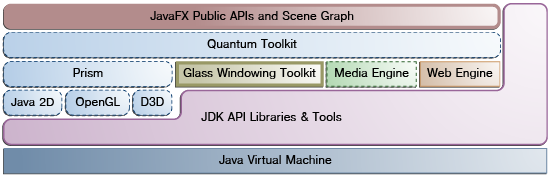
\includegraphics[width=0.75\linewidth]{image1.png}
  \\[4pt]{\small Слика 1. Дијаграм архитектуре JavaFX извршног окружења.}
\end{center}
\bigskip


\textbf{JavaFX Public API} – омогућава програмерима приступ функционалностима потребним за креирање компонената графичког корисничког интерфејса, анимација и других елемената. API је богат и укључује широк спектар класа и метода за рад са различитим аспектима графичких интерфејса.

\textbf{Граф сцене} (енг. \textit{Scene Graph}) – хијерархијска структура која обухвата све елементе графичких корисничких интерфејса у апликацији. Сваки елемент у графу сцене представља чвор (\texttt{Node}), а чворови могу имати потомке, формирајући дрволику структуру. Граф сцене омогућава ефикасно управљање великим бројем елемената, укључујући њихово позиционирање, трансформације и примену визуелних ефеката.

\textbf{Prism} – графички механизам који се користи за приказивање садржаја дефинисаног у графу сцене. Prism може користити софтверско приказивање или се ослонити на хардверско убрзање користећи DirectX (на Windows платформи) или OpenGL (на осталим платформама).

\textbf{Quantum Toolkit} – слој који повезује Prism са системским ресурсима. Управља нитима и догађајима приликом приказивања, осигуравајући да компоненте графичког корисничког интерфејса не блокирају главну нит апликације.

\textbf{Glass Window Toolkit} – компонента која служи као спрега између JavaFX апликација и оперативног система. Предвиђена је за управљање ресурсима као што су прозори и сесије.

\textbf{Media Engine} и \textbf{Web Engine} – компоненте које обезбеђују интеграцију мултимедијалних садржаја (аудио и видео) и уграђени прегледач веба у оквиру JavaFX апликација.


\subsection{JavaFX и FXML}

FXML је тип XML формата који се користи за дефинисање графичког корисничког интерфејса у JavaFX апликацијама. FXML користи XML за дефинисање елемената интерфејса декларативно, одвајајући изглед интерфејса од програмске логике апликације, слично начину на који се HTML користи за структурирање веб страница.

Елементи дефинисани у FXML-у директно се пресликавају на компоненте JavaFX-а, као што су дугмад, прозори и форме. Следећи пример показује једноставну FXML датотеку:


\needspace{5\baselineskip}
\begin{lstlisting}[language=Java]
<?xml version="1.0" encoding="UTF-8"?>
 
<?import javafx.scene.layout.VBox?>
<?import javafx.scene.control.Label?>
<?import javafx.scene.control.Button?>
 
<VBox spacing="10" alignment="CENTER"
   xmlns:fx="http://javafx.com/fxml">
   <Label text="Zdravo, FXML!" />
   <Button text="Klikni me"
         onAction="#obradiKlik" />
</VBox>
\end{lstlisting}


Контролери се у JavaFX-у користе за управљање интеракцијом са корисником, обрађујући догађаје који су дефинисани у FXML-у. FXML датотека се учитава у Јава коду помоћу класе \texttt{FXMLLoader}:


\needspace{5\baselineskip}
\begin{lstlisting}[language=Java]
// Учитавање FXML датотеке
FXMLLoader loader = new FXMLLoader(
   getClass().getResource("izgled.fxml"));
Parent koren = loader.load();
Scene scena = new Scene(koren, 400, 300);
\end{lstlisting}


FXML се такође може користити за повезивање компонената корисничког интерфејса са моделима података кроз механизме повезивања својстава и обраде догађаја, омогућавајући динамичко ажурирање интерфејса.


\subsection{JavaFX Scene Builder}

JavaFX Scene Builder је визуелни алат који користи FXML за дизајнирање компонената графичког корисничког интерфејса. Омогућава програмерима да лако приступе различитим компонентама JavaFX-а попут дугмади, текстуалних поља, листа, језичака и других контрола.

Програмери могу превлачењем компонената на радну површину брзо креирати сложене графичке корисничке интерфејсе без писања FXML кода ручно. Scene Builder генерише одговарајући FXML датотеку који се затим укључује у Јава пројекат.

Scene Builder укључује могућност измене фонтова, боја, маргина и многих других стилских аспеката применом CSS стилова на JavaFX компоненте директно унутар алата, чиме се омогућава прилагођавање изгледа апликације.


\subsection{Планиране карактеристике за нове верзије JavaFX}

С обзиром на значај JavaFX-а у развоју богатих графичких корисничких интерфејса и даље се ради на његовом развоју у оквиру OpenJFX пројекта. Неке од планираних карактеристика укључују додавање нових графичких компонената и побољшање постојећих.

У плану је да нове верзије JavaFX-а имају унапређене перформансе графичког приказивања ослањајући се на хардверско убрзање, уз проширење подршке за новије графичке API-је као што су Vulkan и DirectX 12.

Један од циљева у развоју нових верзија јесте стављање фокуса на облак (енг. \textit{cloud}) и мобилне платформе. С обзиром на развој облак технологија и мобилних уређаја, планира се унапређење подршке за покретање JavaFX апликација на различитим платформама, укључујући Android и iOS.

\section{Исцртавање код JavaFX}

\subsection{Покретање JavaFX апликације, класа Application}

Класа \texttt{Application} представља основну класу сваке JavaFX апликације. Она управља животним циклусом апликације: иницијализацијом, покретањем и заустављањем. Сваки JavaFX програм мора да наследи ову класу и имплементира метод \texttt{start()}.

Животни циклус JavaFX апликације састоји се од три фазе. Прво се позива метод \texttt{init()} који служи за иницијализацију ресурса (подразумевана имплементација је празна). Затим се позива метод \texttt{start(Stage primaryStage)} у коме се дефинише почетно графичко окружење апликације. На крају, при затварању апликације позива се метод \texttt{stop()} за ослобађање ресурса.


\bigskip

\noindent \textbf{Пример 1.} Основна структура JavaFX апликације. $\square$

\medskip

Следећи програм демонстрира минималну JavaFX апликацију која приказује прозор са текстом:


\needspace{5\baselineskip}
\begin{lstlisting}[language=Java]
package rs.math.oop.g05.p01.osnovnaAplikacija;
import javafx.application.Application;
import javafx.scene.Scene;
import javafx.scene.control.Label;
import javafx.scene.layout.StackPane;
import javafx.stage.Stage;
 
public class Primer01_OsnovnaAplikacija extends Application {
 
   @Override
   public void start(Stage primaryStage) {
         // Креирање ознаке и контејнера
         Label oznaka = new Label("Zdravo, JavaFX!");
         oznaka.setStyle("-fx-font-size: 24px;");
 
         StackPane koren = new StackPane();
         koren.getChildren().add(oznaka);
 
         // Креирање сцене и подешавање позорнице
         Scene scena = new Scene(koren, 400, 300);
 
         primaryStage.setTitle("Prva JavaFX aplikacija");
         primaryStage.setScene(scena);
         primaryStage.show();
   }
 
   public static void main(String[] args) {
         launch(args);
   }
}
\end{lstlisting}


Класа \texttt{Primer01\_OsnovnaAplikacija} наслеђује \texttt{Application} и имплементира метод \texttt{start()}. У методу \texttt{start()} креира се ознака (енг. \texttt{Label}), поставља се у контејнер \texttt{StackPane} (који центрира садржај), креира се сцена димензија 400x300 пиксела и постављају се наслов и сцена на примарну позорницу. Позив \texttt{primaryStage.show()} приказује прозор.


\subsection{Платформа, класа Platform}

Класа \texttt{javafx.application.Platform} садржи статичке методе за управљање извршним JavaFX окружењем, укључујући управљање нитима и животним циклусом апликације.

Метод \texttt{Platform.runLater(Runnable)} омогућава извршавање кода на JavaFX апликационој нити из друге нити. Ово је неопходно јер се сви елементи графичког корисничког интерфејса морају ажурирати искључиво из апликационе нити:


\needspace{5\baselineskip}
\begin{lstlisting}[language=Java]
// Ажурирање интерфејса из позадинске нити
Platform.runLater(() -> {
   oznaka.setText("Ucitavanje zavrseno!");
});
\end{lstlisting}


Метод \texttt{Platform.exit()} зауставља JavaFX апликацију и позива метод \texttt{stop()} пре затварања. Метод \texttt{Platform.isSupported(ConditionalFeature)} проверава да ли извршно окружење подржава одређену функционалност, као што је 3D графика или транспарентни прозори.


\subsection{Позорница, класа Stage}

Позорница (објекат класе \texttt{Stage}) је главни контејнер за све JavaFX сцене. Tо је прозор у коме се приказује садржај. Свака апликација добија једну примарну позорницу при покретању, а додатне позорнице могу се креирати за помоћне и искачуће (енг. \textit{pop-up}) прозоре.

Позорница нуди методе за подешавање наслова (\texttt{setTitle()}), димензија (\texttt{setWidth()}, \texttt{setHeight()}), минималних и максималних димензија, стила прозора (\texttt{initStyle()}) и модалности (\texttt{initModality()}). Стил прозора одређује да ли прозор има стандардне контроле (минимизација, максимизација, затварање) или је без декорације:


\needspace{5\baselineskip}
\begin{lstlisting}[language=Java]
// Креирање додатне позорнице
Stage noviProzor = new Stage();
noviProzor.setTitle("Pomocni prozor");
noviProzor.initModality(Modality.APPLICATION_MODAL);
noviProzor.setWidth(300);
noviProzor.setHeight(200);
noviProzor.show();
\end{lstlisting}


\subsection{Сцена, класа Scene}

Сцена (објекат класе \texttt{Scene}) је контејнер за све компоненте графичког корисничког интерфејса. Може се посматрати као корени чвор дрволике структуре у коју се слажу сви елементи интерфејса. Сцена се креира са коренским чвором и опционо са димензијама:


\needspace{5\baselineskip}
\begin{lstlisting}[language=Java]
VBox koren = new VBox();
Scene scena = new Scene(koren, 600, 400);
 
// Додавање CSS стилова на сцену
scena.getStylesheets().add("stil.css");
 
primaryStage.setScene(scena);
\end{lstlisting}


Сцена такође омогућава приступ својству за курсор (\texttt{setCursor()}), боју позадине (\texttt{setFill()}) и регистровање ослушкивача за догађаје тастатуре и миша на нивоу целе сцене.


\subsection{Елементи на сцени}

Сви елементи који се могу приказати на сцени наслеђују апстрактну класу \texttt{javafx.scene.Node}. Чвор је основна јединица графа сцене и може представљати контролу (дугме, поље за текст), облик (круг, правоугаоник), текст, слику или групу других чворова.

\subsubsection{Чвор, класа Node}

Класа \texttt{Node} дефинише заједничка својства за све елементе сцене: позицију (\texttt{layoutX}, \texttt{layoutY}), видљивост (\texttt{setVisible()}), прозирност (\texttt{setOpacity()}), трансформације (ротација, скалирање, транслација), ефекте и стил. Свaki чвор може имати јединствен идентификатор (\texttt{setId()}) и CSS класе (\texttt{getStyleClass()}).

\subsubsection{Група, класа Group}

Класа \texttt{Group} је контејнер који групише више елемената. За разлику од распореда (енг. \textit{layout}), група не примењује никакво позиционирање на своје потомке него они задржавају своје апсолутне координате. Група је корисна када је потребно применити исту трансформацију или ефекат на скуп елемената.

\subsubsection{Облик, класа Shape}

Апстрактна класа \texttt{Shape} из пакета \texttt{javafx.scene.shape} је базна класа за све геометријске облике. Дефинише заједничка својства: боју испуне (\texttt{setFill()}), боју и ширину ивице (\texttt{setStroke()}, \texttt{setStrokeWidth()}), стил ивице и друга визуелна својства. Сви конкретни облици као што су \texttt{Circle}, \texttt{Rectangle}, \texttt{Line} и \texttt{Polygon} наслеђују ову класу.

\subsubsection{Елипса и круг, класа Ellipse и класа Circle}

Класа \texttt{Ellipse} представља елипсу задату центром и полуосама, а класа \texttt{Circle} представља круг задат центром и полупречником. Круг је специјалан случај елипсе:


\needspace{5\baselineskip}
\begin{lstlisting}[language=Java]
// Креирање круга
Circle krug = new Circle(100, 100, 50);
krug.setFill(Color.BLUE);
krug.setStroke(Color.DARKBLUE);
krug.setStrokeWidth(2);
 
// Креирање елипсе
Ellipse elipsa = new Ellipse(300, 100, 80, 50);
elipsa.setFill(Color.CORAL);
\end{lstlisting}


За правоугаоник се користи класа \texttt{Rectangle} која подржава и заобљене углове помоћу својстава \texttt{setArcWidth()} и \texttt{setArcHeight()}. Класа \texttt{Line} представља праву линију, а класе \texttt{Polygon} и \texttt{Polyline} представљају многоугаоник и отворену полилинију.


\needspace{5\baselineskip}
\begin{lstlisting}[language=Java]
// Правоугаоник са заобљеним угловима
Rectangle pravougaonik = new Rectangle(200, 50, 150, 100);
pravougaonik.setFill(Color.LIGHTGREEN);
pravougaonik.setArcWidth(15);
pravougaonik.setArcHeight(15);
\end{lstlisting}


\subsubsection{Текст, класа Text}

Класа \texttt{Text} омогућава исцртавање текста на сцени. За разлику од класе \texttt{Label} (која је контрола), \texttt{Text} је облик и нуди детаљнију контролу над положајем и изгледом текста:


\needspace{5\baselineskip}
\begin{lstlisting}[language=Java]
Text tekst = new Text(50, 100, "Zdravo, svete!");
tekst.setFont(Font.font("Arial", FontWeight.BOLD, 24));
tekst.setFill(Color.DARKRED);
\end{lstlisting}


\subsubsection{Крива}

За цртање кривих линија JavaFX нуди класе \texttt{QuadCurve} (квадратна Безијеова крива са једном контролном тачком) и \texttt{CubicCurve} (кубна Безијеова крива са две контролне тачке). Контролне тачке одређују облик кривине:


\needspace{5\baselineskip}
\begin{lstlisting}[language=Java]
// Кубна Безијеова крива
CubicCurve kriva = new CubicCurve();
kriva.setStartX(50);   kriva.setStartY(200);
kriva.setControlX1(150); kriva.setControlY1(20);
kriva.setControlX2(300); kriva.setControlY2(20);
kriva.setEndX(400);    kriva.setEndY(200);
kriva.setStroke(Color.DARKBLUE);
kriva.setFill(Color.TRANSPARENT);
\end{lstlisting}


За сложеније облике користи се класа \texttt{Path} која представља путању састављену од сегмената: \texttt{MoveTo} (почетна тачка), \texttt{LineTo} (линија), \texttt{ArcTo} (лук), \texttt{QuadCurveTo} и \texttt{CubicCurveTo} (криве) и \texttt{ClosePath} (затварање путање).


\subsection{Ефекти при исцртавању}

JavaFX омогућава додавање различитих визуелних ефеката на чворове графа сцене. Ефекти се примењују позивом метода \texttt{setEffect()} на било ком чвору. Најчешће коришћени ефекти налазе се у пакету \texttt{javafx.scene.effect}:

\texttt{DropShadow} – додаје сенку иза елемента. Подешава се положај сенке, полупречник замућења и боја.

\texttt{InnerShadow} – додаје унутрашњу сенку, стварајући ефекат удубљења.

\texttt{GaussianBlur} – примењује Гаусово замућење на елемент.

\texttt{Reflection} – додаје одраз испод елемента.

\texttt{Glow} – додаје ефекат сијања око елемента.


\needspace{5\baselineskip}
\begin{lstlisting}[language=Java]
// Примена сенке и замућења
DropShadow senka = new DropShadow();
senka.setOffsetX(5);
senka.setOffsetY(5);
senka.setColor(Color.GRAY);
 
Label oznaka = new Label("Tekst sa senkom");
oznaka.setEffect(senka);
 
Rectangle pravougaonik = new Rectangle(100, 60);
pravougaonik.setEffect(new GaussianBlur(10));
\end{lstlisting}


Ефекти се могу и комбиновати повезивањем у ланац. Сваки ефекат има својство \texttt{setInput()} које прима други ефекат као улаз.


\subsection{Трансформације}

Трансформације омогућавају измене позиција, величина и ротација елемената на сцени. JavaFX подржава следеће трансформације из пакета \texttt{javafx.scene.transform}:

\texttt{Translate} – помера елемент за задати износ по X и Y оси.

\texttt{Rotate} – ротира елемент око задате тачке за одређени угао.

\texttt{Scale} – мења величину елемента по X и Y оси.

\texttt{Shear} – примењује смицање (нагињање) елемента.

Трансформације се могу применити на два начина – директно кроз својства чвора или додавањем у листу трансформација:


\needspace{5\baselineskip}
\begin{lstlisting}[language=Java]
// Директно кроз својства чвора
Rectangle r1 = new Rectangle(50, 50);
r1.setRotate(45);            // Ротација за 45 степени
r1.setScaleX(1.5);           // Увећање по X оси
r1.setTranslateX(100);       // Померање по X оси
 
// Коришћењем листе трансформација
Rectangle r2 = new Rectangle(50, 50);
r2.getTransforms().addAll(
   new Rotate(30, 25, 25),   // Ротација око центра
   new Scale(2, 2),          // Двоструко увећање
   new Translate(50, 50)     // Померање
);
\end{lstlisting}


\subsection{Распореди}

JavaFX нуди више контејнерских класа за распоређивање чворова унутар сцене. Свака класа за распоред (енг. \textit{layout}) дефинише правила по којима се чворови позиционирају. Најчешће коришћени распореди су:

\texttt{VBox} – распоређује чворове вертикално, један испод другог. Размак између чворова подешава се методом \texttt{setSpacing()}.

\texttt{HBox} – распоређује чворове хоризонтално, један поред другог.

\texttt{BorderPane} – дели простор на пет области: горњу, доњу, леву, десну и централну. Погодан за стандардни распоред апликације са траком менија, бочним панелом и централним садржајем.

\texttt{GridPane} – распоређује чворове у мрежу (табелу) са редовима и колонама. Сваки чвор се поставља на одређену позицију помоћу метода \texttt{add(node, column, row)}.

\texttt{StackPane} – поставља чворове једне преко других, центриране. Користи се за прекривање елемената.

\texttt{FlowPane} – распоређује чворове у ред и прелази у нови ред када нема више простора. Слично распореду текста у параграфу.


\bigskip

\noindent \textbf{Пример 2.} Распореди и контроле. $\square$

\medskip

Следећи програм демонстрира коришћење распореда \texttt{VBox}, \texttt{HBox} и \texttt{GridPane} заједно са основним контролама:


\needspace{5\baselineskip}
\begin{lstlisting}[language=Java]
package rs.math.oop.g05.p02.rasporediIKontrole;
import javafx.application.Application;
import javafx.geometry.Insets;
import javafx.geometry.Pos;
import javafx.scene.Scene;
import javafx.scene.control.*;
import javafx.scene.layout.*;
import javafx.stage.Stage;
 
public class Primer02_RasporediIKontrole extends Application {
 
   @Override
   public void start(Stage primaryStage) {
         // Горњи део - HBox са дугмадима
         Button dugmeNovo = new Button("Novo");
         Button dugmeSacuvaj = new Button("Sacuvaj");
         Button dugmeObrisi = new Button("Obrisi");
 
         HBox traka = new HBox(10, dugmeNovo, dugmeSacuvaj,
          dugmeObrisi);
         traka.setPadding(new Insets(10));
         traka.setAlignment(Pos.CENTER_LEFT);
 
         // Централни део - GridPane са формом
         GridPane forma = new GridPane();
         forma.setHgap(10);
         forma.setVgap(10);
         forma.setPadding(new Insets(20));
 
         forma.add(new Label("Ime:"), 0, 0);
         forma.add(new TextField(), 1, 0);
         forma.add(new Label("Prezime:"), 0, 1);
         forma.add(new TextField(), 1, 1);
         forma.add(new Label("Email:"), 0, 2);
         forma.add(new TextField(), 1, 2);
 
         CheckBox aktivan = new CheckBox("Aktivan korisnik");
         forma.add(aktivan, 1, 3);
 
         // Доњи део - HBox са статусом
         Label status = new Label("Spremno.");
         HBox statusTraka = new HBox(status);
         statusTraka.setPadding(new Insets(5, 10, 5, 10));
 
         // BorderPane као главни распоред
         BorderPane glavni = new BorderPane();
         glavni.setTop(traka);
         glavni.setCenter(forma);
         glavni.setBottom(statusTraka);
 
         Scene scena = new Scene(glavni, 450, 300);
 
         primaryStage.setTitle("Forma sa rasporedom");
         primaryStage.setScene(scena);
         primaryStage.show();
   }
 
   public static void main(String[] args) {
         launch(args);
   }
}
\end{lstlisting}


Овај пример комбинује три распореда. \texttt{BorderPane} дели прозор на горњу траку са дугмадима (\texttt{HBox}), централну форму (\texttt{GridPane}) и доњу статусну линију. У \texttt{GridPane} елементи се постављају по колонама и редовима, па су ознаке и поља за унос поравнати. Класа \texttt{Insets} дефинише унутрашњу маргину контејнера.


\section{Једноставне контроле код JavaFX}

JavaFX садржи богат скуп контрола за интеракцију са корисником. Све контроле наслеђују класу \texttt{javafx.scene.control.Control} која наслеђује \texttt{Node}. У овом одељку приказане су најчешће коришћене контроле.


\subsection{Дугме}

Класа \texttt{Button} представља дугме на које корисник може да кликне. Догађај клика обрађује се помоћу метода \texttt{setOnAction()} који прима ослушкивач типа \texttt{EventHandler\textless{}ActionEvent\textgreater{}}. Од Јаве 8, ослушкивач се најчешће задаје као ламбда израз:


\needspace{5\baselineskip}
\begin{lstlisting}[language=Java]
Button dugme = new Button("Klikni me");
dugme.setOnAction(event -> {
   System.out.println("Dugme je kliknuto!");
});
\end{lstlisting}


Текст дугмета може се мењати методом \texttt{setText()}, а стање (омогућено/онемогућено) методом \texttt{setDisable()}.


\subsection{Текстуално поље}

Класа \texttt{TextField} представља поље за унос текста у једном реду. Текст се чита методом \texttt{getText()} и поставља методом \texttt{setText()}. За ослушкивање промена текста користи се метод \texttt{textProperty()} који враћа одговарајуће својство (видети одељак 5.4).

За унос текста у више редова користи се класа \texttt{TextArea}.


\subsection{Ознака}

Класа \texttt{Label} приказује текст који корисник не може да мења. Ознаке се користе за описе поља у формама, приказ информација и статусне поруке. Стил текста може се подесити помоћу CSS–а кроз метод \texttt{setStyle()} или постављањем фонта кроз \texttt{setFont()}.


\subsection{Поље за потврду}

Класа \texttt{CheckBox} представља поље за потврду које може бити означено или неозначено. Стање се чита методом \texttt{isSelected()} и поставља методом \texttt{setSelected()}. Промена стања може се ослушкивати кроз метод \texttt{selectedProperty()} који враћа одговарајуће својство.


\subsection{Мени}

JavaFX подржава систем менија преко класа \texttt{MenuBar}, \texttt{Menu} и \texttt{MenuItem}. Линија менија (енг. \texttt{MenuBar}) садржи један или више менија, а сваки мени садржи ставке. Ставке менија могу имати пречице на тастатури и обраде догађаја:


\needspace{5\baselineskip}
\begin{lstlisting}[language=Java]
MenuBar linijaMenija = new MenuBar();
 
Menu datoteka = new Menu("Datoteka");
MenuItem novo = new MenuItem("Novo");
novo.setOnAction(e -> System.out.println("Novo"));
MenuItem sacuvaj = new MenuItem("Sacuvaj");
MenuItem izadji = new MenuItem("Izadji");
izadji.setOnAction(e -> Platform.exit());
 
datoteka.getItems().addAll(novo, sacuvaj,
   new SeparatorMenuItem(), izadji);
linijaMenija.getMenus().add(datoteka);
\end{lstlisting}


Класа \texttt{SeparatorMenuItem} додаје визуелну линију раздвајања између ставки менија. За пречице на тастатури користи се метод \texttt{setAccelerator()} са објектом класе \texttt{KeyCombination}.


\subsection{CSS стилизација}

Једна од значајних предности JavaFX у односу на Swing јесте могућност стилизације корисничког интерфејса помоћу CSS–а (\textit{Cascading Style Sheets}). Свако JavaFX својство за стилизацију почиње префиксом \texttt{-fx-} како би се разликовало од стандардних CSS својстава за веб.

Стил се може задати директно на појединачном чвору помоћу метода \texttt{setStyle()}:


\needspace{5\baselineskip}
\begin{lstlisting}[language=Java]
// Инлајн стилизација појединачног чвора
Label oznaka = new Label("Naslov");
oznaka.setStyle("-fx-font-size: 20px; "
   + "-fx-font-weight: bold; "
   + "-fx-text-fill: #336699;");
\end{lstlisting}


За сложеније апликације препоручује се коришћење спољашњих CSS датотека. Датотека стилова додаје се на сцену позивом метода \texttt{getStylesheets().add()}:


\needspace{5\baselineskip}
\begin{lstlisting}[language=Java]
// Учитавање стилова из спољашњег фајла
Scene scena = new Scene(koren, 400, 300);
scena.getStylesheets().add(
   getClass().getResource("stil.css")
         .toExternalForm());
\end{lstlisting}


Пример садржаја CSS датотеке за JavaFX:


\needspace{5\baselineskip}
\begin{lstlisting}[language=Java]
/* stil.css */
.label {
   -fx-font-family: "Arial";
   -fx-font-size: 14px;
}
 
.button {
   -fx-background-color: #4CAF50;
   -fx-text-fill: white;
   -fx-padding: 8px 16px;
   -fx-cursor: hand;
}
 
.button:hover {
   -fx-background-color: #45a049;
}
\end{lstlisting}


Поред подразумеваних CSS класа које JavaFX додељује контролама (нпр. \texttt{.label}, \texttt{.button}, \texttt{.text-field}), програмер може да додели произвољну CSS класу помоћу метода \texttt{getStyleClass().add()} или да постави јединствен идентификатор помоћу метода \texttt{setId()} и примени стил кроз селектор \texttt{\#id}.


\bigskip

\noindent \textbf{Пример 3.} Контроле и обрада догађаја. $\square$

\medskip

Следећи програм демонстрира коришћење различитих контрола са обрадом догађаја:


\needspace{5\baselineskip}
\begin{lstlisting}[language=Java]
package rs.math.oop.g05.p03.kontrole;
import javafx.application.Application;
import javafx.geometry.Insets;
import javafx.scene.Scene;
import javafx.scene.control.*;
import javafx.scene.layout.VBox;
import javafx.stage.Stage;
 
public class Primer03_Kontrole extends Application {
 
   @Override
   public void start(Stage primaryStage) {
         // Креирање контрола за форму
         Label naslov = new Label("Registracija");
         naslov.setStyle("-fx-font-size: 18px; "
          + "-fx-font-weight: bold;");
 
         TextField imePolje = new TextField();
         imePolje.setPromptText("Unesite ime");
 
         PasswordField lozinkaPolje = new PasswordField();
         lozinkaPolje.setPromptText("Unesite lozinku");
 
         CheckBox usloviPolje = new CheckBox(
          "Prihvatam uslove koriscenja");
 
         Button registrujSe = new Button("Registruj se");
         Label poruka = new Label();
 
         // Обрада догађаја клика на дугме
         registrujSe.setOnAction(event -> {
          String ime = imePolje.getText();
          boolean uslovi = usloviPolje.isSelected();
 
          if (ime.isEmpty()) {
                poruka.setText("Unesite ime!");
                poruka.setStyle("-fx-text-fill: red;");
          } else if (!uslovi) {
                poruka.setText("Morate prihvatiti uslove.");
                poruka.setStyle("-fx-text-fill: red;");
          } else {
                poruka.setText("Dobrodosli, " + ime + "!");
                poruka.setStyle("-fx-text-fill: green;");
          }
         });
 
         // Вертикални распоред са размаком од 10 пиксела
         VBox koren = new VBox(10, naslov, imePolje,
          lozinkaPolje, usloviPolje, registrujSe, poruka);
         koren.setPadding(new Insets(20));
 
         Scene scena = new Scene(koren, 350, 300);
         primaryStage.setTitle("Registracija");
         primaryStage.setScene(scena);
         primaryStage.show();
   }
 
   public static void main(String[] args) {
         launch(args);
   }
}
\end{lstlisting}


У овом примеру, \texttt{VBox} распоређује контроле вертикално. Приликом клика на дугме, програм проверава да ли је корисник унео име и прихватио услове. Класа \texttt{PasswordField} наслеђује \texttt{TextField} и приказује маскиране карактере уместо стварног текста. Метод \texttt{setPromptText()} поставља текст који се приказује као сугестија када је поље празно.


\section{Особине, догађаји и повезивање код JavaFX}

Једна од кључних разлика JavaFX у односу на Swing јесте систем својстава (енг. \textit{properties}) и повезивања (енг. \textit{binding}). Овај систем омогућава аутоматску синхронизацију вредности између различитих елемената интерфејса без потребе за ручним ажурирањем.


\subsection{Особине}

Свако JavaFX својство је објекат који обавија (енг. \textit{wraps}) неку вредност и подржава ослушкивање промена. За основне типове постоје одговарајуће класе својстава: \texttt{SimpleStringProperty}, \texttt{SimpleIntegerProperty}, \texttt{SimpleDoubleProperty}, \texttt{SimpleBooleanProperty} и друге. Свака од ових класа нуди три кључна метода:

\texttt{get()} и \texttt{set()} – узимање и постављање вредности својства.

\texttt{addListener()} – регистровање ослушкивача који се позива при свакој промени вредности.

\texttt{bind()} и \texttt{bindBidirectional()} – повезивање са другим својством (једносмерно или двосмерно).

\subsubsection{Класе за особине}

JavaFX разликује два типа ослушкивача за својства. \texttt{InvalidationListener} се позива када вредност својства постане невалидна (тј. када се промени, али пре него што се нова вредност израчуна). \texttt{ChangeListener} се позива након промене и добија стару и нову вредност:


\needspace{5\baselineskip}
\begin{lstlisting}[language=Java]
StringProperty ime = new SimpleStringProperty("Marko");
 
// Ослушкивање промене
ime.addListener((observable, staraVrednost, novaVrednost) -> {
   System.out.println("Ime promenjeno: "
         + staraVrednost + " -> " + novaVrednost);
});
 
ime.set("Petar");  // Исписује: Ime promenjeno: Marko -> Petar
\end{lstlisting}


Све контроле у JavaFX омогућавају приступ својим особинама као својствима. На пример, класа \texttt{TextField} нуди метод \texttt{textProperty()} који враћа својство текста, а класа \texttt{CheckBox} нуди метод \texttt{selectedProperty()} који враћа својство означености. Ово омогућава директно ослушкивање и повезивање контрола.


\subsection{Једносмерно и двосмерно повезивање}

Повезивање (енг. \textit{binding}) омогућава да вредност једног својства аутоматски прати вредност другог. Постоје две врсте повезивања:

\textbf{Једносмерно повезивање} – једно својство прати вредност другог. Када се извор промени, повезано својство се аутоматски ажурира. Подешава се позивом \texttt{bind()}. Након повезивања, вредност повезаног својства не може се ручно мењати.

\textbf{Двосмерно повезивање} – оба својства прате једно друго. Промена било ког од њих ажурира друго. Подешава се позивом \texttt{bindBidirectional()}.

\subsubsection{Класе и интерфејси за реализацију повезивања}

Повезивање се може комбиновати са аритметичким операцијама и логичким условима:


\needspace{5\baselineskip}
\begin{lstlisting}[language=Java]
DoubleProperty sirina = new SimpleDoubleProperty(10);
DoubleProperty visina = new SimpleDoubleProperty(20);
 
// Површина се аутоматски ажурира када се промени
// ширина или висина
NumberBinding povrsina = sirina.multiply(visina);
 
System.out.println(povrsina.getValue()); // 200.0
sirina.set(15);
System.out.println(povrsina.getValue()); // 300.0
\end{lstlisting}


Класа \texttt{Bindings} нуди статичке методе за сложеније изразе повезивања, као што су \texttt{Bindings.when()} (условно повезивање), \texttt{Bindings.format()} (форматирање текста) и \texttt{Bindings.concat()} (спајање стрингова).

\subsubsection{Повезивање са JavaFX зрнима}

JavaFX зрна (енг. \textit{beans}) су класе које следе конвенцију дефинисања својстава тако да за свако својство постоје три метода: метод за узимање вредности (нпр. \texttt{getIme()}), метод за постављање вредности (нпр. \texttt{setIme()}) и метод који враћа објекат својства (нпр. \texttt{imeProperty()}). Ова конвенција омогућава аутоматско повезивање са контролама попут \texttt{TableView}.


\bigskip

\noindent \textbf{Пример 4.} Својства и повезивање. $\square$

\medskip

Следећи програм демонстрира повезивање својстава JavaFX контрола:


\needspace{5\baselineskip}
\begin{lstlisting}[language=Java]
package rs.math.oop.g05.p04.povezivanje;
import javafx.application.Application;
import javafx.beans.binding.Bindings;
import javafx.geometry.Insets;
import javafx.scene.Scene;
import javafx.scene.control.*;
import javafx.scene.layout.VBox;
import javafx.stage.Stage;
 
public class Primer04_Povezivanje extends Application {
 
   @Override
   public void start(Stage primaryStage) {
         TextField imePolje = new TextField();
         imePolje.setPromptText("Unesite ime");
 
         Label pozdrav = new Label();
         // Једносмерно повезивање: поздрав прати име
         pozdrav.textProperty().bind(
          Bindings.concat("Zdravo, ",
                imePolje.textProperty(), "!"));
 
         Slider velicinaSlajder = new Slider(10, 40, 20);
         velicinaSlajder.setShowTickLabels(true);
 
         // Повезивање величине фонта са клизачем
         pozdrav.styleProperty().bind(
          Bindings.concat("-fx-font-size: ",
                velicinaSlajder.valueProperty()
                .asString("%.0f"),
                "px;"));
 
         CheckBox vidljivPolje = new CheckBox("Prikazi pozdrav");
         vidljivPolje.setSelected(true);
 
         // Повезивање видљивости
         pozdrav.visibleProperty().bind(
          vidljivPolje.selectedProperty());
 
         VBox koren = new VBox(15, imePolje,
          velicinaSlajder, vidljivPolje, pozdrav);
         koren.setPadding(new Insets(20));
 
         Scene scena = new Scene(koren, 400, 250);
         primaryStage.setTitle("Povezivanje svojstava");
         primaryStage.setScene(scena);
         primaryStage.show();
   }
 
   public static void main(String[] args) {
         launch(args);
   }
}
\end{lstlisting}


У овом примеру, текст ознаке \texttt{pozdrav} аутоматски се ажурира док корисник куца у текстуално поље. Величина фонта ознаке повезана је са вредношћу клизача (енг. \texttt{Slider}), а видљивост ознаке повезана је са стањем поља за потврду. Ниједна обрада догађаја није ручно написана већ сва ажурирања обавља систем повезивања.


\subsection{Догађаји}

Обрада догађаја у JavaFX заснива се на концептима описаним у поглављу 4, примењеним на граф сцене. Сваки чвор може да региструје ослушкиваче за различите типове догађаја: \texttt{ActionEvent} (клик на дугме), \texttt{MouseEvent} (миш), \texttt{KeyEvent} (тастатура), \texttt{ScrollEvent} (точкић миша) и друге.

\subsubsection{Класе и методи за ослушкивање догађаја}

Догађај у JavaFX пролази кроз две фазе:

\textbf{Фаза хватања} (енг. \textit{capturing}) – догађај се прослеђује од корена графа сцене ка циљном чвору. Сваки чвор на путањи може да региструје филтер помоћу метода \texttt{addEventFilter()}.

\textbf{Фаза пропагације} (енг. \textit{bubbling}) – догађај се враћа од циљног чвора ка корену. Обрада се региструје помоћу метода \texttt{addEventHandler()} или пречица попут \texttt{setOnMouseClicked()}.

Чвор може да заустави даљу пропагацију позивом \texttt{event.consume()}.

\subsubsection{Коришћење повезивања ради поравнавања елемената}

Повезивање се може користити и за динамичко позиционирање елемената. На пример, центрирање елемента на сцени може се остварити повезивањем његове позиције са димензијама сцене:


\needspace{5\baselineskip}
\begin{lstlisting}[language=Java]
// Центрирање круга на сцени
Circle krug = new Circle(30, Color.RED);
krug.centerXProperty().bind(
   scena.widthProperty().divide(2));
krug.centerYProperty().bind(
   scena.heightProperty().divide(2));
\end{lstlisting}


На овај начин, круг ће увек остати центриран чак и када корисник промени величину прозора.


\section{Сложеније JavaFX компоненте}

Поред основних контрола описаних у одељку 5.3, JavaFX нуди сложеније компоненте за организацију садржаја и приказ структурираних података.


\subsection{Мени – напредне могућности}

Поред основног менија описаног у одељку 5.3.5, JavaFX подржава и напредније варијанте. Класа \texttt{RadioMenuItem} омогућава креирање ставки за избор једне опције из групе (слично радио-дугмадима). Класа \texttt{CheckMenuItem} додаје ставку менија са пољем за потврду. Контекстни мени (\texttt{ContextMenu}) приказује се десним кликом миша на неки елемент:


\needspace{5\baselineskip}
\begin{lstlisting}[language=Java]
// Контекстни мени
ContextMenu kontekstMeni = new ContextMenu();
MenuItem kopiraj = new MenuItem("Kopiraj");
MenuItem nalepii = new MenuItem("Nalepi");
kontekstMeni.getItems().addAll(kopiraj, nalepii);
 
tekstPolje.setContextMenu(kontekstMeni);
\end{lstlisting}


\subsection{Радио-дугме}

Класа \texttt{RadioButton} представља радио-дугме, контролу за избор једне опције из групе. Радио-дугмад се групишу помоћу класе \texttt{ToggleGroup}. Унутар једне групе само једно радио-дугме може бити означено у истом тренутку:


\needspace{5\baselineskip}
\begin{lstlisting}[language=Java]
ToggleGroup grupa = new ToggleGroup();
 
RadioButton rb1 = new RadioButton("Opcija A");
rb1.setToggleGroup(grupa);
rb1.setSelected(true);
 
RadioButton rb2 = new RadioButton("Opcija B");
rb2.setToggleGroup(grupa);
 
RadioButton rb3 = new RadioButton("Opcija C");
rb3.setToggleGroup(grupa);
 
// Ослушкивање промене избора
grupa.selectedToggleProperty().addListener(
   (obs, stari, novi) -> {
         if (novi != null) {
          RadioButton izabrano = (RadioButton) novi;
          System.out.println("Izabrano: "
                + izabrano.getText());
         }
   });
\end{lstlisting}


\subsection{Оквир за групу}

JavaFX нуди класу \texttt{TitledPane} која приказује садржај унутар оквира са насловом. Овај оквир може бити склопив. Корисник може да сакрије или прикаже садржај кликом на наслов. За груписање више \texttt{TitledPane} елемената користи се класа \texttt{Accordion}, која обезбеђује да само један оквир буде проширен у истом тренутку:


\needspace{5\baselineskip}
\begin{lstlisting}[language=Java]
// Оквир за групу са садржајем
TitledPane licniPodaci = new TitledPane(
   "Licni podaci",
   new VBox(10,
         new Label("Ime:"), new TextField(),
         new Label("Prezime:"), new TextField()));
 
TitledPane kontakt = new TitledPane(
   "Kontakt",
   new VBox(10,
         new Label("Email:"), new TextField(),
         new Label("Telefon:"), new TextField()));
 
Accordion harmonika = new Accordion(
   licniPodaci, kontakt);
harmonika.setExpandedPane(licniPodaci);
\end{lstlisting}


\subsection{Напредно поље за потврду}

Класа \texttt{CheckBox} подржава и треће, неодређено (енг. \textit{indeterminate}), стање. Ово стање је корисно када се поље за потврду односи на групу опција од којих су само неке означене. Треће стање се омогућава позивом \texttt{setAllowIndeterminate(true)} и проверава методом \texttt{isIndeterminate()}.


\subsection{Листа}

Класа \texttt{ListView} приказује листу елемената са могућношћу избора. Елементи се додају у \texttt{ObservableList} који аутоматски обавештава контролу о променама:


\needspace{5\baselineskip}
\begin{lstlisting}[language=Java]
ObservableList<String> stavke =
   FXCollections.observableArrayList(
         "Java", "Python", "C++", "JavaScript");
ListView<String> lista = new ListView<>(stavke);
 
// Ослушкивање избора
lista.getSelectionModel().selectedItemProperty()
   .addListener((obs, stari, novi) -> {
         System.out.println("Izabrano: " + novi);
   });
\end{lstlisting}


\subsection{Комбинована листа}

Класа \texttt{ComboBox} комбинује текстуално поље са падајућом листом. Корисник може да изабере ставку из листе или да откуца вредност ако је то дозвољено помоћу \texttt{setEditable(true)}:


\needspace{5\baselineskip}
\begin{lstlisting}[language=Java]
ComboBox<String> combo = new ComboBox<>();
combo.getItems().addAll(
   "Beograd", "Novi Sad", "Nis", "Kragujevac");
combo.setPromptText("Izaberite grad");
 
// Ослушкивање избора
combo.setOnAction(e ->
   System.out.println("Grad: "
         + combo.getValue()));
\end{lstlisting}


\subsection{Језичак}

Класа \texttt{TabPane} приказује садржај организован у језичке (енг. \textit{tabs}). Сваки језичак представља објекат класе \texttt{Tab} са насловом и садржајем:


\needspace{5\baselineskip}
\begin{lstlisting}[language=Java]
TabPane jezicciPanel = new TabPane();
 
Tab tab1 = new Tab("Podaci");
tab1.setContent(formaPanel);
tab1.setClosable(false);
 
Tab tab2 = new Tab("Statistika");
tab2.setContent(statistikaPanel);
 
jezicciPanel.getTabs().addAll(tab1, tab2);
\end{lstlisting}


\subsection{Табела}

Класа \texttt{TableView} приказује податке у облику табеле. Колоне се дефинишу помоћу класе \texttt{TableColumn} и повезују са својствима објеката података. JavaFX користи систем својстава за аутоматско ажурирање табеле када се подаци промене:


\needspace{5\baselineskip}
\begin{lstlisting}[language=Java]
TableView<Student> tabela = new TableView<>();
 
TableColumn<Student, String> kolIme =
   new TableColumn<>("Ime");
kolIme.setCellValueFactory(
   new PropertyValueFactory<>("ime"));
 
TableColumn<Student, Double> kolProsek =
   new TableColumn<>("Prosek");
kolProsek.setCellValueFactory(
   new PropertyValueFactory<>("prosek"));
 
tabela.getColumns().addAll(kolIme, kolProsek);
tabela.setItems(podaci);
\end{lstlisting}


Класа \texttt{PropertyValueFactory} повезује колону са JavaFX својством објекта. За класу \texttt{Student} то значи да мора имати методе \texttt{imeProperty()} и \texttt{prosekProperty()} које враћају одговарајућа JavaFX својства.


\section{Слике и анимација код JavaFX}

\subsection{Рад са сликама}

JavaFX пружа подршку за учитавање и приказивање слика кроз класе \texttt{Image} и \texttt{ImageView} из пакета \texttt{javafx.scene.image}.

\subsubsection{Класа Image}

Класа \texttt{Image} учитава слику из датотеке, URL адресе или тока података. Подржани формати укључују PNG, JPEG, GIF и BMP. Слика се може учитати синхроно или асинхроно (у позадини):


\needspace{5\baselineskip}
\begin{lstlisting}[language=Java]
// Учитавање слике из ресурса
Image slika = new Image("datoteka:slika.png");
 
// Асинхроно учитавање са задатим димензијама
Image velSlika = new Image("http://primer.rs/foto.jpg",
   200, 150,   // ширина, висина
   true,        // очувати однос страница
   true);       // учитати у позадини
\end{lstlisting}


\subsubsection{Класа ImageView}

Класа \texttt{ImageView} је чвор који приказује објекат класе \texttt{Image} на сцени. Омогућава подешавање величине приказа, ротацију и примену ефеката:


\needspace{5\baselineskip}
\begin{lstlisting}[language=Java]
Image slika = new Image("logo.png");
ImageView prikaz = new ImageView(slika);
 
// Подешавање величине приказа
prikaz.setFitWidth(200);
prikaz.setPreserveRatio(true);
 
// Заобљени углови
Rectangle clip = new Rectangle(200, 150);
clip.setArcWidth(20);
clip.setArcHeight(20);
prikaz.setClip(clip);
\end{lstlisting}


\subsection{Анимације}

JavaFX нуди уграђену подршку за анимације кроз класу \texttt{javafx.animation.Timeline}. Анимација се дефинише као низ кључних оквира (\texttt{KeyFrame}), од којих сваки описује стање у одређеном тренутку. JavaFX аутоматски интерполира вредности између кључних оквира.

\subsubsection{Класа Timeline}

Класа \texttt{Timeline} је основна класа за креирање анимација у JavaFX. Анимација се дефинише додавањем кључних оквира у временску линију. \texttt{Timeline} подржава понављање, аутоматско враћање уназад и различите брзине репродукције.

\subsubsection{Класе KeyFrame и KeyValue}

Класа \texttt{KeyFrame} прима трајање (\texttt{Duration}) и једну или више кључних вредности (\texttt{KeyValue}). Кључна вредност описује циљну вредност неког својства у том тренутку:


\needspace{5\baselineskip}
\begin{lstlisting}[language=Java]
// Анимација која помера круг са x=0 на x=300
// у трајању од 2 секунде
Circle krug = new Circle(20, Color.BLUE);
 
Timeline animacija = new Timeline(
   new KeyFrame(Duration.ZERO,
         new KeyValue(krug.translateXProperty(), 0)),
   new KeyFrame(Duration.seconds(2),
         new KeyValue(krug.translateXProperty(), 300))
);
 
animacija.setCycleCount(Timeline.INDEFINITE);
animacija.setAutoReverse(true);
animacija.play();
\end{lstlisting}


Метод \texttt{setCycleCount()} одређује колико пута се анимација понавља. Вредност \texttt{Timeline.INDEFINITE} значи бесконачно понављање. Метод \texttt{setAutoReverse(true)} чини да се анимација враћа уназад по завршетку сваког циклуса.

\subsubsection{Преласци код анимација}

Поред ручног дефинисања анимација преко кључних оквира, JavaFX нуди готове прелазе:

\texttt{FadeTransition} – постепено појављивање или нестајање елемента.

\texttt{TranslateTransition} – померање елемента.

\texttt{RotateTransition} – ротирање елемента.

\texttt{ScaleTransition} – промена величине елемента.

\texttt{PathTransition} – кретање елемента дуж задате путање.

\subsubsection{Повезивање и анимација}

Систем повезивања може се комбиновати са анимацијама. На пример, положај елемента може се повезати са вредношћу клизача, а анимација може да контролише вредност својства која се затим прослеђује кроз ланац повезивања. Такође, стање анимације (\texttt{Animation.Status}) може се користити за повезивање са контролама. На пример, дугме може да се онемогући док анимација траје.


\bigskip

\noindent \textbf{Пример 5.} Анимација и графика. $\square$

\medskip

Следећи програм демонстрира анимацију кругова који се крећу по екрану:


\needspace{5\baselineskip}
\begin{lstlisting}[language=Java]
package rs.math.oop.g05.p05.animacija;
import javafx.animation.*;
import javafx.application.Application;
import javafx.scene.Scene;
import javafx.scene.layout.Pane;
import javafx.scene.paint.Color;
import javafx.scene.shape.Circle;
import javafx.stage.Stage;
import javafx.util.Duration;
 
public class Primer05_Animacija extends Application {
 
   @Override
   public void start(Stage primaryStage) {
         Pane koren = new Pane();
 
         // Креирање кругова са анимацијом
         for (int i = 0; i < 5; i++) {
          Circle krug = new Circle(15 + i * 5);
          krug.setFill(Color.hsb(i * 60, 0.8, 0.9));
          krug.setCenterX(50 + i * 70);
          krug.setCenterY(150);
 
          // Вертикална анимација
          TranslateTransition tt =
                new TranslateTransition(
                Duration.seconds(1 + i * 0.3), krug);
          tt.setByY(-100 + i * 10);
          tt.setCycleCount(Animation.INDEFINITE);
          tt.setAutoReverse(true);
 
          // Ротација
          RotateTransition rt =
                new RotateTransition(
                Duration.seconds(2), krug);
          rt.setByAngle(360);
          rt.setCycleCount(Animation.INDEFINITE);
 
          // Промена величине
          ScaleTransition st =
                new ScaleTransition(
                Duration.seconds(1.5 + i * 0.2),
                krug);
          st.setToX(1.5);
          st.setToY(1.5);
          st.setCycleCount(Animation.INDEFINITE);
          st.setAutoReverse(true);
 
          // Покретање свих анимација паралелно
          ParallelTransition pt =
                new ParallelTransition(krug,
                tt, rt, st);
          pt.play();
 
          koren.getChildren().add(krug);
         }
 
         Scene scena = new Scene(koren, 500, 350);
         primaryStage.setTitle("Animacija");
         primaryStage.setScene(scena);
         primaryStage.show();
   }
 
   public static void main(String[] args) {
         launch(args);
   }
}
\end{lstlisting}


Овај пример креира пет кругова различитих боја и величина. За сваки круг дефинисане су три анимације: вертикално померање (\texttt{TranslateTransition}), ротација (\texttt{RotateTransition}) и промена величине (\texttt{ScaleTransition}). Класа \texttt{ParallelTransition} покреће све три анимације истовремено. Метод \texttt{Color.hsb()} креира боју у HSB моделу, где први аргумент одређује нијансу (0-360), па се кругови разликују по боји.


\section{Резиме}

JavaFX је савремена библиотека за креирање графичких корисничких интерфејса у Јави. Развијена је као наследник AWT-а и Swing-а, са фокусом на модерне могућности као што су хардверско убрзање графике, CSS стилизација и систем повезивања својстава.

Архитектура JavaFX извршног окружења организована је у слојеве: јавни API и граф сцене, графички механизам Prism, Quantum Toolkit за управљање нитима, Glass Window Toolkit за интеграцију са оперативним системом, те Media и Web Engine за мултимедијалне садржаје.

Основна структура сваке JavaFX апликације састоји се од класе \texttt{Application} са методом \texttt{start()}, позорнице (енг. \texttt{Stage}) која представља прозор и сцене (енг. \texttt{Scene}) која садржи граф визуелних елемената. FXML омогућава декларативно дефинисање интерфејса одвојено од програмске логике, а JavaFX Scene Builder пружа визуелни алат за брзо креирање интерфејса.

Распореди (\texttt{VBox}, \texttt{HBox}, \texttt{BorderPane}, \texttt{GridPane}) одређују позиционирање чворова унутар сцене. Контроле попут \texttt{Button}, \texttt{TextField}, \texttt{Label}, \texttt{CheckBox} и \texttt{RadioButton} обезбеђују интеракцију са корисником.

Систем својстава и повезивања омогућава аутоматску синхронизацију вредности између елемената интерфејса. Једносмерно повезивање (\texttt{bind()}) и двосмерно повезивање (\texttt{bindBidirectional()}) елиминишу потребу за ручним ажурирањем. Сложеније компоненте попут \texttt{ListView}, \texttt{TableView} и \texttt{TabPane} користе \texttt{ObservableList} и систем својстава за приказ динамичких података.

Анимације се креирају помоћу класе \texttt{Timeline} и кључних оквира или помоћу готових прелаза попут \texttt{TranslateTransition}, \texttt{FadeTransition} и \texttt{RotateTransition}. Обрада догађаја заснива се на моделу делегирања из поглавља 4, проширеном механизмом хватања и пропагације кроз граф сцене.

JavaFX представља значајан корак напред у односу на Swing, захваљујући хардверском убрзању графике, систему својстава и повезивања, подршци за CSS стилизацију, FXML декларативном опису интерфејса, раду са сликама и богатом скупу уграђених анимација и ефеката.


\section{Питања и задаци}

\begin{enumerate}
\item Објасните основну структуру JavaFX апликације. Која је улога класа \texttt{Application}, \texttt{Stage} и \texttt{Scene}?
\item Која је разлика између распореда \texttt{VBox}, \texttt{HBox}, \texttt{BorderPane} и \texttt{GridPane}? За сваки наведите пример употребе.
\item Напишите JavaFX апликацију која садржи два текстуална поља и ознаку. Ознака треба да приказује збир бројева унетих у поља, коришћењем повезивања.
\item Објасните разлику између једносмерног и двосмерног повезивања. Наведите пример за оба типа.
\item Шта је \texttt{ObservableList} и зашто се користи уместо обичне листе у JavaFX контролама?
\item Напишите JavaFX апликацију која приказује табелу студената (име, презиме, просек) коришћењем класе \texttt{TableView}. Омогућите додавање нових студената преко форме.
\item Објасните фазе обраде догађаја у JavaFX (хватање и пропагација). Како чвор може да заустави даљу пропагацију?
\item Напишите JavaFX апликацију која анимира квадрат помоћу \texttt{Timeline} тако да се помера од леве ка десној ивици прозора и враћа назад.
\item Објасните разлику између \texttt{Timeline} анимације и готових прелаза попут \texttt{TranslateTransition}. Када је боље користити једно, а када друго?
\item Напишите JavaFX апликацију која користи \texttt{TabPane} са три језичка: један за унос података, други за приказ листе и трећи за статистику.
\item Шта је FXML и која је његова улога у JavaFX апликацијама? Објасните предности раздвајања дизајна интерфејса од програмске логике.
\end{enumerate}


\setlength{\parindent}{15pt}
\setlength{\parskip}{0pt}
\chapter{Процесирање XML-а}

У овом поглављу описан је XML формат и начини рада са XML документима у програмском језику Јава. Читалац ће се упознати са структуром XML докумената, механизмима за валидацију (DTD и XML схема), парсирањем помоћу DOM и SAX модела, извлачењем података коришћењем XPath израза, програмским генерисањем XML-а, основама SVG формата и трансформацијом XML-а помоћу XSLT-а.


\section{Карактеристике XML-а}

XML (\textit{eXtensible Markup Language}) је језик за означавање података који је развио конзорцијум W3C. За разлику од HTML-а, који служи за приказ података, XML је намењен за описивање и структурирање података. XML омогућава корисницима да дефинишу сопствене ознаке (енг. \textit{tags}), чиме се постиже флексибилност у представљању различитих типова података.

XML документ мора бити добро формиран (\textit{well-formed}), што значи да мора задовољити следећа правила: мора имати тачно један коренски елемент, сви елементи морају бити правилно угнеждени и затворени, називи ознака су осетљиви на велика и мала слова, а вредности атрибута морају бити наведене у наводницима.

Следећи пример приказује једноставан XML документ:


\needspace{5\baselineskip}
\begin{lstlisting}[language=Java]
<?xml version="1.0" encoding="UTF-8"?>
<biblioteka>
   <knjiga id="1">
         <naslov>Мислити на Јави</naslov>
         <autor>Bruce Eckel</autor>
         <godina>2006</godina>
         <cena valuta="RSD">3500</cena>
   </knjiga>
   <knjiga id="2">
         <naslov>Ефективна Јава</naslov>
         <autor>Joshua Bloch</autor>
         <godina>2018</godina>
         <cena valuta="RSD">4200</cena>
   </knjiga>
</biblioteka>
\end{lstlisting}


Прва линија (\texttt{\textless{}?xml version="1.0" encoding="UTF-8"?\textgreater{}}) представља XML декларацију која одређује верзију и кодирање карактера. Елемент \texttt{\textless{}biblioteka\textgreater{}} је коренски елемент који садржи два елемента \texttt{\textless{}knjiga\textgreater{}}. Сваки елемент \texttt{\textless{}knjiga\textgreater{}} има атрибут \texttt{id} и потомке: \texttt{\textless{}naslov\textgreater{}}, \texttt{\textless{}autor\textgreater{}}, \texttt{\textless{}godina\textgreater{}} и \texttt{\textless{}cena\textgreater{}}. Атрибут \texttt{valuta} елемента \texttt{\textless{}cena\textgreater{}} показује да атрибути могу носити додатне метаподатке.

XML се широко користи за размену података између система, конфигурацију апликација (нпр. \texttt{pom.xml} код Maven-а, \texttt{web.xml} код веб апликација), серијализацију објеката и многе друге примене.


\section{DTD и XML схема}

Поред тога што XML документ мора бити добро формиран, често је потребно проверити и да ли одговара одређеној структури, односно да ли је валидан (енг. \textit{valid}). За дефинисање структуре XML документа користе се два механизма: DTD и XML схема.

\subsection{DTD}

DTD (\textit{Document Type Definition}) је старији механизам за дефинисање структуре XML документа. DTD описује који елементи и атрибути су дозвољени, како су угнеждени и колико пута се могу појавити. DTD се може навести унутар XML документа или у посебној датотеци:


\needspace{5\baselineskip}
\begin{lstlisting}[language=Java]
<!DOCTYPE biblioteka [
   <!ELEMENT biblioteka (knjiga+)>
   <!ELEMENT knjiga (naslov, autor, godina, cena)>
   <!ATTLIST knjiga id CDATA #REQUIRED>
   <!ELEMENT naslov (#PCDATA)>
   <!ELEMENT autor (#PCDATA)>
   <!ELEMENT godina (#PCDATA)>
   <!ELEMENT cena (#PCDATA)>
   <!ATTLIST cena valuta CDATA #IMPLIED>
]>
\end{lstlisting}


У овом примеру, \texttt{knjiga+} значи да елемент \texttt{\textless{}biblioteka\textgreater{}} мора садржати једну или више књига. \texttt{\#PCDATA} означава текстуални садржај, \texttt{\#REQUIRED} означава обавезан атрибут, а \texttt{\#IMPLIED} опциони атрибут.

DTD има ограничења. Не подржава типове података, просторе имена, нити сложенија ограничења структуре.


\subsection{XML схема}

XML схема (\textit{XML Schema Definition – XSD}) је моћнији механизам за дефинисање структуре XML документа. За разлику од DTD-а, XML схема је сама написана у XML формату и подржава типове података, просторе имена, наслеђивање и сложенија ограничења:


\needspace{5\baselineskip}
\begin{lstlisting}[language=Java]
<?xml version="1.0" encoding="UTF-8"?>
<xs:schema xmlns:xs=
   "http://www.w3.org/2001/XMLSchema">
 
   <xs:element name="biblioteka">
         <xs:complexType>
          <xs:sequence>
                <xs:element name="knjiga"
                maxOccurs="unbounded">
                <xs:complexType>
                       <xs:sequence>
                             <xs:element name="naslov"
                            type="xs:string"/>
                             <xs:element name="autor"
                            type="xs:string"/>
                             <xs:element name="godina"
                            type="xs:integer"/>
                             <xs:element name="cena"
                            type="xs:decimal"/>
                       </xs:sequence>
                       <xs:attribute name="id"
                             type="xs:integer"
                             use="required"/>
                </xs:complexType>
                </xs:element>
          </xs:sequence>
         </xs:complexType>
   </xs:element>
</xs:schema>
\end{lstlisting}


XML схема користи типове података (\texttt{xs:string}, \texttt{xs:integer}, \texttt{xs:decimal} итд.), дефинише минималан и максималан број понављања елемената и подржава сложене типове. У Јави се XML схема може учитати помоћу класе \texttt{SchemaFactory} и користити за валидацију документа.


\section{Парсирање XML-а, DOM и SAX}

Јава нуди два основна модела за парсирање XML докумената: DOM и SAX. Сваки има своје предности и примену.


\subsection{DOM парсирање}

DOM (\textit{Document Object Model}) учитава цео XML документ у меморију и представља га као дрволику структуру објеката. Коренски чвор представља цео документ, а сваки XML елемент, атрибут и текст представљени су као чворови дрвета.

Предности DOM модела су што омогућава навигацију у свим смеровима кроз документ, подржава измену документа у меморији и прикладан је за мање XML документе. Недостатак је велика потрошња меморије за обимне документе.


\bigskip

\noindent \textbf{Пример 1.} DOM парсирање XML документа. $\square$

\medskip

Следећи програм учитава XML документ и извлачи податке о књигама:


\needspace{5\baselineskip}
\begin{lstlisting}[language=Java]
package rs.math.oop.g06.p01.domParsiranje;
import javax.xml.parsers.*;
import org.w3c.dom.*;
import java.io.File;
 
public class Primer01_DomParsiranje {
   public static void main(String[] args)
          throws Exception {
         // Креирање DOM парсера
         DocumentBuilderFactory fabrika =
          DocumentBuilderFactory.newInstance();
         DocumentBuilder graditelj =
          fabrika.newDocumentBuilder();
 
         // Парсирање XML датотеке
         Document dokument =
          graditelj.parse(new File("biblioteka.xml"));
         dokument.getDocumentElement().normalize();
 
         // Читање коренског елемента
         System.out.println("Korenski element: "
          + dokument.getDocumentElement()
                .getNodeName());
 
         // Читање свих књига
         NodeList knjige =
          dokument.getElementsByTagName("knjiga");
 
         for (int i = 0; i < knjige.getLength(); i++) {
          Node cvor = knjige.item(i);
 
          if (cvor.getNodeType()
                == Node.ELEMENT_NODE) {
                Element knjiga = (Element) cvor;
                String id = knjiga.getAttribute("id");
                String naslov = knjiga
                .getElementsByTagName("naslov")
                .item(0).getTextContent();
                String autor = knjiga
                .getElementsByTagName("autor")
                .item(0).getTextContent();
                String godina = knjiga
                .getElementsByTagName("godina")
                .item(0).getTextContent();
 
                System.out.println("Knjiga " + id
                + ": " + naslov + " - " + autor
                + " (" + godina + ")");
          }
         }
   }
}
\end{lstlisting}


Извршавањем овог програма добија се следећи резултат:


\needspace{5\baselineskip}
\begin{lstlisting}[language=Java]
Korenski element: biblioteka
Knjiga 1: Мислити на Јави - Bruce Eckel (2006)
Knjiga 2: Ефективна Јава - Joshua Bloch (2018)
\end{lstlisting}


Класа \texttt{DocumentBuilderFactory} креира фабрику за DOM парсере, а \texttt{DocumentBuilder} парсира XML датотеку у DOM дрво. Метод \texttt{getElementsByTagName()} враћа листу свих елемената са задатим именом, а \texttt{getTextContent()} извлачи текстуални садржај елемента.


\subsection{SAX парсирање}

SAX (\textit{Simple API for XML}) је догађајно оријентисан модел парсирања. За разлику од DOM-а, SAX не учитава цео документ у меморију, већ чита документ секвенцијално и генерише догађаје (почетак елемента, крај елемента, текстуални садржај) које програмер обрађује помоћу ослушкивача.

Предности SAX модела су мала потрошња меморије, погодан за велике XML документе и брзо парсирање. Недостатак је што не омогућава навигацију уназад нити измену документа.


\bigskip

\noindent \textbf{Пример 2.} SAX парсирање XML документа. $\square$

\medskip

Следећи програм користи SAX парсер за обраду истог XML документа:


\needspace{5\baselineskip}
\begin{lstlisting}[language=Java]
package rs.math.oop.g06.p02.saxParsiranje;
import javax.xml.parsers.*;
import org.xml.sax.*;
import org.xml.sax.helpers.DefaultHandler;
import java.io.File;
 
public class Primer02_SaxParsiranje {
   public static void main(String[] args)
          throws Exception {
         SAXParserFactory fabrika =
          SAXParserFactory.newInstance();
         SAXParser parser = fabrika.newSAXParser();
 
         // Дефинисање ослушкивача догађаја
         DefaultHandler osluskivac =
                new DefaultHandler() {
          String trenutniElement = "";
          String naslov = "";
          String autor = "";
 
          @Override
          public void startElement(String uri,
                String imeL, String ime,
                Attributes atributi)
                throws SAXException {
                trenutniElement = ime;
                if ("knjiga".equals(ime)) {
                System.out.print(
                       "Knjiga " + atributi
                             .getValue("id") + ": ");
                }
          }
 
          @Override
          public void characters(char[] znakovi,
                int pocetak, int duzina)
                throws SAXException {
                String tekst = new String(znakovi,
                pocetak, duzina).trim();
                if ("naslov".equals(trenutniElement)) {
                naslov = tekst;
                } else if ("autor"
                       .equals(trenutniElement)) {
                autor = tekst;
                }
          }
 
          @Override
          public void endElement(String uri,
                String imeL, String ime)
                throws SAXException {
                if ("knjiga".equals(ime)) {
                System.out.println(
                       naslov + " - " + autor);
                naslov = "";
                autor = "";
                }
                trenutniElement = "";
          }
         };
 
         parser.parse(
          new File("biblioteka.xml"), osluskivac);
   }
}
\end{lstlisting}


Извршавањем овог програма добија се следећи резултат:


\needspace{5\baselineskip}
\begin{lstlisting}[language=Java]
Knjiga 1: Мислити на Јави - Bruce Eckel
Knjiga 2: Ефективна Јава - Joshua Bloch
\end{lstlisting}


Класа \texttt{DefaultHandler} пружа подразумеване (празне) имплементације свих метода SAX ослушкивача. Програмер преклапа само методе који су му потребни: \texttt{startElement()} (почетак елемента), \texttt{characters()} (текстуални садржај) и \texttt{endElement()} (крај елемента).


\section{Валидација XML-а}

Валидација XML документа проверава да ли документ одговара задатој структури дефинисаној DTD-ом или XML схемом. У Јави се валидација реализује помоћу класа \texttt{SchemaFactory} и \texttt{Validator} из пакета \texttt{javax.xml.validation}.


\bigskip

\noindent \textbf{Пример 3.} Валидација XML документа помоћу XML схеме. $\square$

\medskip

Следећи програм демонстрира валидацију XML документа:


\needspace{5\baselineskip}
\begin{lstlisting}[language=Java]
package rs.math.oop.g06.p03.validacija;
import javax.xml.XMLConstants;
import javax.xml.transform.stream.StreamSource;
import javax.xml.validation.*;
import java.io.File;
 
public class Primer03_Validacija {
   public static void main(String[] args) {
         try {
          // Учитавање XML схеме
          SchemaFactory fabrika =
                SchemaFactory.newInstance(
                XMLConstants
                       .W3C_XML_SCHEMA_NS_URI);
          Schema sema = fabrika.newSchema(
                new File("biblioteka.xsd"));
 
          // Креирање валидатора
          Validator validator =
                sema.newValidator();
 
          // Валидација документа
          validator.validate(new StreamSource(
                new File("biblioteka.xml")));
 
          System.out.println(
                "Dokument je validan.");
 
         } catch (Exception e) {
          System.out.println(
                "Dokument nije validan: "
                + e.getMessage());
         }
   }
}
\end{lstlisting}


Класа \texttt{SchemaFactory} учитава XML схему из датотеке. Објекат класе \texttt{Validator} се креира из схеме и позива метод \texttt{validate()} са извором XML документа. Ако документ не одговара схеми, бацa се изузетак \texttt{SAXException} са описом грешке.


\section{Извлачење података из XML-а, XPath}

XPath (\textit{XML Path Language}) је језик за навигацију и извлачење података из XML докумената. XPath за адресирање делова XML документа користи изразе сличне путањама у датотечном систему.

Основни XPath изрази укључују:

\texttt{/biblioteka/knjiga} – бира све елементе \texttt{\textless{}knjiga\textgreater{}} који су директни потомци коренског елемента.

\texttt{//naslov} – бира све елементе \texttt{\textless{}naslov\textgreater{}} било где у документу.

\texttt{/biblioteka/knjiga[@id='1']} – бира књигу чији атрибут \texttt{id} има вредност 1.

\texttt{//knjiga[godina\textgreater{}2010]/naslov} – бира наслове књига објављених после 2010. године.


\bigskip

\noindent \textbf{Пример 4.} Коришћење XPath израза за извлачење података. $\square$

\medskip

Следећи програм демонстрира примену XPath израза:


\needspace{5\baselineskip}
\begin{lstlisting}[language=Java]
package rs.math.oop.g06.p04.xpath;
import javax.xml.parsers.*;
import javax.xml.xpath.*;
import org.w3c.dom.Document;
import org.w3c.dom.NodeList;
import java.io.File;
 
public class Primer04_XPath {
   public static void main(String[] args)
          throws Exception {
         // Учитавање документа
         DocumentBuilderFactory fabrika =
          DocumentBuilderFactory.newInstance();
         Document dok = fabrika.newDocumentBuilder()
          .parse(new File("biblioteka.xml"));
 
         // Креирање XPath објекта
         XPath xpath = XPathFactory.newInstance()
          .newXPath();
 
         // Извлачење свих наслова
         String izraz1 = "//knjiga/naslov";
         NodeList naslovi = (NodeList) xpath.evaluate(
          izraz1, dok,
          XPathConstants.NODESET);
 
         System.out.println("Svi naslovi:");
         for (int i = 0; i < naslovi.getLength(); i++) {
          System.out.println("  "
                + naslovi.item(i).getTextContent());
         }
 
         // Извлачење аутора прве књиге
         String izraz2 =
          "/biblioteka/knjiga[@id='1']/autor";
         String autor = xpath.evaluate(izraz2, dok);
         System.out.println("Autor knjige 1: "
          + autor);
 
         // Бројање књига
         String izraz3 = "count(//knjiga)";
         double broj = (double) xpath.evaluate(
          izraz3, dok, XPathConstants.NUMBER);
         System.out.println("Broj knjiga: "
          + (int) broj);
   }
}
\end{lstlisting}


Извршавањем овог програма добија се следећи резултат:


\needspace{5\baselineskip}
\begin{lstlisting}[language=Java]
Svi naslovi:
  Мислити на Јави
  Ефективна Јава
Autor knjige 1: Bruce Eckel
Broj knjiga: 2
\end{lstlisting}


Класа \texttt{XPathFactory} креира \texttt{XPath} објекат који извршава изразе. Метод \texttt{evaluate()} прима XPath израз, контекст (документ или чвор) и тип повратне вредности (\texttt{NODESET} за скуп чворова, \texttt{NUMBER} за број, \texttt{STRING} за текст).


\section{Генерисање XML-а}

Поред парсирања постојећих XML докумената, Јава омогућава и програмско креирање нових XML докумената. За то се може користити DOM API или класе за серијализацију.


\bigskip

\noindent \textbf{Пример 5.} Програмско генерисање XML документа. $\square$

\medskip

Следећи програм креира XML документ са подацима о студентима:


\needspace{5\baselineskip}
\begin{lstlisting}[language=Java]
package rs.math.oop.g06.p05.generisanjeXml;
import javax.xml.parsers.*;
import javax.xml.transform.*;
import javax.xml.transform.dom.DOMSource;
import javax.xml.transform.stream.StreamResult;
import org.w3c.dom.*;
import java.io.File;
 
public class Primer05_GenerisanjeXml {
   public static void main(String[] args)
          throws Exception {
         // Креирање празног документа
         DocumentBuilderFactory fabrika =
          DocumentBuilderFactory.newInstance();
         Document dok = fabrika.newDocumentBuilder()
          .newDocument();
 
         // Креирање коренског елемента
         Element koren = dok.createElement("studenti");
         dok.appendChild(koren);
 
         // Додавање студената
         String[][] podaci = {
          {"1", "Marko", "Markovic", "9.5"},
          {"2", "Ana", "Jovanovic", "9.8"},
          {"3", "Petar", "Petrovic", "8.7"}
         };
 
         for (String[] s : podaci) {
          Element student =
                dok.createElement("student");
          student.setAttribute("id", s[0]);
 
          Element ime = dok.createElement("ime");
          ime.setTextContent(s[1]);
          student.appendChild(ime);
 
          Element prezime =
                dok.createElement("prezime");
          prezime.setTextContent(s[2]);
          student.appendChild(prezime);
 
          Element prosek =
                dok.createElement("prosek");
          prosek.setTextContent(s[3]);
          student.appendChild(prosek);
 
          koren.appendChild(student);
         }
 
         // Записивање у датотеку
         TransformerFactory tf =
          TransformerFactory.newInstance();
         Transformer transformer =
          tf.newTransformer();
         transformer.setOutputProperty(
          OutputKeys.INDENT, "yes");
         transformer.setOutputProperty(
          "{http://xml.apache.org/xslt}"
          + "indent-amount", "4");
 
         transformer.transform(
          new DOMSource(dok),
          new StreamResult(
                new File("studenti.xml")));
 
         System.out.println(
          "XML datoteka je kreirana.");
   }
}
\end{lstlisting}


Извршавањем овог програма креира се датотека са следећим садржајем:


\needspace{5\baselineskip}
\begin{lstlisting}[language=Java]
<?xml version="1.0" encoding="UTF-8"?>
<studenti>
   <student id="1">
         <ime>Marko</ime>
         <prezime>Markovic</prezime>
         <prosek>9.5</prosek>
   </student>
   <student id="2">
         <ime>Ana</ime>
         <prezime>Jovanovic</prezime>
         <prosek>9.8</prosek>
   </student>
   ...
</studenti>
\end{lstlisting}


Класа \texttt{Transformer} серијализује DOM дрво у XML текст. Својство \texttt{OutputKeys.INDENT} укључује форматирање са увлачењем. \texttt{DOMSource} представља извор (DOM дрво), а \texttt{StreamResult} одредиште (датотека, ток или стринг).


\section{SVG}

SVG (\textit{Scalable Vector Graphics}) је XML базиран формат за описивање дводимензионалне векторске графике. Пошто је SVG заправо XML документ, може се парсирати, генерисати и трансформисати коришћењем истих Јава API-ја описаних у овом поглављу.

SVG документ садржи елементе за цртање геометријских облика, текста, слика и путања:


\needspace{5\baselineskip}
\begin{lstlisting}[language=Java]
<?xml version="1.0" encoding="UTF-8"?>
<svg xmlns="http://www.w3.org/2000/svg"
   width="300" height="200">
   <rect x="10" y="10" width="280" height="180"
          fill="#f0f0f0" stroke="black"
          stroke-width="2"/>
   <circle cx="150" cy="100" r="60"
          fill="steelblue" opacity="0.8"/>
   <text x="150" y="108" text-anchor="middle"
          font-size="20" fill="white">SVG</text>
</svg>
\end{lstlisting}


SVG се може програмски генерисати у Јави креирањем одговарајућег XML документа помоћу DOM API-ја, а затим серијализовати у датотеку. Елемент \texttt{\textless{}rect\textgreater{}} представља правоугаоник, \texttt{\textless{}circle\textgreater{}} круг, \texttt{\textless{}text\textgreater{}} текст, \texttt{\textless{}line\textgreater{}} линију, а \texttt{\textless{}path\textgreater{}} произвољну путању.

SVG графика се може приказати у веб прегледачима, укључити у HTML странице или учитати у JavaFX апликације помоћу класе \texttt{WebView}.


\section{Трансформација XML-а, XSLT}

XSLT (\textit{eXtensible Stylesheet Language Transformations}) је језик за трансформацију XML докумената у друге формате, као што су други XML формат, HTML формат, обичан текст и друго. XSLT документ (таблица стилова) садржи правила за трансформацију сваког елемента изворног XML-а.

Следећи пример XSLT таблице стилова трансформише XML библиотеку у HTML табелу:


\needspace{5\baselineskip}
\begin{lstlisting}[language=Java]
<?xml version="1.0" encoding="UTF-8"?>
<xsl:stylesheet version="1.0"
   xmlns:xsl=
         "http://www.w3.org/1999/XSL/Transform">
 
   <xsl:template match="/biblioteka">
         <html>
         <body>
          <h2>Библиотека</h2>
          <table border="1">
                <tr>
                <th>Наслов</th>
                <th>Аутор</th>
                <th>Година</th>
                </tr>
                <xsl:for-each select="knjiga">
                <tr>
                <td>
                       <xsl:value-of
                             select="naslov"/>
                </td>
                <td>
                       <xsl:value-of
                             select="autor"/>
                </td>
                <td>
                       <xsl:value-of
                             select="godina"/>
                </td>
                </tr>
                </xsl:for-each>
          </table>
         </body>
         </html>
   </xsl:template>
</xsl:stylesheet>
\end{lstlisting}


У Јави се XSLT трансформација извршава помоћу класе \texttt{Transformer} из пакета \texttt{javax.xml.transform}:


\needspace{5\baselineskip}
\begin{lstlisting}[language=Java]
// Учитавање XSLT таблице стилова
TransformerFactory fabrika =
   TransformerFactory.newInstance();
Transformer transformer = fabrika.newTransformer(
   new StreamSource(
         new File("biblioteka.xslt")));
 
// Трансформација XML-а у HTML
transformer.transform(
   new StreamSource(
         new File("biblioteka.xml")),
   new StreamResult(
         new File("biblioteka.html")));
\end{lstlisting}


XSLT подржава условне изразе (\texttt{xsl:if}, \texttt{xsl:choose}), петље (\texttt{xsl:for-each}), сортирање (\texttt{xsl:sort}), позиве шаблона (\texttt{xsl:call-template}) и многе друге конструкције. У комбинацији са XPath изразима за адресирање чворова, XSLT представља моћан алат за обраду XML података.


\section{Резиме}

XML је универзални формат за структурирање и размену података, широко коришћен у Јава екосистему. Структура XML документа може се дефинисати помоћу DTD-а (старији, једноставнији механизам) или XML схеме (моћнији, подржава типове података).

Јава нуди два модела за парсирање XML-а. DOM учитава цео документ у меморију као дрволику структуру и погодан је за мање документе, док SAX чита документ секвенцијално и генерише догађаје, што га чини погодним за велике документе са мањом потрошњом меморије.

XPath пружа моћан језик за навигацију и извлачење података из XML докумената, а Јава API за XPath омогућава извршавање XPath израза над DOM дрветом. Генерисање нових XML докумената остварује се кроз DOM API и класу \texttt{Transformer} за серијализацију.

SVG је XML базиран формат за векторску графику који се може обрађивати истим алатима као и сваки други XML документ. XSLT омогућава трансформацију XML докумената у различите излазне формате помоћу правила дефинисаних у таблици стилова.

Познавање XML обраде у Јави представља важан темељ за разумевање серијализације, конфигурације и међусистемске комуникације, што ће бити детаљније обрађено у наредним поглављима.


\section{Питања и задаци}

\begin{enumerate}
\item Шта је XML и по чему се разликује од HTML-а? Наведите основна правила за добро формиран XML документ.
\item Објасните разлику између DTD-а и XML схеме. Које су предности XML схеме?
\item Објасните разлику између DOM и SAX модела парсирања. Када је боље користити DOM, а када SAX?
\item Напишите програм који учитава XML датотеку са подацима о производима (назив, цена, количина) и исписује укупну вредност свих производа.
\item Објасните шта су XPath изрази и напишите XPath израз који из XML документа са библиотеком бира наслове свих књига објављених после 2010. године.
\item Напишите програм који програмски генерише XML документ са распоредом часова за једну недељу.
\item Шта је SVG и какав је његов однос са XML-ом? Како се SVG документ може програмски генерисати у Јави?
\item Шта је XSLT и за шта се користи? Напишите XSLT таблицу стилова која трансформише XML документ са подацима о студентима у HTML страницу.
\item Напишите програм који валидира XML документ помоћу XML схеме и исписује све грешке ако документ није валидан.
\item Објасните улогу класа \texttt{DocumentBuilderFactory}, \texttt{DocumentBuilder} и \texttt{Document} при DOM парсирању XML докумената.
\end{enumerate}


\setlength{\parindent}{15pt}
\setlength{\parskip}{0pt}
\chapter{Серијализација и десеријализација}

У овом поглављу описани су механизми за серијализацију и десеријализацију објеката у програмском језику Јава. Серијализација је процес претварања објекта у низ бајтова (или текстуалну репрезентацију) ради чувања или преноса, а десеријализација је обрнут процес, односно реконструкција објекта из сачуваног облика. Читалац ће се упознати са бинарном серијализацијом помоћу токова, XML серијализацијом и JSON серијализацијом.


\section{Бинарна серијализација и десеријализација}

Бинарна серијализација је изворни Јава механизам за трајно чување стања објеката. Објекат се серијализује у бинарни формат који садржи све информације потребне за његову реконструкцију – вредности поља, информације о типу и структури наслеђивања. Да би класа подржавала серијализацију, мора имплементирати интерфејс \texttt{Serializable} из пакета \texttt{java.io}.

\texttt{Serializable} је маркерски интерфејс, то јест интерфејс који нема метода које треба имплементирати. Само његово присуство означава да објекти те класе могу бити серијализовани. Ако се покуша серијализација објекта чија класа не имплементира овај интерфејс, биће избачен изузетак \texttt{NotSerializableException}.


\subsection{Серијализација, класа ObjectOutputStream}

За серијализацију објеката користи се класа \texttt{ObjectOutputStream}. Ова класа омотава било који излазни ток (најчешће \texttt{FileOutputStream}) и нуди метод \texttt{writeObject()} који серијализује објекат и записује га у ток.

Основни кораци за серијализацију су: креирање излазног тока, креирање \texttt{ObjectOutputStream} објекта који омотава тај ток, позивање метода \texttt{writeObject()} и затварање тока.


\bigskip

\noindent \textbf{Пример 1.} Серијализација објеката у датотеку. $\square$

\medskip

Следећи програм демонстрира серијализацију објеката класе која представља студента:


\needspace{5\baselineskip}
\begin{lstlisting}[language=Java]
package rs.math.oop.g07.p01.serijalizacija;
import java.io.*;
 
// Класа мора имплементирати Serializable
class Student implements Serializable {
   // Идентификатор верзије серијализације
   private static final long serialVersionUID = 1L;
   private String ime;
   private String prezime;
   private double prosek;
   // Поље означено као transient се не серијализује
   private transient String lozinka;
 
   public Student(String ime, String prezime,
          double prosek, String lozinka) {
         this.ime = ime;
         this.prezime = prezime;
         this.prosek = prosek;
         this.lozinka = lozinka;
   }
 
   @Override
   public String toString() {
         return ime + " " + prezime
          + " (просек: " + prosek
          + ", лозинка: " + lozinka + ")";
   }
}
 
public class Primer01_Serijalizacija {
   public static void main(String[] args) {
         Student s1 = new Student(
          "Марко", "Марковић", 9.5, "тајна123");
         Student s2 = new Student(
          "Ана", "Јовановић", 9.8, "сигурна456");
 
         // Серијализација у датотеку
         try (ObjectOutputStream oos =
                new ObjectOutputStream(
                new FileOutputStream(
                       "studenti.ser"))) {
          oos.writeObject(s1);
          oos.writeObject(s2);
          System.out.println(
                "Објекти су серијализовани.");
         } catch (IOException e) {
          e.printStackTrace();
         }
 
         System.out.println("Пре серијализације:");
         System.out.println("  " + s1);
         System.out.println("  " + s2);
   }
}
\end{lstlisting}


Извршавањем овог програма добија се следећи резултат:


\needspace{5\baselineskip}
\begin{lstlisting}[language=Java]
Објекти су серијализовани.
Пре серијализације:
  Марко Марковић (просек: 9.5, лозинка: тајна123)
  Ана Јовановић (просек: 9.8, лозинка: сигурна456)
\end{lstlisting}


У овом примеру, класа \texttt{Student} имплементира интерфејс \texttt{Serializable}. Поље \texttt{serialVersionUID} служи за контролу верзије серијализације. Ако се класа измени, различит идентификатор ће спречити десеријализацију старих објеката. Поље \texttt{lozinka} је означено кључном речју \texttt{transient}, што значи да се неће серијализовати. Осетљиви подаци не би требало да се чувају у серијализованом облику.


\subsection{Десеријализација, класа ObjectInputStream}

За десеријализацију објеката користи се класа \texttt{ObjectInputStream}. Ова класа омотава улазни ток (најчешће \texttt{FileInputStream}) и нуди метод \texttt{readObject()} који чита серијализоване податке и реконструише објекат.

Метод \texttt{readObject()} враћа \texttt{Object}, па је потребно извршити експлицитно кастовање у одговарајући тип. Редослед читања мора одговарати редоследу записивања.


\bigskip

\noindent \textbf{Пример 2.} Десеријализација објеката из датотеке. $\square$

\medskip

Следећи програм чита претходно серијализоване објекте:


\needspace{5\baselineskip}
\begin{lstlisting}[language=Java]
package rs.math.oop.g07.p02.deserijalizacija;
import java.io.*;
 
public class Primer02_Deserijalizacija {
   public static void main(String[] args) {
         // Десеријализација из датотеке
         try (ObjectInputStream ois =
                new ObjectInputStream(
                new FileInputStream(
                       "studenti.ser"))) {
          Student s1 =
                (Student) ois.readObject();
          Student s2 =
                (Student) ois.readObject();
 
          System.out.println(
                "После десеријализације:");
          System.out.println("  " + s1);
          System.out.println("  " + s2);
 
         } catch (IOException
                | ClassNotFoundException e) {
          e.printStackTrace();
         }
   }
}
\end{lstlisting}


Извршавањем овог програма добија се следећи резултат:


\needspace{5\baselineskip}
\begin{lstlisting}[language=Java]
После десеријализације:
  Марко Марковић (просек: 9.5, лозинка: null)
  Ана Јовановић (просек: 9.8, лозинка: null)
\end{lstlisting}


Приметимо да поље \texttt{lozinka} има вредност \texttt{null} након десеријализације, јер је означено као \texttt{transient}. Ово потврђује да се привремена поља не чувају приликом серијализације.

Блок \texttt{catch} хвата два изузетка: \texttt{IOException} (грешке при читању) и \texttt{ClassNotFoundException} (ако класа серијализованог објекта није доступна у тренутном окружењу).


\subsection{Напредна серијализација}

Јава серијализација нуди неколико напредних могућности за прилагођавање процеса серијализације и десеријализације.


\subsubsection{Прилагођена серијализација}

Класа може дефинисати методе \texttt{writeObject()} и \texttt{readObject()} да би прилагодила начин на који се њени објекти серијализују и десеријализују. Ови методи морају имати тачно одређен потпис:


\needspace{5\baselineskip}
\begin{lstlisting}[language=Java]
private void writeObject(ObjectOutputStream oos)
         throws IOException {
   // Подразумевана серијализација
   oos.defaultWriteObject();
   // Додатно записивање (нпр. шифровање)
   oos.writeObject(
         sifruj(lozinka));
}
 
private void readObject(ObjectInputStream ois)
         throws IOException,
                ClassNotFoundException {
   // Подразумевана десеријализација
   ois.defaultReadObject();
   // Додатно читање
   lozinka = desifruj(
         (String) ois.readObject());
}
\end{lstlisting}


Позивом \texttt{defaultWriteObject()} и \texttt{defaultReadObject()} обезбеђује се стандардна серијализација свих поља која нису \texttt{transient}, а затим се додаје прилагођена логика.


\subsubsection{Интерфејс Externalizable}

Алтернатива интерфејсу \texttt{Serializable} је интерфејс \texttt{Externalizable} који захтева имплементацију два метода: \texttt{writeExternal()} и \texttt{readExternal()}. Овај приступ даје потпуну контролу над форматом серијализације:


\needspace{5\baselineskip}
\begin{lstlisting}[language=Java]
import java.io.*;
 
class Zaposleni implements Externalizable {
   private String ime;
   private int godine;
 
   // Подразумевани конструктор је обавезан
   public Zaposleni() {}
 
   public Zaposleni(String ime, int godine) {
         this.ime = ime;
         this.godine = godine;
   }
 
   @Override
   public void writeExternal(ObjectOutput oo)
          throws IOException {
         oo.writeUTF(ime);
         oo.writeInt(godine);
   }
 
   @Override
   public void readExternal(ObjectInput oi)
          throws IOException,
               ClassNotFoundException {
         ime = oi.readUTF();
         godine = oi.readInt();
   }
 
   @Override
   public String toString() {
         return ime + " (" + godine + ")";
   }
}
\end{lstlisting}


Код интерфејса \texttt{Externalizable} обавезно је постојање подразумеваног конструктора без параметара, јер се он позива приликом десеријализације пре него што се учитају вредности поља.


\subsubsection{Серијализација колекција и графова објеката}

Јава серијализација аутоматски обрађује колекције и сложене графове објеката. Ако објекат садржи референце на друге серијализабилне објекте, цео граф се серијализује. Серијализатор памти већ записане објекте и избегава дуплирање. Ако се исти објекат референцира на више места, записује се само једном.

Стандардне колекције (\texttt{ArrayList}, \texttt{HashMap}, \texttt{HashSet} и друге) имплементирају интерфејс \texttt{Serializable}, па се могу директно серијализовати заједно са свим елементима које садрже.


\bigskip

\noindent \textbf{Пример 3.} Серијализација колекције објеката. $\square$

\medskip

Следећи програм серијализује и десеријализује листу студената:


\needspace{5\baselineskip}
\begin{lstlisting}[language=Java]
package rs.math.oop.g07.p03.serijalizacijaKolekcije;
import java.io.*;
import java.util.*;
 
public class Primer03_SerijalizacijaKolekcije {
   public static void main(String[] args)
          throws Exception {
         // Креирање листе студената
         List<Student> lista = new ArrayList<>();
         lista.add(new Student(
          "Марко", "Марковић", 9.5, ""));
         lista.add(new Student(
          "Ана", "Јовановић", 9.8, ""));
         lista.add(new Student(
          "Петар", "Петровић", 8.7, ""));
 
         // Серијализација листе
         try (ObjectOutputStream oos =
                new ObjectOutputStream(
                new FileOutputStream(
                       "lista.ser"))) {
          oos.writeObject(lista);
          System.out.println(
                "Листа серијализована: "
                + lista.size() + " елемената");
         }
 
         // Десеријализација листе
         try (ObjectInputStream ois =
                new ObjectInputStream(
                new FileInputStream(
                       "lista.ser"))) {
          @SuppressWarnings("unchecked")
          List<Student> ucitana =
                (List<Student>) ois.readObject();
 
          System.out.println(
                "Десеријализовано:");
          for (Student s : ucitana) {
                System.out.println("  " + s);
          }
         }
   }
}
\end{lstlisting}


Извршавањем овог програма добија се следећи резултат:


\needspace{5\baselineskip}
\begin{lstlisting}[language=Java]
Листа серијализована: 3 елемената
Десеријализовано:
  Марко Марковић (просек: 9.5, лозинка: null)
  Ана Јовановић (просек: 9.8, лозинка: null)
  Петар Петровић (просек: 8.7, лозинка: null)
\end{lstlisting}


Анотација \texttt{@SuppressWarnings("unchecked")} сузбија упозорење компајлера о непровереном кастовању, јер се генерички тип губи приликом серијализације.


\section{XML серијализација и десеријализација}

Поред бинарне серијализације, Јава подржава и серијализацију објеката у XML формат. XML серијализација производи читљив текстуални запис, преносив између различитих платформи и верзија Јаве. За XML серијализацију користе се класе \texttt{XMLEncoder} и \texttt{XMLDecoder} из пакета \texttt{java.beans}.

\texttt{XMLEncoder} серијализује Јава зрна (в. поглавље 8) у XML формат. Да би класа била компатибилна са \texttt{XMLEncoder}-ом, мора имати подразумевани конструктор и јавне методе за постављање и добијање вредности за сва поља која треба серијализовати.


\bigskip

\noindent \textbf{Пример 4.} XML серијализација и десеријализација. $\square$

\medskip

Следећи програм демонстрира коришћење класа \texttt{XMLEncoder} и \texttt{XMLDecoder}:


\needspace{5\baselineskip}
\begin{lstlisting}[language=Java]
package rs.math.oop.g07.p04.xmlSerijalizacija;
 
import java.beans.*;
import java.io.*;
 
// Класа мора имати подразумевани конструктор
// и јавне методе за приступ пољима
class Knjiga {
   private String naslov;
   private String autor;
   private int godina;
 
   public Knjiga() {}
 
   public Knjiga(String naslov, String autor,
          int godina) {
         this.naslov = naslov;
         this.autor = autor;
         this.godina = godina;
   }
 
   // Методи за добијање вредности
   public String getNaslov() { return naslov; }
   public String getAutor() { return autor; }
   public int getGodina() { return godina; }
 
   // Методи за постављање вредности
   public void setNaslov(String n) { naslov = n; }
   public void setAutor(String a) { autor = a; }
   public void setGodina(int g) { godina = g; }
 
   @Override
   public String toString() {
         return naslov + " - " + autor
          + " (" + godina + ")";
   }
}
 
public class Primer04_XmlSerijalizacija {
   public static void main(String[] args)
          throws Exception {
         Knjiga k1 = new Knjiga(
          "Мислити на Јави", "Bruce Eckel", 2006);
         Knjiga k2 = new Knjiga(
          "Ефективна Јава", "Joshua Bloch", 2018);
 
         // XML серијализација
         try (XMLEncoder encoder = new XMLEncoder(
                new BufferedOutputStream(
                new FileOutputStream(
                       "knjige.xml")))) {
          encoder.writeObject(k1);
          encoder.writeObject(k2);
          System.out.println(
                "Објекти серијализовани у XML.");
         }
 
         // XML десеријализација
         try (XMLDecoder decoder = new XMLDecoder(
                new BufferedInputStream(
                new FileInputStream(
                       "knjige.xml")))) {
          Knjiga ucitana1 =
                (Knjiga) decoder.readObject();
          Knjiga ucitana2 =
                (Knjiga) decoder.readObject();
 
          System.out.println(
                "Десеријализовано из XML:");
          System.out.println("  " + ucitana1);
          System.out.println("  " + ucitana2);
         }
   }
}
\end{lstlisting}


Извршавањем овог програма добија се следећи резултат:


\needspace{5\baselineskip}
\begin{lstlisting}[language=Java]
Објекти серијализовани у XML.
Десеријализовано из XML:
  Мислити на Јави - Bruce Eckel (2006)
  Ефективна Јава - Joshua Bloch (2018)
\end{lstlisting}


Класа \texttt{XMLEncoder} генерише XML документ који описује стање објекта помоћу ознака \texttt{\textless{}object\textgreater{}}, \texttt{\textless{}void\textgreater{}} и \texttt{\textless{}string\textgreater{}}. За разлику од бинарне серијализације, XML облик је читљив и може се ручно уређивати.

Предности XML серијализације су: читљивост, преносивост и независност од верзије класе (под условом да се поштује конвенција Јава зрна). Недостаци су: већа величина датотеке и мања брзина у поређењу са бинарном серијализацијом.


\section{JSON серијализација и десеријализација}

JSON (\textit{JavaScript Object Notation}) је лаган текстуални формат за размену података, широко заступљен у веб апликацијама и REST сервисима. Иако Јава нема уграђену подршку за JSON серијализацију у стандардној библиотеци, постоји неколико библиотека које то омогућавају, а најпопуларније су Jackson, Gson и JSON-P.

Jackson је најчешће коришћена библиотека за JSON обраду у Јави. Централна класа је \texttt{ObjectMapper} из пакета \texttt{com.fasterxml.jackson.databind}, која омогућава конверзију објеката у JSON и обрнуто.


\bigskip

\noindent \textbf{Пример 5.} JSON серијализација и десеријализација помоћу библиотеке Jackson. $\square$

\medskip

Следећи пример илуструје принцип JSON серијализације и десеријализације помоћу библиотеке Jackson:


\needspace{5\baselineskip}
\begin{lstlisting}[language=Java]
package rs.math.oop.g07.p05.jsonJacksonSerijalizacija;
 
import com.fasterxml.jackson.databind.ObjectMapper;
import java.io.File;
 
public class Primer05_JsonJacksonSerijalizacija {
   public static void main(String[] args)
          throws Exception {
         ObjectMapper mapper = new ObjectMapper();
 
         Knjiga k = new Knjiga(
          "Мислити на Јави", "Bruce Eckel", 2006);
 
         // Серијализација у JSON датотеку
         mapper.writeValue(
          new File("knjiga.json"), k);
 
         // Серијализација у JSON стринг
         String json =
          mapper.writeValueAsString(k);
         System.out.println("JSON: " + json);
 
         // Десеријализација из JSON стринга
         Knjiga ucitana = mapper.readValue(
          json, Knjiga.class);
         System.out.println(
          "Објекат: " + ucitana);
   }
}
\end{lstlisting}


Излаз овог програма био би:


\needspace{5\baselineskip}
\begin{lstlisting}[language=Java]
JSON: {"naslov":"Мислити на Јави","autor":"Bruce Eckel","godina":2006}
Објекат: Мислити на Јави - Bruce Eckel (2006)
\end{lstlisting}


\texttt{ObjectMapper} аутоматски пресликава поља објекта у JSON парове кључ-вредност. Метод \texttt{writeValue()} записује JSON у датотеку или ток, \texttt{writeValueAsString()} враћа JSON као стринг, а \texttt{readValue()} десеријализује JSON у објекат задатог типа.

За коришћење Jackson библиотеке потребно је додати одговарајућу зависност у пројекат. У Maven-у се то постиже додавањем следеће зависности у \texttt{pom.xml} датотеку:


\needspace{5\baselineskip}
\begin{lstlisting}[language=Java]
<dependency>
   <groupId>com.fasterxml.jackson.core</groupId>
   <artifactId>jackson-databind</artifactId>
   <version>2.15.2</version>
</dependency>
\end{lstlisting}


Gson, библиотека коју је развио Google, нуди сличну функционалност. Централна класа је \texttt{Gson} из пакета \texttt{com.google.gson}:


\needspace{5\baselineskip}
\begin{lstlisting}[language=Java]
import com.google.gson.Gson;
 
Gson gson = new Gson();
 
// Серијализација у JSON стринг
String json = gson.toJson(knjiga);
 
// Десеријализација из JSON стринга
Knjiga ucitana =
   gson.fromJson(json, Knjiga.class);
\end{lstlisting}


Избор библиотеке зависи од потреба пројекта. Jackson је брзи и богат могућностима, Gson је једноставнији за употребу, а JSON-P је стандардизован као део Jakarta EE спецификације.


\subsubsection{Поређење формата серијализације}

Сваки од три описана формата серијализације има своје предности и примену.

\textbf{Бинарна серијализација} (\texttt{ObjectOutputStream}/\texttt{ObjectInputStream}) је најбржа и најкомпактнија, али је специфична за Јаву и осетљива на промене класе. Погодна је за локално чување стања и комуникацију између Јава апликација.

\textbf{XML серијализација} (\texttt{XMLEncoder}/\texttt{XMLDecoder}) производи читљив и преносив запис, али је најспорија и производи највеће датотеке. Погодна је за конфигурационе датотеке и размену података са системима који подржавају XML.

\textbf{JSON серијализација} је најзаступљенија у савременим апликацијама, посебно у веб сервисима. Производи компактан и читљив запис, подржана је на свим платформама и програмским језицима, али захтева додатну библиотеку.


\section{Резиме}

У овом поглављу описани су механизми серијализације и десеријализације објеката у Јави. Бинарна серијализација помоћу класа \texttt{ObjectOutputStream} и \texttt{ObjectInputStream} омогућава ефикасно чување стања објеката, уз подршку за привремена поља (енг. \texttt{transient}), контролу верзије (енг. \texttt{serialVersionUID}) и прилагођену серијализацију.

XML серијализација помоћу \texttt{XMLEncoder} и \texttt{XMLDecoder} нуди читљив и преносив формат погодан за Јава зрна. JSON серијализација, реализована помоћу библиотека као што су Jackson и Gson, је стандард у савременим веб апликацијама и REST сервисима.

При избору механизма серијализације треба размотрити: захтеве за перформансама, преносивост између платформи, читљивост серијализованог облика и компатибилност са будућим верзијама класе.


\section{Питања и задаци}

\begin{enumerate}
\item Шта је серијализација и чему служи?
\item Који интерфејс мора имплементирати класа да би подржавала бинарну серијализацију?
\item Објаснити улогу кључне речи \texttt{transient} у контексту серијализације.
\item Чему служи поље \texttt{serialVersionUID} и шта се дешава ако се његова вредност промени?
\item Које класе се користе за серијализацију и десеријализацију објеката у бинарном формату?
\item Каква је разлика између интерфејса \texttt{Serializable} и \texttt{Externalizable}?
\item Описати процес XML серијализације помоћу класа \texttt{XMLEncoder} и \texttt{XMLDecoder}.
\item Који услови морају бити испуњени да би класа била компатибилна са \texttt{XMLEncoder}-ом?
\item Навести најпопуларније библиотеке за JSON серијализацију у Јави и описати њихове основне карактеристике.
\item Упоредити бинарну, XML и JSON серијализацију по критеријумима: брзина, величина излаза, читљивост и преносивост.
\end{enumerate}


\setlength{\parindent}{15pt}
\setlength{\parskip}{0pt}
\chapter{Јава зрна}

У овом поглављу описана је компонентна технологија Јава зрна. Читалац ће се упознати са концептом софтверских компоненти, правилима за писање Јава зрна, улогом особина и догађаја, различитим типовима особина, едиторима особина и механизмима за трајно чување стања Јава зрна.


\section{Софтверска компонента Јава зрно}

Јава зрно (\textit{JavaBean}) је софтверска компонента за вишекратну употребу написана у програмском језику Јава. Концепт Јава зрна уведен је са циљем да омогући креирање компоненти које се могу визуелно манипулисати у развојним окружењима (енг. \textit{IDE}), слично компонентама у графичком дизајну.

Спецификација JavaBeans дефинише Јава зрно као компоненту која има следеће карактеристике:

\textbf{Интроспекција} – могућност испитивања структуре зрна (особина, метода и догађаја) путем рефлексије или експлицитним описом.

\textbf{Прилагођавање} – могућност прилагођавања изгледа и понашања зрна кроз едиторе особина и прилагођене дијалоге.

\textbf{Догађаји} – подршка за комуникацију између зрна путем механизма догађаја (енг. \textit{event model}).

\textbf{Особине} – именовани атрибути зрна којима се приступа преко метода за добијање и постављање вредности.

\textbf{Перзистенција} – могућност трајног чувања и обнављања стања зрна.

Да би класа била Јава зрно, мора испуњавати следеће услове: мора имати подразумевани конструктор (без параметара), мора имплементирати интерфејс \texttt{Serializable} (или \texttt{Externalizable}), а приступ пољима мора бити обезбеђен преко стандардних метода за добијање и постављање вредности.


\section{Писање Јава зрна}

Писање Јава зрна подразумева поштовање одређених конвенција за именовање и структуру класе. Ове конвенције омогућавају развојним окружењима да аутоматски откривају особине, методе и догађаје зрна путем интроспекције.


\subsubsection{Конвенције за именовање}

За особину са именом \texttt{xxx}, метод за добијање вредности мора се звати \texttt{getXxx()} (или \texttt{isXxx()} за особине типа \texttt{boolean}), а метод за постављање вредности мора се звати \texttt{setXxx()}. Прво слово имена особине у називу метода мора бити велико.


\bigskip

\noindent \textbf{Пример 1.} Једноставно Јава зрно. $\square$

\medskip

Следећи програм приказује класу која представља Јава зрно за особу:


\needspace{5\baselineskip}
\begin{lstlisting}[language=Java]
package rs.math.oop.g08.p01.jednostavnoZrno;
 
import java.io.Serializable;
 
// Јава зрно мора имплементирати Serializable
public class Primer01_OsobaZrno
         implements Serializable {
   private static final long serialVersionUID = 1L;
 
   // Приватна поља – особине зрна
   private String ime;
   private String prezime;
   private int godine;
 
   // Подразумевани конструктор – обавезан
   public Primer01_OsobaZrno() {
         this.ime = "";
         this.prezime = "";
         this.godine = 0;
   }
 
   // Параметризовани конструктор
   public Primer01_OsobaZrno(String ime,
          String prezime, int godine) {
         this.ime = ime;
         this.prezime = prezime;
         this.godine = godine;
   }
 
   // Методи за добијање вредности (get)
   public String getIme() { return ime; }
   public String getPrezime() { return prezime; }
   public int getGodine() { return godine; }
 
   // Методи за постављање вредности (set)
   public void setIme(String ime) {
         this.ime = ime;
   }
   public void setPrezime(String prezime) {
         this.prezime = prezime;
   }
   public void setGodine(int godine) {
         this.godine = godine;
   }
 
   @Override
   public String toString() {
         return ime + " " + prezime
          + " (" + godine + ")";
   }
 
   // Тестирање
   public static void main(String[] args) {
         Primer01_OsobaZrno o1 =
          new Primer01_OsobaZrno();
         o1.setIme("Марко");
         o1.setPrezime("Марковић");
         o1.setGodine(22);
         System.out.println("Особа 1: " + o1);
 
         Primer01_OsobaZrno o2 =
          new Primer01_OsobaZrno(
                "Ана", "Јовановић", 21);
         System.out.println("Особа 2: " + o2);
   }
}
\end{lstlisting}


Извршавањем овог програма добија се следећи резултат:


\needspace{5\baselineskip}
\begin{lstlisting}[language=Java]
Особа 1: Марко Марковић (22)
Особа 2: Ана Јовановић (21)
\end{lstlisting}


Класа \texttt{Primer01\_OsobaZrno} задовољава све услове за Јава зрно. Она имплементира \texttt{Serializable}, има подразумевани конструктор и нуди стандардне методе за добијање и постављање вредности за сва поља.


\subsubsection{Коришћење Јава зрна у развојном окружењу}

Развојна окружења попут Eclipse-а, IntelliJ IDEA и NetBeans-а могу аутоматски препознати Јава зрна и приказати њихове особине у визуелном едитору. Корисник може да превуче зрно из палете компоненти на форму, измени особине путем панела за својства и повеже зрна са другим компонентама.

За GUI компоненте, развојна окружења нуде визуелне дизајнере (нпр. \textit{WindowBuilder} у Eclipse-у) који омогућавају рад са Swing и JavaFX зрнима без писања кода.


\section{Јава зрна и библиотеке}

Јава зрна се дистрибуирају у JAR (\textit{Java Archive}) датотекама. JAR датотека садржи компајлиране класе, ресурсе и манифест датотеку (\texttt{META-INF/MANIFEST.MF}) која може садржати информације о зрнима унутар архиве.

Да би развојно окружење препознало да JAR датотека садржи Јава зрна, манифест датотека треба да садржи атрибут \texttt{Java-Bean: True} за одговарајуће класе:


\needspace{5\baselineskip}
\begin{lstlisting}[language=Java]
Manifest-Version: 1.0
Name: com/primer/OsobaZrno.class
Java-Bean: True
\end{lstlisting}


Креирање JAR датотеке врши се помоћу алатке \texttt{jar} из командне линије:


\needspace{5\baselineskip}
\begin{lstlisting}[language=Java]
jar cfm mojezrno.jar manifest.mf com/primer/*.class
\end{lstlisting}


У овом примеру, \texttt{cfm} означава: \texttt{c} – креирање нове архиве, \texttt{f} – назив излазне датотеке и \texttt{m} – укључивање манифест датотеке. Након креирања, JAR датотека се може додати у \textit{classpath} пројекта или увести у развојно окружење.


\section{Особине и догађаји код Јава зрна}

Особине и догађаји чине основу комуникације између Јава зрна и њиховог окружења. Особине дефинишу стање зрна, док догађаји омогућавају зрну да обавештава друге компоненте о променама.


\subsubsection{Особине}

Особине Јава зрна су именовани атрибути који одређују стање зрна. Свака особина има тип и приступа јој се преко метода за добијање и постављање вредности. Постоји неколико врста особина: једноставне (енг. \textit{simple}), индексиране (енг. \textit{indexed}), везане (енг. \textit{bound}) и ограничене (енг. \textit{constrained}).

Једноставне особине представљају обичне вредности са стандардним паром метода (\texttt{getXxx()}/\texttt{setXxx()}). Индексиране особине представљају низове вредности и имају додатне методе са индексом као параметром.


\subsubsection{Догађаји}

Јава зрна користе механизам догађаја за комуникацију са околином. Зрно може бити извор догађаја (генерише догађаје) или ослушкивач (реагује на догађаје). Механизам се заснива на обрасцу посматрач (енг. \textit{О}\textit{bserver}).

Зрно које генерише догађаје мора понудити методе за регистрацију и уклањање ослушкивача: \texttt{addXxxListener()} и \texttt{removeXxxListener()}. Ослушкивач мора имплементирати одговарајући интерфејс за ослушкивање.


\bigskip

\noindent \textbf{Пример 2.} Јава зрно са везаном особином и догађајима. $\square$

\medskip

Следећи програм демонстрира везану особину која обавештава ослушкиваче о промени вредности помоћу класе \texttt{PropertyChangeSupport}:


\needspace{5\baselineskip}
\begin{lstlisting}[language=Java]
package rs.math.oop.g08.p02.vezanaOsobina;
 
import java.io.Serializable;
import java.beans.PropertyChangeSupport;
import java.beans.PropertyChangeListener;
import java.beans.PropertyChangeEvent;
 
// Зрно са везаном особином
class TemperaturaZrno implements Serializable {
   private static final long serialVersionUID = 1L;
   private double temperatura;
 
   // Подршка за обавештавање о промени
   private final PropertyChangeSupport podrska =
         new PropertyChangeSupport(this);
 
   public TemperaturaZrno() {
         this.temperatura = 0.0;
   }
 
   // Метод за добијање вредности
   public double getTemperatura() {
         return temperatura;
   }
 
   // Метод за постављање вредности
   // са обавештавањем ослушкивача
   public void setTemperatura(double novaVrednost) {
         double staraVrednost = this.temperatura;
         this.temperatura = novaVrednost;
         // Обавештавање о промени
         podrska.firePropertyChange(
          "temperatura", staraVrednost,
          novaVrednost);
   }
 
   // Регистрација ослушкивача
   public void addPropertyChangeListener(
          PropertyChangeListener l) {
         podrska.addPropertyChangeListener(l);
   }
 
   // Уклањање ослушкивача
   public void removePropertyChangeListener(
          PropertyChangeListener l) {
         podrska.removePropertyChangeListener(l);
   }
}
 
public class Primer02_VezanaOsobina {
   public static void main(String[] args) {
         TemperaturaZrno termometar =
          new TemperaturaZrno();
 
         // Регистрација ослушкивача
         termometar.addPropertyChangeListener(
          new PropertyChangeListener() {
                @Override
                public void propertyChange(
                       PropertyChangeEvent e) {
                System.out.println(
                       "Особина '"
                       + e.getPropertyName()
                       + "' промењена: "
                       + e.getOldValue()
                       + " -> " + e.getNewValue());
                }
          });
 
         // Промена вредности
         termometar.setTemperatura(20.5);
         termometar.setTemperatura(25.0);
         termometar.setTemperatura(18.3);
   }
}
\end{lstlisting}


Извршавањем овог програма добија се следећи резултат:


\needspace{5\baselineskip}
\begin{lstlisting}[language=Java]
Особина 'temperatura' промењена: 0.0 -> 20.5
Особина 'temperatura' промењена: 20.5 -> 25.0
Особина 'temperatura' промењена: 25.0 -> 18.3
\end{lstlisting}


Класа \texttt{PropertyChangeSupport} олакшава имплементацију везаних особина. Метод \texttt{firePropertyChange()} обавештава све регистроване ослушкиваче о промени, прослеђујући им објекат \texttt{PropertyChangeEvent} који садржи назив особине, стару и нову вредност.


\section{Типови особина и едитори особина за Јава зрна}

Јава зрна подржавају различите типове особина који омогућавају флексибилну комуникацију између зрна и развојног окружења.


\subsubsection{Једноставне особине}

Једноставне особине (енг. \textit{simple properties}) имају један пар метода за добијање и постављање вредности. Ово је најчешћи тип особина, описан у претходним примерима.


\subsubsection{Индексиране особине}

Индексиране особине (енг. \textit{indexed properties}) представљају низове вредности. Поред стандардних метода који раде са целим низом, нуде и методе за приступ појединачним елементима по индексу:


\needspace{5\baselineskip}
\begin{lstlisting}[language=Java]
// Приступ целом низу
public String[] getOcene() {
   return ocene;
}
public void setOcene(String[] ocene) {
   this.ocene = ocene;
}
 
// Приступ елементу по индексу
public String getOcene(int indeks) {
   return ocene[indeks];
}
public void setOcene(int indeks, String ocena) {
   this.ocene[indeks] = ocena;
}
\end{lstlisting}


\subsubsection{Везане особине}

Везане особине (енг. \textit{bound properties}) аутоматски обавештавају ослушкиваче када се вредност промени, као што је приказано у Примеру 2. Овај механизам се ослања на класу \texttt{PropertyChangeSupport} и интерфејс \texttt{PropertyChangeListener}.


\subsubsection{Ограничене особине}

Ограничене особине (енг. \textit{constrained properties}) омогућавају ослушкивачима да \textit{уложе вето}, то јест, одбију промену вредности. Ако неки ослушкивач баци изузетак \texttt{PropertyVetoException}, промена се поништава.


\bigskip

\noindent \textbf{Пример 3.} Јава зрно са ограниченом особином. $\square$

\medskip

Следећи програм демонстрира ограничену особину чија промена може бити одбијена:


\needspace{5\baselineskip}
\begin{lstlisting}[language=Java]
package rs.math.oop.g08.p03.ogranicenaOsobina;
 
import java.io.Serializable;
import java.beans.*;
 
class OcenaZrno implements Serializable {
   private static final long serialVersionUID = 1L;
   private int ocena;
 
   private final VetoableChangeSupport veto =
         new VetoableChangeSupport(this);
   private final PropertyChangeSupport podrska =
         new PropertyChangeSupport(this);
 
   public OcenaZrno() { this.ocena = 5; }
 
   public int getOcena() { return ocena; }
 
   public void setOcena(int novaOcena)
          throws PropertyVetoException {
         int staraOcena = this.ocena;
         // Проверавамо да ли ослушкивачи одобравају
         veto.fireVetoableChange(
          "ocena", staraOcena, novaOcena);
         // Ако нема вета, постављамо нову вредност
         this.ocena = novaOcena;
         podrska.firePropertyChange(
          "ocena", staraOcena, novaOcena);
   }
 
   public void addVetoableChangeListener(
          VetoableChangeListener l) {
         veto.addVetoableChangeListener(l);
   }
 
   public void addPropertyChangeListener(
          PropertyChangeListener l) {
         podrska.addPropertyChangeListener(l);
   }
}
 
public class Primer03_OgranicenaOsobina {
   public static void main(String[] args) {
         OcenaZrno zrno = new OcenaZrno();
 
         // Ослушкивач који одбија неважеће оцене
         zrno.addVetoableChangeListener(e -> {
          int nova = (int) e.getNewValue();
          if (nova < 5 || nova > 10) {
                throw new PropertyVetoException(
                "Оцена мора бити између 5 и 10",
                e);
          }
         });
 
         // Ослушкивач промене
         zrno.addPropertyChangeListener(e ->
          System.out.println("Оцена промењена: "
                + e.getOldValue()
                + " -> " + e.getNewValue()));
 
         // Покушај валидних и невалидних промена
         try {
          zrno.setOcena(9);
          System.out.println(
                "Оцена: " + zrno.getOcena());
 
          zrno.setOcena(11);
         } catch (PropertyVetoException e) {
          System.out.println(
                "Одбијено: " + e.getMessage());
          System.out.println(
                "Оцена остала: "
                + zrno.getOcena());
         }
   }
}
\end{lstlisting}


Извршавањем овог програма добија се следећи резултат:


\needspace{5\baselineskip}
\begin{lstlisting}[language=Java]
Оцена промењена: 5 -> 9
Оцена: 9
Одбијено: Оцена мора бити између 5 и 10
Оцена остала: 9
\end{lstlisting}


Класа \texttt{VetoableChangeSupport} управља ослушкивачима који могу уложити вето. Метод \texttt{fireVetoableChange()} обавештава ослушкиваче пре промене и ако неки од њих баци \texttt{PropertyVetoException}, промена се не извршава.


\subsubsection{Едитори особина}

Едитори особина (енг. \textit{property editors}) служе за визуелно уређивање вредности особина у развојном окружењу. Јава нуди подразумеване едиторе за примитивне типове и стрингове, а програмер може креирати прилагођене едиторе наслеђивањем класе \texttt{PropertyEditorSupport}.

Прилагођени едитор мора преклопити методе: \texttt{getAsText()} (враћа текстуалну репрезентацију), \texttt{setAsText()} (поставља вредност из текста) и опционо \texttt{getTags()} (враћа низ дозвољених вредности за падајућу листу).


\needspace{5\baselineskip}
\begin{lstlisting}[language=Java]
import java.beans.PropertyEditorSupport;
 
// Едитор за особину "пол"
public class PolEditor
         extends PropertyEditorSupport {
 
   private static final String[] OPCIJE =
         {"Мушки", "Женски"};
 
   @Override
   public String[] getTags() {
         return OPCIJE;
   }
 
   @Override
   public String getAsText() {
         return (String) getValue();
   }
 
   @Override
   public void setAsText(String text) {
         for (String opcija : OPCIJE) {
          if (opcija.equals(text)) {
                setValue(text);
                return;
          }
         }
         throw new IllegalArgumentException(
          "Непозната вредност: " + text);
   }
}
\end{lstlisting}


Едитор се повезује са особином путем класе \texttt{BeanInfo}. Развојно окружење тада приказује падајућу листу уместо текстуалног поља за уређивање те особине.


\subsubsection{Класа BeanInfo}

Интерфејс \texttt{BeanInfo} (и помоћна класа \texttt{SimpleBeanInfo}) омогућава програмеру да експлицитно опише структуру зрна, његове особине, методе, догађаје и повезане едиторе. Ово је корисно када аутоматска интроспекција није довољна.


\bigskip

\noindent \textbf{Пример 4.} Интроспекција Јава зрна. $\square$

\medskip

Следећи програм демонстрира коришћење класе \texttt{Introspector} за испитивање структуре зрна:


\needspace{5\baselineskip}
\begin{lstlisting}[language=Java]
package rs.math.oop.g08.p04.introspekcija;
 
import java.beans.*;
 
public class Primer04_Introspekcija {
   public static void main(String[] args)
          throws Exception {
         BeanInfo info = Introspector.getBeanInfo(
          TemperaturaZrno.class, Object.class);
 
         // Приказ особина
         System.out.println("Особине:");
         for (PropertyDescriptor pd :
                info.getPropertyDescriptors()) {
          System.out.println("  "
                + pd.getName() + " : "
                + pd.getPropertyType()
                .getSimpleName());
         }
 
         // Приказ метода
         System.out.println("\nМетоди:");
         for (MethodDescriptor md :
                info.getMethodDescriptors()) {
          System.out.println(
                "  " + md.getName() + "()");
         }
 
         // Приказ догађаја
         System.out.println("\nДогађаји:");
         for (EventSetDescriptor ed :
                info.getEventSetDescriptors()) {
          System.out.println(
                "  " + ed.getName());
         }
   }
}
\end{lstlisting}


Извршавањем овог програма добија се следећи резултат:


\needspace{5\baselineskip}
\begin{lstlisting}[language=Java]
Особине:
  temperatura : double
 
Методи:
  getTemperatura()
  setTemperatura()
  addPropertyChangeListener()
  removePropertyChangeListener()
 
Догађаји:
  propertyChange
\end{lstlisting}


Класа \texttt{Introspector} анализира зрно и враћа \texttt{BeanInfo} објекат са описима особина, метода и догађаја. Други параметар \texttt{Object.class} искључује особине наслеђене из класе \texttt{Object}.


\section{Перзистенција код Јава зрна}

Перзистенција је способност зрна да трајно сачува своје стање и обнови га касније. Јава нуди два основна механизма за перзистенцију зрна: бинарну серијализацију и XML серијализацију (описане у претходном поглављу).


\subsubsection{Бинарна перзистенција}

Пошто Јава зрно имплементира интерфејс \texttt{Serializable}, може се серијализовати помоћу класа \texttt{ObjectOutputStream} и \texttt{ObjectInputStream}. Овај механизам је ефикасан, али је осетљив на промене структуре класе.


\subsubsection{XML перзистенција}

За дугорочно чување стања препоручује се XML серијализација помоћу класа \texttt{XMLEncoder} и \texttt{XMLDecoder}. XML формат је отпоран на промене класе и читљив је.


\bigskip

\noindent \textbf{Пример 5.} Перзистенција Јава зрна помоћу XML серијализације. $\square$

\medskip

Следећи програм чува и обнавља стање зрна помоћу XML серијализације:


\needspace{5\baselineskip}
\begin{lstlisting}[language=Java]
package rs.math.oop.g08.p05.perzistencija;
 
import java.beans.*;
import java.io.*;
 
public class Primer05_Perzistencija {
   public static void main(String[] args)
          throws Exception {
         // Креирање и подешавање зрна
         Primer01_OsobaZrno osoba =
          new Primer01_OsobaZrno();
         osoba.setIme("Марко");
         osoba.setPrezime("Марковић");
         osoba.setGodine(22);
 
         // Чување у XML формату
         try (XMLEncoder enc = new XMLEncoder(
                new BufferedOutputStream(
                new FileOutputStream(
                       "osoba.xml")))) {
          enc.writeObject(osoba);
          System.out.println(
                "Зрно сачувано: " + osoba);
         }
 
         // Обнављање из XML формата
         try (XMLDecoder dec = new XMLDecoder(
                new BufferedInputStream(
                new FileInputStream(
                       "osoba.xml")))) {
          Primer01_OsobaZrno ucitana =
                (Primer01_OsobaZrno)
                dec.readObject();
          System.out.println(
                "Зрно обновљено: " + ucitana);
         }
   }
}
\end{lstlisting}


Извршавањем овог програма добија се следећи резултат:


\needspace{5\baselineskip}
\begin{lstlisting}[language=Java]
Зрно сачувано: Марко Марковић (22)
Зрно обновљено: Марко Марковић (22)
\end{lstlisting}


XML перзистенција записује стање зрна у облику XML документа који садржи инструкције за реконструкцију објекта. За разлику од бинарне серијализације, овај формат не зависи од интерне структуре класе и може преживети промене у имплементацији, под условом да се јавни интерфејс (методи за добијање и постављање вредности) не мења.


\section{Резиме}

У овом поглављу описана је технологија Јава зрна, софтверских компоненти за вишекратну употребу у програмском језику Јава. Јава зрна морају имати подразумевани конструктор, имплементирати серијализацију и пружати стандардне методе за приступ особинама.

Описане су различите врсте особина: једноставне, индексиране, везане (са \texttt{PropertyChangeSupport}) и ограничене (са \texttt{VetoableChangeSupport}). Механизам догађаја омогућава комуникацију између зрна, а интроспекција аутоматско откривање структуре.

За перзистенцију зрна могу се користити бинарна серијализација и XML серијализација (\texttt{XMLEncoder}/\texttt{XMLDecoder}). Едитори особина и класа \texttt{BeanInfo} омогућавају прилагођавање зрна за рад у визуелним развојним окружењима.


\section{Питања и задаци}

\begin{enumerate}
\item Шта је Јава зрно и који услови морају бити испуњени да би класа била Јава зрно?
\item Објаснити конвенције за именовање метода за добијање и постављање вредности особина.
\item Навести и описати пет основних карактеристика Јава зрна.
\item Каква је разлика између везаних и ограничених особина?
\item Објаснити улогу класе \texttt{PropertyChangeSupport} у имплементацији везаних особина.
\item Како функционише механизам вета код ограничених особина?
\item Шта су индексиране особине и како се дефинишу?
\item Објаснити улогу интерфејса \texttt{BeanInfo} и класе \texttt{Introspector}.
\item Како се Јава зрна дистрибуирају и шта садржи манифест датотека?
\item Описати два механизма за перзистенцију Јава зрна и упоредити их.
\end{enumerate}



\setlength{\parindent}{15pt}
\setlength{\parskip}{0pt}
\chapter{Дневници}

У овом поглављу описан је механизам дневника у програмском језику Јава. Дневници омогућавају праћење рада апликације, бележење важних догађаја, упозорења и грешака. Читалац ће се упознати са значајем дневника, Јава API-јем за дневнике, нивоима озбиљности, обрађивачима (енг. \textit{handlers}), форматерима (енг. \textit{formatters}) и конфигурацијом система за дневнике.


\section{Значај дневника}

Дневник (енг. \textit{log}) је хронолошки запис догађаја који настају током извршавања програма. Дневници представљају незаменљив алат у развоју, тестирању и одржавању софтвера. За разлику од исписа на конзолу помоћу \texttt{System.out.println()}, дневници нуде структуриран и контролисан начин бележења информација.

Основне предности коришћења дневника су:

\textbf{Дијагностика грешака} – дневници омогућавају праћење тока извршавања програма и олакшавају проналажење и отклањање грешака, посебно у производном окружењу где дебагер није доступан.

\textbf{Надзор} \textbf{система} – у серверским апликацијама дневници су примарни извор информација о стању система, перформансама и потенцијалним проблемима.

\textbf{Ревизија} \textbf{и безбедност} – дневници бележе ко је приступио систему, које операције су извршене и да ли су биле успешне, што је важно за безбедносну анализу.

\textbf{Анализа} \textbf{перформанси} – мерење времена извршавања операција и идентификација уских грла могу се реализовати кроз дневнике.

\textbf{Контрола} \textbf{нивоа} \textbf{детаљности} – за разлику од \texttt{System.out.println()}, дневници омогућавају филтрирање порука по нивоу озбиљности, што значи да се детаљне дијагностичке поруке могу укључити само када је потребно.

У Јави, стандардни API за дневнике налази се у пакету \texttt{java.util.logging} (скраћено JUL). Поред стандардног API-ја, постоје и популарне библиотеке као што су Log4j, SLF4J и Logback, које нуде додатне могућности.


\section{Начин коришћења дневника}

Централна класа у Јава систему за дневнике је \texttt{Logger} из пакета \texttt{java.util.logging}. Објекат класе \texttt{Logger} се не креира директно, већ се добија позивом статичког метода \texttt{Logger.getLogger()} коме се прослеђује име дневника, што је обично име класе или пакета. Разлог за то је што систем за дневнике управља инстанцама по имену. Ако дневник са датим именом већ постоји, враћа се постојећи објекат уместо да се креира нови, чиме се обезбеђује да сви делови апликације деле исти дневник.


\subsection{Основно коришћење}

\bigskip

\noindent \textbf{Пример 1.} Основно коришћење дневника. $\square$

\medskip

Следећи програм демонстрира креирање дневника и бележење порука различитих нивоа:


\needspace{5\baselineskip}
\begin{lstlisting}[language=Java]
package rs.math.oop.g09.p01.osnovniDnevnik;
 
import java.util.logging.Logger;
import java.util.logging.Level;
 
public class Primer01_OsnovniDnevnik {
   // Креирање дневника за ову класу
   private static final Logger dnevnik =
         Logger.getLogger(
          Primer01_OsnovniDnevnik.class
                .getName());
 
   public static void main(String[] args) {
         // Бележење порука различитих нивоа
         dnevnik.severe("Критична грешка!");
         dnevnik.warning("Упозорење.");
         dnevnik.info("Информација.");
         dnevnik.config("Конфигурација.");
         dnevnik.fine("Детаљна порука.");
         dnevnik.finer("Још детаљнија порука.");
         dnevnik.finest("Најдетаљнија порука.");
 
         // Бележење са експлицитним нивоом
         dnevnik.log(Level.INFO,
          "Апликација покренута.");
 
         // Бележење са параметрима
         String korisnik = "Марко";
         dnevnik.log(Level.INFO,
          "Корисник {0} се пријавио.",
          korisnik);
   }
}
\end{lstlisting}


Извршавањем овог програма добија се следећи резултат (на стандардном излазу за грешке):


\needspace{5\baselineskip}
\begin{lstlisting}[language=Java]
Mar 26, 2026 10:00:00 AM rs.math.oop.g09.p01.osnovniDnevnik.Primer01_OsnovniDnevnik main
SEVERE: Критична грешка!
Mar 26, 2026 10:00:00 AM rs.math.oop.g09.p01.osnovniDnevnik.Primer01_OsnovniDnevnik main
WARNING: Упозорење.
Mar 26, 2026 10:00:00 AM rs.math.oop.g09.p01.osnovniDnevnik.Primer01_OsnovniDnevnik main
INFO: Информација.
Mar 26, 2026 10:00:00 AM rs.math.oop.g09.p01.osnovniDnevnik.Primer01_OsnovniDnevnik main
INFO: Апликација покренута.
Mar 26, 2026 10:00:00 AM rs.math.oop.g09.p01.osnovniDnevnik.Primer01_OsnovniDnevnik main
INFO: Корисник Марко се пријавио.
\end{lstlisting}


Подразумевани ниво дневника је \texttt{INFO}, па се поруке нивоа \texttt{CONFIG}, \texttt{FINE}, \texttt{FINER} и \texttt{FINEST} не приказују. Подразумевани обрађивач (\texttt{ConsoleHandler}) исписује поруке на стандардни излаз за грешке (\texttt{System.err}).

Напомена: Од JDK 9, \texttt{SimpleFormatter} приказује потпуно квалификовано име класе (нпр. rs.math.oop.g09.p01.osnovniDnevnik.Primer01\_OsnovniDnevnik) уместо кратког имена.


\subsection{Нивои озбиљности}

Класа \texttt{Level} дефинише седам стандардних нивоа озбиљности, поређаних од најозбиљнијег до најмање озбиљног:

\texttt{SEVERE} (вредност 1000) – критичне грешке које могу довести до прекида рада апликације.

\texttt{WARNING} (вредност 900) – упозорења о потенцијалним проблемима.

\texttt{INFO} (вредност 800) – информативне поруке о нормалном раду апликације.

\texttt{CONFIG} (вредност 700) – поруке о конфигурацији система.

\texttt{FINE} (вредност 500) – детаљне дијагностичке поруке.

\texttt{FINER} (вредност 400) – још детаљније дијагностичке поруке.

\texttt{FINEST} (вредност 300) – најдетаљније дијагностичке поруке.

Поред ових, постоје и два специјална нивоа: \texttt{ALL} (приказује све поруке) и \texttt{OFF} (искључује све поруке).

Ниво дневника се подешава методом \texttt{setLevel()}. Дневник ће забележити само поруке чији је ниво озбиљности једнак или виши од подешеног нивоа.


\subsection{Обрађивачи}

Обрађивач (енг. \textit{Handler}) одређује где се поруке дневника записују. Јава нуди неколико уграђених обрађивача:

\texttt{ConsoleHandler} – исписује поруке на конзолу (стандардни излаз за грешке). Ово је подразумевани обрађивач.

\texttt{FileHandler} – записује поруке у датотеку. Подржава ротацију датотека и ограничење величине.

\texttt{SocketHandler} – шаље поруке преко мреже на одређену адресу и порт.

\texttt{MemoryHandler} – чува поруке у меморијском баферу и прослеђује их другом обрађивачу када се испуни одређени услов.

Дневник може имати више обрађивача истовремено, што омогућава истовремено записивање у датотеку и на конзолу.


\bigskip

\noindent \textbf{Пример 2.} Коришћење обрађивача за записивање у датотеку. $\square$

\medskip

Следећи програм демонстрира конфигурацију обрађивача \texttt{FileHandler}:


\needspace{5\baselineskip}
\begin{lstlisting}[language=Java]
package rs.math.oop.g09.p02.obradivaci;
 
import java.util.logging.*;
import java.io.IOException;
 
public class Primer02_Obradivaci {
   private static final Logger dnevnik =
         Logger.getLogger(
          Primer02_Obradivaci.class.getName());
 
   public static void main(String[] args)
          throws IOException {
         // Креирање обрађивача за датотеку
         FileHandler fajl = new FileHandler(
          "aplikacija.log", true);
         fajl.setLevel(Level.ALL);
         fajl.setFormatter(new SimpleFormatter());
 
         // Креирање обрађивача за конзолу
         ConsoleHandler konzola =
          new ConsoleHandler();
         konzola.setLevel(Level.WARNING);
 
         // Подешавање дневника
         dnevnik.addHandler(fajl);
         dnevnik.addHandler(konzola);
         dnevnik.setLevel(Level.ALL);
         // Искључивање подразумеваног обрађивача
         dnevnik.setUseParentHandlers(false);
 
         // Бележење порука
         dnevnik.severe("Критична грешка");
         dnevnik.warning("Упозорење");
         dnevnik.info("Информација");
         dnevnik.fine("Детаљна порука");
         dnevnik.finest("Најдетаљнија порука");
 
         System.out.println(
          "Дневник записан у aplikacija.log");
 
         // Затварање обрађивача
         fajl.close();
   }
}
\end{lstlisting}


Извршавањем овог програма, на конзоли се приказују само поруке нивоа WARNING и SEVERE, док се у датотеку записују све поруке:


\needspace{5\baselineskip}
\begin{lstlisting}[language=Java]
Mar 26, 2026 10:00:00 AM rs.math.oop.g09.p02.obradivaci.Primer02_Obradivaci main
SEVERE: Критична грешка
Mar 26, 2026 10:00:00 AM rs.math.oop.g09.p02.obradivaci.Primer02_Obradivaci main
WARNING: Упозорење
Дневник записан у aplikacija.log
\end{lstlisting}


Метод \texttt{setUseParentHandlers(false)} искључује прослеђивање порука родитељском дневнику, чиме се избегава дуплирање исписа на конзоли. Параметар \texttt{true} у конструктору \texttt{FileHandler} означава да се нови записи додају на крај постојеће датотеке.


\subsection{Форматери}

Форматер (енг. \textit{Formatter}) одређује облик у коме се поруке записују. Јава нуди два уграђена форматера:

\texttt{SimpleFormatter} – форматира поруке као читљив текст (подразумевано за \texttt{ConsoleHandler}).

\texttt{XMLFormatter} – форматира поруке као XML документ (подразумевано за \texttt{FileHandler}).

Програмер може креирати прилагођени форматер наслеђивањем класе \texttt{Formatter} и преклапањем метода \texttt{format()}.


\bigskip

\noindent \textbf{Пример 3.} Прилагођени форматер за дневник. $\square$

\medskip

Следећи програм демонстрира креирање прилагођеног форматера:


\needspace{5\baselineskip}
\begin{lstlisting}[language=Java]
package rs.math.oop.g09.p03.formater;
 
import java.util.logging.*;
import java.time.LocalDateTime;
import java.time.format.DateTimeFormatter;
 
// Прилагођени форматер
class MojFormater extends Formatter {
   private static final DateTimeFormatter df =
         DateTimeFormatter.ofPattern(
          "yyyy-MM-dd HH:mm:ss");
 
   @Override
   public String format(LogRecord zapis) {
         return String.format("[%s] [%s] %s: %s%n",
          LocalDateTime.now().format(df),
          zapis.getLevel(),
          zapis.getLoggerName(),
          zapis.getMessage());
   }
}
 
public class Primer03_Formater {
   private static final Logger dnevnik =
         Logger.getLogger("МојДневник");
 
   public static void main(String[] args)
          throws Exception {
         // Конфигурација са прилагођеним форматером
         ConsoleHandler konzola =
          new ConsoleHandler();
         konzola.setFormatter(new MojFormater());
         konzola.setLevel(Level.ALL);
 
         dnevnik.addHandler(konzola);
         dnevnik.setLevel(Level.ALL);
         dnevnik.setUseParentHandlers(false);
 
         // Бележење порука
         dnevnik.info("Апликација покренута");
         dnevnik.warning("Мало меморије");
         dnevnik.severe("Веза са базом прекинута");
   }
}
\end{lstlisting}


Извршавањем овог програма добија се следећи резултат:


\needspace{5\baselineskip}
\begin{lstlisting}[language=Java]
[2026-03-26 10:00:00] [INFO] МојДневник: Апликација покренута
[2026-03-26 10:00:00] [WARNING] МојДневник: Мало меморије
[2026-03-26 10:00:00] [SEVERE] МојДневник: Веза са базом прекинута
\end{lstlisting}


Метод \texttt{format()} прима објекат \texttt{LogRecord} који садржи све информације о забележеној поруци: ниво, име дневника, поруку, време, име класе и метода који су генерисали поруку, и евентуални изузетак.


\subsection{Бележење осетљивих операција и исхода}

У пракси, дневници се често користе за бележење осетљивих операција – приступ ресурсима, аутентификација корисника, трансакције са базом података, као и исходи тих операција (успех или неуспех). Ово је посебно важно за безбедносну ревизију и праћење рада система.


\bigskip

\noindent \textbf{Пример 4.} Бележење осетљивих операција и исхода. $\square$

\medskip

Следећи програм симулира систем за аутентификацију са бележењем свих покушаја пријављивања:


\needspace{5\baselineskip}
\begin{lstlisting}[language=Java]
package rs.math.oop.g09.p04.osetljiveOperacije;
 
import java.util.logging.*;
 
public class Primer04_OsetljiveOperacije {
   private static final Logger dnevnik =
         Logger.getLogger("Безбедност");
 
   // Симулација провере корисника
   static boolean proveriKorisnika(
          String ime, String lozinka) {
         dnevnik.info("Покушај пријаве: " + ime);
         boolean uspeh =
          "admin".equals(ime)
          && "tajno".equals(lozinka);
         if (uspeh) {
          dnevnik.info(
                "Успешна пријава: " + ime);
         } else {
          dnevnik.warning(
                "Неуспешна пријава: " + ime);
         }
         return uspeh;
   }
 
   // Симулација приступа ресурсу
   static void pristupiResursu(
          String korisnik, String resurs) {
         dnevnik.info("Корисник " + korisnik
          + " приступа ресурсу: " + resurs);
         if ("тајни_подаци".equals(resurs)) {
          dnevnik.warning(
                "Приступ осетљивом ресурсу: "
                + resurs + " (корисник: "
                + korisnik + ")");
         }
         dnevnik.fine("Приступ одобрен за: "
          + resurs);
   }
 
   public static void main(String[] args) {
         // Подешавање дневника
         ConsoleHandler ch = new ConsoleHandler();
         ch.setLevel(Level.ALL);
         dnevnik.addHandler(ch);
         dnevnik.setLevel(Level.ALL);
         dnevnik.setUseParentHandlers(false);
 
         // Симулација операција
         proveriKorisnika("admin", "tajno");
         proveriKorisnika("haker", "pokusaj");
 
         pristupiResursu("admin", "извештај");
         pristupiResursu("admin",
          "тајни_подаци");
   }
}
\end{lstlisting}


Извршавањем овог програма добија се следећи резултат:


\needspace{5\baselineskip}
\begin{lstlisting}[language=Java]
Mar 26, 2026 10:00:00 AM rs.math.oop.g09.p04.osetljiveOperacije.Primer04_OsetljiveOperacije proveriKorisnika
INFO: Покушај пријаве: admin
Mar 26, 2026 10:00:00 AM rs.math.oop.g09.p04.osetljiveOperacije.Primer04_OsetljiveOperacije proveriKorisnika
INFO: Успешна пријава: admin
Mar 26, 2026 10:00:00 AM rs.math.oop.g09.p04.osetljiveOperacije.Primer04_OsetljiveOperacije proveriKorisnika
INFO: Покушај пријаве: haker
Mar 26, 2026 10:00:00 AM rs.math.oop.g09.p04.osetljiveOperacije.Primer04_OsetljiveOperacije proveriKorisnika
WARNING: Неуспешна пријава: haker
Mar 26, 2026 10:00:00 AM rs.math.oop.g09.p04.osetljiveOperacije.Primer04_OsetljiveOperacije pristupiResursu
INFO: Корисник admin приступа ресурсу: извештај
Mar 26, 2026 10:00:00 AM rs.math.oop.g09.p04.osetljiveOperacije.Primer04_OsetljiveOperacije pristupiResursu
FINE: Приступ одобрен за: извештај
Mar 26, 2026 10:00:00 AM rs.math.oop.g09.p04.osetljiveOperacije.Primer04_OsetljiveOperacije pristupiResursu
INFO: Корисник admin приступа ресурсу: тајни_подаци
Mar 26, 2026 10:00:00 AM rs.math.oop.g09.p04.osetljiveOperacije.Primer04_OsetljiveOperacije pristupiResursu
WARNING: Приступ осетљивом ресурсу: тајни_подаци (корисник: admin)
Mar 26, 2026 10:00:00 AM rs.math.oop.g09.p04.osetljiveOperacije.Primer04_OsetljiveOperacije pristupiResursu
FINE: Приступ одобрен за: тајни_подаци
\end{lstlisting}


У овом примеру, дневник бележи сваки покушај пријављивања (успешан или не), сваки приступ ресурсу и посебно упозорава на приступ осетљивим ресурсима. Оваква пракса омогућава накнадну безбедносну анализу и откривање покушаја неовлашћеног приступа.


\subsection{Конфигурација дневника}

Систем за дневнике може се конфигурисати програмски (као у претходним примерима) или путем конфигурационе датотеке. Подразумевана конфигурациона датотека налази се на путањи \texttt{\$JAVA\_HOME/conf/logging.properties}.

Прилагођена конфигурациона датотека може садржати следеће поставке:


\needspace{5\baselineskip}
\begin{lstlisting}[language=Java]
# Подразумевани обрађивач
handlers = java.util.logging.ConsoleHandler, \
   java.util.logging.FileHandler
 
# Подразумевани ниво
.level = INFO
 
# Подешавање обрађивача за конзолу
java.util.logging.ConsoleHandler.level = WARNING
java.util.logging.ConsoleHandler.formatter = \
   java.util.logging.SimpleFormatter
 
# Подешавање обрађивача за датотеку
java.util.logging.FileHandler.level = ALL
java.util.logging.FileHandler.pattern = \
   aplikacija%g.log
java.util.logging.FileHandler.limit = 1000000
java.util.logging.FileHandler.count = 5
java.util.logging.FileHandler.formatter = \
   java.util.logging.SimpleFormatter
 
# Подешавање нивоа за појединачне дневнике
com.mojpaket.level = FINE
\end{lstlisting}


Конфигурациона датотека се учитава покретањем програма са параметром \texttt{-Djava.util.logging.config.file=logging.properties} или програмски помоћу класе \texttt{LogManager}:


\needspace{5\baselineskip}
\begin{lstlisting}[language=Java]
LogManager.getLogManager().readConfiguration(
   new FileInputStream("logging.properties"));
\end{lstlisting}


Параметар \texttt{pattern} у подешавању \texttt{FileHandler} подржава обрасце: \texttt{\%g} – редни број генерације (за ротацију), \texttt{\%u} – јединствен број за разрешавање конфликата, \texttt{\%h} – путања до корисничког директоријума и \texttt{\%t} – путања до привременог директоријума.


\subsection{Хијерархија дневника}

Дневници у Јави формирају хијерархију засновану на именима. На пример, дневник са именом \texttt{com.firma.aplikacija} је потомак дневника \texttt{com.firma}, који је потомак дневника \texttt{com}. На врху хијерархије налази се коренски дневник (празно име), доступан преко \texttt{Logger.getLogger("")}.

Дневник наслеђује ниво и обрађиваче од родитеља ако нису експлицитно подешени. Ово омогућава централизовано управљање подешавањима. Подешавањем коренског дневника утиче се на све дневнике у апликацији.


\subsection{Бележење изузетака}

Дневници нуде могућност бележења изузетака заједно са порукама. Метод \texttt{log()} прихвата објекат \texttt{Throwable} као додатни параметар:


\bigskip

\noindent \textbf{Пример 5.} Бележење изузетака у дневнику. $\square$

\medskip

Следећи програм демонстрира бележење изузетака:


\needspace{5\baselineskip}
\begin{lstlisting}[language=Java]
package rs.math.oop.g09.p05.izuzeci;
 
import java.util.logging.*;
 
public class Primer05_Izuzeci {
   private static final Logger dnevnik =
         Logger.getLogger(
          Primer05_Izuzeci.class.getName());
 
   public static double podeli(int a, int b) {
         dnevnik.entering(
          "Primer05_Izuzeci", "podeli",
          new Object[]{a, b});
         double rezultat = (double) a / b;
         dnevnik.exiting(
          "Primer05_Izuzeci", "podeli",
          rezultat);
         return rezultat;
   }
 
   public static void main(String[] args) {
         try {
          int[] niz = {1, 2, 3};
          // Покушај приступа ван граница
          int vrednost = niz[5];
         } catch (ArrayIndexOutOfBoundsException e) {
          dnevnik.log(Level.SEVERE,
                "Грешка при приступу низу", e);
         }
 
         try {
          int rezultat = 10 / 0;
         } catch (ArithmeticException e) {
          dnevnik.log(Level.WARNING,
                "Аритметичка грешка", e);
         }
   }
}
\end{lstlisting}


Извршавањем овог програма добија се следећи резултат:


\needspace{5\baselineskip}
\begin{lstlisting}[language=Java]
Mar 26, 2026 10:00:00 AM rs.math.oop.g09.p05.izuzeci.Primer05_Izuzeci main
SEVERE: Грешка при приступу низу
java.lang.ArrayIndexOutOfBoundsException: Index 5 out of bounds for length 3
   at rs.math.oop.g09.p05.izuzeci.Primer05_Izuzeci.main(Primer05_Izuzeci.java:25)
Mar 26, 2026 10:00:00 AM rs.math.oop.g09.p05.izuzeci.Primer05_Izuzeci main
WARNING: Аритметичка грешка
java.lang.ArithmeticException: / by zero
   at rs.math.oop.g09.p05.izuzeci.Primer05_Izuzeci.main(Primer05_Izuzeci.java:32)
\end{lstlisting}


Методи \texttt{entering()} и \texttt{exiting()} служе за праћење уласка у метод и изласка из метода. Ове поруке се бележе на нивоу \texttt{FINER} и корисне су за детаљну дијагностику.


\subsection{Филтери}

Филтер (енг. \textit{Filter}) омогућава додатну контролу над тим које поруке ће бити забележене, поред филтрирања по нивоу озбиљности. Филтер имплементира интерфејс \texttt{Filter} са методом \texttt{isLoggable()}.


\bigskip

\noindent \textbf{Пример 6.} Прилагођени филтер за дневник. $\square$

\medskip

Следећи програм демонстрира филтер који прихвата само поруке које садрже одређену реч:


\needspace{5\baselineskip}
\begin{lstlisting}[language=Java]
package rs.math.oop.g09.p06.filter;
 
import java.util.logging.*;
 
public class Primer06_Filter {
   private static final Logger dnevnik =
         Logger.getLogger("ФилтерДневник");
 
   public static void main(String[] args) {
         ConsoleHandler konzola =
          new ConsoleHandler();
         konzola.setLevel(Level.ALL);
         dnevnik.addHandler(konzola);
         dnevnik.setLevel(Level.ALL);
         dnevnik.setUseParentHandlers(false);
 
         // Филтер: само поруке о бази
         dnevnik.setFilter(zapis ->
          zapis.getMessage()
                .contains("баз"));
 
         dnevnik.info("Апликација покренута");
         dnevnik.info("Повезивање са базом");
         dnevnik.info("Учитавање података");
         dnevnik.warning("Веза са базом прекинута");
         dnevnik.info("Завршетак рада");
   }
}
\end{lstlisting}


Извршавањем овог програма добија се следећи резултат:


\needspace{5\baselineskip}
\begin{lstlisting}[language=Java]
Mar 26, 2026 10:00:00 AM rs.math.oop.g09.p06.filter.Primer06_Filter main
INFO: Повезивање са базом
Mar 26, 2026 10:00:00 AM rs.math.oop.g09.p06.filter.Primer06_Filter main
WARNING: Веза са базом прекинута
\end{lstlisting}


Филтер пропушта само поруке чији текст садржи корен „баз“. Филтер се може поставити на дневник (методом \texttt{setFilter()} класе \texttt{Logger}) или на обрађивач (методом \texttt{setFilter()} класе \texttt{Handler}).


\section{Резиме}

Систем за дневнике у Јави, реализован у пакету \texttt{java.util.logging}, омогућава структурирано бележење информација о раду апликације. Централна класа \texttt{Logger} нуди методе за бележење порука на различитим нивоима озбиљности, од \texttt{FINEST} (најмање озбиљно) до \texttt{SEVERE} (најозбиљније).

Обрађивачи (\texttt{ConsoleHandler}, \texttt{FileHandler} и други) одређују где се поруке записују, а форматери (\texttt{SimpleFormatter}, \texttt{XMLFormatter} или прилагођени) одређују облик записа. Филтери омогућавају додатну контролу над тим које поруке ће бити забележене.

Конфигурација система за дневнике може се обавити програмски или путем конфигурационе датотеке, што омогућава промену понашања без измене изворног кода. Хијерархија дневника олакшава централизовано управљање подешавањима.

Препоручена пракса је коришћење дневника уместо исписа на конзолу за све апликације које се развијају за производно окружење.


\section{Питања и задаци}

\begin{enumerate}
\item Објаснити значај дневника у развоју софтвера и навести основне предности у односу на \texttt{System.out.println()}.
\item Зашто се објекат класе \texttt{Logger} не креира директно (помоћу \texttt{new}), већ позивом статичког метода \texttt{getLogger()}?
\item Навести и описати седам стандардних нивоа озбиљности порука у Јава систему за дневнике.
\item Каква је улога обрађивача и који уграђени обрађивачи постоје?
\item Објаснити разлику између \texttt{SimpleFormatter} и \texttt{XMLFormatter}.
\item Како се креира прилагођени форматер и који метод треба преклопити?
\item Описати начин конфигурације система за дневнике путем конфигурационе датотеке.
\item Како функционише хијерархија дневника и наслеђивање подешавања?
\item Како се бележе изузеци у дневнику и чему служе методи \texttt{entering()} и \texttt{exiting()}?
\item Објаснити улогу филтера и написати пример филтера који пропушта само поруке одређеног нивоа.
\end{enumerate}

\setlength{\parindent}{15pt}
\setlength{\parskip}{0pt}
\chapter{Вишенитно програмирање на ниском нивоу апстракције}

У овом поглављу описани су основни механизми за вишенитно програмирање у Јави на ниском нивоу апстракције. Читалац ће се упознати са појмовима конкурентности, процеса и нити, начинима креирања и управљања нитима, проблемом синхронизације, катанцима, условним објектима, синхронизованим блоковима и методама, као и типичним проблемима који настају при извршавању вишенитних апликација.


\section{Конкурентност у рачунарству}

Конкурентност (енг. \textit{concurrency}) је способност система да обрађује више задатака истовремено, или барем наизменично, тако да се стиче утисак истовременог извршавања. Конкурентност је основа савременог рачунарства. Оперативни системи, веб сервери, базе података и корисничке апликације ослањају се на конкурентно извршавање.

Паралелизам (енг. \textit{parallelism}) је подврста конкурентности где се задаци заиста извршавају истовремено, на различитим процесорским језгрима. Конкурентност је шири појам. Два задатка су конкурентна ако се њихово извршавање преклапа у времену, чак и ако се физички извршавају наизменично на једном језгру.

Конкурентно програмирање доноси бројне предности: боље искоришћење процесорских ресурса, бржи одзив корисничког интерфејса (дуготрајне операције се извршавају у позадини), могућност обраде више захтева истовремено (серверске апликације) и скалабилност на вишејезгарним процесорима.

Истовремено, конкурентно програмирање уноси и сложеност. Потребно је обезбедити правилну синхронизацију приступа дељеним ресурсима, избећи проблеме попут смртоносног блокирања (енг. \textit{dead lock})  и обезбедити коректност програма.


\section{Процес и нит}

Процес (енг. \textit{process}) је инстанца програма у извршавању. Сваки процес има свој адресни простор, ресурсе (отворене датотеке, мрежне конекције) и најмање једну нит извршавања. Оперативни систем управља процесима и додељује им процесорско време.

Нит (енг. \textit{thread}) је најмања јединица извршавања унутар процеса. Све нити истог процеса деле исти адресни простор и ресурсе, али свака нит има свој стек позива (енг. \textit{call stack}) и програмски бројач. Захваљујући дељењу меморије, комуникација између нити је ефикаснија него комуникација између процеса.

Разлике између процеса и нити су следеће: процеси су међусобно изоловани (немају приступ меморији других процеса), док нити истог процеса деле меморију. Креирање нити је брже од креирања процеса. Пад једне нити може утицати на цео процес, док пад процеса обично не утиче на друге процесе.

Свака Јава апликација почиње са једном, главном нити (енг. \textit{main thread}), која извршава метод \texttt{main()}. Из главне нити могу се покренути додатне нити.


\section{Нити у Јави}

У Јави, нити се реализују помоћу класе \texttt{Thread} из пакета \texttt{java.lang}. Постоје два основна начина за креирање нити: наслеђивањем класе \texttt{Thread} и имплементирањем интерфејса \texttt{Runnable}.


\subsection{Креирање нити}

\subsubsection{Наслеђивање класе Thread}

Први начин је креирање класе која наслеђује \texttt{Thread} и преклапа метод \texttt{run()}:


\bigskip

\noindent \textbf{Пример 1.} Креирање нити наслеђивањем класе Thread. $\square$

\medskip


\needspace{5\baselineskip}
\begin{lstlisting}[language=Java]
package rs.math.oop.g10.p01.nitThread;
 
public class Primer01_NitThread {
   // Класа која наслеђује Thread
   static class MojaNit extends Thread {
         private final String ime;
 
         MojaNit(String ime) {
          this.ime = ime;
         }
 
         @Override
         public void run() {
          for (int i = 1; i <= 5; i++) {
                System.out.println(ime
                + " - корак " + i);
                try {
                // Пауза од 100 милисекунди
                Thread.sleep(100);
                } catch (InterruptedException e) {
                System.out.println(ime
                       + " прекинута.");
                return;
                }
          }
          System.out.println(ime
                + " завршена.");
         }
   }
 
   public static void main(String[] args) {
         MojaNit n1 = new MojaNit("Нит-А");
         MojaNit n2 = new MojaNit("Нит-Б");
 
         // Покретање нити
         n1.start();
         n2.start();
 
         System.out.println(
          "Главна нит покренула Нит-А и Нит-Б.");
   }
}
\end{lstlisting}


Напомена: Редослед исписа зависи од распоређивача нити и може се разликовати при сваком покретању програма.

Извршавањем овог програма добија се следећи резултат (редослед може варирати):


\needspace{5\baselineskip}
\begin{lstlisting}[language=Java]
Главна нит покренула Нит-А и Нит-Б.
Нит-А - корак 1
Нит-Б - корак 1
Нит-А - корак 2
Нит-Б - корак 2
Нит-А - корак 3
Нит-Б - корак 3
Нит-А - корак 4
Нит-Б - корак 4
Нит-А - корак 5
Нит-Б - корак 5
Нит-А завршена.
Нит-Б завршена.
\end{lstlisting}


Метод \texttt{start()} покреће нит. Нова нит почиње извршавање метода \texttt{run()} конкурентно са нити која је позвала \texttt{start()}. Важно је напоменути да се \texttt{run()} не позива директно. Позивање \texttt{run()} извршило би код у тренутној нити, без креирања нове.


\subsubsection{Имплементирање интерфејса Runnable}

Други (препоручени) начин је имплементирање интерфејса \texttt{Runnable}, који садржи само метод \texttt{run()}.


\bigskip

\noindent \textbf{Пример 2.} Креирање нити имплементирањем интерфејса Runnable. $\square$

\medskip


\needspace{5\baselineskip}
\begin{lstlisting}[language=Java]
package rs.math.oop.g10.p02.nitRunnable;
 
public class Primer02_NitRunnable {
   public static void main(String[] args)
          throws InterruptedException {
         // Креирање нити помоћу Runnable
         Runnable zadatak = () -> {
          String ime =
                Thread.currentThread().getName();
          for (int i = 1; i <= 3; i++) {
                System.out.println(ime
                + " - корак " + i);
                try {
                Thread.sleep(100);
                } catch (InterruptedException e) {
                return;
                }
          }
         };
 
         Thread n1 = new Thread(zadatak, "Нит-1");
         Thread n2 = new Thread(zadatak, "Нит-2");
 
         n1.start();
         n2.start();
 
         // Чекање да обе нити заврше
         n1.join();
         n2.join();
 
         System.out.println(
          "Обе нити завршене.");
   }
}
\end{lstlisting}


Напомена: Редослед исписа зависи од распоређивача нити и може се разликовати при сваком покретању програма.

Извршавањем овог програма добија се следећи резултат (редослед може варирати):


\needspace{5\baselineskip}
\begin{lstlisting}[language=Java]
Нит-1 - корак 1
Нит-2 - корак 1
Нит-1 - корак 2
Нит-2 - корак 2
Нит-1 - корак 3
Нит-2 - корак 3
Обе нити завршене.
\end{lstlisting}


Интерфејс \texttt{Runnable} је препоручени приступ јер омогућава класи да наслеђује другу класу (Јава не подржава вишеструко наслеђивање). Ламбда израз се може користити уместо анонимне класе. Метод \texttt{join()} блокира позивајућу нит док циљна нит не заврши извршавање.


\subsection{Прекидање нити}

Нит се може прекинути позивом метода \texttt{interrupt()}. Ово не зауставља нит силом, већ поставља заставицу прекида (енг. \textit{interrupt flag}). Нит може проверити ову заставицу позивом \texttt{Thread.interrupted()} или \texttt{isInterrupted()} и одлучити да ли ће завршити извршавање.

Ако је нит у стању чекања (нпр. унутар \texttt{sleep()}, \texttt{wait()} или \texttt{join()}), позив \texttt{interrupt()} баца изузетак \texttt{InterruptedException}, чиме се нит враћа из чекања.


\needspace{5\baselineskip}
\begin{lstlisting}[language=Java]
// Провера заставице прекида
while (!Thread.interrupted()) {
   // Извршавање задатка
}
 
// Прекидање нити
nit.interrupt();
\end{lstlisting}


\subsection{Стање нити}

Нит у Јави може бити у једном од шест стања, дефинисаних набројивим типом \texttt{Thread.State}:

\texttt{NEW} – нит је креирана, али није покренута (\texttt{start()} није позван).

\texttt{RUNNABLE} – нит се извршава или чека на процесорско време.

\texttt{BLOCKED} – нит чека да друга нит ослободи катанац синхронизованог блока у који покушава да уђе.

\texttt{WAITING} – нит чека неодређено време (нпр. позвала \texttt{wait()} или \texttt{join()} без временског ограничења).

\texttt{TIMED\_WAITING} – нит чека одређено време (нпр. \texttt{sleep()} или \texttt{join()} са временским ограничењем).

\texttt{TERMINATED} – нит је завршила извршавање.

Тренутно стање нити може се добити позивом метода \texttt{getState()}.


\subsection{Приоритет нити}

Свака нит има приоритет, то јест целобројну вредност у интервалу од \texttt{Thread.MIN\_PRIORITY} (1) до \texttt{Thread.MAX\_PRIORITY} (10). Подразумевани приоритет је \texttt{Thread.NORM\_PRIORITY} (5). Нити вишег приоритета имају предност при додели процесорског времена, али распоређивач (енг. \textit{scheduler}) није обавезан да то поштује.

Приоритет се подешава методом \texttt{setPriority()} и чита методом \texttt{getPriority()}. У пракси, не треба се ослањати на приоритете за контролу редоследа извршавања. За то служе механизми синхронизације.


\subsection{Демон-нити}

Демон-нит (енг. \textit{daemon thread}) је позадинска нит која служи другим нитима. Јава виртуелна машина завршава рад када све нити које нису демон-нити заврше извршавање. Тада се демон-нити аутоматски прекидају.

Демон-нити се обично користе за помоћне послове: управљање меморијом (\textit{garbage collector} је демон-нит), периодично освежавање кеша, праћење стања система и слично.

Нит се означава као демон-нит позивом \texttt{setDaemon(true)} пре покретања (пре позива \texttt{start()}). Метод \texttt{isDaemon()} проверава да ли је нит демон-нит.


\subsection{Груписање нити}

Нити се могу организовати у групе помоћу класе \texttt{ThreadGroup}. Група нити омогућава заједничко управљање. На пример, омогућава прекидање свих нити у групи једним позивом метода \texttt{interrupt()} на групи.


\needspace{5\baselineskip}
\begin{lstlisting}[language=Java]
ThreadGroup grupa =
   new ThreadGroup("МојаГрупа");
 
Thread n1 = new Thread(grupa, zadatak, "Нит-1");
Thread n2 = new Thread(grupa, zadatak, "Нит-2");
 
n1.start();
n2.start();
 
// Прекидање свих нити у групи
grupa.interrupt();
\end{lstlisting}


Група нити може садржати и подгрупе, формирајући хијерархијску структуру. Метод \texttt{activeCount()} враћа број активних нити у групи, а \texttt{list()} исписује информације о свим нитима у групи.


\section{Проблем синхронизације}

Када две или више нити истовремено приступају дељеном ресурсу (нпр. променљивој, колекцији или датотеци), може доћи до проблема познатог као услов трке (енг. \textit{race condition}). Услов трке настаје када резултат програма зависи од редоследа извршавања нити, који није детерминистички.


\bigskip

\noindent \textbf{Пример 3.} Проблем синхронизације – услов трке. $\square$

\medskip

Следећи програм демонстрира услов трке при конкурентном увећавању бројача:


\needspace{5\baselineskip}
\begin{lstlisting}[language=Java]
package rs.math.oop.g10.p03.uslovTrke;
 
public class Primer03_UslovTrke {
   // Дељени ресурс
   static int brojac = 0;
 
   public static void main(String[] args)
          throws InterruptedException {
         Runnable zadatak = () -> {
          for (int i = 0; i < 100000; i++) {
                // Ова операција НИЈЕ атомична
                brojac++;
          }
         };
 
         Thread n1 = new Thread(zadatak);
         Thread n2 = new Thread(zadatak);
 
         n1.start();
         n2.start();
         n1.join();
         n2.join();
 
         System.out.println(
          "Очекивано: 200000");
         System.out.println(
          "Добијено:  " + brojac);
   }
}
\end{lstlisting}


Напомена: Добијена вредност бројача зависи од расподеле процесора и биће различита при сваком покретању.

Извршавањем овог програма добија се следећи резултат (вредност варира):


\needspace{5\baselineskip}
\begin{lstlisting}[language=Java]
Очекивано: 200000
Добијено:  156732
\end{lstlisting}


Операција \texttt{brojac++} изгледа као једна операција, али се заправо састоји од три корака: читање вредности, увећавање и записивање. Ако две нити истовремено прочитају исту вредност, обе ће записати исту увећану вредност (једно увећавање се губи).


\section{Катанци у Јави}

Катанац (енг. \textit{lock}) је механизам за обезбеђивање ексклузивног приступа дељеном ресурсу. Само једна нит може држати катанац у датом тренутку, док остале нити које покушају да га закључају морају чекати.

Јава нуди интерфејс \texttt{Lock} из пакета \texttt{java.util.concurrent.locks} и његову имплементацију \texttt{ReentrantLock}. Основне операције су \texttt{lock()} (закључавање) и \texttt{unlock()} (откључавање).


\bigskip

\noindent \textbf{Пример 4.} Коришћење катанца за синхронизацију. $\square$

\medskip

Следећи програм решава проблем из претходног примера коришћењем \texttt{ReentrantLock}:


\needspace{5\baselineskip}
\begin{lstlisting}[language=Java]
package rs.math.oop.g10.p04.katanac;
 
import java.util.concurrent.locks.Lock;
import java.util.concurrent.locks.ReentrantLock;
 
public class Primer04_Katanac {
   static int brojac = 0;
   // Катанац за заштиту бројача
   static final Lock katanac =
         new ReentrantLock();
 
   public static void main(String[] args)
          throws InterruptedException {
         Runnable zadatak = () -> {
          for (int i = 0; i < 100000; i++) {
                // Закључавање пре приступа
                katanac.lock();
                try {
                brojac++;
                } finally {
                // Откључавање у finally блоку
                katanac.unlock();
                }
          }
         };
 
         Thread n1 = new Thread(zadatak);
         Thread n2 = new Thread(zadatak);
 
         n1.start();
         n2.start();
         n1.join();
         n2.join();
 
         System.out.println(
          "Очекивано: 200000");
         System.out.println(
          "Добијено:  " + brojac);
   }
}
\end{lstlisting}


Извршавањем овог програма добија се следећи резултат:


\needspace{5\baselineskip}
\begin{lstlisting}[language=Java]
Очекивано: 200000
Добијено:  200000
\end{lstlisting}


Катанац обезбеђује да само једна нит истовремено извршава код унутар заштићеног блока. Откључавање се обавезно ставља у \texttt{finally} блок да би се гарантовало откључавање чак и у случају изузетка. \texttt{ReentrantLock} је реентрантни катанац. То значи да иста нит може га закључати више пута без блокирања, под условом да га исто толико пута откључа.

Метод \texttt{tryLock()} покушава да закључа катанац без блокирања. Враћа \texttt{true} ако успе или \texttt{false} ако је катанац већ закључан. Постоји и варијанта са временским ограничењем: \texttt{tryLock(long, TimeUnit)}.


\section{Условни објекти у Јави}

Условни објекат (енг. \textit{condition}) омогућава нити да чека док се одређени услов не испуни, а другој нити да сигнализира да је услов испуњен. Условни објекти се креирају из катанца позивом метода \texttt{newCondition()}.

Основни методи су: \texttt{await()} – нит ослобађа катанац и чека на сигнал, \texttt{signal()} – буди једну нит која чека и \texttt{signalAll()} – буди све нити које чекају.


\bigskip

\noindent \textbf{Пример 5.} Произвођач-потрошач са условним објектом. $\square$

\medskip

Следећи програм реализује класичан проблем произвођач-потрошач:


\needspace{5\baselineskip}
\begin{lstlisting}[language=Java]
package rs.math.oop.g10.p05.uslovniObjekti;
 
import java.util.LinkedList;
import java.util.concurrent.locks.*;
 
public class Primer05_UslovniObjekti {
   static final int KAPACITET = 5;
   static final LinkedList<Integer> bafer =
         new LinkedList<>();
   static final Lock katanac =
         new ReentrantLock();
   static final Condition nijePun =
         katanac.newCondition();
   static final Condition nijePrazan =
         katanac.newCondition();
 
   public static void main(String[] args)
          throws InterruptedException {
         // Произвођач
         Thread proizvodjac = new Thread(() -> {
          for (int i = 1; i <= 10; i++) {
                katanac.lock();
                try {
                // Чекање ако је бафер пун
                while (bafer.size()
                             == KAPACITET) {
                       nijePun.await();
                }
                bafer.add(i);
                System.out.println(
                       "Произведено: " + i
                       + " (у баферу: "
                       + bafer.size() + ")");
                nijePrazan.signal();
                } catch (InterruptedException e) {
                return;
                } finally {
                katanac.unlock();
                }
          }
         });
 
         // Потрошач
         Thread potrosac = new Thread(() -> {
          for (int i = 1; i <= 10; i++) {
                katanac.lock();
                try {
                // Чекање ако је бафер празан
                while (bafer.isEmpty()) {
                       nijePrazan.await();
                }
                int vrednost =
                       bafer.removeFirst();
                System.out.println(
                       "  Потрошено: " + vrednost
                       + " (у баферу: "
                       + bafer.size() + ")");
                nijePun.signal();
                } catch (InterruptedException e) {
                return;
                } finally {
                katanac.unlock();
                }
          }
         });
 
         proizvodjac.start();
         potrosac.start();
         proizvodjac.join();
         potrosac.join();
 
         System.out.println("Завршено.");
   }
}
\end{lstlisting}


Напомена: Редослед исписа зависи од распоређивача нити и може се разликовати при сваком покретању програма.

Извршавањем овог програма добија се следећи резултат (редослед може да варира):


\needspace{5\baselineskip}
\begin{lstlisting}[language=Java]
Произведено: 1 (у баферу: 1)
Произведено: 2 (у баферу: 2)
Произведено: 3 (у баферу: 3)
  Потрошено: 1 (у баферу: 2)
  Потрошено: 2 (у баферу: 1)
Произведено: 4 (у баферу: 2)
Произведено: 5 (у баферу: 3)
  Потрошено: 3 (у баферу: 2)
  Потрошено: 4 (у баферу: 1)
Произведено: 6 (у баферу: 2)
Произведено: 7 (у баферу: 3)
  Потрошено: 5 (у баферу: 2)
  Потрошено: 6 (у баферу: 1)
Произведено: 8 (у баферу: 2)
Произведено: 9 (у баферу: 3)
  Потрошено: 7 (у баферу: 2)
Произведено: 10 (у баферу: 3)
  Потрошено: 8 (у баферу: 2)
  Потрошено: 9 (у баферу: 1)
  Потрошено: 10 (у баферу: 0)
Завршено.
\end{lstlisting}


Произвођач додаје елементе у бафер док не напуни капацитет. Tада чека на услов \texttt{nijePun}. Потрошач узима елементе из бафера.  Aко је бафер празан, чека на услов \texttt{nijePrazan}. Свака страна сигнализира другој да је услов можда испуњен.

Важно је да се \texttt{await()} увек позива унутар \texttt{while} петље, а не унутар \texttt{if} блока, јер нит може бити лажно пробуђена (енг. \textit{spurious wakeup}).


\section{Синхронизовани блокови и методи}

Јава нуди поједностављени механизам синхронизације помоћу кључне речи \texttt{synchronized}. Сваки објекат у Јави има уграђени катанац (енг. \textit{intrinsic lock} или \textit{monitor lock}) који се може користити за синхронизацију.


\subsubsection{Синхронизовани блок}

Синхронизовани блок закључава уграђени катанац задатог објекта. Само једна нит може извршавати синхронизовани блок истог објекта у датом тренутку:


\needspace{5\baselineskip}
\begin{lstlisting}[language=Java]
synchronized (objekat) {
   // Само једна нит истовремено
   // може извршавати овај блок
}
\end{lstlisting}


\subsubsection{Синхронизовани метод}

Метод означен кључном речју \texttt{synchronized} аутоматски закључава уграђени катанац објекта (или класе, за статичке методе):


\bigskip

\noindent \textbf{Пример 6.} Синхронизовани бројач. $\square$

\medskip

Следећи програм решава проблем услова трке коришћењем кључне речи \texttt{synchronized}:


\needspace{5\baselineskip}
\begin{lstlisting}[language=Java]
package rs.math.oop.g10.p06.sinhronizacija;
 
public class Primer06_Sinhronizacija {
   static int brojac = 0;
   // Објекат за закључавање
   static final Object katanac = new Object();
 
   public static void main(String[] args)
          throws InterruptedException {
         Runnable zadatak = () -> {
          for (int i = 0; i < 100000; i++) {
                synchronized (katanac) {
                brojac++;
                }
          }
         };
 
         Thread n1 = new Thread(zadatak);
         Thread n2 = new Thread(zadatak);
 
         n1.start();
         n2.start();
         n1.join();
         n2.join();
 
         System.out.println(
          "Очекивано: 200000");
         System.out.println(
          "Добијено:  " + brojac);
   }
}
\end{lstlisting}


Извршавањем овог програма добија се следећи резултат:


\needspace{5\baselineskip}
\begin{lstlisting}[language=Java]
Очекивано: 200000
Добијено:  200000
\end{lstlisting}


Кључна реч \texttt{synchronized} је једноставнија за употребу од експлицитних катанаца, али је мање флексибилна јер не подржава покушај закључавања без блокирања (\texttt{tryLock()}), временско ограничење чекања, нити више условних објеката на истом катанцу.

За комуникацију између нити уз \texttt{synchronized} користе се методи \texttt{wait()}, \texttt{notify()} и \texttt{notifyAll()} из класе \texttt{Object}. Метод \texttt{wait()} одговара методу \texttt{await()} условног објекта, а \texttt{notify()} и \texttt{notifyAll()} одговарају методима \texttt{signal()} и \texttt{signalAll()}.


\section{Проблеми при извршавању вишенитне апликације}

У вишенитним апликацијама могу настати специфични проблеми који отежавају рад и дијагностику. Три најчешћа проблема су: смртоносно блокирање, живо блокирање и изгладњивање.


\subsection{Смртоносно блокирање}

Смртоносно блокирање (енг. \textit{deadlock}) настаје када две или више нити међусобно чекају једна другу да ослободи ресурс, при чему ниједна не може наставити. На пример, ако нит А држи катанац 1 и чека катанац 2, а нит Б држи катанац 2 и чека катанац 1, обе су трајно блокиране.

Услови за настанак смртоносног блокирања су: међусобно искључивање (ресурс може држати само једна нит), задржавање и чекање (нит држи ресурс док чека други), немогућност преотимања (ресурс се не може силом одузети) и кружно чекање (постоји циклус зависности између нити).

Стратегије за избегавање укључују: увек закључавати катанце у истом редоследу, користити временско ограничење при закључавању и минимизовати број катанаца који се држе истовремено.


\needspace{5\baselineskip}
\begin{lstlisting}[language=Java]
// Пример потенцијалног смртоносног блокирања
static final Object katanac1 = new Object();
static final Object katanac2 = new Object();
 
// Нит А
synchronized (katanac1) {
   Thread.sleep(100);
   synchronized (katanac2) {
         // ...
   }
}
 
// Нит Б
synchronized (katanac2) {
   Thread.sleep(100);
   synchronized (katanac1) { // Блокирање!
         // ...
   }
}
\end{lstlisting}


\subsection{Живо блокирање}

Живо блокирање (енг. \textit{livelock}) настаје када нити нису блокиране, али стално мењају стање као реакцију на стање других нити, без стварног напретка. Аналогија из свакодневног живота: две особе покушавају да прођу кроз уска врата, обе се истовремено помере у исту страну, па поново не могу проћи.

Живо блокирање је теже за детекцију од смртоносног блокирања јер се нити извршавају, али не напредују. Решење обично укључује увођење случајног кашњења или приоритета.


\subsection{Изгладњивање}

Изгладњивање (енг. \textit{starvation}) настаје када једна или више нити не могу добити приступ дељеном ресурсу јер га стално заузимају друге нити. Ово може настати ако нити вишег приоритета стално преузимају катанац, остављајући нити нижег приоритета без приступа.

Решење за изгладњивање укључује коришћење поштених катанаца (\texttt{new ReentrantLock(true)} где параметар \texttt{true} означава поштен катанац који додељује приступ нитима по редоследу чекања) и избегавање дугог задржавања катанаца.


\section{Резиме}

У овом поглављу описани су основни механизми за вишенитно програмирање у Јави на ниском нивоу апстракције. Конкурентност омогућава ефикасно искоришћење ресурса и бољи одзив апликација, али уноси сложеност у виду потребе за синхронизацијом.

Нити се креирају наслеђивањем класе \texttt{Thread} или имплементирањем интерфејса \texttt{Runnable}. Свака нит има стање, приоритет и може бити демон-нит. За синхронизацију се користе експлицитни катанци (енг. \texttt{ReentrantLock}) или уграђени катанци (кључна реч \texttt{synchronized}). Условни објекти омогућавају координацију између нити.

Типични проблеми у вишенитним апликацијама укључују услов трке, смртоносно блокирање, живо блокирање и изгладњивање. Познавање ових проблема и стратегија за њихово избегавање неопходно је за писање коректних конкурентних програма.


\section{Питања и задаци}

\begin{enumerate}
\item Објаснити разлику између конкурентности и паралелизма.
\item Каква је разлика између процеса и нити?
\item Описати два начина за креирање нити у Јави и објаснити који је препоручен.
\item Навести и описати шест стања нити у Јави.
\item Шта су демон-нити и када се користе?
\item Објаснити проблем услова трке и зашто настаје.
\item Каква је разлика између \texttt{ReentrantLock} и кључне речи \texttt{synchronized}?
\item Описати проблем произвођач-потрошач и објаснити улогу условних објеката у његовом решавању.
\item Навести четири услова за настанак смртоносног блокирања и стратегије за избегавање.
\item Објаснити разлику између смртоносног блокирања, живог блокирања и изгладњивања.
\end{enumerate}



\setlength{\parindent}{15pt}
\setlength{\parskip}{0pt}
\chapter{Вишенитно програмирање на вишем нивоу апстракције}

У претходном поглављу описани су механизми за вишенитно програмирање на ниском нивоу апстракције – директно креирање нити, ручно закључавање и синхронизација. У овом поглављу описани су механизми вишег нивоа апстракције из пакета \texttt{java.util.concurrent} који поједностављују развој конкурентних апликација. Читалац ће се упознати са конкурентним редовима, асинхроним процесирањем помоћу интерфејса \texttt{Callable} и \texttt{Future}, сервисима за извршавање задатака и колекцијама прилагођеним за вишенитни рад.


\section{Редови}

Конкурентни ред (енг. \textit{concurrent queue}) је структура података која омогућава безбедну размену елемената између нити без потребе за експлицитном синхронизацијом. Пакет \texttt{java.util.concurrent} нуди неколико имплементација конкурентних редова.


\subsubsection{Блокирајући ред}

Блокирајући ред (енг. \textit{blocking queue}) је ред који блокира нит када покуша да дода елемент у пун ред или да узме елемент из празног реда. Интерфејс \texttt{BlockingQueue} дефинише две основне операције: \texttt{put()} (додавање) и \texttt{take()} (узимање).

Најчешће коришћена имплементација је \texttt{ArrayBlockingQueue}, ред фиксног капацитета заснован на низу. Друге имплементације укључују \texttt{LinkedBlockingQueue} (заснован на повезаној листи, опционо ограничен) и \texttt{SynchronousQueue} (ред без капацитета где свако додавање чека на одговарајуће узимање).


\bigskip

\noindent \textbf{Пример 1.} Произвођач-потрошач помоћу блокирајућег реда. $\square$

\medskip

Следећи програм решава проблем произвођач-потрошач коришћењем \texttt{ArrayBlockingQueue}:


\needspace{5\baselineskip}
\begin{lstlisting}[language=Java]
package rs.math.oop.g11.p01.blokirajuciRed;
 
import java.util.concurrent.*;
 
public class Primer01_BlokirajuciRed {
   public static void main(String[] args)
          throws InterruptedException {
         // Блокирајући ред капацитета 3
         BlockingQueue<Integer> red =
          new ArrayBlockingQueue<>(3);
 
         // Произвођач
         Thread proizvodjac = new Thread(() -> {
          try {
                for (int i = 1; i <= 8; i++) {
                red.put(i);
                System.out.println(
                       "Произведено: " + i
                       + " (у реду: "
                       + red.size() + ")");
                }
                // Сигнал за крај
                red.put(-1);
          } catch (InterruptedException e) {
                Thread.currentThread()
                .interrupt();
          }
         });
 
         // Потрошач
         Thread potrosac = new Thread(() -> {
          try {
                while (true) {
                int v = red.take();
                if (v == -1) break;
                System.out.println(
                       "  Потрошено: " + v);
                // Симулација обраде
                Thread.sleep(200);
                }
          } catch (InterruptedException e) {
                Thread.currentThread()
                .interrupt();
          }
         });
 
         proizvodjac.start();
         potrosac.start();
         proizvodjac.join();
         potrosac.join();
 
         System.out.println("Завршено.");
   }
}
\end{lstlisting}


Напомена: Редослед исписа зависи од распоређивача нити и може се разликовати при сваком покретању програма.

Извршавањем овог програма добија се следећи резултат (редослед може варирати):


\needspace{5\baselineskip}
\begin{lstlisting}[language=Java]
Произведено: 1 (у реду: 1)
Произведено: 2 (у реду: 2)
Произведено: 3 (у реду: 3)
  Потрошено: 1
Произведено: 4 (у реду: 3)
  Потрошено: 2
Произведено: 5 (у реду: 3)
  Потрошено: 3
Произведено: 6 (у реду: 3)
  Потрошено: 4
Произведено: 7 (у реду: 3)
  Потрошено: 5
Произведено: 8 (у реду: 3)
  Потрошено: 6
  Потрошено: 7
  Потрошено: 8
Завршено.
\end{lstlisting}


За разлику од решења са експлицитним катанцима и условним објектима из претходног поглавља, овде није потребна ручна синхронизација. \texttt{BlockingQueue} интерно управља закључавањем и сигнализирањем.


\subsubsection{Ред са кашњењем}

Ред са кашњењем (\texttt{DelayQueue}) је ред чији елементи постају доступни тек након истека одређеног времена. Елементи морају имплементирати интерфејс \texttt{Delayed} који дефинише метод \texttt{getDelay()} и враћа преостало време до истека кашњења.

Овај ред је користан за имплементацију распоређивања задатака, истека кеш вредности, одложеног слања порука и сличних сценарија где је потребно да се обрада елемента одложи за одређено време.


\subsubsection{Блокирајући ред са приоритетима}

Ред са приоритетима (\texttt{PriorityBlockingQueue}) је неограничени блокирајући ред који враћа елементе по приоритету (дефинисаном компаратором или природним редоследом), а не по редоследу додавања. Операција \texttt{take()} блокира само ако је ред празан.

Овај ред је користан када задаци имају различите приоритете, примера ради када се хитни захтеви обрађују пре рутинских.


\section{Асинхроно процесирање}

Интерфејс \texttt{Runnable} не може вратити резултат нити бацити проверени изузетак. За задатке који враћају резултат, Јава нуди интерфејс \texttt{Callable} и пратећи интерфејс \texttt{Future} за преузимање резултата.


\subsubsection{Callable}

Интерфејс \texttt{Callable\textless{}V\textgreater{}} из пакета \texttt{java.util.concurrent} садржи један метод, \texttt{call()}, који враћа резултат типа \texttt{V} и може бацити изузетак:


\needspace{5\baselineskip}
\begin{lstlisting}[language=Java]
@FunctionalInterface
public interface Callable<V> {
   V call() throws Exception;
}
\end{lstlisting}


\subsubsection{Future}

Интерфејс \texttt{Future\textless{}V\textgreater{}} представља резултат асинхроне операције. Основни методи су: \texttt{get()} – чека завршетак и враћа резултат, \texttt{get(long, TimeUnit)} – чека са временским ограничењем, \texttt{isDone()} – проверава да ли је операција завршена, и \texttt{cancel()} – покушава да откаже операцију.


\subsubsection{Сервис за извршавање задатака}

За управљање нитима и извршавање задатака користи се интерфејс \texttt{ExecutorService}. Уместо директног креирања нити, задаци се предају сервису који управља скупом нити (енг. \textit{thread pool}). Фабричка класа \texttt{Executors} нуди неколико метода за креирање сервиса:

\texttt{Executors.newFixedThreadPool(n)} – скуп са фиксним бројем нити.

\texttt{Executors.newCachedThreadPool()} – скуп који креира нове нити по потреби и поново користи слободне.

\texttt{Executors.newSingleThreadExecutor()} – сервис са једном нити, где се задаци извршавају секвенцијално.

\texttt{Executors.newScheduledThreadPool(n)} – скуп за извршавање задатака са кашњењем или периодично.


\bigskip

\noindent \textbf{Пример 2.} Асинхроно процесирање помоћу Callable и Future. $\square$

\medskip

Следећи програм демонстрира коришћење \texttt{ExecutorService}, \texttt{Callable} и \texttt{Future}:


\needspace{5\baselineskip}
\begin{lstlisting}[language=Java]
package rs.math.oop.g11.p02.callableFuture;
 
import java.util.*;
import java.util.concurrent.*;
 
public class Primer02_CallableFuture {
   // Задатак који рачуна суму опсега
   static Callable<Long> sumaOpsega(
          int od, int doo) {
         return () -> {
          long suma = 0;
          for (int i = od; i <= doo; i++) {
                suma += i;
          }
          System.out.println(
                Thread.currentThread().getName()
                + ": сума(" + od + ".." + doo
                + ") = " + suma);
          return suma;
         };
   }
 
   public static void main(String[] args)
          throws Exception {
         // Креирање скупа од 3 нити
         ExecutorService servis =
          Executors.newFixedThreadPool(3);
 
         // Предавање задатака
         Future<Long> f1 = servis.submit(
          sumaOpsega(1, 250000));
         Future<Long> f2 = servis.submit(
          sumaOpsega(250001, 500000));
         Future<Long> f3 = servis.submit(
          sumaOpsega(500001, 750000));
         Future<Long> f4 = servis.submit(
          sumaOpsega(750001, 1000000));
 
         // Преузимање резултата
         long ukupno = f1.get() + f2.get()
          + f3.get() + f4.get();
 
         System.out.println(
          "Укупна сума: " + ukupno);
 
         // Гашење сервиса
         servis.shutdown();
   }
}
\end{lstlisting}


Напомена: Назив нити у испису (нпр. pool-1-thread-1) и редослед извршавања задатака могу се разликовати при сваком покретању.

Извршавањем овог програма добија се следећи резултат:


\needspace{5\baselineskip}
\begin{lstlisting}[language=Java]
pool-1-thread-1: сума(1..250000) = 31250125000
pool-1-thread-2: сума(250001..500000) = 93750125000
pool-1-thread-3: сума(500001..750000) = 156250125000
pool-1-thread-1: сума(750001..1000000) = 218750125000
Укупна сума: 500000500000
\end{lstlisting}


Сервис управља скупом од 3 нити. Четири задатка се распоређују на ове нити. Четврти задатак чека док се једна нит не ослободи. Метод \texttt{get()} блокира позивајућу нит док резултат не буде доступан. Метод \texttt{shutdown()} иницира уредно гашење сервиса. Не прихвата нове задатке, али завршава покренуте.


\subsubsection{Метод invokeAll}

Метод \texttt{invokeAll()} предаје листу задатака и чека да се сви заврше, враћајући листу \texttt{Future} објеката:


\bigskip

\noindent \textbf{Пример 3.} Коришћење метода \texttt{invokeAll()}. $\square$

\medskip


\needspace{5\baselineskip}
\begin{lstlisting}[language=Java]
package rs.math.oop.g11.p03.invokeAll;
 
import java.util.*;
import java.util.concurrent.*;
 
public class Primer03_InvokeAll {
   public static void main(String[] args)
          throws Exception {
         ExecutorService servis =
          Executors.newFixedThreadPool(3);
 
         // Листа задатака
         List<Callable<String>> zadaci =
                new ArrayList<>();
         for (int i = 1; i <= 5; i++) {
          final int br = i;
          zadaci.add(() -> {
                Thread.sleep(100 * br);
                return "Задатак " + br
                + " завршен (нит: "
                + Thread.currentThread()
                       .getName() + ")";
          });
         }
 
         // Извршавање свих задатака
         List<Future<String>> rezultati =
          servis.invokeAll(zadaci);
 
         // Исписивање резултата
         for (Future<String> f : rezultati) {
          System.out.println(f.get());
         }
 
         servis.shutdown();
   }
}
\end{lstlisting}


Напомена:\textbf{ }Назив нити у испису (нпр. pool-1-thread-1) и редослед извршавања задатака могу се разликовати при сваком покретању.

Извршавањем овог програма добија се следећи резултат:


\needspace{5\baselineskip}
\begin{lstlisting}[language=Java]
Задатак 1 завршен (нит: pool-1-thread-1)
Задатак 2 завршен (нит: pool-1-thread-2)
Задатак 3 завршен (нит: pool-1-thread-3)
Задатак 4 завршен (нит: pool-1-thread-1)
Задатак 5 завршен (нит: pool-1-thread-2)
\end{lstlisting}


Метод \texttt{invokeAll()} чека да се сви задаци заврше пре него што врати резултате. Поред \texttt{invokeAll()}, постоји и \texttt{invokeAny()} који враћа резултат првог завршеног задатка и откaзује остале.


\subsubsection{CompletableFuture}

Класа \texttt{CompletableFuture} (од Јаве 8) проширује \texttt{Future} подршком за уланчавање операција, комбиновање резултата и асинхроно реаговање на завршетак операције, без блокирања:


\bigskip

\noindent \textbf{Пример 4.} Уланчавање асинхроних операција помоћу \texttt{CompletableFuture}. $\square$

\medskip


\needspace{5\baselineskip}
\begin{lstlisting}[language=Java]
package rs.math.oop.g11.p04.completableFuture;
 
import java.util.concurrent.CompletableFuture;
 
public class Primer04_CompletableFuture {
   public static void main(String[] args)
          throws Exception {
         CompletableFuture<String> buducnost =
          CompletableFuture
                // Асинхрона операција
                .supplyAsync(() -> {
                System.out.println(
                       "Корак 1: учитавање ("
                       + Thread.currentThread()
                             .getName() + ")");
                return "подаци";
                })
                // Трансформација резултата
                .thenApply(s -> {
                System.out.println(
                       "Корак 2: обрада");
                return s.toUpperCase();
                })
                // Још једна трансформација
                .thenApply(s -> {
                System.out.println(
                       "Корак 3: форматирање");
                return "Резултат: [" + s + "]";
                });
 
         // Преузимање резултата
         System.out.println(buducnost.get());
 
         // Комбиновање два резултата
         CompletableFuture<Integer> a =
          CompletableFuture.supplyAsync(
                () -> 10);
         CompletableFuture<Integer> b =
          CompletableFuture.supplyAsync(
                () -> 20);
         CompletableFuture<Integer> zbir =
          a.thenCombine(b, Integer::sum);
 
         System.out.println(
          "Збир: " + zbir.get());
   }
}
\end{lstlisting}


Напомена: Назив нити у испису (нпр. ForkJoinPool.commonPool-worker-1) може се разликовати при сваком покретању.

Извршавањем овог програма добија се следећи резултат:


\needspace{5\baselineskip}
\begin{lstlisting}[language=Java]
Корак 1: учитавање (ForkJoinPool.commonPool-worker-1)
Корак 2: обрада
Корак 3: форматирање
Резултат: [ПОДАЦИ]
Збир: 30
\end{lstlisting}


Метод \texttt{supplyAsync()} покреће асинхрону операцију. Метод \texttt{thenApply()} уланчава трансформацију на резултат претходне операције. Метод \texttt{thenCombine()} комбинује резултате две независне асинхроне операције. За разлику од \texttt{Future}, \texttt{CompletableFuture} омогућава неблокирајуће уланчавање без потребе за експлицитним позивом \texttt{get()} између корака.


\section{Колекције прилагођене за вишенитни рад}

Стандардне колекције (\texttt{ArrayList}, \texttt{HashMap}, \texttt{HashSet}) нису безбедне за конкурентни приступ. Пакет \texttt{java.util.concurrent} нуди колекције посебно пројектоване за вишенитни рад, које омогућавају ефикасан конкурентни приступ без потребе за ручном синхронизацијом.


\subsubsection{ConcurrentHashMap}

Класа \texttt{ConcurrentHashMap} је конкурентна имплементација интерфејса \texttt{Map}. За разлику од синхронизованог \texttt{HashMap}-а (добијеног помоћу \texttt{Collections.synchronizedMap()}), \texttt{ConcurrentHashMap} користи сегментно закључавање. У том случају различите нити могу истовремено приступати различитим деловима мапе.


\bigskip

\noindent \textbf{Пример 5.} Конкурентне колекције. $\square$

\medskip

Следећи програм демонстрира конкурентни приступ колекцији \texttt{ConcurrentHashMap}:


\needspace{5\baselineskip}
\begin{lstlisting}[language=Java]
package rs.math.oop.g11.p05.konkurentneKolekcije;
 
import java.util.*;
import java.util.concurrent.*;
 
public class Primer05_KonkurentneKolekcije {
   public static void main(String[] args)
          throws InterruptedException {
         ConcurrentHashMap<String, Integer> mapa =
          new ConcurrentHashMap<>();
 
         // Нити конкурентно уписују вредности
         Runnable zadatak = () -> {
          String ime =
                Thread.currentThread().getName();
          for (int i = 1; i <= 1000; i++) {
                mapa.merge(ime, 1, Integer::sum);
          }
         };
 
         Thread n1 = new Thread(zadatak, "Нит-А");
         Thread n2 = new Thread(zadatak, "Нит-Б");
         Thread n3 = new Thread(zadatak, "Нит-В");
 
         n1.start(); n2.start(); n3.start();
         n1.join(); n2.join(); n3.join();
 
         System.out.println(
          "Садржај мапе:");
         mapa.forEach((kljuc, vrednost) ->
          System.out.println(
                "  " + kljuc + ": " + vrednost));
 
         System.out.println(
          "Укупно записа: "
          + mapa.values().stream()
                .mapToInt(Integer::intValue)
                .sum());
   }
}
\end{lstlisting}


Напомена: Редослед уноса при итерацији по мапи није гарантован и може се разликовати при сваком покретању.

Извршавањем овог програма добија се следећи резултат:


\needspace{5\baselineskip}
\begin{lstlisting}[language=Java]
Садржај мапе:
  Нит-А: 1000
  Нит-Б: 1000
  Нит-В: 1000
Укупно записа: 3000
\end{lstlisting}


Метод \texttt{merge()} атомично ажурира вредност. Ако кључ већ постоји, примењује задату функцију (у овом случају \texttt{Integer::sum}) на стару и нову вредност. Ово гарантује коректност без додатне синхронизације.


\subsubsection{Остале конкурентне колекције}

Поред \texttt{ConcurrentHashMap}, пакет \texttt{java.util.concurrent} нуди и друге конкурентне колекције:

\texttt{CopyOnWriteArrayList} – листа која при свакој измени креира нову копију низа. Погодна за сценарије где је читање много чешће од писања (нпр. листа ослушкивача).

\texttt{CopyOnWriteArraySet} – скуп заснован на \texttt{CopyOnWriteArrayList}, са истим карактеристикама.

\texttt{ConcurrentLinkedQueue} – неблокирајући конкурентни ред заснован на повезаној листи.

\texttt{ConcurrentSkipListMap} – конкурентна имплементација сортиране мапе (\texttt{NavigableMap}).

\texttt{ConcurrentSkipListSet} – конкурентна имплементација сортираног скупа (\texttt{NavigableSet}).

За синхронизован приступ стандардним колекцијама, класа \texttt{Collections} нуди омотаче: \texttt{synchronizedList()}, \texttt{synchronizedMap()} и \texttt{synchronizedSet()}. Ови омотачи су једноставни, али мање ефикасни од конкурентних колекција јер закључавају целу колекцију при сваком приступу.


\section{Резиме}

У овом поглављу описани су механизми вишег нивоа апстракције за вишенитно програмирање у Јави. Блокирајући редови (\texttt{BlockingQueue}) поједностављују комуникацију између произвођача и потрошача без потребе за ручном синхронизацијом.

Интерфејси \texttt{Callable} и \texttt{Future} омогућавају асинхроно извршавање задатака који враћају резултат, док \texttt{CompletableFuture} додаје подршку за ланчање и комбиновање операција. Сервиси за извршавање (\texttt{ExecutorService}) управљају скуповима нити и растерећују програмера од ручног креирања и управљања нитима.

Конкурентне колекције (\texttt{ConcurrentHashMap}, \texttt{CopyOnWriteArrayList} и друге) омогућавају ефикасан истовремени приступ из више нити. Препоручена пракса у савременој Јави је коришћење ових механизама вишег нивоа уместо директног рада са нитима и катанцима.


\section{Питања и задаци}

\begin{enumerate}
\item Објаснити предности коришћења \texttt{BlockingQueue} у односу на ручну синхронизацију.
\item Каква је разлика између \texttt{ArrayBlockingQueue}, \texttt{LinkedBlockingQueue} и \texttt{SynchronousQueue}?
\item Описати намену \texttt{DelayQueue} и \texttt{PriorityBlockingQueue}.
\item Каква је разлика између интерфејса \texttt{Runnable} и \texttt{Callable}?
\item Објаснити улогу интерфејса \texttt{Future} и његове основне методе.
\item Навести и описати врсте скупова нити (енг. \textit{thread pool}) које нуди класа \texttt{Executors}.
\item Каква је разлика између метода \texttt{invokeAll()} и \texttt{invokeAny()}?
\item Објаснити предности класе \texttt{CompletableFuture} у односу на \texttt{Future}.
\item По чему се \texttt{ConcurrentHashMap} разликује од синхронизоване мапе добијене помоћу \texttt{Collections.synchronizedMap()}?
\item У којим сценаријима је погодно користити \texttt{CopyOnWriteArrayList}?
\end{enumerate}


\setlength{\parindent}{15pt}
\setlength{\parskip}{0pt}
\chapter{Интернационализација и локализација}

У овом поглављу описани су механизми за интернационализацију (енг. \textit{internationalization} – скраћено i18n) и локализацију (енг. \textit{localization} – скраћено l10n) апликација у програмском језику Јава. Интернационализација је процес пројектовања апликације тако да може подржавати различите језике и регионе без измене изворног кода. Локализација је процес прилагођавања интернационализоване апликације за конкретан језик и регион.

Читалац ће се упознати са локалитетима, форматирањем бројева и валута, форматирањем датума и времена, редоследом при сортирању, скуповима знакова и свежњевима ресурса.


\section{Локалитети}

Локалитет (енг. \textit{locale}) представља комбинацију језика и региона. У Јави, локалитет је представљен класом \texttt{Locale} из пакета \texttt{java.util}. Локалитет одређује како се форматирају бројеви, датуми, валуте и како се врши сортирање текста.

Локалитет се састоји од кода језика (ISO 639, нпр. \texttt{sr} за српски, \texttt{en} за енглески) и опционо кода земље (ISO 3166, нпр. \texttt{RS} за Србију, \texttt{US} за САД). Тако \texttt{sr\_RS} означава српски језик у Србији, а \texttt{en\_US} енглески у САД-у.


\bigskip

\noindent \textbf{Пример 1.} Рад са локалитетима. $\square$

\medskip

Следећи програм демонстрира креирање и коришћење локалитета:


\needspace{5\baselineskip}
\begin{lstlisting}[language=Java]
package rs.math.oop.g12.p01.lokaliteti;
 
import java.util.Locale;
 
public class Primer01_Lokaliteti {
   public static void main(String[] args) {
         // Подразумевани локалитет
         Locale podrazumevani = Locale.getDefault();
         System.out.println(
          "Подразумевани: " + podrazumevani);
 
         // Унапред дефинисани локалитети
         System.out.println(
          "САД: " + Locale.US);
         System.out.println(
          "Француска: " + Locale.FRANCE);
 
         // Креирање локалитета
         Locale srpski =
          new Locale("sr", "RS");
         System.out.println(
          "Српски: " + srpski);
         System.out.println(
          "Језик: " + srpski.getDisplayLanguage(
                srpski));
         System.out.println(
          "Земља: " + srpski.getDisplayCountry(
                srpski));
 
         // Сви доступни локалитети
         Locale[] svi = Locale.getAvailableLocales();
         System.out.println(
          "Број локалитета: " + svi.length);
   }
}
\end{lstlisting}


Извршавањем овог програма добија се следећи резултат:


\needspace{5\baselineskip}
\begin{lstlisting}[language=Java]
Подразумевани: sr_RS
САД: en_US
Француска: fr_FR
Српски: sr_RS
Језик: српски
Земља: Србија
Број локалитета: 1158
\end{lstlisting}


Напомена: Од JDK 9, Java подразумевано користи CLDR (Unicode Common Locale Data Repository) за податке о локалитетима, што је значајно повећало број доступних локалитета.


Метод \texttt{Locale.getDefault()} враћа подразумевани локалитет система. Методи \texttt{getDisplayLanguage()} и \texttt{getDisplayCountry()} враћају читљиве називе језика и земље на језику прослеђеног локалитета.


\section{Формати бројева}

Различите земље користе различите формате за бројеве. На пример, у Србији се децимални зарез записује као „,“ (1.234,56), а у САД-у као „.“ (1,234.56). Класа \texttt{NumberFormat} из пакета \texttt{java.text} омогућава форматирање бројева у складу са локалитетом.


\bigskip

\noindent \textbf{Пример 2.} Форматирање бројева по локалитету. $\square$

\medskip

Следећи програм демонстрира форматирање бројева за различите локалитете:


\needspace{5\baselineskip}
\begin{lstlisting}[language=Java]
package rs.math.oop.g12.p02.formatBrojeva;
 
import java.text.NumberFormat;
import java.util.Locale;
 
public class Primer02_FormatBrojeva {
   public static void main(String[] args) {
         double broj = 1234567.89;
 
         // Форматирање за различите локалитете
         Locale[] lokali = {
          new Locale("sr", "RS"),
          Locale.US,
          Locale.GERMANY,
          Locale.FRANCE
         };
 
         for (Locale lok : lokali) {
          NumberFormat nf =
                NumberFormat.getInstance(lok);
          System.out.println(
                lok + ": " + nf.format(broj));
         }
 
         // Парсирање броја из стринга
         try {
          NumberFormat srFormat =
                NumberFormat.getInstance(
                new Locale("sr", "RS"));
          Number parsiran =
                srFormat.parse("1.234.567,89");
          System.out.println(
                "Парсирано: "
                + parsiran.doubleValue());
         } catch (Exception e) {
          e.printStackTrace();
         }
   }
}
\end{lstlisting}


Извршавањем овог програма добија се следећи резултат:


\needspace{5\baselineskip}
\begin{lstlisting}[language=Java]
sr_RS: 1.234.567,89
en_US: 1,234,567.89
de_DE: 1.234.567,89
fr_FR: 1 234 567,89
Парсирано: 1234567.89
\end{lstlisting}


Метод \texttt{NumberFormat.getInstance()} враћа форматер за бројеве прилагођен датом локалитету. Метод \texttt{format()} форматира број у стринг, а \texttt{parse()} парсира стринг у број.


\subsection{Валуте}

За форматирање валута користи се метод \texttt{NumberFormat.getCurrencyInstance()}.

\bigskip

\noindent \textbf{Пример 3.} Форматирање валута по локалитету. $\square$

\medskip

Следећи програм исписује информације о валути на основу локалитета:


\needspace{5\baselineskip}
\begin{lstlisting}[language=Java]
package rs.math.oop.g12.p03.primerValute;
 
import java.text.NumberFormat;
import java.util.Locale;
import java.util.Currency;
 
public class Primer03_Valute {
   public static void main(String[] args) {
         double iznos = 1234.50;
 
         Locale[] lokali = {
          new Locale("sr", "RS"),
          Locale.US,
          Locale.GERMANY
         };
 
         for (Locale lok : lokali) {
          NumberFormat vf =
                NumberFormat.getCurrencyInstance(
                lok);
          System.out.println(
                lok + ": " + vf.format(iznos));
         }
 
         // Информације о валути
         Currency rsd = Currency.getInstance(
          new Locale("sr", "RS"));
         System.out.println(
          "Код: " + rsd.getCurrencyCode());
         System.out.println(
          "Симбол: " + rsd.getSymbol(
                new Locale("sr", "RS")));
   }
}
\end{lstlisting}


Извршавањем овог програма добија се следећи резултат:


\needspace{5\baselineskip}
\begin{lstlisting}[language=Java]
sr_RS: 1.234,50 RSD
en_US: $1,234.50
de_DE: 1.234,50 €
Код: RSD
Симбол: RSD
\end{lstlisting}


Класа \texttt{Currency} представља валуту и нуди информације о коду валуте (ISO 4217), симболу и броју децималних места.


\section{Датум и време}

Форматирање датума и времена такође зависи од локалитета. У Јави се за то користи класа \texttt{DateTimeFormatter} из пакета \texttt{java.time.format} (од Јаве 8).


\bigskip

\noindent \textbf{Пример 4.} Форматирање датума и времена по локалитету. $\square$

\medskip

Следећи програм демонстрира форматирање датума за различите локалитете:


\needspace{5\baselineskip}
\begin{lstlisting}[language=Java]
package rs.math.oop.g12.p04.datumVreme;
 
import java.time.*;
import java.time.format.*;
import java.util.Locale;
 
public class Primer04_DatumVreme {
   public static void main(String[] args) {
         LocalDate danas = LocalDate.now();
         LocalDateTime sada = LocalDateTime.now();
 
         Locale[] lokali = {
          new Locale("sr", "RS"),
          Locale.US,
          Locale.GERMANY,
          Locale.JAPAN
         };
 
         // Форматирање датума
         System.out.println("Датум:");
         for (Locale lok : lokali) {
          DateTimeFormatter df =
                DateTimeFormatter
                .ofLocalizedDate(FormatStyle.LONG)
                .withLocale(lok);
          System.out.println(
                "  " + lok + ": "
                + danas.format(df));
         }
 
         // Форматирање времена
         System.out.println("\nДатум и време:");
         for (Locale lok : lokali) {
          DateTimeFormatter dtf =
                DateTimeFormatter
                .ofLocalizedDateTime(
                       FormatStyle.MEDIUM)
                .withLocale(lok);
          System.out.println(
                "  " + lok + ": "
                + sada.format(dtf));
         }
 
         // Прилагођени формат
         DateTimeFormatter prilagodjen =
          DateTimeFormatter.ofPattern(
                "EEEE, d. MMMM yyyy.",
                new Locale("sr", "RS"));
         System.out.println(
          "\nПрилагођено: "
          + danas.format(prilagodjen));
   }
}
\end{lstlisting}


Извршавањем овог програма добија се следећи резултат (за датум 26. март 2026.):


\needspace{5\baselineskip}
\begin{lstlisting}[language=Java]
Датум:
  sr_RS: 26. март 2026.
  en_US: March 26, 2026
  de_DE: 26. März 2026
  ja_JP: 2026年3月26日
 
Датум и време:
  sr_RS: 26. 3. 2026. 10:30:00
  en_US: Mar 26, 2026, 10:30:00 AM
  de_DE: 26.03.2026, 10:30:00
  ja_JP: 2026/03/26 10:30:00
 
Прилагођено: четвртак, 26. март 2026.
\end{lstlisting}


Метод \texttt{ofLocalizedDate()} креира форматер за датум према стилу (\texttt{SHORT}, \texttt{MEDIUM}, \texttt{LONG}, \texttt{FULL}), а \texttt{ofPattern()} креира форматер по задатом обрасцу. Ознаке у обрасцу укључују: \texttt{d} – дан, \texttt{MMMM} – пуно име месеца, \texttt{yyyy} – година, \texttt{EEEE} – пуно име дана у недељи.


\section{Редослед при сортирању}

Различити језици имају различита правила за сортирање текста. За сортирање текста у складу са правилима одређеног језика користи се класа \texttt{Collator} из пакета \texttt{java.text}. На пример, без употребе класа \texttt{Collator}, реч „čvor” би била поређана испред речи „cipela”, јер подразумевано сортирање не познаје правила српске абецеде.


\bigskip

\noindent \textbf{Пример 5.} Сортирање текста по правилима локалитета. $\square$

\medskip

Следећи програм демонстрира сортирање листе имена по српским правилима:


\needspace{5\baselineskip}
\begin{lstlisting}[language=Java]
package rs.math.oop.g12.p05.sortiranje;
import java.text.Collator;
import java.util.*;
 
public class Primer05_Sortiranje {
   public static void main(String[] args) {
         List<String> imena = Arrays.asList(
          "Чедомир", "Ђорђе", "Андреј",
          "Жарко", "Бранко", "Ћирило",
          "Дејан", "Шарко");
 
         // Сортирање без локалитета
         List<String> kopija1 =
          new ArrayList<>(imena);
         Collections.sort(kopija1);
         System.out.println(
          "Без локалитета: " + kopija1);
 
         // Сортирање са српским локалитетом
         Collator srpski = Collator.getInstance(
          new Locale("sr", "RS"));
         List<String> kopija2 =
          new ArrayList<>(imena);
         kopija2.sort(srpski);
         System.out.println(
          "Српски:     " + kopija2);
 
         // Подешавање осетљивости
         srpski.setStrength(Collator.PRIMARY);
         System.out.println(
          "а == А? "
          + (srpski.compare("а", "А") == 0));
   }
}
\end{lstlisting}


Извршавањем овог програма добија се следећи резултат:


\needspace{5\baselineskip}
\begin{lstlisting}[language=Java]
Без локалитета: [Ђорђе, Ћирило, Андреј, Бранко, Дејан, Жарко, Чедомир, Шарко]
Српски:         [Андреј, Бранко, Дејан, Ђорђе, Жарко, Ћирило, Чедомир, Шарко]
а == А? true
\end{lstlisting}


Класа \texttt{Collator} познаје правила сортирања за сваки локалитет. Без локалитета, сортирање се врши по Unicode вредностима, што даје погрешан редослед за ћирилична слова. Метод \texttt{setStrength()} подешава осетљивост: \texttt{PRIMARY} игнорише велика/мала слова и акценте, \texttt{SECONDARY} разликује акценте, а \texttt{TERTIARY} (подразумевано) разликује и велика и мала слова.


\section{Текстовне датотеке и скупови знакова}

Скуп знакова (енг. \textit{character set} или \textit{charset}) одређује како се знакови представљају као бајтови. У Јави, скупови знакова су представљени класом \texttt{Charset} из пакета \texttt{java.nio.charset}.

Најважнији скупови знакова су: \texttt{UTF-8} (универзални, варијабилне дужине, препоручени), \texttt{UTF-16} (Јава интерно користи овај скуп), \texttt{ISO-8859-1} (латинични знакови), \texttt{Windows-1251} (ћирилица за Windows) и \texttt{Windows-1250} (централноевропски језици).


\bigskip

\noindent \textbf{Пример 6.} Рад са скуповима знакова. $\square$

\medskip

Следећи програм демонстрира читање и писање датотека са различитим кодирањима:


\needspace{5\baselineskip}
\begin{lstlisting}[language=Java]
package rs.math.oop.g12.p06.skupoviZnakova;
import java.nio.charset.Charset;
import java.nio.file.*;
import java.util.*;
 
public class Primer06_SkupoviZnakova {
   public static void main(String[] args)
          throws Exception {
         // Подразумевани скуп знакова
         System.out.println(
          "Подразумевани: "
          + Charset.defaultCharset());
 
         String tekst =
          "Ђурђевдан је леп празник.";
 
         // Записивање у UTF-8
         Path putanja = Paths.get("test.txt");
         Files.write(putanja,
          tekst.getBytes("UTF-8"));
         System.out.println(
          "UTF-8 бајтови: "
          + tekst.getBytes("UTF-8").length);
 
         // Читање из датотеке
         String ucitano = new String(
          Files.readAllBytes(putanja), "UTF-8");
         System.out.println(
          "Учитано: " + ucitano);
 
         // Конверзија између кодирања
         byte[] utf8 = tekst.getBytes("UTF-8");
         byte[] iso = tekst.getBytes("ISO-8859-1");
         System.out.println(
          "UTF-8 дужина: " + utf8.length);
         System.out.println(
          "ISO-8859-1 дужина: " + iso.length);
 
         // Доступни скупови знакова
         System.out.println(
          "Број скупова: "
          + Charset.availableCharsets().size());
   }
}
\end{lstlisting}


Извршавањем овог програма добија се следећи резултат:


\needspace{5\baselineskip}
\begin{lstlisting}[language=Java]
Подразумевани: UTF-8
UTF-8 бајтови: 46
Учитано: Ђурђевдан је леп празник.
UTF-8 дужина: 46
ISO-8859-1 дужина: 25
Број скупова: 173
\end{lstlisting}


Ћириличне знакове UTF-8 кодира са по два бајта (зато је UTF-8 дужина већа од ISO-8859-1). Препорука је да се увек користи UTF-8 кодирање, јер подржава све знакове свих писама.


\section{Свежњеви ресурса}

Свежањ ресурса (енг. \textit{resource bundle}) је механизам за одвајање локализованог садржаја (преведених текстова, формата и других ресурса) од изворног кода. Класа \texttt{ResourceBundle} из пакета \texttt{java.util} учитава одговарајући свежањ на основу тренутног локалитета.


\subsection{Одређивање свежња ресурса}

При тражењу свежња ресурса, Јава прво покушава да пронађе најспецифичнију верзију. На пример, за базно име \texttt{poruke} и локалитет \texttt{sr\_RS}, редослед претраге је: \texttt{poruke\_sr\_RS}, \texttt{poruke\_sr}, \texttt{poruke} (подразумевани).

Ако тражена верзија не постоји, користи се следећа мање специфична, све до подразумеване. Ово омогућава хијерархијско организовање превода. На пример, заједнички српски преводи у \texttt{poruke\_sr.properties}, а специфичности за Србију у \texttt{poruke\_sr\_RS.properties}.


\subsection{Датотеке са својствима}

Најчешћи начин за чување локализованих ресурса су датотеке са својствима (енг. \textit{properties files}). То су текстуалне датотеке са екстензијом \texttt{.properties} које садрже парове кључ–вредност:


\needspace{5\baselineskip}
\begin{lstlisting}[language=Java]
# poruke.properties (подразумевани, енглески)
greeting = Hello
farewell = Goodbye
app.title = My Application
\end{lstlisting}


\needspace{5\baselineskip}
\begin{lstlisting}[language=Java]
# poruke_sr.properties (српски)
greeting = Здраво
farewell = Довиђења
app.title = Моја апликација
\end{lstlisting}


\bigskip

\noindent \textbf{Пример 7.} Коришћење свежњева ресурса. $\square$

\medskip

Следећи програм демонстрира учитавање локализованих текстова:


\needspace{5\baselineskip}
\begin{lstlisting}[language=Java]
package rs.math.oop.g12.p07.svezanjResursa;
import java.util.*;
 
public class Primer07_SvezanjResursa {
   public static void main(String[] args) {
         // Учитавање за српски локалитет
         Locale srpski = new Locale("sr", "RS");
         ResourceBundle rb = ResourceBundle
          .getBundle("rs.math.oop.g12.p07.svezanjResursa.poruke", srpski);
 
         System.out.println(
          rb.getString("greeting"));
         System.out.println(
          rb.getString("farewell"));
         System.out.println(
          rb.getString("app.title"));
 
         // Учитавање за енглески локалитет
         ResourceBundle rbEn = ResourceBundle
          .getBundle("rs.math.oop.g12.p07.svezanjResursa.poruke", Locale.US);
 
         System.out.println(
          rbEn.getString("greeting"));
         System.out.println(
          rbEn.getString("farewell"));
 
         // Листа свих кључева
         System.out.println(
          "Кључеви: "
          + Collections.list(rb.getKeys()));
   }
}
\end{lstlisting}


Извршавањем овог програма добија се следећи резултат:


\needspace{5\baselineskip}
\begin{lstlisting}[language=Java]
Здраво
Довиђења
Моја апликација
Hello
Goodbye
Кључеви: [max.items, app.title, colors, greeting, farewell]
\end{lstlisting}


Метод \texttt{ResourceBundle.getBundle()} проналази и учитава одговарајући свежањ ресурса. Метод \texttt{getString()} враћа локализовану вредност за задати кључ. Ако кључ не постоји, баца се изузетак \texttt{MissingResourceException}.


\subsection{Класе за свежњеве ресурса}

Поред датотека са својствима, свежњеви ресурса могу бити реализовани и као Јава класе које наслеђују \texttt{ListResourceBundle}. Овај приступ омогућава укључивање вредности које нису стрингови (бројеви, низови, објекти):


\needspace{5\baselineskip}
\begin{lstlisting}[language=Java]
import java.util.ListResourceBundle;
 
public class poruke_sr_RS
         extends ListResourceBundle {
 
   @Override
   protected Object[][] getContents() {
         return new Object[][] {
          {"greeting", "Здраво"},
          {"farewell", "Довиђења"},
          {"app.title", "Моја апликација"},
          {"max.items", 100},
          {"colors", new String[]{
                "црвена", "зелена", "плава"}}
         };
   }
}
\end{lstlisting}


Класе за свежњеве ресурса имају предност над датотекама са својствима при учитавању. Ако постоје обе верзије, класа ће бити учитана. Ово омогућава програмеру да за једноставне случајеве користи \texttt{.properties} датотеке, а за сложеније класе.


\section{Резиме}

У овом поглављу описани су механизми за интернационализацију и локализацију Јава апликација. Класа \texttt{Locale} представља комбинацију језика и региона и користи се као параметар за форматирање бројева, датума и сортирање текста.

Класа \texttt{NumberFormat} форматира бројеве и валуте у складу са локалитетом, \texttt{DateTimeFormatter} форматира датуме и време, а \texttt{Collator} обезбеђује правилно сортирање текста по правилима одређеног језика.

Свежњеви ресурса (\texttt{ResourceBundle}) омогућавају одвајање локализованог садржаја од кода, чиме се олакшава додавање подршке за нове језике без измене програма. Препоручена пракса је коришћење UTF-8 кодирања за све текстуалне ресурсе.


\section{Питања и задаци}

\begin{enumerate}
\item Објаснити разлику између интернационализације и локализације.
\item Шта представља класа \texttt{Locale} и од чега се састоји локалитет?
\item Како се форматирају бројеви за различите локалитете помоћу класе \texttt{NumberFormat}?
\item Описати форматирање валута и навести улогу класе \texttt{Currency}.
\item Објаснити коришћење класе \texttt{DateTimeFormatter} за форматирање датума по локалитету.
\item Зашто је важно користити класу \texttt{Collator} за сортирање текста и како се подешава осетљивост сортирања?
\item Навести најважније скупове знакова и објаснити зашто се препоручује UTF-8.
\item Шта су свежњеви ресурса и како се одређује који свежањ ће бити учитан?
\item Каква је разлика између датотека са својствима и класа за свежњеве ресурса?
\item Описати хијерархију претраге свежњева ресурса за локалитет \texttt{sr\_RS}.
\end{enumerate}


\setlength{\parindent}{15pt}
\setlength{\parskip}{0pt}
\chapter{Развој апликације вођен тестовима}

Развој вођен тестовима (енг. \textit{Test-Driven Development} – TDD) је методологија развоја софтвера у којој се прво пишу тестови, а тек потом код који те тестове задовољава. Овај приступ заснива се на кратким развојним циклусима: програмер најпре напише тест за жељену функционалност, затим напише минималан код који пролази тест, а потом рефакторише код ради побољшања квалитета.

Јединично тестирање (енг. \textit{unit testing}) представља тестирање најмањих делова програма, појединачних метода или класа, у изолацији. У екосистему програмског језика Јава, најраспрострањенији радни оквир за јединично тестирање је JUnit. У овом поглављу описана је верзија JUnit 5, позната и као JUnit Jupiter.

Читалац ће се упознати са основним концептима јединичног тестирања, писањем тест-случајева, организацијом тестова у скупове тестова, напредним техникама тестирања и практичном применом TDD методологије.


\section{Основни концепти јединичног тестирања}

Јединични тест (енг. \textit{unit test}) је аутоматизовани тест који проверава исправност једне функционалне јединице кода. У Јави, функционална јединица је најчешће метод или класа. Циљ јединичног тестирања је да се свака компонента програма тестира независно, без утицаја других компоненти.

TDD циклус се састоји од три корака, често називаних \textit{Red-Green-Refactor}:

1. Red – напише се тест који не пролази (јер функционалност још не постоји).

2. Green – напише се минималан код који чини да тест прође.

3. Refactor – побољша се структура кода без промене функционалности.

Овај циклус се понавља за сваку нову функционалност. Предности TDD приступа су: рано откривање грешака, боље пројектовање кода (јер се код пише тако да буде тестабилан), аутоматска документација понашања система и већа сигурност при рефакторисању.


\section{JUnit 5 радни оквир}

JUnit 5 се састоји од три компоненте: \textbf{JUnit Platform} (основа за покретање тестова), \textbf{JUnit Jupiter} (нови програмски модел и модел за проширења) и \textbf{JUnit Vintage} (подршка за покретање тестова писаних у JUnit 3 и JUnit 4).

Да би се JUnit 5 користио у пројекту, потребно је додати одговарајуће зависности. За пројекте засноване на алату Maven, у датотеку \texttt{pom.xml} додаје се:


\needspace{5\baselineskip}
\begin{lstlisting}[language=Java]
<dependency>
   <groupId>org.junit.jupiter</groupId>
   <artifactId>junit-jupiter</artifactId>
   <version>5.10.2</version>
   <scope>test</scope>
</dependency>
\end{lstlisting}


За пројекте засноване на алату Gradle, у датотеку \texttt{build.gradle} додаје се:


\needspace{5\baselineskip}
\begin{lstlisting}[language=Java]
testImplementation 'org.junit.jupiter:junit-jupiter:5.10.2'
\end{lstlisting}


Тест класе се обично смештају у директоријум \texttt{src/test/java}, паралелно са изворним кодом у \texttt{src/main/java}. Конвенција за именовање тест класа је да се на име класе која се тестира дода суфикс \texttt{Test} (нпр. \texttt{KalkulatorTest} за класу \texttt{Kalkulator}).


\section{Тест-случајеви}

Тест-случај (енг. \textit{test case}) је појединачни тест који проверава одређено понашање. У JUnit 5, тест-случај је метод означен забелешком \texttt{@Test} из пакета \texttt{org.junit.jupiter.api}.


\bigskip

\noindent \textbf{Пример 1.} Основни тест-случајеви. $\square$

\medskip

Следећи пример демонстрира писање тест-случајева за једноставну класу за аритметичке операције:


\needspace{5\baselineskip}
\begin{lstlisting}[language=Java]
// Класа Kalkulator.java
package rs.math.oop.g13.p01.osnovniTestovi;
 
public class Kalkulator {
 
   public int saberi(int a, int b) {
         return a + b;
   }
 
   public int oduzmi(int a, int b) {
         return a - b;
   }
 
   public int pomnozi(int a, int b) {
         return a * b;
   }
 
   public double podeli(int a, int b) {
         if (b == 0) {
          throw new ArithmeticException(
                "Дељење нулом није дозвољено");
         }
         return (double) a / b;
   }
}
\end{lstlisting}


\needspace{5\baselineskip}
\begin{lstlisting}[language=Java]
// Тест класа KalkulatorTest.java
package rs.math.oop.g13.p01.osnovniTestovi;
 
import org.junit.jupiter.api.Test;
import org.junit.jupiter.api.DisplayName;
import static org.junit.jupiter.api.Assertions.*;
 
class KalkulatorTest {
 
   private final Kalkulator kalkulator = new Kalkulator();
 
   @Test
   @DisplayName("Сабирање два позитивна броја")
   void testSabiranje() {
         assertEquals(5, kalkulator.saberi(2, 3));
   }
 
   @Test
   @DisplayName("Одузимање два броја")
   void testOduzimanje() {
         assertEquals(2, kalkulator.oduzmi(5, 3));
   }
 
   @Test
   @DisplayName("Множење два броја")
   void testMnozenje() {
         assertEquals(15, kalkulator.pomnozi(3, 5));
   }
 
   @Test
   @DisplayName("Дељење два броја")
   void testDeljenje() {
         assertEquals(2.5, kalkulator.podeli(5, 2), 0.001);
   }
 
   @Test
   @DisplayName("Дељење нулом баца изузетак")
   void testDeljenjeNulom() {
         assertThrows(ArithmeticException.class,
                () -> kalkulator.podeli(5, 0));
   }
 
   @Test
   @DisplayName("Сабирање са нулом")
   void testSabiranjeSaNulom() {
         assertAll("сабирање са нулом",
          () -> assertEquals(5, kalkulator.saberi(5, 0)),
          () -> assertEquals(0, kalkulator.saberi(0, 0)),
          () -> assertEquals(-3, kalkulator.saberi(-3, 0))
         );
   }
}
\end{lstlisting}


Забелешка \texttt{@Test} означава да је метод тест-случај. Забелешка \texttt{@DisplayName} дефинише читљив назив теста који се приказује у извештајима. Метод \texttt{assertEquals()} проверава да ли су две вредности једнаке. Метод \texttt{assertThrows()} проверава да ли метод баца очекивани изузетак. Метод \texttt{assertAll()} извршава више провера заједно. Чак и ако нека од њих не прође, извршавају се и остале.


\subsection{Методи за тврдње}

Класа \texttt{Assertions} из пакета \texttt{org.junit.jupiter.api} садржи велики број статичких метода за проверу резултата. Основни методи за тврдње (енг. \textit{assertions}) су:

\texttt{assertEquals(expected, actual)} – проверава једнакост две вредности. За децималне бројеве типа \texttt{double} користи се варијанта са толеранцијом: \texttt{assertEquals(expected, actual, delta)}.

\texttt{assertNotEquals(unexpected, actual)} – проверава да вредности нису једнаке.

\texttt{assertTrue(condition)} и \texttt{assertFalse(condition)} – проверавају да ли је услов тачан, односно нетачан.

\texttt{assertNull(object)} и \texttt{assertNotNull(object)} – проверавају да ли је референца \texttt{null}, односно различита од \texttt{null}.

\texttt{assertSame(expected, actual)} – проверава да две референце показују на исти објекат (оператор \texttt{==}).

\texttt{assertThrows(exceptionType, executable)} – проверава да извршавање ламбда израза баца очекивани изузетак.

\texttt{assertAll(heading, executables...)} – групише више тврдњи и извршава их све, пријављујући сваки неуспех.

\texttt{assertTimeout(duration, executable)} – проверава да се извршавање завршава у задатом временском оквиру.


\subsection{Животни циклус теста}

JUnit 5 нуди забелешке за контролу животног циклуса тестова. Метод означен забелешком \texttt{@BeforeEach} извршава се пре сваког тест-случаја, а \texttt{@AfterEach} после сваког. Метод означен забелешком \texttt{@BeforeAll} извршава се једном пре свих тестова у класи, а \texttt{@AfterAll} једном после свих. Методи означени са \texttt{@BeforeAll} и \texttt{@AfterAll} морају бити статички.


\bigskip

\noindent \textbf{Пример 2.} Животни циклус теста. $\square$

\medskip

Следећи пример демонстрира редослед извршавања метода животног циклуса:


\needspace{5\baselineskip}
\begin{lstlisting}[language=Java]
package rs.math.oop.g13.p02.zivotniCiklus;
 
import org.junit.jupiter.api.*;
 
class ZivotniCiklusTest {
 
   @BeforeAll
   static void inicijalizacijaKlase() {
         System.out.println("@BeforeAll – пре свих тестова");
   }
 
   @AfterAll
   static void zavrsetakKlase() {
         System.out.println("@AfterAll – после свих тестова");
   }
 
   @BeforeEach
   void priprema() {
         System.out.println("  @BeforeEach – пре теста");
   }
 
   @AfterEach
   void ciscenje() {
         System.out.println("  @AfterEach – после теста");
   }
 
   @Test
   void prviTest() {
         System.out.println("      Извршава се prviTest()");
   }
 
   @Test
   void drugiTest() {
         System.out.println("      Извршава се drugiTest()");
   }
}
\end{lstlisting}


Извршавањем овог програма добија се следећи резултат:


\needspace{5\baselineskip}
\begin{lstlisting}[language=Java]
@BeforeAll – пре свих тестова
  @BeforeEach – пре теста
   Извршава се prviTest()
  @AfterEach – после теста
  @BeforeEach – пре теста
   Извршава се drugiTest()
  @AfterEach – после теста
@AfterAll – после свих тестова
\end{lstlisting}


Подразумевано, JUnit креира нову инстанцу тест класе за сваки тест-случај. Ово обезбеђује изолацију између тестова. Ако је потребно да се користи иста инстанца за све тестове, класа се означава забелешком \texttt{@TestInstance(Lifecycle.PER\_CLASS)}.


\subsection{Условно извршавање тестова}

JUnit 5 подржава условно извршавање тестова помоћу забелешки из пакета \texttt{org.junit.jupiter.api.condition}. Тест може бити прескочен на основу оперативног система, верзије JVM-а, системских својстава или променљивих окружења.


\bigskip

\noindent \textbf{Пример 3.} Условно извршавање тестова. $\square$

\medskip

Следећи пример показује различите услове за извршавање тестова:


\needspace{5\baselineskip}
\begin{lstlisting}[language=Java]
package rs.math.oop.g13.p03.uslovniTestovi;
 
import org.junit.jupiter.api.Disabled;
import org.junit.jupiter.api.Test;
import org.junit.jupiter.api.condition.*;
 
class UslovniTestovi {
 
   @Test
   @EnabledOnOs(OS.LINUX)
   void samoNaLinuksu() {
         System.out.println("Овај тест се извршава само на Линуксу");
   }
 
   @Test
   @EnabledOnOs(OS.WINDOWS)
   void samoNaVindouzu() {
         System.out.println("Овај тест се извршава само на Виндоузу");
   }
 
   @Test
   @EnabledOnJre(JRE.JAVA_17)
   void samoNaJava17() {
         System.out.println("Овај тест захтева Јаву 17");
   }
 
   @Test
   @EnabledIfSystemProperty(named = "os.arch", matches = ".*64.*")
   void samoNa64Bita() {
         System.out.println("Овај тест се извршава само на " +
                "64-битном систему");
   }
 
   @Test
   @EnabledIfEnvironmentVariable(named = "CI", matches = "true")
   void samoNaCIServeru() {
         System.out.println("Овај тест се извршава само у " +
                "CI окружењу");
   }
 
   @Test
   @Disabled("Привремено онемогућен до исправке бага #123")
   void privrememoOnemogucen() {
         // Овај тест се прескаче
   }
}
\end{lstlisting}


Забелешка \texttt{@Disabled} потпуно онемогућава тест. Остале забелешке омогућавају фино подешавање услова под којима се тест извршава, што је корисно када тестови зависе од специфичног окружења.


\subsection{Параметризовани тестови}

Параметризовани тестови (енг. \textit{parameterized tests}) омогућавају покретање истог теста са различитим улазним подацима. За коришћење параметризованих тестова потребна је додатна зависност \texttt{junit-jupiter-params}.


\bigskip

\noindent \textbf{Пример 4.} Параметризовани тестови. $\square$

\medskip

Следећи пример показује различите изворе параметара:


\needspace{5\baselineskip}
\begin{lstlisting}[language=Java]
package rs.math.oop.g13.p04.parametrizovaniTestovi;
 
import org.junit.jupiter.params.ParameterizedTest;
import org.junit.jupiter.params.provider.*;
import static org.junit.jupiter.api.Assertions.*;
 
class ParametrizovaniTestovi {
 
   // Тест са вредностима из забелешке
   @ParameterizedTest
   @ValueSource(ints = {1, 2, 3, 5, 8, 13})
   void testPozitivniBrojevi(int broj) {
         assertTrue(broj > 0,
                "Број " + broj + " треба да буде позитиван");
   }
 
   // Тест са null и празним вредностима
   @ParameterizedTest
   @NullAndEmptySource
   @ValueSource(strings = {"  ", "\t", "\n"})
   void testPrazniStringovi(String tekst) {
         assertTrue(tekst == null || tekst.trim().isEmpty());
   }
 
   // Тест са CSV вредностима
   @ParameterizedTest
   @CsvSource({
         "1, 2, 3",
         "5, 3, 8",
         "10, -5, 5",
         "0, 0, 0"
   })
   void testSabiranje(int a, int b, int ocekivano) {
         Kalkulator kalkulator = new Kalkulator();
         assertEquals(ocekivano, kalkulator.saberi(a, b));
   }
 
   // Тест са enum вредностима
   @ParameterizedTest
   @EnumSource(java.time.Month.class)
   void testMeseci(java.time.Month mesec) {
         int vrednost = mesec.getValue();
         assertTrue(vrednost >= 1 && vrednost <= 12);
   }
 
   // Тест са методом као извором параметара
   @ParameterizedTest
   @MethodSource("generisiPodatke")
   void testSaMetodom(String ulaz, int ocekivanaDuzina) {
         assertEquals(ocekivanaDuzina, ulaz.length());
   }
 
   static java.util.stream.Stream<Arguments> generisiPodatke() {
         return java.util.stream.Stream.of(
          Arguments.of("Здраво", 6),
          Arguments.of("JUnit", 5),
          Arguments.of("", 0)
         );
   }
}
\end{lstlisting}


Забелешка \texttt{@ParameterizedTest} замењује \texttt{@Test} и означава да је тест параметризован. Извор параметара се задаје додатним забелешкама: \texttt{@ValueSource} за једноставне вредности, \texttt{@CsvSource} за табеларне податке, \texttt{@EnumSource} за вредности набројивог типа, \texttt{@MethodSource} за параметре из метода.


\section{Скуп тестова}

Скуп тестова (енг. \textit{test suite}) је колекција тест-случајева који се извршавају заједно. У JUnit 5, скупови тестова се организују помоћу забелешке \texttt{@Suite} из модула \texttt{junit-platform-suite}.


\bigskip

\noindent \textbf{Пример 5.} Организација тестова у скуп тестова. $\square$

\medskip

Следећи пример демонстрира креирање скупа тестова:


\needspace{5\baselineskip}
\begin{lstlisting}[language=Java]
package rs.math.oop.g13.p05.skupTestova;
 
import org.junit.platform.suite.api.*;
 
// Скуп тестова која укључује одређене тест класе
@Suite
@SelectClasses({
   KalkulatorTest.class,
   ParametrizovaniTestovi.class
})
@SuiteDisplayName("Аритметички тестови")
class AritmetickiSkupTestova {
   // Ова класа служи само као контејнер за забелешке
}
\end{lstlisting}


\needspace{5\baselineskip}
\begin{lstlisting}[language=Java]
package rs.math.oop.g13.p05.skupTestova;
 
// Скуп тестова који укључује тестове из одређених пакета
@Suite
@SelectPackages("rs.matf.oop.testovi")
@IncludePackages("rs.matf.oop.testovi.aritmetika")
@SuiteDisplayName("Тестови из пакета аритметика")
class PaketskiSkupTestova {
}
\end{lstlisting}


\needspace{5\baselineskip}
\begin{lstlisting}[language=Java]
package rs.math.oop.g13.p05.skupTestova;
 
// Скуп тестова са филтрирањем по ознакама
@Suite
@SelectPackages("rs.matf.oop.testovi")
@IncludeTags("brzi")
@ExcludeTags("spori")
@SuiteDisplayName("Само брзи тестови")
class BrziSkupTestova {
}
\end{lstlisting}


За филтрирање тестова по ознакама, тест-случајеви се означавају забелешком \texttt{@Tag}:


\needspace{5\baselineskip}
\begin{lstlisting}[language=Java]
package rs.math.oop.g13.p05.skupTestova;

import org.junit.jupiter.api.Tag;
import org.junit.jupiter.api.Test;
 
class OznaceniTestovi {
 
   @Test
   @Tag("brzi")
   void brziTest() {
         // Брзи тест
   }
 
   @Test
   @Tag("spori")
   void sporiIntegracioni() {
         // Спори тест који приступа бази
   }
}
\end{lstlisting}


Ознаке омогућавају селективно покретање тестова. На пример, при развоју се покрећу само брзи тестови, а пре постављања на продукцију покрећу се сви тестови.


\section{Напредне технике тестирања}

\subsection{Угнеждени тестови}

JUnit 5 подржава угнеждене тест класе помоћу забелешке \texttt{@Nested}. Ово омогућава логичко груписање тестова и дељење стања припреме.


\bigskip

\noindent \textbf{Пример 6.} Угнежђени тестови. $\square$

\medskip

Следећи пример показује организацију тестова помоћу угнежђивања:


\needspace{5\baselineskip}
\begin{lstlisting}[language=Java]
package rs.math.oop.g13.p06.ugnezdeniTestovi;
 
import org.junit.jupiter.api.*;
import static org.junit.jupiter.api.Assertions.*;
import java.util.ArrayList;
import java.util.List;
 
@DisplayName("Тестови за ArrayList")
class ArrayListTest {
 
   private List<String> lista;
 
   @BeforeEach
   void priprema() {
         lista = new ArrayList<>();
   }
 
   @Nested
   @DisplayName("Када је листа празна")
   class KadaJePrazna {
 
         @Test
         @DisplayName("величина је нула")
         void velicinaJeNula() {
          assertEquals(0, lista.size());
         }
 
         @Test
         @DisplayName("isEmpty враћа true")
         void jePrazna() {
          assertTrue(lista.isEmpty());
         }
 
         @Test
         @DisplayName("get баца IndexOutOfBoundsException")
         void getBacaIzuzetak() {
          assertThrows(IndexOutOfBoundsException.class,
                () -> lista.get(0));
         }
   }
 
   @Nested
   @DisplayName("Након додавања елемента")
   class NakonDodavanja {
 
         @BeforeEach
         void dodajElement() {
          lista.add("елемент");
         }
 
         @Test
         @DisplayName("величина је један")
         void velicinaJeJedan() {
          assertEquals(1, lista.size());
         }
 
         @Test
         @DisplayName("isEmpty враћа false")
         void nijeVisePrazna() {
          assertFalse(lista.isEmpty());
         }
 
         @Test
         @DisplayName("садржи додати елемент")
         void sadrziElement() {
          assertTrue(lista.contains("елемент"));
         }
 
         @Nested
         @DisplayName("Након уклањања елемента")
         class NakonUklanjanja {
 
          @BeforeEach
          void ukloniElement() {
                lista.remove(0);
          }
 
          @Test
          @DisplayName("листа је поново празна")
          void ponovoPrazna() {
                assertTrue(lista.isEmpty());
          }
         }
   }
}
\end{lstlisting}


Угнеждене класе означене забелешком \texttt{@Nested} деле стање припреме са родитељском класом. Сваки ниво угнеждавања може имати своје \texttt{@BeforeEach} и \texttt{@AfterEach} методе, који се извршавају редоследом од споља ка унутра.


\subsection{Тестирање изузетака и временских ограничења}

JUnit 5 пружа прецизну контролу над тестирањем изузетака и временских ограничења.


\bigskip

\noindent \textbf{Пример 7.} Тестирање изузетака и временских ограничења. $\square$

\medskip

Следећи пример показује напредне технике провере изузетака и ограничавања времена извршавања:


\needspace{5\baselineskip}
\begin{lstlisting}[language=Java]
package rs.math.oop.g13.p07.izuzeciTimeout;
 
import org.junit.jupiter.api.Test;
import static org.junit.jupiter.api.Assertions.*;
import java.time.Duration;
 
class NapredneProvereTest {
 
   @Test
   void testIzuzetakSaPorukom() {
         ArithmeticException izuzetak = assertThrows(
          ArithmeticException.class,
          () -> {
                int rezultat = 10 / 0;
          }
         );
         // Провера поруке изузетка
         assertEquals("/ by zero", izuzetak.getMessage());
   }
 
   @Test
   void testVremenskoOgranicenje() {
         // Тест мора завршити за 2 секунде
         assertTimeout(Duration.ofSeconds(2), () -> {
          // Симулација операције
          Thread.sleep(500);
         });
   }
 
   @Test
   void testVremenskoOgranicenjeSaRezultatom() {
         // assertTimeout враћа резултат извршавања
         String rezultat = assertTimeout(Duration.ofSeconds(2),
                () -> {
          Thread.sleep(100);
          return "Успешно";
         });
         assertEquals("Успешно", rezultat);
   }
 
   @Test
   void testVisestrukiIzuzeci() {
         // Провера да различити улази бацају исти тип изузетка
         assertAll("Дељење нулом",
          () -> assertThrows(ArithmeticException.class,
                () -> { int r = 1 / 0; }),
          () -> assertThrows(ArithmeticException.class,
                () -> { int r = -5 / 0; }),
          () -> assertThrows(ArithmeticException.class,
                () -> { int r = Integer.MAX_VALUE / 0; })
         );
   }
}
\end{lstlisting}


Метод \texttt{assertThrows()} враћа избачени изузетак, што омогућава додатне провере (нпр. проверу поруке). Метод \texttt{assertTimeout()} прекида тест ако извршавање траје дуже од задатог времена.


\subsection{Претпоставке}

Претпоставке (енг. \textit{assumptions}) су услови који морају бити испуњени да би се тест извршио. Ако претпоставка није испуњена, тест се прескаче (не пада, него се игнорише). Класа \texttt{Assumptions} садржи методе \texttt{assumeTrue()}, \texttt{assumeFalse()} и \texttt{assumingThat()}.

\bigskip

\noindent \textbf{Пример 8. Претпоставке. $\square$}

\medskip


\needspace{5\baselineskip}
\begin{lstlisting}[language=Java]
import org.junit.jupiter.api.Test;
import static org.junit.jupiter.api.Assumptions.*;
import static org.junit.jupiter.api.Assertions.*;
 
class PretpostavkeTest {
 
   @Test
   void testSamoProdukcijaOkruzenje() {
         // Тест се извршава само ако је окружење production
         assumeTrue("production".equals(
                System.getenv("OKRUZENJE")),
                "Тест захтева production окружење");
         // Код теста...
   }
 
   @Test
   void testSaUslovnimDelom() {
         String okruzenje = System.getenv("OKRUZENJE");
         // Извршава блок само ако је услов тачан
         assumingThat("ci".equals(okruzenje), () -> {
          assertEquals(2, 1 + 1);
         });
         // Овај део се увек извршава
         assertEquals(42, 6 * 7);
   }
}
\end{lstlisting}


Претпоставке су корисне када тест зависи од екстерних услова (доступност мреже, специфично окружење) који нису увек испуњени.


\section{Практични TDD пример}

У овом одељку приказан је комплетан TDD циклус кроз развој класе за валидацију електронске поште.


\bigskip

\noindent \textbf{Пример 9.} TDD у пракси – валидатор електронске поште. $\square$

\medskip

Прво се пише тест који дефинише очекивано понашање:


\needspace{5\baselineskip}
\begin{lstlisting}[language=Java]
package rs.math.oop.g13.p09.tddUPraksi;
 
import org.junit.jupiter.api.Test;
import org.junit.jupiter.api.DisplayName;
import org.junit.jupiter.params.ParameterizedTest;
import org.junit.jupiter.params.provider.ValueSource;
import static org.junit.jupiter.api.Assertions.*;
 
@DisplayName("Тестови за EmailValidator")
class EmailValidatorTest {
 
   private final EmailValidator validator =
          new EmailValidator();
 
   @ParameterizedTest
   @ValueSource(strings = {
         "korisnik@domen.com",
         "ime.prezime@firma.rs",
         "test123@test.org"
   })
   @DisplayName("Исправне адресе треба да прођу валидацију")
   void ispravneAdrese(String email) {
         assertTrue(validator.jeValidan(email),
                email + " треба да буде валидан");
   }
 
   @ParameterizedTest
   @ValueSource(strings = {
         "bez-at-znaka",
         "@nema-korisnika.com",
         "korisnik@",
         "korisnik@.com",
         "",
         "korisnik@domen",
         "kor is nik@domen.com"
   })
   @DisplayName("Неисправне адресе не треба да прођу валидацију")
   void neispravneAdrese(String email) {
         assertFalse(validator.jeValidan(email),
                email + " не треба да буде валидан");
   }
 
   @Test
   @DisplayName("null адреса не треба да прође валидацију")
   void nullAdresa() {
         assertFalse(validator.jeValidan(null));
   }
}
\end{lstlisting}


Затим се пише минималан код који пролази све тестове:


\needspace{5\baselineskip}
\begin{lstlisting}[language=Java]
package rs.math.oop.g13.p09.tddUPraksi;
 
public class EmailValidator {
 
   public boolean jeValidan(String email) {
         if (email == null || email.isEmpty()) {
          return false;
         }
         // Провера да садржи тачно један @ знак
         int atIndex = email.indexOf('@');
         if (atIndex <= 0 || atIndex != email.lastIndexOf('@')) {
          return false;
         }
         // Провера домена
         String domen = email.substring(atIndex + 1);
         if (domen.isEmpty() || domen.startsWith(".") ||
                !domen.contains(".")) {
          return false;
         }
         // Провера да нема размака
         if (email.contains(" ")) {
          return false;
         }
         return true;
   }
}
\end{lstlisting}


Овај пример илуструје суштину TDD приступа: тестови дефинишу спецификацију понашања, а имплементација се прилагођава тако да задовољи све тестове. Ако се касније открије нови случај који треба покрити, додаје се нови тест и по потреби прилагођава код.


\section{Резиме}

Развој вођен тестовима је методологија која побољшава квалитет софтвера кроз писање тестова пре имплементације. JUnit 5 је савремени радни оквир за јединично тестирање у Јави који подржава богат скуп забелешки и метода за тврдње.

Тест-случајеви се означавају забелешком \texttt{@Test} и проверавају исправност кода помоћу метода за тврдње из класе Assertions. Животни циклус теста контролише се забелешкама \texttt{@BeforeEach}, \texttt{@AfterEach}, \texttt{@BeforeAll} и \texttt{@AfterAll}. Параметризовани тестови омогућавају покретање истог теста са различитим улазним вредностима.

Скупови тестова организују тестове у логичке групе и омогућавају селективно покретање. Угнеждени тестови омогућавају хијерархијску организацију. Ознаке омогућавају филтрирање тестова по категоријама.

TDD циклус Red-Green-Refactor осигурава да се код развија инкрементално, уз сталну проверу исправности. Овај приступ води бољем пројектовању кода и смањује број грешака у финалном производу.


\section{Питања и задаци}

\begin{enumerate}
\item Шта представља скраћеница TDD и који су основни кораци TDD циклуса?
\item Објасните разлику између забелешки \texttt{@BeforeEach} и \texttt{@BeforeAll} у JUnit 5.
\item Који метод класе \texttt{Assertions} се користи за проверу да метод баца одређени изузетак?
\item Шта су параметризовани тестови и које изворе параметара JUnit 5 подржава?
\item Објасните разлику између тврдњи (енг. \textit{assertions}) и претпоставки (енг. \textit{assumptions}) у JUnit 5.
\item Како се организују тестови у скупове тестова? Наведите бар два начина избора тестова.
\item Чему служе угнеждене тест класе означене забелешком \texttt{@Nested}?
\item Напишите тест-случај који проверава да метод \texttt{podeli(10, 0)} баца \texttt{ArithmeticException} са одговарајућом поруком.
\item Како се помоћу забелешке \texttt{@Tag} може организовати селективно покретање тестова?
\item Применом TDD методологије, напишите тестове и имплементацију за класу \texttt{StringUtils} која садржи методе \texttt{obrni(String)}, \texttt{jePalindrom(String)} и \texttt{prebroj(String, char)}.
\end{enumerate}

\setlength{\parindent}{15pt}
\setlength{\parskip}{0pt}
\chapter{Интеграција са базама података}

Јава пружа стандардни програмски интерфејс за приступ релационим базама података познат као JDBC (\textit{Java Database Connectivity}). JDBC омогућава извршавање SQL упита, ажурирање података, позивање ускладиштених процедура и обраду резултата из Јава програма. У овом поглављу описане су основне и напредне технике рада са базама података кроз JDBC.

Читалац ће се упознати са архитектуром JDBC-а, успостављањем конекције, извршавањем упита, обрадом резултата, коришћењем припремљених наредби, управљањем трансакцијама и обрасцем DAO.


\section{Архитектура JDBC-а}

JDBC је програмски интерфејс (енг. Application Programming Interface – API) који дефинише како Јава апликација приступа бази података. Кључни интерфејси и класе налазе се у пакетима \texttt{java.sql} и \texttt{javax.sql}. JDBC архитектура се заснива на концепту управљачких програма (енг. \textit{drivers}). Сваки произвођач база података испоручује свој JDBC управљачки програм који имплементира стандардне JDBC интерфејсе.

Основне компоненте JDBC архитектуре су:

\texttt{DriverManager} – класа задужена за управљање управљачким програмима и успостављање конекција са базом података.

\texttt{Connection} – интерфејс који представља конекцију са базом података.

\texttt{Statement} – интерфејс за извршавање SQL наредби.

\texttt{PreparedStatement} – интерфејс за извршавање параметризованих SQL наредби.

\texttt{ResultSet} – интерфејс који представља скуп резултата добијених извршавањем упита.

\texttt{CallableStatement} – интерфејс за позивање ускладиштених процедура.

Да би се користио JDBC, потребно је укључити управљачки програм за жељену базу података. На пример, за MySQL базу, у датотеку \texttt{pom.xml} додаје се:


\needspace{5\baselineskip}
\begin{lstlisting}[language=Java]
<dependency>
   <groupId>com.mysql</groupId>
   <artifactId>mysql-connector-j</artifactId>
   <version>8.3.0</version>
</dependency>
\end{lstlisting}


За H2 базу података (лака база погодна за тестирање и учење):


\needspace{5\baselineskip}
\begin{lstlisting}[language=Java]
<dependency>
   <groupId>com.h2database</groupId>
   <artifactId>h2</artifactId>
   <version>2.2.224</version>
</dependency>
\end{lstlisting}


\section{Успостављање конекције}

Конекција са базом података успоставља се позивом метода \texttt{DriverManager.getConnection()}. Овом методу прослеђује се URL базе података, корисничко име и лозинка.

Формат JDBC URL-а зависи од произвођача базе података:

\texttt{jdbc:mysql://localhost:3306/mojabaza} – за MySQL

\texttt{jdbc:postgresql://localhost:5432/mojabaza} – за PostgreSQL

\texttt{jdbc:h2:mem:testbaza} – за H2 базу у меморији

\texttt{jdbc:sqlite:putanja/do/baze.db} – за SQLite


\bigskip

\noindent \textbf{Пример 1.} Успостављање конекције и креирање табеле. $\square$

\medskip

Следећи програм успоставља конекцију са H2 базом у меморији и креира табелу:


\needspace{5\baselineskip}
\begin{lstlisting}[language=Java]
package rs.math.oop.g14.p01.kreiranjeTabele;
 
import java.sql.Connection;
import java.sql.DriverManager;
import java.sql.SQLException;
import java.sql.Statement;
 
public class Primer01_KreiranjeTabele {
 
   public static void main(String[] args) {
         String url = "jdbc:h2:mem:testbaza";
         String korisnik = "sa";
         String lozinka = "";
 
         // Конструкција try-with-resources аутоматски
         // затвара конекцију и наредбу
         try (Connection kon = DriverManager.getConnection(
                url, korisnik, lozinka);
         Statement naredba = kon.createStatement()) {
 
          // Креирање табеле
          naredba.execute(
                "CREATE TABLE student (" +
                "  id INT PRIMARY KEY AUTO_INCREMENT," +
                "  ime VARCHAR(50) NOT NULL," +
                "  prezime VARCHAR(50) NOT NULL," +
                "  indeks VARCHAR(20) UNIQUE," +
                "  prosek DOUBLE" +
                ")"
          );
          System.out.println("Табела student успешно креирана.");
 
         } catch (SQLException e) {
          System.err.println("Грешка: " + e.getMessage());
         }
   }
}
\end{lstlisting}


Извршавањем овог програма добија се следећи резултат:


\needspace{5\baselineskip}
\begin{lstlisting}[language=Java]
Табела student успешно креирана.
\end{lstlisting}


Конструкција \texttt{try-with-resources} обезбеђује да се конекција и наредба аутоматски затварају по завршетку блока, чак и ако дође до изузетка. Ово је изузетно важно код рада са базама података, јер незатворене конекције могу довести до исцрпљивања ресурса.


\section{Извршавање упита и обрада резултата}

Интерфејс \texttt{Statement} пружа методе за извршавање SQL наредби. Метод \texttt{executeQuery()} извршава SELECT упите и враћа \texttt{ResultSet}. Метод \texttt{executeUpdate()} извршава INSERT, UPDATE и DELETE наредбе и враћа број измењених редова.


\bigskip

\noindent \textbf{Пример 2.} Уметање и читање података. $\square$

\medskip

Следећи програм демонстрира уметање података у табелу и читање резултата:


\needspace{5\baselineskip}
\begin{lstlisting}[language=Java]
package rs.math.oop.g14.p02.umetanjeICitanje;
 
import java.sql.*;
 
public class Primer02_UmetanjeICitanje {
 
   public static void main(String[] args) {
         String url = "jdbc:h2:mem:testbaza";
 
         try (Connection kon = DriverManager.getConnection(
                url, "sa", "")) {
 
          Statement naredba = kon.createStatement();
 
          // Креирање табеле
          naredba.execute(
                "CREATE TABLE student (" +
                "  id INT PRIMARY KEY AUTO_INCREMENT," +
                "  ime VARCHAR(50) NOT NULL," +
                "  prezime VARCHAR(50) NOT NULL," +
                "  indeks VARCHAR(20) UNIQUE," +
                "  prosek DOUBLE" +
                ")"
          );
 
          // Уметање података
          naredba.executeUpdate(
                "INSERT INTO student (ime, prezime, indeks, prosek) " +
                "VALUES ('Марко', 'Марковић', '2021/0001', 9.15)");
          naredba.executeUpdate(
                "INSERT INTO student (ime, prezime, indeks, prosek) " +
                "VALUES ('Јелена', 'Јовановић', '2021/0002', 8.73)");
          naredba.executeUpdate(
                "INSERT INTO student (ime, prezime, indeks, prosek) " +
                "VALUES ('Никола', 'Петровић', '2021/0003', 9.52)");
 
          System.out.println("Уметнута 3 студента.");
 
          // Читање података
          ResultSet rs = naredba.executeQuery(
                "SELECT * FROM student ORDER BY prosek DESC");
 
          System.out.println("\nСтуденти по просеку (опадајући):");
          System.out.println("-".repeat(55));
 
          while (rs.next()) {
                int id = rs.getInt("id");
                String ime = rs.getString("ime");
                String prezime = rs.getString("prezime");
                String indeks = rs.getString("indeks");
                double prosek = rs.getDouble("prosek");
 
                System.out.printf("%d. %s %s (%s) – %.2f%n",
                       id, ime, prezime, indeks, prosek);
          }
 
         } catch (SQLException e) {
          System.err.println("Грешка: " + e.getMessage());
         }
   }
}
\end{lstlisting}


Извршавањем овог програма добија се следећи резултат:


\needspace{5\baselineskip}
\begin{lstlisting}[language=Java]
Уметнута 3 студента.
 
Студенти по просеку (опадајући):
-------------------------------------------------------
3. Никола Петровић (2021/0003) – 9.52
1. Марко Марковић (2021/0001) – 9.15
2. Јелена Јовановић (2021/0002) – 8.73
\end{lstlisting}


Објекат \texttt{ResultSet} представља курсор који показује на тренутни ред резултата. Метод \texttt{next()} помера курсор на следећи ред и враћа \texttt{true} ако ред постоји. Вредности колона читају се помоћу метода \texttt{getInt()}, \texttt{getString()}, \texttt{getDouble()} и сличних, при чему се колона идентификује именом или редним бројем (почевши од 1).


\section{Припремљене наредбе}

Припремљене наредбе (енг. \textit{prepared statements}) су параметризоване SQL наредбе које се компајлирају једном, а могу се извршавати више пута са различитим параметрима. Интерфејс \texttt{PreparedStatement} пружа две кључне предности: заштиту од SQL убацивања (енг. \textit{SQL injection}) и боље перформансе при вишеструком извршавању.


\bigskip

\noindent \textbf{Пример 3.} Припремљене наредбе. $\square$

\medskip

Следећи програм демонстрира коришћење припремљених наредби за безбедно уметање и претраживање података:


\needspace{5\baselineskip}
\begin{lstlisting}[language=Java]
package rs.math.oop.g14.p03.pripremljeneNaredbe;
 
import java.sql.*;
 
public class Primer03_PripremljeneNaredbe {
 
   public static void main(String[] args) throws SQLException {
         String url = "jdbc:h2:mem:testbaza";
 
         try (Connection kon = DriverManager.getConnection(
                url, "sa", "")) {
 
          // Креирање табеле
          kon.createStatement().execute(
                "CREATE TABLE proizvod (" +
                "  id INT PRIMARY KEY AUTO_INCREMENT," +
                "  naziv VARCHAR(100) NOT NULL," +
                "  cena DECIMAL(10,2)," +
                "  kolicina INT DEFAULT 0" +
                ")"
          );
 
          // Припремљена наредба за уметање
          String sqlUmetanje = "INSERT INTO proizvod " +
                "(naziv, cena, kolicina) VALUES (?, ?, ?)";
 
          try (PreparedStatement ps =
                kon.prepareStatement(sqlUmetanje)) {
 
                // Уметање више производа
                String[][] proizvodi = {
                {"Лаптоп", "89999.99", "15"},
                {"Миш", "2499.00", "120"},
                {"Тастатура", "4999.50", "85"},
                {"Монитор", "45999.00", "30"},
                {"Слушалице", "7999.99", "60"}
                };
 
                for (String[] p : proizvodi) {
                ps.setString(1, p[0]);
                ps.setBigDecimal(2,
                             new java.math.BigDecimal(p[1]));
                ps.setInt(3, Integer.parseInt(p[2]));
                ps.executeUpdate();
                }
                System.out.println("Уметнуто " +
                       proizvodi.length + " производа.");
          }
 
          // Припремљена наредба за претрагу
          String sqlPretraga = "SELECT * FROM proizvod " +
                "WHERE cena BETWEEN ? AND ? ORDER BY cena";
 
          try (PreparedStatement ps =
                kon.prepareStatement(sqlPretraga)) {
 
                ps.setBigDecimal(1,
                       new java.math.BigDecimal("2000"));
                ps.setBigDecimal(2,
                       new java.math.BigDecimal("10000"));
 
                ResultSet rs = ps.executeQuery();
                System.out.println("\nПроизводи од 2000 до 10000 дин:");
                while (rs.next()) {
                System.out.printf("  %s – %.2f дин " +
                             "(на стању: %d)%n",
                             rs.getString("naziv"),
                             rs.getDouble("cena"),
                             rs.getInt("kolicina"));
                }
          }
 
          // Припремљена наредба за ажурирање
          String sqlAzuriranje = "UPDATE proizvod " +
                "SET cena = cena * ? WHERE naziv = ?";
 
          try (PreparedStatement ps =
                kon.prepareStatement(sqlAzuriranje)) {
                ps.setDouble(1, 0.9); // 10% попуст
                ps.setString(2, "Лаптоп");
                int izmenjeno = ps.executeUpdate();
                System.out.println("\nАжурирано " +
                       izmenjeno + " редова.");
          }
 
         }
   }
}
\end{lstlisting}


Извршавањем овог програма добија се следећи резултат:


\needspace{5\baselineskip}
\begin{lstlisting}[language=Java]
Уметнуто 5 производа.
 
Производи од 2000 до 10000 дин:
  Миш – 2499.00 дин (на стању: 120)
  Тастатура – 4999.50 дин (на стању: 85)
  Слушалице – 7999.99 дин (на стању: 60)
 
Ажурирано 1 редова.
\end{lstlisting}


Параметри у припремљеној наредби означавају се упитником (\texttt{?}). Вредности параметара постављају се помоћу метода \texttt{setString()}, \texttt{setInt()}, \texttt{setBigDecimal()} и сличних. Први параметар је индекс (почевши од 1), а други је вредност. Овакав приступ спречава SQL убацивање јер се вредности параметара никада не интерполирају директно у SQL текст.


\section{Серијско извршавање наредби}

JDBC подржава серијско извршавање (енг. \textit{batch execution}). To je слање више SQL наредби бази одједном. Ово значајно побољшава перформансе при уметању или ажурирању великог броја редова.


\bigskip

\noindent \textbf{Пример 4.} Серијско уметање података. $\square$

\medskip

Следећи програм демонстрира серијско уметање са мерењем времена извршавања:


\needspace{5\baselineskip}
\begin{lstlisting}[language=Java]
package rs.math.oop.g14.p04.serijskoUmetanje;
 
import java.sql.*;
 
public class Primer04_SerijskoUmetanje {
 
   public static void main(String[] args) throws SQLException {
         String url = "jdbc:h2:mem:testbaza";
 
         try (Connection kon = DriverManager.getConnection(
                url, "sa", "")) {
 
          kon.createStatement().execute(
                "CREATE TABLE merenje (" +
                "  id INT PRIMARY KEY AUTO_INCREMENT," +
                "  vrednost DOUBLE," +
                "  vreme TIMESTAMP DEFAULT CURRENT_TIMESTAMP" +
                ")"
          );
 
          // Искључивање аутоматског потврђивања
          kon.setAutoCommit(false);
 
          String sql = "INSERT INTO merenje (vrednost) " +
                "VALUES (?)";
 
          try (PreparedStatement ps =
                kon.prepareStatement(sql)) {
 
                long pocetak = System.currentTimeMillis();
 
                for (int i = 0; i < 10000; i++) {
                ps.setDouble(1, Math.random() * 100);
                ps.addBatch();
 
                // Извршавање на сваких 1000 редова
                if ((i + 1) % 1000 == 0) {
                       ps.executeBatch();
                }
                }
                ps.executeBatch(); // преостали редови
 
                // Потврђивање трансакције
                kon.commit();
 
                long kraj = System.currentTimeMillis();
                System.out.println("Уметнуто 10000 редова за " +
                       (kraj - pocetak) + " ms");
          }
 
          // Провера
          ResultSet rs = kon.createStatement().executeQuery(
                "SELECT COUNT(*), AVG(vrednost), " +
                "MIN(vrednost), MAX(vrednost) FROM merenje");
          if (rs.next()) {
                System.out.printf("Број редова: %d%n",
                       rs.getInt(1));
                System.out.printf("Просек: %.2f%n",
                       rs.getDouble(2));
                System.out.printf("Минимум: %.2f%n",
                       rs.getDouble(3));
                System.out.printf("Максимум: %.2f%n",
                       rs.getDouble(4));
          }
         }
   }
}
\end{lstlisting}


Извршавањем овог програма добија се следећи резултат:


\needspace{5\baselineskip}
\begin{lstlisting}[language=Java]
Уметнуто 10000 редова за 85 ms
Број редова: 10000
Просек: 49.87
Минимум: 0.01
Максимум: 99.98
\end{lstlisting}


Метод \texttt{addBatch()} додаје наредбу у серију, а \texttt{executeBatch()} шаље целу серију бази на извршавање. Искључивање аутоматског потврђивања (\texttt{setAutoCommit(false)}) и ручно потврђивање (\texttt{commit()}) додатно побољшавају перформансе јер се све наредбе извршавају у оквиру једне трансакције.


\section{Трансакције}

Трансакција (енг. \textit{transaction}) је група SQL наредби које се извршавају као недељива целина. Дакле, или се све успешно извршавају, или се ниједна не примењује. JDBC подразумевано ради у режиму аутоматског потврђивања (\textit{auto-commit}), где се свака наредба третира као засебна трансакција.

За ручно управљање трансакцијама, потребно је позвати \texttt{setAutoCommit(false)} на конекцији. Метод \texttt{commit()} потврђује трансакцију, а \texttt{rollback()} је поништава.


\bigskip

\noindent \textbf{Пример 5.} Управљање трансакцијама. $\square$

\medskip

Следећи програм демонстрира трансакцију за пренос средстава између два рачуна:


\needspace{5\baselineskip}
\begin{lstlisting}[language=Java]
package rs.math.oop.g14.p05.transakcije;
 
import java.sql.*;
 
public class Primer05_Transakcije {
 
   public static void main(String[] args) throws SQLException {
         String url = "jdbc:h2:mem:testbaza";
 
         try (Connection kon = DriverManager.getConnection(
                url, "sa", "")) {
 
          Statement st = kon.createStatement();
          st.execute(
                "CREATE TABLE racun (" +
                "  id INT PRIMARY KEY," +
                "  vlasnik VARCHAR(50)," +
                "  stanje DECIMAL(12,2)" +
                ")"
          );
          st.executeUpdate(
                "INSERT INTO racun VALUES " +
                "(1, 'Марко', 50000.00)");
          st.executeUpdate(
                "INSERT INTO racun VALUES " +
                "(2, 'Јелена', 30000.00)");
 
          prikaziStanja(kon);
 
          // Пренос средстава
          System.out.println("\nПренос 15000 дин " +
                "са рачуна Марка на рачун Јелене...");
          prenesiSredstva(kon, 1, 2, 15000);
          prikaziStanja(kon);
 
          // Покушај невалидног преноса
          System.out.println("\nПокушај преноса " +
                "100000 дин (недовољно средстава)...");
          prenesiSredstva(kon, 1, 2, 100000);
          prikaziStanja(kon);
         }
   }
 
   static void prenesiSredstva(Connection kon, int odId,
          int naId, double iznos) throws SQLException {
 
         kon.setAutoCommit(false);
 
         try {
          // Провера стања
          PreparedStatement provera = kon.prepareStatement(
                "SELECT stanje FROM racun WHERE id = ?");
          provera.setInt(1, odId);
          ResultSet rs = provera.executeQuery();
          rs.next();
          double stanje = rs.getDouble("stanje");
 
          if (stanje < iznos) {
                throw new SQLException(
                       "Недовољно средстава на рачуну");
          }
 
          // Скидање са изворног рачуна
          PreparedStatement skidanje = kon.prepareStatement(
                "UPDATE racun SET stanje = stanje - ? " +
                "WHERE id = ?");
          skidanje.setDouble(1, iznos);
          skidanje.setInt(2, odId);
          skidanje.executeUpdate();
 
          // Уплата на одредишни рачун
          PreparedStatement uplata = kon.prepareStatement(
                "UPDATE racun SET stanje = stanje + ? " +
                "WHERE id = ?");
          uplata.setDouble(1, iznos);
          uplata.setInt(2, naId);
          uplata.executeUpdate();
 
          kon.commit();
          System.out.println("Пренос успешан.");
 
         } catch (SQLException e) {
          kon.rollback();
          System.out.println("Пренос неуспешан: " +
                e.getMessage());
         } finally {
          kon.setAutoCommit(true);
         }
   }
 
   static void prikaziStanja(Connection kon)
          throws SQLException {
         ResultSet rs = kon.createStatement().executeQuery(
                "SELECT * FROM racun ORDER BY id");
         System.out.println("\nСтања рачуна:");
         while (rs.next()) {
          System.out.printf("  %s: %.2f дин%n",
                rs.getString("vlasnik"),
                rs.getDouble("stanje"));
         }
   }
}
\end{lstlisting}


Извршавањем овог програма добија се следећи резултат:


\needspace{5\baselineskip}
\begin{lstlisting}[language=Java]
Стања рачуна:
  Марко: 50000.00 дин
  Јелена: 30000.00 дин
 
Пренос 15000 дин са рачуна Марка на рачун Јелене...
Пренос успешан.
 
Стања рачуна:
  Марко: 35000.00 дин
  Јелена: 45000.00 дин
 
Покушај преноса 100000 дин (недовољно средстава)...
Пренос неуспешан: Недовољно средстава на рачуну
 
Стања рачуна:
  Марко: 35000.00 дин
  Јелена: 45000.00 дин
\end{lstlisting}


Метод \texttt{rollback()} поништава све измене у оквиру текуће трансакције. У овом примеру, ако пренос средстава не успе (нпр. недовољно средстава), стања рачуна остају непромењена. Блок \texttt{finally} враћа конекцију у режим аутоматског потврђивања.


\section{Метаподаци}

JDBC омогућава приступ метаподацима базе података и резултата упита. Интерфејс \texttt{DatabaseMetaData} пружа информације о бази (табеле, колоне, кључеви), а \texttt{ResultSetMetaData} пружа информације о структури резултата упита.


\bigskip

\noindent \textbf{Пример 6.} Читање метаподатака. $\square$

\medskip

Следећи програм демонстрира читање метаподатака базе и резултата упита:


\needspace{5\baselineskip}
\begin{lstlisting}[language=Java]
package rs.math.oop.g14.p06.metapodaci;
 
import java.sql.*;
 
public class Primer06_Metapodaci {
 
   public static void main(String[] args) throws SQLException {
         String url = "jdbc:h2:mem:testbaza";
 
         try (Connection kon = DriverManager.getConnection(
                url, "sa", "")) {
 
          kon.createStatement().execute(
                "CREATE TABLE zaposleni (" +
                "  id INT PRIMARY KEY AUTO_INCREMENT," +
                "  ime VARCHAR(50) NOT NULL," +
                "  plata DECIMAL(10,2)," +
                "  datum_zaposlenja DATE" +
                ")"
          );
 
          // Метаподаци базе
          DatabaseMetaData dbMeta = kon.getMetaData();
          System.out.println("База: " +
                dbMeta.getDatabaseProductName() +
                " " + dbMeta.getDatabaseProductVersion());
          System.out.println("JDBC управљачки програм: " +
                dbMeta.getDriverName());
 
          // Информације о колонама
          ResultSet kolone = dbMeta.getColumns(
                null, null, "ZAPOSLENI", null);
 
          System.out.println("\nКолоне табеле ZAPOSLENI:");
          while (kolone.next()) {
                System.out.printf("  %s – %s (%s)%n",
                       kolone.getString("COLUMN_NAME"),
                       kolone.getString("TYPE_NAME"),
                       kolone.getInt("NULLABLE") == 0 ?
                            "NOT NULL" : "NULL");
          }
 
          // Метаподаци резултата
          ResultSet rs = kon.createStatement().executeQuery(
                "SELECT * FROM zaposleni");
          ResultSetMetaData rsMeta = rs.getMetaData();
 
          System.out.println("\nМетаподаци резултата:");
          for (int i = 1; i <= rsMeta.getColumnCount(); i++) {
                System.out.printf("  Колона %d: %s (%s)%n",
                       i,
                       rsMeta.getColumnName(i),
                       rsMeta.getColumnTypeName(i));
          }
         }
   }
}
\end{lstlisting}


Извршавањем овог програма добија се следећи резултат:


\needspace{5\baselineskip}
\begin{lstlisting}[language=Java]
База: H2 2.3.232 (2024-08-11)
JDBC управљачки програм: H2 JDBC Driver
 
Колоне табеле ZAPOSLENI:
  ID – INTEGER (NOT NULL)
  IME – CHARACTER VARYING (NOT NULL)
  PLATA – DECIMAL (NULL)
  DATUM_ZAPOSLENJA – DATE (NULL)
 
Метаподаци резултата:
  Колона 1: ID (INTEGER)
  Колона 2: IME (CHARACTER VARYING)
  Колона 3: PLATA (DECIMAL)
  Колона 4: DATUM_ZAPOSLENJA (DATE)
\end{lstlisting}


\section{Образац DAO}

Образац DAO (\textit{Data Access Object}) раздваја логику приступа бази података од пословне логике апликације. DAO класа енкапсулира све SQL наредбе за одређену табелу и излаже методе за CRUD операције (\textit{Create, Read, Update, Delete}).


\bigskip

\noindent \textbf{Пример 7.} Имплементација обрасца DAO. $\square$

\medskip

Следећи пример показује комплетну имплементацију DAO обрасца за ентитет студент:


\needspace{5\baselineskip}
\begin{lstlisting}[language=Java]
// Класа ентитета
package rs.math.oop.g14.p07.dao;
 
public class Student {
   private int id;
   private String ime;
   private String prezime;
   private String indeks;
   private double prosek;
 
   public Student() {}
 
   public Student(String ime, String prezime,
          String indeks, double prosek) {
         this.ime = ime;
         this.prezime = prezime;
         this.indeks = indeks;
         this.prosek = prosek;
   }
 
   // Методи за приступање и постављање вредности
   public int getId() { return id; }
   public void setId(int id) { this.id = id; }
   public String getIme() { return ime; }
   public void setIme(String ime) { this.ime = ime; }
   public String getPrezime() { return prezime; }
   public void setPrezime(String p) { this.prezime = p; }
   public String getIndeks() { return indeks; }
   public void setIndeks(String i) { this.indeks = i; }
   public double getProsek() { return prosek; }
   public void setProsek(double p) { this.prosek = p; }
 
   @Override
   public String toString() {
         return String.format("%s %s (%s) – %.2f",
                ime, prezime, indeks, prosek);
   }
}
\end{lstlisting}


\needspace{5\baselineskip}
\begin{lstlisting}[language=Java]
// DAO интерфејс
package rs.math.oop.g14.p07.dao;
 
import java.util.List;
import java.util.Optional;
 
public interface StudentDao {
   void kreirajTabelu();
   void dodaj(Student student);
   Optional<Student> nadjiPoId(int id);
   List<Student> nadjiSve();
   List<Student> nadjiPoMinProseku(double minProsek);
   void azuriraj(Student student);
   void obrisi(int id);
}
\end{lstlisting}


\needspace{5\baselineskip}
\begin{lstlisting}[language=Java]
// DAO имплементација
package rs.math.oop.g14.p07.dao;
 
import java.sql.*;
import java.util.ArrayList;
import java.util.List;
import java.util.Optional;
 
public class StudentDaoImpl implements StudentDao {
 
   private final Connection kon;
 
   public StudentDaoImpl(Connection kon) {
         this.kon = kon;
   }
 
   @Override
   public void kreirajTabelu() {
         try (Statement st = kon.createStatement()) {
          st.execute(
                "CREATE TABLE IF NOT EXISTS student (" +
                "  id INT PRIMARY KEY AUTO_INCREMENT," +
                "  ime VARCHAR(50) NOT NULL," +
                "  prezime VARCHAR(50) NOT NULL," +
                "  indeks VARCHAR(20) UNIQUE," +
                "  prosek DOUBLE" +
                ")"
          );
         } catch (SQLException e) {
          throw new RuntimeException(e);
         }
   }
 
   @Override
   public void dodaj(Student s) {
         String sql = "INSERT INTO student " +
                "(ime, prezime, indeks, prosek) " +
                "VALUES (?, ?, ?, ?)";
         try (PreparedStatement ps =
                kon.prepareStatement(sql,
                Statement.RETURN_GENERATED_KEYS)) {
          ps.setString(1, s.getIme());
          ps.setString(2, s.getPrezime());
          ps.setString(3, s.getIndeks());
          ps.setDouble(4, s.getProsek());
          ps.executeUpdate();
 
          ResultSet kljucevi = ps.getGeneratedKeys();
          if (kljucevi.next()) {
                s.setId(kljucevi.getInt(1));
          }
         } catch (SQLException e) {
          throw new RuntimeException(e);
         }
   }
 
   @Override
   public Optional<Student> nadjiPoId(int id) {
         String sql = "SELECT * FROM student WHERE id = ?";
         try (PreparedStatement ps =
                kon.prepareStatement(sql)) {
          ps.setInt(1, id);
          ResultSet rs = ps.executeQuery();
          if (rs.next()) {
                return Optional.of(mapiraj(rs));
          }
          return Optional.empty();
         } catch (SQLException e) {
          throw new RuntimeException(e);
         }
   }
 
   @Override
   public List<Student> nadjiSve() {
         List<Student> lista = new ArrayList<>();
         try (Statement st = kon.createStatement();
         ResultSet rs = st.executeQuery(
                "SELECT * FROM student ORDER BY prezime")) {
          while (rs.next()) {
                lista.add(mapiraj(rs));
          }
         } catch (SQLException e) {
          throw new RuntimeException(e);
         }
         return lista;
   }
 
   @Override
   public List<Student> nadjiPoMinProseku(double min) {
         List<Student> lista = new ArrayList<>();
         String sql = "SELECT * FROM student " +
                "WHERE prosek >= ? ORDER BY prosek DESC";
         try (PreparedStatement ps =
                kon.prepareStatement(sql)) {
          ps.setDouble(1, min);
          ResultSet rs = ps.executeQuery();
          while (rs.next()) {
                lista.add(mapiraj(rs));
          }
         } catch (SQLException e) {
          throw new RuntimeException(e);
         }
         return lista;
   }
 
   @Override
   public void azuriraj(Student s) {
         String sql = "UPDATE student SET ime = ?, " +
                "prezime = ?, indeks = ?, prosek = ? " +
                "WHERE id = ?";
         try (PreparedStatement ps =
                kon.prepareStatement(sql)) {
          ps.setString(1, s.getIme());
          ps.setString(2, s.getPrezime());
          ps.setString(3, s.getIndeks());
          ps.setDouble(4, s.getProsek());
          ps.setInt(5, s.getId());
          ps.executeUpdate();
         } catch (SQLException e) {
          throw new RuntimeException(e);
         }
   }
 
   @Override
   public void obrisi(int id) {
         String sql = "DELETE FROM student WHERE id = ?";
         try (PreparedStatement ps =
                kon.prepareStatement(sql)) {
          ps.setInt(1, id);
          ps.executeUpdate();
         } catch (SQLException e) {
          throw new RuntimeException(e);
         }
   }
 
   private Student mapiraj(ResultSet rs)
          throws SQLException {
         Student s = new Student();
         s.setId(rs.getInt("id"));
         s.setIme(rs.getString("ime"));
         s.setPrezime(rs.getString("prezime"));
         s.setIndeks(rs.getString("indeks"));
         s.setProsek(rs.getDouble("prosek"));
         return s;
   }
}
\end{lstlisting}


Образац DAO раздваја одговорности: ентитет класа (\texttt{Student}) представља податке, DAO интерфејс дефинише операције, а DAO имплементација садржи SQL логику. Ово олакшава тестирање (може се направити лажна имплементација), замену базе података и одржавање кода.


\section{Скуп конекција}

Успостављање конекције са базом података је скупа операција. У апликацијама које обрађују велики број захтева, коришћење скупа конекција (енг. \textit{connection pool}) значајно побољшава перформансе. Скуп конекција одржава унапред отворене конекције и додељује их по потреби.

Најпопуларније библиотеке за скупове конекција у Јави су HikariCP, Apache DBCP и C3P0. HikariCP је најбржи и најчешће коришћен. За укључивање у пројекат додаје се следећа Maven зависност:


\needspace{5\baselineskip}
\begin{lstlisting}[language=Java]
<dependency>
   <groupId>com.zaxxer</groupId>
   <artifactId>HikariCP</artifactId>
   <version>5.1.0</version>
</dependency>
\end{lstlisting}


Пример конфигурације HikariCP скупа конекција:


\needspace{5\baselineskip}
\begin{lstlisting}[language=Java]
import com.zaxxer.hikari.HikariConfig;
import com.zaxxer.hikari.HikariDataSource;
import java.sql.Connection;
import java.sql.SQLException;
 
public class SkupKonekcija {
 
   private static HikariDataSource dataSource;
 
   static {
         HikariConfig config = new HikariConfig();
         config.setJdbcUrl("jdbc:mysql://localhost:3306/mojabaza");
         config.setUsername("korisnik");
         config.setPassword("lozinka");
         config.setMaximumPoolSize(10);
         config.setMinimumIdle(5);
         config.setConnectionTimeout(30000);
         config.setIdleTimeout(600000);
 
         dataSource = new HikariDataSource(config);
   }
 
   public static Connection getConnection()
          throws SQLException {
         return dataSource.getConnection();
   }
 
   public static void zatvori() {
         if (dataSource != null) {
          dataSource.close();
         }
   }
}
\end{lstlisting}


Скуп конекција се конфигурише помоћу параметара: \texttt{maximumPoolSize} (максималан број конекција), \texttt{minimumIdle} (минималан број неактивних конекција), \texttt{connectionTimeout} (максимално време чекања на конекцију) и \texttt{idleTimeout} (време после кога се неактивна конекција затвара).


\section{Резиме}

JDBC је стандардни програмски интерфејс за приступ релационим базама података из програмског језика Јава. Архитектура JDBC-а заснива се на управљачким програмима који имплементирају стандардне интерфејсе за конкретне базе података.

Конекција се успоставља помоћу класе \texttt{DriverManager} или скупа конекција. SQL наредбе се извршавају помоћу интерфејса \texttt{Statement} и \texttt{PreparedStatement}, при чему припремљене наредбе пружају заштиту од SQL убацивања и боље перформансе.

Резултати упита се обрађују помоћу интерфејса \texttt{ResultSet}. Трансакције обезбеђују атомичност групе наредби. Серијско извршавање побољшава перформансе при масовним операцијама.

Образац DAO раздваја логику приступа бази од пословне логике, чиме се побољшава модуларност и тестабилност кода. Скупови конекција оптимизују управљање конекцијама у апликацијама са великим бројем захтева.


\section{Питања и задаци}

\begin{enumerate}
\item Шта је JDBC и које су основне компоненте његове архитектуре?
\item Објасните разлику између интерфејса \texttt{Statement} и \texttt{PreparedStatement}. Зашто је \texttt{PreparedStatement} безбеднији?
\item Шта је SQL убацивање (енг. \textit{SQL injection}) и како га припремљене наредбе спречавају?
\item Објасните улогу конструкције \texttt{try-with-resources} у раду са базама података.
\item Шта је трансакција и зашто је важна? Објасните методе \texttt{commit()} и \texttt{rollback()}.
\item Како серијско извршавање наредби побољшава перформансе? Опишите употребу метода \texttt{addBatch()} и \texttt{executeBatch()}.
\item Шта је образац DAO и које су његове предности?
\item Напишите DAO имплементацију за табелу \texttt{knjiga} са колонама: \texttt{id}, \texttt{naslov}, \texttt{autor}, \texttt{godina}, \texttt{cena}.
\item Чему служи скуп конекција и зашто је важан у апликацијама са великим бројем корисника?
\item Објасните разлику између интерфејса \texttt{DatabaseMetaData} и \texttt{ResultSetMetaData}. Наведите по два примера информација које сваки пружа.
\end{enumerate}


\setlength{\parindent}{15pt}
\setlength{\parskip}{0pt}
\chapter{Регуларни изрази}

Регуларни изрази (енг. \textit{regular expressions}, скраћено regex) су моћан механизам за описивање образаца текста. Помоћу регуларних израза могу се претраживати, валидирати, издвајати и замењивати делови текста на основу дефинисаних правила. У програмском језику Јава, подршка за регуларне изразе налази се у пакету \texttt{java.util.regex}.

Читалац ће се упознати са синтаксом регуларних израза, класама \texttt{Pattern} и \texttt{Matcher}, групама и квантификаторима, те применом регуларних израза за валидацију, претраживање и замену текста.


\section{Синтакса регуларних израза}

Регуларни израз је низ знакова који дефинише образац за претраживање текста. Основни елементи синтаксе су:

\textbf{Обични знакови} – слова и цифре се поклапају сами са собом. Израз \texttt{abc} проналази текст „abc“.

\textbf{Мета}\textbf{-}\textbf{знакови} – знакови са специјалним значењем: \texttt{.} (било који знак), \texttt{\textasciicircum{}} (почетак), \texttt{\$} (крај), \texttt{*}, \texttt{+}, \texttt{?} (квантификатори), \texttt{\textbackslash{}} (означавање специјалних секвенци).

\textbf{Класе знакова} – скупови знакова у угластим заградама: \texttt{[abc]} (a, b или c), \texttt{[a-z]} (мала слова), \texttt{[\textasciicircum{}0-9]} (све осим цифара).

\textbf{Предефинисане класе знакова}:

\texttt{\textbackslash{}\textbackslash{}d} – цифра (еквивалентно \texttt{[0-9]})

\texttt{\textbackslash{}\textbackslash{}D} – знак који није цифра

\texttt{\textbackslash{}\textbackslash{}w} – знак речи (слово, цифра или доња црта)

\texttt{\textbackslash{}\textbackslash{}W} – знак који није знак речи

\texttt{\textbackslash{}\textbackslash{}s} – бели знак (размак, табулатор, нови ред)

\texttt{\textbackslash{}\textbackslash{}S} – знак који није бели знак

\textbf{Квантификатори} – одређују колико пута се елемент понавља:

\texttt{*} – нула или више пута

\texttt{+} – један или више пута

\texttt{?} – нула или један пут

\texttt{\{n\}} – тачно \textit{n} пута

\texttt{\{n,\}} – најмање \textit{n} пута

\texttt{\{n,m\}} – од \textit{n} до \textit{m} пута

\textbf{Групе} – заокруживање дела израза у обле заграде: \texttt{(abc)} групише знакове, \texttt{(a|b)} означава алтернативу.


\section{Класе Pattern и Matcher}

У Јави се регуларни изрази користе преко две класе: \texttt{Pattern} (компајлирани регуларни израз) и \texttt{Matcher} (објекат за претраживање текста). Класа \texttt{Pattern} се креира позивом статичког метода \texttt{compile()}, а \texttt{Matcher} се добија позивом метода \texttt{matcher()} на објекту типа \texttt{Pattern}.


\bigskip

\noindent \textbf{Пример 1.} Основна употреба класа \texttt{Pattern} и \texttt{Matcher}. $\square$

\medskip

Следећи програм демонстрира компајлирање регуларног израза и претраживање текста:


\needspace{5\baselineskip}
\begin{lstlisting}[language=Java]
package rs.math.oop.g15.p01.osnovniRegex;
 
import java.util.regex.Pattern;
import java.util.regex.Matcher;
 
public class Primer01_OsnovniRegex {
 
   public static void main(String[] args) {
         String tekst = "Телефон: 011-1234567, " +
                "мобилни: 065-9876543, " +
                "факс: 011-7654321";
 
         // Образац за телефонски број (3 цифре-7 цифара)
         Pattern obrazac = Pattern.compile("\d{3}-\d{7}");
         Matcher pronalazac = obrazac.matcher(tekst);
 
         System.out.println("Пронађени бројеви:");
         while (pronalazac.find()) {
          System.out.println("  " + pronalazac.group() +
                " (позиција: " + pronalazac.start() +
                "-" + pronalazac.end() + ")");
         }
 
         // Провера целог поклапања
         String broj = "011-1234567";
         System.out.println("\n" + broj + " се поклапа: " +
                obrazac.matcher(broj).matches());
 
         String tekst2 = "abc-defghij";
         System.out.println(tekst2 + " се поклапа: " +
                obrazac.matcher(tekst2).matches());
 
         // Брзо поклапање без компајлирања
         boolean poklapa = Pattern.matches(
                "\d{3}-\d{7}", "065-1234567");
         System.out.println("\nБрзо поклапање: " + poklapa);
   }
}
\end{lstlisting}


Извршавањем овог програма добија се следећи резултат:


\needspace{5\baselineskip}
\begin{lstlisting}[language=Java]
Пронађени бројеви:
  011-1234567 (позиција: 9-20)
  065-9876543 (позиција: 31-42)
  011-7654321 (позиција: 50-61)
 
011-1234567 се поклапа: true
abc-defghij се поклапа: false
 
Брзо поклапање: true
\end{lstlisting}


Метод \texttt{find()} проналази следеће поклапање у тексту и враћа \texttt{true} ако постоји. Метод \texttt{group()} враћа пронађени текст, а \texttt{start()} и \texttt{end()} враћају почетну и крајњу позицију поклапања. Метод \texttt{matches()} проверава да ли се цео текст поклапа са обрасцем.


\section{Групе и извлачење података}

Групе (енг. \textit{groups}) омогућавају издвајање делова поклопљеног текста. Свака група се дефинише облим заградама у регуларном изразу. Групе се нумеришу од 1 (група 0 означава цело поклапање). Именоване групе се дефинишу синтаксом \texttt{(?\textless{}ime\textgreater{}...)}.


\bigskip

\noindent \textbf{Пример 2.} Групе и именоване групе. $\square$

\medskip

Следећи програм демонстрира издвајање структурираних података помоћу група:


\needspace{5\baselineskip}
\begin{lstlisting}[language=Java]
package rs.math.oop.g15.p02.grupeRegex;
 
import java.util.regex.Pattern;
import java.util.regex.Matcher;
 
public class Primer02_GrupeRegex {
 
   public static void main(String[] args) {
         // Издвајање делова датума
         String tekst = "Датуми: 15.03.2024, 01.12.2023, " +
                "28.02.2025";
 
         Pattern datumObrazac = Pattern.compile(
                "(\d{2})\.(\d{2})\.(\d{4})");
         Matcher m = datumObrazac.matcher(tekst);
 
         System.out.println("Пронађени датуми:");
         while (m.find()) {
          System.out.printf("  %s – дан: %s, " +
                "месец: %s, година: %s%n",
                m.group(),
                m.group(1),
                m.group(2),
                m.group(3));
         }
 
         // Именоване групе
         String emailTekst = "Контакт: petar@matf.bg.ac.rs " +
                "и ana.m@gmail.com";
 
         Pattern emailObrazac = Pattern.compile(
                "(?<korisnik>[\w.]+)@" +
                "(?<domen>[\w.]+)");
         m = emailObrazac.matcher(emailTekst);
 
         System.out.println("\nПронађене адресе:");
         while (m.find()) {
          System.out.printf("  %s – корисник: %s, " +
                "домен: %s%n",
                m.group(),
                m.group("korisnik"),
                m.group("domen"));
         }
 
         // Повратне референце
         String html = "<b>подебљано</b> и <i>курзив</i>";
         Pattern htmlObrazac = Pattern.compile(
                "<(\w+)>(.*?)</\1>");
         m = htmlObrazac.matcher(html);
 
         System.out.println("\nHTML елементи:");
         while (m.find()) {
          System.out.printf("  Ознака: %s, " +
                "садржај: %s%n",
                m.group(1), m.group(2));
         }
   }
}
\end{lstlisting}


Извршавањем овог програма добија се следећи резултат:


\needspace{5\baselineskip}
\begin{lstlisting}[language=Java]
Пронађени датуми:
  15.03.2024 – дан: 15, месец: 03, година: 2024
  01.12.2023 – дан: 01, месец: 12, година: 2023
  28.02.2025 – дан: 28, месец: 02, година: 2025
 
Пронађене адресе:
  petar@matf.bg.ac.rs – корисник: petar, домен: matf.bg.ac.rs
  ana.m@gmail.com – корисник: ana.m, домен: gmail.com
 
HTML елементи:
  Ознака: b, садржај: подебљано
  Ознака: i, садржај: курзив
\end{lstlisting}


Повратна референца \texttt{\textbackslash{}\textbackslash{}1} у регуларном изразу упућује на текст који је поклопила прва група. У примеру са HTML-ом, \texttt{\textless{}/\textbackslash{}\textbackslash{}1\textgreater{}} обезбеђује да се затварајућа ознака поклапа са отварајућом.


\section{Замена текста}

Класа \texttt{Matcher} пружа методе за замену текста: \texttt{replaceAll()} замењује сва поклапања, а \texttt{replaceFirst()} замењује само прво. У тексту замене, \texttt{\$1}, \texttt{\$2} итд. упућују на садржај одговарајућих група.


\bigskip

\noindent \textbf{Пример 3.} Замена текста помоћу регуларних израза. $\square$

\medskip

Следећи програм демонстрира различите технике замене текста:


\needspace{5\baselineskip}
\begin{lstlisting}[language=Java]
package rs.math.oop.g15.p03.zamenaRegex;
 
import java.util.regex.Pattern;
import java.util.regex.Matcher;
 
public class Primer03_ZamenaRegex {
 
   public static void main(String[] args) {
         // Замена формата датума
         String tekst = "Рођен: 15.03.1990, " +
                "запослен: 01.09.2015";
         String rezultat = tekst.replaceAll(
                "(\d{2})\.(\d{2})\.(\d{4})",
                "$3-$2-$1");
         System.out.println("Оригинал:  " + tekst);
         System.out.println("ISO формат: " + rezultat);
 
         // Уклањање вишеструких размака
         String neuredan = "Ово    је    неуредан   текст.";
         String uredan = neuredan.replaceAll("\s+", " ");
         System.out.println("\nНеуредан: " + neuredan);
         System.out.println("Уредан:   " + uredan);
 
         // Маскирање бројева кредитних картица
         String kartice = "Картице: 4111-1111-1111-1111 " +
                "и 5500-0000-0000-0004";
         String maskirano = kartice.replaceAll(
                "(\d{4})-\d{4}-\d{4}-(\d{4})",
                "$1-****-****-$2");
         System.out.println("\nОригинал:  " + kartice);
         System.out.println("Маскирано: " + maskirano);
 
         // Динамичка замена помоћу Matcher-а
         String sablon = "Цена: $100, попуст: $25";
         Pattern dolarObrazac = Pattern.compile(
                "\$(\d+)");
         Matcher m = dolarObrazac.matcher(sablon);
 
         StringBuilder sb = new StringBuilder();
         while (m.find()) {
          int iznos = Integer.parseInt(m.group(1));
          // Конверзија у динаре (1 USD = 108 RSD)
          m.appendReplacement(sb,
                (iznos * 108) + " дин");
         }
         m.appendTail(sb);
         System.out.println("\nОригинал: " + sablon);
         System.out.println("У динарима: " + sb);
   }
}
\end{lstlisting}


Извршавањем овог програма добија се следећи резултат:


\needspace{5\baselineskip}
\begin{lstlisting}[language=Java]
Оригинал:  Рођен: 15.03.1990, запослен: 01.09.2015
ISO формат: Рођен: 1990-03-15, запослен: 2015-09-01
 
Неуредан: Ово   је    неуредан   текст.
Уредан:   Ово је неуредан текст.
 
Оригинал:  Картице: 4111-1111-1111-1111 и 5500-0000-0000-0004
Маскирано: Картице: 4111-****-****-1111 и 5500-****-****-0004
 
Оригинал: Цена: $100, попуст: $25
У динарима: Цена: 10800 дин, попуст: 2700 дин
\end{lstlisting}


Методи \texttt{appendReplacement()} и \texttt{appendTail()} омогућавају динамичку замену где се текст замене рачуна програмски за свако поклапање. Ово је корисно када замена зависи од вредности поклопљеног текста.


\section{Подела текста}

Метод \texttt{split()} класе \texttt{Pattern} (и класе \texttt{String}) дели текст на делове на основу регуларног израза као разделника.


\bigskip

\noindent \textbf{Пример 4.} Подела текста помоћу регуларних израза. $\square$

\medskip

Следећи програм демонстрира различите начине поделе текста:


\needspace{5\baselineskip}
\begin{lstlisting}[language=Java]
package rs.math.oop.g15.p04.podelaRegex;
 
import java.util.regex.Pattern;
import java.util.Arrays;
 
public class Primer04_PodelaRegex {
 
   public static void main(String[] args) {
         // Подела по различитим разделницима
         String csv = "Марко,Јелена,,Никола,Ана";
         String[] imena = csv.split(",");
         System.out.println("CSV подела: " +
                Arrays.toString(imena));
         System.out.println("Број елемената: " +
                imena.length);
 
         // Подела по више разделника
         String mesovit = "јабука;крушка,шљива банана:грожђе";
         String[] voce = mesovit.split("[;,:\s]+");
         System.out.println("\nВише разделника: " +
                Arrays.toString(voce));
 
         // Ограничавање броја делова
         String putanja = "/home/korisnik/dokumenti/fajl.txt";
         String[] delovi = putanja.split("/", 4);
         System.out.println("\nПутања (макс 4 дела): " +
                Arrays.toString(delovi));
 
         // Подела реченице на речи
         String recenica = "Ово је пример  реченице.";
         String[] reci = recenica.trim().split("\s+");
         System.out.println("\nРечи: " +
                Arrays.toString(reci));
         System.out.println("Број речи: " + reci.length);
 
         // Подела по регуларном изразу
         String jednacina = "3+5-2*8/4";
         String[] brojevi = jednacina.split("[+\-*/]");
         System.out.println("\nБројеви: " +
                Arrays.toString(brojevi));
 
         // Подела помоћу Pattern
         Pattern p = Pattern.compile("\d+");
         String[] operatori = p.split(jednacina);
         System.out.println("Оператори: " +
                Arrays.toString(operatori));
   }
}
\end{lstlisting}


Извршавањем овог програма добија се следећи резултат:


\needspace{5\baselineskip}
\begin{lstlisting}[language=Java]
CSV подела: [Марко, Јелена, , Никола, Ана]
Број елемената: 5
 
Више разделника: [јабука, крушка, шљива, банана, грожђе]
 
Путања (макс 4 дела): [, home, korisnik, dokumenti/fajl.txt]
 
Речи: [Ово, је, пример, реченице.]
Број речи: 4
 
Бројеви: [3, 5, 2, 8, 4]
Оператори: [, +, -, *, /]
\end{lstlisting}


\section{Заставице и модификатори}

При компајлирању регуларног израза могу се задати заставице (енг. \textit{flags}) које мењају понашање претраживања. Заставице се прослеђују као други аргумент метода \texttt{Pattern.compile()}.

\texttt{Pattern.CASE\_INSENSITIVE} – претраживање без разликовања великих и малих слова.

\texttt{Pattern.MULTILINE} – \texttt{\textasciicircum{}} и \texttt{\$} се поклапају са почетком и крајем сваке линије, не само целог текста.

\texttt{Pattern.DOTALL} – \texttt{.} се поклапа и са знаком за нови ред.

\texttt{Pattern.UNICODE\_CHARACTER\_CLASS} – класе знакова подржавају Уникод (нпр. \texttt{\textbackslash{}\textbackslash{}w} укључује ћирилична слова).

\texttt{Pattern.COMMENTS} – дозвољава размаке и коментаре у регуларном изразу.


\bigskip

\noindent \textbf{Пример 5.} Коришћење заставица. $\square$

\medskip

Следећи програм демонстрира примену заставица:


\needspace{5\baselineskip}
\begin{lstlisting}[language=Java]
package rs.math.oop.g15.p05.zastaviceRegex;
 
import java.util.regex.Pattern;
import java.util.regex.Matcher;
 
public class Primer05_ZastaviceRegex {
 
   public static void main(String[] args) {
         // Претраживање без разликовања величине слова
         String tekst = "Java је JAVA је jAvA";
         Pattern p1 = Pattern.compile("java",
                Pattern.CASE_INSENSITIVE);
         Matcher m1 = p1.matcher(tekst);
 
         System.out.println("Без разликовања величине:");
         while (m1.find()) {
          System.out.println("  " + m1.group() +
                " на позицији " + m1.start());
         }
 
         // Вишелинијски режим
         String viseLinija = "Први ред\nДруги ред\nТрећи ред";
         Pattern p2 = Pattern.compile("^\w+",
                Pattern.MULTILINE |
                Pattern.UNICODE_CHARACTER_CLASS);
         Matcher m2 = p2.matcher(viseLinija);
 
         System.out.println("\nПрве речи сваког реда:");
         while (m2.find()) {
          System.out.println("  " + m2.group());
         }
 
         // Уникод подршка
         String cirilica = "Здраво Свете 123";
         Pattern p3 = Pattern.compile("\\w+",
                Pattern.UNICODE_CHARACTER_CLASS);
         Matcher m3 = p3.matcher(cirilica);
 
         System.out.println("\nУникод речи:");
         while (m3.find()) {
          System.out.println("  " + m3.group());
         }
 
         // Без Уникод подршке
         Pattern p4 = Pattern.compile("\\w+");
         Matcher m4 = p4.matcher(cirilica);
 
         System.out.println("\nБез Уникод подршке:");
         while (m4.find()) {
          System.out.println("  " + m4.group());
         }
   }
}
\end{lstlisting}


Извршавањем овог програма добија се следећи резултат:


\needspace{5\baselineskip}
\begin{lstlisting}[language=Java]
Без разликовања величине:
  Java на позицији 0
  JAVA на позицији 8
  jAvA на позицији 16
 
Прве речи сваког реда:
  Први
  Други
  Трећи
 
Уникод речи:
  Здраво
  Свете
  123
 
Без Уникод подршке:
  123
\end{lstlisting}


Заставица \texttt{UNICODE\_CHARACTER\_CLASS} је посебно важна за рад са ћириличним текстом. Без ове заставице, \texttt{\textbackslash{}\textbackslash{}w} препознаје само ASCII слова, цифре и доњу црту, док се уз заставицу поклапа и са ћириличним словима.


\section{Практични примери}

Регуларни изрази имају широку примену у пракси. У овом одељку приказано је неколико уобичајених задатака.


\bigskip

\noindent \textbf{Пример 6.} Валидација и обрада података. $\square$

\medskip

Следећи програм демонстрира практичне примене регуларних израза:


\needspace{5\baselineskip}
\begin{lstlisting}[language=Java]
package rs.math.oop.g15.p06.prakticniRegex;
 
import java.util.regex.Pattern;
import java.util.regex.Matcher;
 
public class Primer06_PrakticniRegex {
 
   // Валидација email адресе
   static boolean jeValidanEmail(String email) {
         return Pattern.matches(
          "[\w.%+-]+@[\w.-]+\.[a-zA-Z]{2,}", email);
   }
 
   // Валидација ЈМБГ-а (13 цифара)
   static boolean jeValidanJMBG(String jmbg) {
         return Pattern.matches("\d{13}", jmbg);
   }
 
   // Валидација лозинке
   // (мин 8 знакова, велико слово, мало слово, цифра)
   static boolean jeJakaLozinka(String lozinka) {
         return lozinka.length() >= 8 &&
          Pattern.compile("[A-Z]").matcher(lozinka).find() &&
          Pattern.compile("[a-z]").matcher(lozinka).find() &&
          Pattern.compile("\d").matcher(lozinka).find();
   }
 
   // Издвајање URL-ова из текста
   static void izdvojiURLove(String tekst) {
         Pattern urlObrazac = Pattern.compile(
          "https?://[\w.-]+(?:/[\w./?&=%+-]*)?");
         Matcher m = urlObrazac.matcher(tekst);
         while (m.find()) {
          System.out.println("  " + m.group());
         }
   }
 
   public static void main(String[] args) {
         // Валидација email адреса
         String[] emailovi = {
          "korisnik@domen.com",
          "ime.prezime@firma.rs",
          "nevalidan@",
          "@bezimena.com"
         };
         System.out.println("Валидација email адреса:");
         for (String e : emailovi) {
          System.out.printf("  %-25s %s%n", e,
                jeValidanEmail(e) ? "✓" : "✗");
         }
 
         // Валидација лозинки
         String[] lozinke = {
          "Abc12345", "abcdefgh",
          "ABCDEFGH", "Ab1"
         };
         System.out.println("\nВалидација лозинки:");
         for (String l : lozinke) {
          System.out.printf("  %-15s %s%n", l,
                jeJakaLozinka(l) ? "јака" : "слаба");
         }
 
         // Издвајање URL-ова
         String tekst = "Посетите https://matf.bg.ac.rs " +
                "или http://www.example.com/stranica?id=5 " +
                "за више информација.";
         System.out.println("\nПронађени URL-ови:");
         izdvojiURLove(tekst);
 
         // Чишћење HTML ознака
         String html = "<p>Ово је <b>подебљан</b> и " +
                "<i>искошен</i> текст.</p>";
         String cistTekst = html.replaceAll("<[^>]+>", "");
         System.out.println("\nHTML: " + html);
         System.out.println("Чист: " + cistTekst);
   }
}
\end{lstlisting}


Извршавањем овог програма добија се следећи резултат:


\needspace{5\baselineskip}
\begin{lstlisting}[language=Java]
Валидација email адреса:
  korisnik@domen.com         ✓
  ime.prezime@firma.rs       ✓
  nevalidan@                 ✗
  @bezimena.com              ✗
 
Валидација лозинки:
  Abc12345      јака
  abcdefgh      слаба
  ABCDEFGH      слаба
  Ab1           слаба
 
Пронађени URL-ови:
  https://matf.bg.ac.rs
  http://www.example.com/stranica?id=5
 
HTML: <p>Ово је <b>подебљан</b> и <i>искошен</i> текст.</p>
Чист: Ово је подебљан и искошен текст.
\end{lstlisting}


\section{Методи класе String за рад са регуларним изразима}

Класа \texttt{String} садржи неколико метода који интерно користе регуларне изразе:

\texttt{matches(String regex)} – проверава да ли се цео стринг поклапа са регуларним изразом.

\texttt{replaceAll(String regex, String replacement)} – замењује сва поклапања.

\texttt{replaceFirst(String regex, String replacement)} – замењује прво поклапање.

\texttt{split(String regex)} – дели стринг по регуларном изразу.

\texttt{split(String regex, int limit)} – дели стринг са ограничењем броја делова.

Ови методи су погодни за једнократно коришћење. За поновљено претраживање, ефикасније је компајлирати \texttt{Pattern} једном и користити га вишеструко, јер метод \texttt{Pattern.compile()} извршава рачунски скупу операцију парсирања регуларног израза.


\section{Резиме}

Регуларни изрази су моћан алат за обраду текста који омогућава претраживање, валидацију, издвајање и замену текста на основу образаца. У Јави се користе преко класа \texttt{Pattern} и \texttt{Matcher} из пакета \texttt{java.util.regex}.

Синтакса регуларних израза обухвата обичне знакове, метазнакове, класе знакова, квантификаторе и групе. Предефинисане класе знакова (\texttt{\textbackslash{}d}, \texttt{\textbackslash{}w}, \texttt{\textbackslash{}s}) олакшавају писање уобичајених образаца.

Групе омогућавају издвајање делова поклопљеног текста, а именоване групе побољшавају читљивост. Заставице попут \texttt{CASE\_INSENSITIVE} и \texttt{UNICODE\_CHARACTER\_CLASS} мењају понашање претраживања.

Класа String пружа методе \texttt{matches()}, \texttt{replaceAll()}, \texttt{replaceFirst()} и \texttt{split()} за рад са регуларним изразима. За поновљено коришћење, ефикасније је компајлирати \texttt{Pattern} објекат једном.


\section{Питања и задаци}

\begin{enumerate}
\item Шта је регуларни израз и чему служи?
\item Објасните разлику између метода \texttt{find()} и \texttt{matches()} класе \texttt{Matcher}.
\item Напишите регуларни израз који проналази све бројеве телефона у формату \texttt{+381-XX-XXXXXXX}.
\item Шта су групе у регуларним изразима? Објасните разлику између нумерисаних и именованих група.
\item Објасните разлику између похлепних (енг. \textit{greedy}), лењих (енг. \textit{lazy}) и посесивних (енг. \textit{possessive}) квантификатора.
\item Напишите регуларни израз за валидацију IP адресе у формату \texttt{XXX.XXX.XXX.XXX} где је сваки број од 0 до 255.
\item Чему служи заставица \texttt{UNICODE\_CHARACTER\_CLASS} и зашто је важна за рад са ћириличним текстом?
\item Напишите програм који из текста издваја све речи написане великим словима.
\item Објасните методе \texttt{appendReplacement()} и \texttt{appendTail()} класе \texttt{Matcher}. Када су кориснији од \texttt{replaceAll()}?
\item Напишите програм који парсира лог датотеку и издваја временске ознаке, нивое дневника и поруке. Формат реда: \texttt{[2024-03-15 14:30:00] INFO: Порука}.
\end{enumerate}
\setlength{\parindent}{15pt}
\setlength{\parskip}{0pt}
\chapter{Објектно-релационо мапирање}

Објектно-релационо мапирање (енг. \textit{Object-Relational Mapping} – ORM) је техника која повезује објекте у програмском језику са табелама у релационој бази података. ORM елиминише потребу за ручним писањем SQL наредби и омогућава рад са базом података кроз објектни модел. У екосистему програмског језика Јава, стандардни интерфејс за ORM је JPA (\textit{Java Persistence API}), а најраспрострањенија имплементација је Hibernate.

Читалац ће се упознати са основним концептима ORM-а, конфигурацијом JPA, мапирањем ентитета, релацијама између ентитета, упитним језиком JPQL и управљањем животним циклусом ентитета.


\section{Појам и значај ORM-а}

Између објектног модела у програмском језику и релационог модела у бази података постоји концептуално неподударање познато као \textit{object-relational impedance mismatch}. Објектни модел подржава наслеђивање, полиморфизам и сложене структуре, док релациони модел оперише табелама, колонама и страним кључевима.

ORM решава овај проблем аутоматским мапирањем: класе се мапирају у табеле, поља објеката у колоне, а везе између објеката у стране кључеве. Предности ORM приступа су: смањена количина SQL кода, преносивост између различитих база, аутоматско управљање трансакцијама и кеширање.

JPA је спецификација (скуп интерфејса и забелешки) која дефинише стандардни начин рада са ORM-ом у Јави. Hibernate, EclipseLink и OpenJPA су имплементације JPA спецификације. У овом поглављу користи се Hibernate као референтна имплементација.


\section{Конфигурација JPA пројекта}

За коришћење JPA са Hibernate-ом потребне су следеће Maven зависности:


\needspace{5\baselineskip}
\begin{lstlisting}[language=Java]
<dependencies>
   <!-- Hibernate - JPA имплементација -->
   <dependency>
         <groupId>org.hibernate.orm</groupId>
         <artifactId>hibernate-core</artifactId>
         <version>6.4.4.Final</version>
   </dependency>
 
   <!-- H2 база за тестирање -->
   <dependency>
         <groupId>com.h2database</groupId>
         <artifactId>h2</artifactId>
         <version>2.2.224</version>
   </dependency>
</dependencies>
\end{lstlisting}


JPA конфигурација се дефинише у датотеци \texttt{persistence.xml} која се смешта у директоријум \texttt{src/main/resources/META-INF/}:


\needspace{5\baselineskip}
\begin{lstlisting}[language=Java]
<?xml version="1.0" encoding="UTF-8"?>
<persistence xmlns="https://jakarta.ee/xml/ns/persistence"
         version="3.0">
 
   <persistence-unit name="mojaPU"
          transaction-type="RESOURCE_LOCAL">
 
         <properties>
          <!-- Конекција -->
          <property name="jakarta.persistence.jdbc.url"
                value="jdbc:h2:mem:testbaza"/>
          <property name="jakarta.persistence.jdbc.user"
                value="sa"/>
          <property name="jakarta.persistence.jdbc.password"
                value=""/>
 
          <!-- Аутоматско креирање табела -->
          <property name="jakarta.persistence.schema-generation
                .database.action"
                value="create"/>
 
          <!-- Приказ SQL наредби -->
          <property name="hibernate.show_sql" value="true"/>
          <property name="hibernate.format_sql" value="true"/>
         </properties>
   </persistence-unit>
</persistence>
\end{lstlisting}


Јединица перзистенције (енг. \textit{persistence unit}) дефинише конфигурацију за повезивање са базом. Својство \texttt{schema-generation.database.action} са вредношћу \texttt{create} наређује Hibernate-у да аутоматски креира табеле на основу мапираних ентитета.


\section{Мапирање ентитета}

Ентитет (енг. \textit{entity}) је Јава класа која се мапира у табелу базе података. Ентитет се означава забелешком \texttt{@Entity} и мора имати подразумевани конструктор без аргумената. Примарни кључ се означава забелешком \texttt{@Id}.


\bigskip

\noindent \textbf{Пример 1.} Основно мапирање ентитета. $\square$

\medskip

Следећи пример показује мапирање класе у табелу базе података:


\needspace{5\baselineskip}
\begin{lstlisting}[language=Java]
package rs.math.oop.g16.p01.mapiranjeEntiteta;
 
import jakarta.persistence.*;
 
@Entity
@Table(name = "student")
public class Student {
 
   @Id
   @GeneratedValue(strategy = GenerationType.IDENTITY)
   private Long id;
 
   @Column(name = "ime", nullable = false, length = 50)
   private String ime;
 
   @Column(name = "prezime", nullable = false, length = 50)
   private String prezime;
 
   @Column(unique = true, length = 20)
   private String indeks;
 
   @Column
   private Double prosek;
 
   @Enumerated(EnumType.STRING)
   @Column(length = 20)
   private StatusStudenta status;
 
   // Подразумевани конструктор (обавезан за JPA)
   public Student() {}
 
   public Student(String ime, String prezime,
          String indeks, Double prosek) {
         this.ime = ime;
         this.prezime = prezime;
         this.indeks = indeks;
         this.prosek = prosek;
         this.status = StatusStudenta.AKTIVAN;
   }
 
   // Методи за приступање и постављање вредности
   public Long getId() { return id; }
   public void setId(Long id) { this.id = id; }
   public String getIme() { return ime; }
   public void setIme(String ime) { this.ime = ime; }
   public String getPrezime() { return prezime; }
   public void setPrezime(String p) { this.prezime = p; }
   public String getIndeks() { return indeks; }
   public void setIndeks(String i) { this.indeks = i; }
   public Double getProsek() { return prosek; }
   public void setProsek(Double p) { this.prosek = p; }
   public StatusStudenta getStatus() { return status; }
   public void setStatus(StatusStudenta s) {
         this.status = s;
   }
 
   @Override
   public String toString() {
         return String.format("%s %s (%s) – %.2f [%s]",
                ime, prezime, indeks, prosek, status);
   }
}
 
enum StatusStudenta {
   AKTIVAN, APSOLVENT, DIPLOMIRAO, ISPISAN
}
\end{lstlisting}


Забелешка \texttt{@Table} одређује назив табеле (ако се изостави, користи се име класе). Забелешка \texttt{@Column} дефинише својства колоне: назив, ограничења, дужину. Забелешка \texttt{@GeneratedValue} означава да се вредност примарног кључа генерише аутоматски. Забелешка \texttt{@Enumerated} одређује како се набројиви тип чува у бази.


\section{Управитељ ентитета}

Управитељ ентитета (енг. \textit{entity manager}) је централни објекат за рад са JPA. Интерфејс \texttt{EntityManager} пружа методе за чување, читање, ажурирање и брисање ентитета.


\bigskip

\noindent \textbf{Пример 2.} CRUD операције преко управитеља ентитета. $\square$

\medskip

Следећи пример демонстрира основне операције над ентитетима:


\needspace{5\baselineskip}
\begin{lstlisting}[language=Java]
package rs.math.oop.g16.p02.crudOperacije;
 
import jakarta.persistence.*;
import java.util.List;
 
public class Primer02_StudentOperacije {
 
   public static void main(String[] args) {
         EntityManagerFactory emf =
          Persistence.createEntityManagerFactory("mojaPU");
         EntityManager em = emf.createEntityManager();
 
         // Чување ентитета
         em.getTransaction().begin();
 
         Student s1 = new Student("Марко", "Марковић",
                "2021/0001", 9.15);
         Student s2 = new Student("Јелена", "Јовановић",
                "2021/0002", 8.73);
         Student s3 = new Student("Никола", "Петровић",
                "2021/0003", 9.52);
 
         em.persist(s1);
         em.persist(s2);
         em.persist(s3);
 
         em.getTransaction().commit();
         System.out.println("Сачувана 3 студента.");
 
         // Читање по примарном кључу
         Student pronadjen = em.find(Student.class, 1L);
         System.out.println("\nПронађен: " + pronadjen);
 
         // Ажурирање
         em.getTransaction().begin();
         pronadjen.setProsek(9.35);
         em.getTransaction().commit();
         System.out.println("Ажуриран: " + pronadjen);
 
         // Читање свих ентитета
         List<Student> svi = em.createQuery(
                "SELECT s FROM Student s ORDER BY s.prosek DESC",
                Student.class).getResultList();
 
         System.out.println("\nСви студенти:");
         svi.forEach(s -> System.out.println("  " + s));
 
         // Брисање
         em.getTransaction().begin();
         em.remove(em.find(Student.class, 2L));
         em.getTransaction().commit();
 
         long broj = em.createQuery(
          "SELECT COUNT(s) FROM Student s", Long.class)
          .getSingleResult();
         System.out.println("\nПосле брисања: " +
                broj + " студената");
 
         em.close();
         emf.close();
   }
}
\end{lstlisting}


Извршавањем овог програма добија се следећи резултат:


\needspace{5\baselineskip}
\begin{lstlisting}[language=Java]
Сачувана 3 студента.
 
Пронађен: Марко Марковић (2021/0001) – 9.15 [AKTIVAN]
Ажуриран: Марко Марковић (2021/0001) – 9.35 [AKTIVAN]
 
Сви студенти:
  Никола Петровић (2021/0003) – 9.52 [AKTIVAN]
  Марко Марковић (2021/0001) – 9.35 [AKTIVAN]
  Јелена Јовановић (2021/0002) – 8.73 [AKTIVAN]
 
После брисања: 2 студената
\end{lstlisting}


Метод \texttt{persist()} чува нови ентитет у бази. Метод \texttt{find()} проналази ентитет по примарном кључу. Измене ентитета који је у управљаном стању аутоматски се синхронизују са базом при потврђивању трансакције. Метод \texttt{remove()} брише ентитет.


\section{Релације између ентитета}

JPA подржава четири типа релација: \texttt{@OneToOne} (један-према-једном), \texttt{@OneToMany} (један-према-многима), \texttt{@ManyToOne} (многи-према-једном) и \texttt{@ManyToMany} (многи-према-многима).


\bigskip

\noindent \textbf{Пример 3.} Релације између ентитета. $\square$

\medskip

Следећи пример демонстрира мапирање релација између факултета, предмета и студената:


\needspace{5\baselineskip}
\begin{lstlisting}[language=Java]
package rs.math.oop.g16.p03.relacije;
 
import jakarta.persistence.*;
import java.util.ArrayList;
import java.util.List;
 
@Entity
@Table(name = "departman")
public class Departman {
 
   @Id
   @GeneratedValue(strategy = GenerationType.IDENTITY)
   private Long id;
 
   @Column(nullable = false)
   private String naziv;
 
   // Један департман има више предмета
   @OneToMany(mappedBy = "departman",
          cascade = CascadeType.ALL,
          fetch = FetchType.LAZY)
   private List<Predmet> predmeti = new ArrayList<>();
 
   public Departman() {}
   public Departman(String naziv) { this.naziv = naziv; }
 
   public void dodajPredmet(Predmet p) {
         predmeti.add(p);
         p.setDepartman(this);
   }
 
   // Методи за приступање и постављање вредности...
   public Long getId() { return id; }
   public String getNaziv() { return naziv; }
   public List<Predmet> getPredmeti() { return predmeti; }
}
\end{lstlisting}


\needspace{5\baselineskip}
\begin{lstlisting}[language=Java]
package rs.math.oop.g16.p03.relacije;
 
@Entity
@Table(name = "predmet")
public class Predmet {
 
   @Id
   @GeneratedValue(strategy = GenerationType.IDENTITY)
   private Long id;
 
   @Column(nullable = false)
   private String naziv;
 
   private int espb;
 
   // Више предмета припада једном департману
   @ManyToOne(fetch = FetchType.LAZY)
   @JoinColumn(name = "departman_id")
   private Departman departman;
 
   // Више студената може слушати више предмета
   @ManyToMany(mappedBy = "predmeti")
   private List<Student> studenti = new ArrayList<>();
 
   public Predmet() {}
   public Predmet(String naziv, int espb) {
         this.naziv = naziv;
         this.espb = espb;
   }
 
   // Методи за приступање и постављање вредности...
   public Long getId() { return id; }
   public String getNaziv() { return naziv; }
   public int getEspb() { return espb; }
   public Departman getDepartman() { return departman; }
   public void setDepartman(Departman d) {
         this.departman = d;
   }
   public List<Student> getStudenti() { return studenti; }
}
\end{lstlisting}


\needspace{5\baselineskip}
\begin{lstlisting}[language=Java]
package rs.math.oop.g16.p03.relacije;
 
@Entity
@Table(name = "student")
public class Student {
 
   @Id
   @GeneratedValue(strategy = GenerationType.IDENTITY)
   private Long id;
 
   private String ime;
   private String prezime;
 
   // Студент може слушати више предмета
   @ManyToMany
   @JoinTable(
         name = "student_predmet",
         joinColumns = @JoinColumn(name = "student_id"),
         inverseJoinColumns = @JoinColumn(name = "predmet_id")
   )
   private List<Predmet> predmeti = new ArrayList<>();
 
   public Student() {}
   public Student(String ime, String prezime) {
         this.ime = ime;
         this.prezime = prezime;
   }
 
   public void upisiPredmet(Predmet p) {
         predmeti.add(p);
         p.getStudenti().add(this);
   }
 
   // Методи за приступање и постављање вредности...
   public Long getId() { return id; }
   public String getIme() { return ime; }
   public String getPrezime() { return prezime; }
   public List<Predmet> getPredmeti() { return predmeti; }
}
\end{lstlisting}


Атрибут \texttt{mappedBy} указује на поље у другој класи које управља релацијом. Атрибут \texttt{cascade} дефинише каскадне операције као на пример \texttt{CascadeType.ALL} значи да се све операције (чување, брисање, ажурирање) пропагирају на повезане ентитете. Атрибут \texttt{fetch} одређује стратегију учитавања: \texttt{LAZY} (одложено) или \texttt{EAGER} (одмах).

Забелешка \texttt{@JoinTable} дефинише спојну табелу за релацију многи-према-многима. У овом примеру, табела \texttt{student\_predmet} повезује студенте и предмете.


\section{JPQL упитни језик}

JPQL (\textit{Java Persistence Query Language}) је објектни упитни језик сличан SQL-у, али оперише над ентитетима уместо над табелама. JPQL упити су преносиви између различитих база.


\bigskip

\noindent \textbf{Пример 4.} JPQL упити. $\square$

\medskip

Следећи пример демонстрира различите типове JPQL упита:


\needspace{5\baselineskip}
\begin{lstlisting}[language=Java]
package rs.math.oop.g16.p04.jpqlUpiti;
 
import jakarta.persistence.*;
import java.util.List;
 
public class Primer04_JPQLPrimeri {
 
   public static void main(String[] args) {
         EntityManagerFactory emf =
          Persistence.createEntityManagerFactory("mojaPU");
         EntityManager em = emf.createEntityManager();
 
         // Прост упит са условом
         List<Student> odlikasi = em.createQuery(
          "SELECT s FROM Student s " +
          "WHERE s.prosek >= :minProsek " +
          "ORDER BY s.prosek DESC", Student.class)
          .setParameter("minProsek", 9.0)
          .getResultList();
 
         System.out.println("Одликаши:");
         odlikasi.forEach(s ->
                System.out.println("  " + s));
 
         // Агрегатни упити
         Double prosecniProsek = em.createQuery(
          "SELECT AVG(s.prosek) FROM Student s",
          Double.class).getSingleResult();
         System.out.println("\nПросечан просек: " +
                String.format("%.2f", prosecniProsek));
 
         // Упит са спајањем
         List<Object[]> rezultati = em.createQuery(
          "SELECT d.naziv, COUNT(p), AVG(p.espb) " +
          "FROM Departman d JOIN d.predmeti p " +
          "GROUP BY d.naziv", Object[].class)
          .getResultList();
 
         System.out.println("\nСтатистика по департманима:");
         for (Object[] red : rezultati) {
          System.out.printf("  %s: %d предмета, " +
                "просечно %.1f ЕСПБ%n",
                red[0], red[1], red[2]);
         }
 
         // Именовани упит (Named Query)
         // Дефинише се на класи ентитета:
         // @NamedQuery(name = "Student.poStatusu",
         //    query = "SELECT s FROM Student s
         //          WHERE s.status = :status")
 
         // Ажурирање помоћу упита
         em.getTransaction().begin();
         int azurirano = em.createQuery(
          "UPDATE Student s SET s.status = :noviStatus " +
          "WHERE s.prosek < :granica")
          .setParameter("noviStatus",
                StatusStudenta.ISPISAN)
          .setParameter("granica", 6.0)
          .executeUpdate();
         em.getTransaction().commit();
 
         System.out.println("\nАжурирано " +
                azurirano + " студената");
 
         em.close();
         emf.close();
   }
}
\end{lstlisting}


JPQL упити користе имена ентитета и поља уместо имена табела и колона. Параметри се означавају двотачком (\texttt{:minProsek}) и постављају методом \texttt{setParameter()}. Метод \texttt{getResultList()} враћа листу резултата, а \texttt{getSingleResult()} један резултат.


\section{Criteria API}

Criteria API је програмски начин грађења упита, алтернатива JPQL-у. Уместо текстуалних упита, упити се граде помоћу метода, што обезбеђује проверу типова у време компајлирања.


\bigskip

\noindent \textbf{Пример 5.} Грађење упита помоћу Criteria API. $\square$

\medskip

Следећи пример демонстрира грађење типски безбедних упита:


\needspace{5\baselineskip}
\begin{lstlisting}[language=Java]
package rs.math.oop.g16.p05.criteriaApi;
 
import jakarta.persistence.*;
import jakarta.persistence.criteria.*;
import java.util.List;
 
public class Primer05_CriteriaPrimeri {
 
   public static void main(String[] args) {
         EntityManagerFactory emf =
          Persistence.createEntityManagerFactory("mojaPU");
         EntityManager em = emf.createEntityManager();
 
         CriteriaBuilder cb = em.getCriteriaBuilder();
 
         // Прост упит са условом
         CriteriaQuery<Student> cq =
                cb.createQuery(Student.class);
         Root<Student> root = cq.from(Student.class);
 
         cq.select(root)
          .where(cb.greaterThanOrEqualTo(
                root.get("prosek"), 9.0))
          .orderBy(cb.desc(root.get("prosek")));
 
         List<Student> odlikasi =
                em.createQuery(cq).getResultList();
 
         System.out.println("Одликаши (Criteria API):");
         odlikasi.forEach(s ->
                System.out.println("  " + s));
 
         // Динамички упит са више услова
         CriteriaQuery<Student> cq2 =
                cb.createQuery(Student.class);
         Root<Student> root2 = cq2.from(Student.class);
 
         Predicate uslov1 = cb.greaterThan(
                root2.get("prosek"), 8.0);
         Predicate uslov2 = cb.like(
                root2.get("prezime"), "%ић");
         Predicate uslov3 = cb.equal(
                root2.get("status"),
                StatusStudenta.AKTIVAN);
 
         cq2.select(root2).where(
                cb.and(uslov1, uslov2, uslov3));
 
         List<Student> filtrirani =
                em.createQuery(cq2).getResultList();
 
         System.out.println("\nФилтрирани:");
         filtrirani.forEach(s ->
                System.out.println("  " + s));
 
         em.close();
         emf.close();
   }
}
\end{lstlisting}


Criteria API је посебно користан за динамичко грађење упита где услови зависе од корисничког уноса. Предикати (\texttt{Predicate}) се могу комбиновати помоћу метода \texttt{and()}, \texttt{or()} и \texttt{not()}.


\section{Животни циклус ентитета}

Ентитет у JPA пролази кроз четири стања:

Нов (\textit{new/transient}) – објекат је креиран али није повезан са базом.

Управљан (енг. \textit{managed}) – ентитет је повезан са управитељем ентитета. Измене се аутоматски синхронизују.

Одвојен (енг. \textit{detached}) – ентитет је био управљан, али је управитељ затворен. Измене се не синхронизују.

Уклоњен (енг. \textit{removed}) – ентитет је означен за брисање из базе.

Метод \texttt{persist()} преводи ентитет из стања „нов“ у „управљан“. Метод \texttt{merge()} преводи одвојени ентитет у управљано стање. Метод \texttt{detach()} одваја ентитет, а \texttt{remove()} га означава за брисање.

JPA такође подржава повратне позиве животног циклуса: \texttt{@PrePersist}, \texttt{@PostPersist}, \texttt{@PreUpdate}, \texttt{@PostUpdate}, \texttt{@PreRemove} и \texttt{@PostRemove}. Ове забелешке означавају методе који се аутоматски позивају при одговарајућим догађајима.


\section{Резиме}

Објектно-релационо мапирање премошћује јаз између објектног и релационог модела. JPA је стандардна Јава спецификација за ORM, а Hibernate је њена најраспрострањенија имплементација.

Ентитети се дефинишу забелешкама \texttt{@Entity}, \texttt{@Table}, \texttt{@Id} и \texttt{@Column}. Релације се мапирају забелешкама \texttt{@OneToMany}, \texttt{@ManyToOne}, \texttt{@ManyToMany} и \texttt{@OneToOne}. Каскадне операције и стратегије учитавања контролишу пропагацију операција и перформансе.

JPQL је објектни упитни језик за претраживање ентитета, а Criteria API пружа програмски начин грађења типски безбедних упита. Управитељ ентитета управља животним циклусом ентитета и синхронизацијом са базом.


\section{Питања и задаци}

\begin{enumerate}
\item Шта је објектно-релационо мапирање и који проблем решава?
\item Објасните разлику између JPA спецификације и Hibernate имплементације.
\item Наведите и објасните основне JPA забелешке за мапирање ентитета.
\item Објасните четири типа релација у JPA. За сваки тип наведите пример из реалног света.
\item Шта је атрибут \texttt{cascade} и како утиче на операције над повезаним ентитетима?
\item Објасните разлику између стратегија учитавања \texttt{LAZY} и \texttt{EAGER}. Која је подразумевана за коју врсту релације?
\item Шта је JPQL и по чему се разликује од SQL-а?
\item Опишите четири стања ентитета у JPA животном циклусу и прелазе између њих.
\item Шта је Criteria API и када га треба користити уместо JPQL-а?
\item Пројектујте JPA ентитете за систем библиотеке: \texttt{Knjiga}, \texttt{Autor} и \texttt{Clan} са одговарајућим релацијама и забелешкама.
\end{enumerate}



\setlength{\parindent}{15pt}
\setlength{\parskip}{0pt}
\chapter{Сервлети}

Сервлети (енг. \textit{servlets}) су Јава компоненте на серверској страни које обрађују HTTP захтеве и генеришу HTTP одговоре. Сервлети представљају основу веб програмирања у Јави и чине темељ на коме су изграђени многи веб радни оквири као што су Spring MVC и Jakarta Faces (раније JSF).

У овом поглављу описана је спецификација Jakarta Servlet (раније Java Servlet), која дефинише стандардни начин обраде веб захтева у Јави. Читалац ће се упознати са животним циклусом сервлета, обрадом HTTP метода, радом са параметрима, сесијама, филтерима и структуром веб апликације.


\section{Основни концепти}

Веб сервер прима HTTP захтеве од клијента (прегледач, мобилна апликација) и прослеђује их одговарајућем сервлету. Сервлет обрађује захтев, по потреби приступа бази података или другим ресурсима, и генерише одговор који се шаље клијенту.

Сервлет контејнер (енг. \textit{servlet container}) је окружење у коме се сервлети извршавају. Најпопуларнији контејнери су Apache Tomcat, Jetty и WildFly. Контејнер управља животним циклусом сервлета, обрађује HTTP комуникацију и обезбеђује безбедносне механизме.

За развој сервлета потребна је Jakarta Servlet зависност:


\needspace{5\baselineskip}
\begin{lstlisting}[language=Java]
<dependency>
   <groupId>jakarta.servlet</groupId>
   <artifactId>jakarta.servlet-api</artifactId>
   <version>6.0.0</version>
   <scope>provided</scope>
</dependency>
\end{lstlisting}


Опсег \texttt{provided} значи да је библиотека потребна само за компајлирање. У време извршавања је обезбеђује сервлет контејнер.


\section{Животни циклус сервлета}

Животним циклусом сервлета управља контејнер, а циклус се састоји од три фазе:

1. Иницијализација – контејнер позива метод \texttt{init()} једном при креирању сервлета.

2. Обрада захтева – контејнер позива метод \texttt{service()} за сваки захтев, који даље делегира на \texttt{doGet()}, \texttt{doPost()} и сличне.

3. Уништавање – контејнер позива метод \texttt{destroy()} једном при уклањању сервлета.


\bigskip

\noindent \textbf{Пример 1.} Основни сервлет. $\square$

\medskip

Следећи пример показује сервлет који обрађује GET захтеве и генерише HTML одговор:


\needspace{5\baselineskip}
\begin{lstlisting}[language=Java]
package rs.math.oop.g17.p01.osnovniServlet;
 
import jakarta.servlet.annotation.WebServlet;
import jakarta.servlet.http.HttpServlet;
import jakarta.servlet.http.HttpServletRequest;
import jakarta.servlet.http.HttpServletResponse;
import java.io.IOException;
import java.io.PrintWriter;
import java.time.LocalDateTime;
import java.time.format.DateTimeFormatter;
 
@WebServlet("/pozdrav")
public class PozdravServlet extends HttpServlet {
 
   private int brojPoseta;
 
   @Override
   public void init() {
         brojPoseta = 0;
         System.out.println("Сервлет иницијализован.");
   }
 
   @Override
   protected void doGet(HttpServletRequest zahtev,
          HttpServletResponse odgovor)
          throws IOException {
 
         brojPoseta++;
 
         odgovor.setContentType("text/html; charset=UTF-8");
         PrintWriter pisac = odgovor.getWriter();
 
         String ime = zahtev.getParameter("ime");
         if (ime == null || ime.isEmpty()) {
          ime = "непознати посетиоче";
         }
 
         String vreme = LocalDateTime.now().format(
          DateTimeFormatter.ofPattern("HH:mm:ss"));
 
         pisac.println("<!DOCTYPE html>");
         pisac.println("<html><head>");
         pisac.println("<title>Поздрав</title>");
         pisac.println("</head><body>");
         pisac.printf("<h1>Здраво, %s!</h1>%n", ime);
         pisac.printf("<p>Тренутно време: %s</p>%n", vreme);
         pisac.printf("<p>Број посета: %d</p>%n", brojPoseta);
         pisac.println("</body></html>");
   }
 
   @Override
   public void destroy() {
         System.out.println("Сервлет уништен. " +
                "Укупно посета: " + brojPoseta);
   }
}
\end{lstlisting}


Забелешка \texttt{@WebServlet("/pozdrav")} мапира сервлет на URL путању \texttt{/pozdrav}. Класа наслеђује \texttt{HttpServlet} и редефинише метод \texttt{doGet()} за обраду GET захтева. Објекат \texttt{HttpServletRequest} садржи податке о захтеву, а \texttt{HttpServletResponse} се користи за слање одговора.


\section{Обрада HTTP метода}

Класа \texttt{HttpServlet} дефинише методе за све HTTP методе: \texttt{doGet()} за GET, \texttt{doPost()} за POST, \texttt{doPut()} за PUT, \texttt{doDelete()} за DELETE. Свака метода прима \texttt{HttpServletRequest} и \texttt{HttpServletResponse} као аргументе.


\bigskip

\noindent \textbf{Пример 2.} Сервлет за обраду форме (GET и POST). $\square$

\medskip

Следећи пример показује сервлет који приказује HTML форму (GET) и обрађује податке форме (POST):


\needspace{5\baselineskip}
\begin{lstlisting}[language=Java]
package rs.math.oop.g17.p02.obradaFormi;
 
import jakarta.servlet.annotation.WebServlet;
import jakarta.servlet.http.HttpServlet;
import jakarta.servlet.http.HttpServletRequest;
import jakarta.servlet.http.HttpServletResponse;
import java.io.IOException;
import java.io.PrintWriter;
 
@WebServlet("/registracija")
public class RegistracijaServlet extends HttpServlet {
 
   @Override
   protected void doGet(HttpServletRequest zahtev,
          HttpServletResponse odgovor)
          throws IOException {
 
         odgovor.setContentType("text/html; charset=UTF-8");
         PrintWriter p = odgovor.getWriter();
 
         p.println("<!DOCTYPE html>");
         p.println("<html><body>");
         p.println("<h2>Регистрација</h2>");
         p.println("<form method='POST'>");
         p.println("  Име: <input name='ime'/><br/>");
         p.println("  Презиме: <input name='prezime'/><br/>");
         p.println("  Email: <input name='email' " +
                "type='email'/><br/>");
         p.println("  <button type='submit'>" +
                "Региструј се</button>");
         p.println("</form>");
         p.println("</body></html>");
   }
 
   @Override
   protected void doPost(HttpServletRequest zahtev,
          HttpServletResponse odgovor)
          throws IOException {
 
         zahtev.setCharacterEncoding("UTF-8");
         odgovor.setContentType("text/html; charset=UTF-8");
 
         String ime = zahtev.getParameter("ime");
         String prezime = zahtev.getParameter("prezime");
         String email = zahtev.getParameter("email");
 
         PrintWriter p = odgovor.getWriter();
         p.println("<!DOCTYPE html>");
         p.println("<html><body>");
 
         if (ime != null && !ime.isEmpty() &&
                email != null && !email.isEmpty()) {
          p.println("<h2>Регистрација успешна</h2>");
          p.printf("<p>Корисник: %s %s</p>%n",
                ime, prezime);
          p.printf("<p>Email: %s</p>%n", email);
         } else {
          p.println("<h2>Грешка</h2>");
          p.println("<p>Молимо попуните сва поља.</p>");
          p.println("<a href='registracija'>Назад</a>");
         }
 
         p.println("</body></html>");
   }
}
\end{lstlisting}


Метод \texttt{getParameter()} чита параметар из захтева. Из URL параметара (за GET) или из тела захтева (за POST). Позив \texttt{setCharacterEncoding("UTF-8")} на захтеву обезбеђује исправно декодирање ћириличних знакова из форме.


\section{Рад са сесијама}

HTTP протокол је без стања (енг. \textit{stateless}). Сваки захтев је независан. Сесије (енг. \textit{sessions}) омогућавају чување података о кориснику између захтева. Сервлет контејнер идентификује сесију помоћу колачића (енг. \textit{cookie}) или преписивања URL-а.


\bigskip

\noindent \textbf{Пример 3.} Управљање сесијама. $\square$

\medskip

Следећи пример показује сервлет за пријаву корисника са сесијом:


\needspace{5\baselineskip}
\begin{lstlisting}[language=Java]
package rs.math.oop.g17.p03.sesije;
 
import jakarta.servlet.annotation.WebServlet;
import jakarta.servlet.http.*;
import java.io.IOException;
import java.io.PrintWriter;
 
@WebServlet("/prijava")
public class PrijavaServlet extends HttpServlet {
 
   @Override
   protected void doPost(HttpServletRequest zahtev,
          HttpServletResponse odgovor)
          throws IOException {
 
         zahtev.setCharacterEncoding("UTF-8");
         String korisnik = zahtev.getParameter("korisnik");
         String lozinka = zahtev.getParameter("lozinka");
 
         odgovor.setContentType("text/html; charset=UTF-8");
         PrintWriter p = odgovor.getWriter();
 
         if ("admin".equals(korisnik) &&
                "tajna123".equals(lozinka)) {
 
          // Креирање сесије
          HttpSession sesija = zahtev.getSession(true);
          sesija.setAttribute("korisnik", korisnik);
          sesija.setAttribute("uloga", "administrator");
          sesija.setMaxInactiveInterval(30 * 60);
 
          p.println("<h2>Добродошли, " +
                korisnik + "!</h2>");
          p.println("<p>Сесија ID: " +
                sesija.getId() + "</p>");
          p.println("<a href='profil'>Профил</a>");
 
         } else {
          p.println("<h2>Неисправни подаци</h2>");
         }
   }
}
\end{lstlisting}


\needspace{5\baselineskip}
\begin{lstlisting}[language=Java]
package rs.math.oop.g17.p03.sesije;
 
@WebServlet("/profil")
public class ProfilServlet extends HttpServlet {
 
   @Override
   protected void doGet(HttpServletRequest zahtev,
          HttpServletResponse odgovor)
          throws IOException {
 
         odgovor.setContentType("text/html; charset=UTF-8");
         PrintWriter p = odgovor.getWriter();
 
         HttpSession sesija = zahtev.getSession(false);
 
         if (sesija != null &&
                sesija.getAttribute("korisnik") != null) {
 
          String korisnik = (String)
                sesija.getAttribute("korisnik");
          String uloga = (String)
                sesija.getAttribute("uloga");
 
          p.println("<h2>Профил</h2>");
          p.printf("<p>Корисник: %s</p>%n", korisnik);
          p.printf("<p>Улога: %s</p>%n", uloga);
          p.println("<a href='odjava'>Одјави се</a>");
 
         } else {
          odgovor.sendRedirect("prijava");
         }
   }
}
\end{lstlisting}


\needspace{5\baselineskip}
\begin{lstlisting}[language=Java]
package rs.math.oop.g17.p03.sesije;
 
@WebServlet("/odjava")
public class OdjavaServlet extends HttpServlet {
 
   @Override
   protected void doGet(HttpServletRequest zahtev,
          HttpServletResponse odgovor)
          throws IOException {
 
         HttpSession sesija = zahtev.getSession(false);
         if (sesija != null) {
          sesija.invalidate(); // Уништавање сесије
         }
         odgovor.sendRedirect("prijava");
   }
}
\end{lstlisting}


Метод \texttt{getSession(true)} враћа постојећу сесију или креира нову. Метод \texttt{getSession(false)} враћа постојећу сесију или \texttt{null} ако не постоји. Метод \texttt{setAttribute()} чува податке у сесији, а \texttt{getAttribute()} их чита. Метод \texttt{invalidate()} уништава сесију.


\section{Филтери}

Филтери (енг. \textit{filters}) су компоненте које пресрећу захтеве и одговоре пре и после обраде у сервлету. Филтери се користе за аутентификацију, евидентирање, компресију и друге послове који су заједнички за више сервлета.


\bigskip

\noindent \textbf{Пример 4.} Филтер за евидентирање и аутентификацију. $\square$

\medskip

Следећи пример показује два филтера:


\needspace{5\baselineskip}
\begin{lstlisting}[language=Java]
package rs.math.oop.g17.p04.filteri;
 
import jakarta.servlet.*;
import jakarta.servlet.annotation.WebFilter;
import jakarta.servlet.http.HttpServletRequest;
import java.io.IOException;
 
// Филтер за евидентирање свих захтева
@WebFilter("/*")
public class EvidencijaFilter implements Filter {
 
   @Override
   public void doFilter(ServletRequest zahtev,
          ServletResponse odgovor, FilterChain lanac)
          throws IOException, ServletException {
 
         HttpServletRequest httpZahtev =
                (HttpServletRequest) zahtev;
 
         long pocetak = System.currentTimeMillis();
 
         String metod = httpZahtev.getMethod();
         String putanja = httpZahtev.getRequestURI();
 
         // Прослеђивање захтева даље кроз ланац
         lanac.doFilter(zahtev, odgovor);
 
         long trajanje = System.currentTimeMillis() - pocetak;
         System.out.printf("[%s] %s %s – %d ms%n",
                java.time.LocalTime.now(),
                metod, putanja, trajanje);
   }
}
\end{lstlisting}


\needspace{5\baselineskip}
\begin{lstlisting}[language=Java]
package rs.math.oop.g17.p04.filteri;
 
import jakarta.servlet.*;
import jakarta.servlet.annotation.WebFilter;
import jakarta.servlet.http.*;
import java.io.IOException;
 
// Филтер за аутентикацију заштићених страница
@WebFilter("/zasticeno/*")
public class AutentifikacijaFilter implements Filter {
 
   @Override
   public void doFilter(ServletRequest zahtev,
          ServletResponse odgovor, FilterChain lanac)
          throws IOException, ServletException {
 
         HttpServletRequest httpZahtev =
                (HttpServletRequest) zahtev;
         HttpServletResponse httpOdgovor =
                (HttpServletResponse) odgovor;
 
         HttpSession sesija = httpZahtev.getSession(false);
 
         if (sesija != null &&
                sesija.getAttribute("korisnik") != null) {
          // Корисник је пријављен
          lanac.doFilter(zahtev, odgovor);
         } else {
          // Преусмеравање на пријаву
          httpOdgovor.sendRedirect(
                httpZahtev.getContextPath() + "/prijava");
         }
   }
}
\end{lstlisting}


Филтер имплементира интерфејс \texttt{Filter} и редефинише метод \texttt{doFilter()}. Позив \texttt{lanac.doFilter()} прослеђује захтев следећем филтеру у ланцу или сервлету. Ако филтер не позове овај метод, захтев се прекида (нпр. при неуспешној аутентификацији).


\section{Структура веб апликације}

Јава веб апликација има стандардну структуру директоријума:


\needspace{5\baselineskip}
\begin{lstlisting}[language=Java]
мој-пројекат/
├── src/main/java/           # Јава изворни код
│   └── rs/matf/oop/
│        ├── servlet/           # Сервлети
│        └── filter/            # Филтери
├── src/main/webapp/         # Веб ресурси
│   ├── WEB-INF/
│   │   └── web.xml          # Конфигурација (опционо)
│   ├── index.html           # Почетна страница
│   ├── css/                 # Стилови
│   └── js/                  # JavaScript датотеке
├── src/main/resources/      # Конфигурација
└── pom.xml                  # Maven конфигурација
\end{lstlisting}


Датотека \texttt{web.xml} (дескриптор распоређивања) конфигурише сервлете, филтере, параметре и друге компоненте. Забелешка \texttt{@WebServlet} може заменити XML конфигурацију за регистрацију сервлета.

Веб апликација се пакује у WAR (\textit{Web Application Archive}) датотеку и поставља на сервлет контејнер. Maven plugin \texttt{maven-war-plugin} аутоматизује овај процес.


\section{Слушаоци}

Слушаоци (енг. \textit{listeners}) су компоненте које реагују на догађаје у веб апликацији: креирање и уништавање контекста апликације, креирање и уништавање сесије, измене атрибута.


\bigskip

\noindent \textbf{Пример 5.} Слушалац сесије. $\square$

\medskip

Следећи пример показује слушаоца који прати број активних сесија:


\needspace{5\baselineskip}
\begin{lstlisting}[language=Java]
package rs.math.oop.g17.p05.slusalac;
 
import jakarta.servlet.annotation.WebListener;
import jakarta.servlet.http.HttpSessionEvent;
import jakarta.servlet.http.HttpSessionListener;
import java.util.concurrent.atomic.AtomicInteger;
 
@WebListener
public class SesijaListener implements HttpSessionListener {
 
   private static final AtomicInteger aktivneSesije =
          new AtomicInteger(0);
 
   @Override
   public void sessionCreated(HttpSessionEvent dogadjaj) {
         int broj = aktivneSesije.incrementAndGet();
         System.out.println("Нова сесија: " +
                dogadjaj.getSession().getId());
         System.out.println("Активних сесија: " + broj);
   }
 
   @Override
   public void sessionDestroyed(HttpSessionEvent dogadjaj) {
         int broj = aktivneSesije.decrementAndGet();
         System.out.println("Сесија уништена: " +
                dogadjaj.getSession().getId());
         System.out.println("Активних сесија: " + broj);
   }
 
   public static int getBrojAktivnihSesija() {
         return aktivneSesije.get();
   }
}
\end{lstlisting}


Забелешка \texttt{@WebListener} региструје слушаоца у контејнеру. Интерфејс \texttt{HttpSessionListener} дефинише методе за реаговање на креирање и уништавање сесија. Класа \texttt{AtomicInteger} обезбеђује безбедно бројање у вишенитном окружењу.


\section{Асинхрона обрада захтева}

У подразумеваном (синхроном) режиму рада, сервлет контејнер додељује једну нит сваком захтеву и та нит остаје заузета све док се одговор не пошаље клијенту. Ако обрада захтева укључује дуготрајне операције (приступ бази, позив удаљеног сервиса, сложена израчунавања), нит је непотребно блокирана и не може да опслужује друге захтеве. Спецификација сервлета 3.0 увела је механизам асинхроне обраде, који омогућава да се нит контејнера ослободи одмах по пријему захтева, а да се стварна обрада настави у посебној нити и одговор пошаље накнадно.


\bigskip

\noindent \textbf{Пример 6.} Асинхрони сервлет. $\square$

\medskip

Следећи пример показује асинхрону обраду захтева:


\needspace{5\baselineskip}
\begin{lstlisting}[language=Java]
package rs.math.oop.g17.p06.asinhronaObrada;
 
import jakarta.servlet.AsyncContext;
import jakarta.servlet.annotation.WebServlet;
import jakarta.servlet.http.*;
import java.io.IOException;
import java.io.PrintWriter;
 
@WebServlet(urlPatterns = "/izvestaj",
         asyncSupported = true)
public class AsinhronServlet extends HttpServlet {
 
   @Override
   protected void doGet(HttpServletRequest zahtev,
          HttpServletResponse odgovor)
          throws IOException {
 
         odgovor.setContentType("text/html; charset=UTF-8");
 
         // Покретање асинхроне обраде
         AsyncContext async = zahtev.startAsync();
         async.setTimeout(30000); // 30 секунди
 
         // Обрада у посебној нити
         async.start(() -> {
          try {
                PrintWriter p = async.getResponse()
                       .getWriter();
 
                p.println("<h2>Генерисање извештаја...</h2>");
                p.flush();
 
                // Симулација дуготрајне операције
                Thread.sleep(3000);
 
                p.println("<p>Извештај генерисан.</p>");
 
                // Завршавање асинхроне обраде
                async.complete();
 
          } catch (Exception e) {
                e.printStackTrace();
          }
         });
   }
}
\end{lstlisting}


Метод \texttt{startAsync()} покреће асинхрону обраду и враћа \texttt{AsyncContext}. Нит контејнера се ослобађа, а обрада се наставља у посебној нити. Метод \texttt{complete()} сигнализира завршетак обраде.


\section{Резиме}

Сервлети су основне Јава компоненте за обраду HTTP захтева на серверској страни. Сервлет контејнер управља животним циклусом сервлета и обезбеђује HTTP комуникацију.

Класа HttpServlet пружа методе за обраду различитих HTTP метода. Сесије омогућавају чување стања између захтева. Филтери пресрећу захтеве за послове попут аутентификације и евидентирања.

Слушаоци реагују на догађаје у апликацији. Асинхрона обрада омогућава ефикасно коришћење ресурса при дуготрајним операцијама. Стандардна структура веб апликације обезбеђује преносивост између контејнера.


\section{Питања и задаци}

\begin{enumerate}
\item Шта је сервлет и која је његова улога у веб апликацији?
\item Опишите животни циклус сервлета. Који методи се позивају у свакој фази?
\item Објасните разлику између метода \texttt{doGet()} и \texttt{doPost()}. Када се користи који?
\item Шта је сесија и зашто је потребна? Објасните методе за рад са сесијом.
\item Чему служе филтери? Објасните концепт ланца филтера.
\item Шта је сервлет контејнер и које су његове одговорности?
\item Објасните разлику између забелешке \texttt{@WebServlet} и XML конфигурације у \texttt{web.xml}.
\item Напишите сервлет који имплементира једноставан бројач посета са чувањем у сесији.
\item Чему служе слушаоци у веб апликацији? Наведите три типа слушалаца.
\item Шта је асинхрона обрада захтева и када је корисна? Објасните методе \texttt{startAsync()} и \texttt{complete()}.
\end{enumerate}


\setlength{\parindent}{15pt}
\setlength{\parskip}{0pt}
\chapter{Веб сервиси}

Веб сервиси (енг. \textit{web services}) су софтверски системи пројектовани да омогуће комуникацију између апликација преко мреже. Они дефинишу стандардизовани начин размене података између различитих система, независно од програмског језика или платформе. У овом поглављу описана су два приступа изградњи веб сервиса: SOAP и REST.

Читалац ће се упознати са архитектуром RESTful веб сервиса, JAX-RS спецификацијом, форматом JSON одговора, HTTP методама, статусним кодовима и практичном изградњом REST API-ја у Јави.


\section{SOAP и REST}

SOAP (\textit{Simple Object Access Protocol}) је протокол заснован на XML-у за размену структурираних порука. SOAP користи WSDL (\textit{Web Services Description Language}) за описивање сервиса и захтева сложену инфраструктуру.

REST (\textit{Representational State Transfer}) је стил архитектуре који користи стандардне HTTP методе за приступ ресурсима. REST је једноставнији, лакши и данас доминантни приступ за изградњу веб сервиса.

Кључне разлике између SOAP и REST:

SOAP користи XML за све поруке, а REST подржава више формата (JSON, XML, текст). SOAP има строго дефинисан протокол са заглављима и телом поруке, док REST користи стандардне HTTP механизме. SOAP је погоднији за сложене корпоративне интеграције, а REST за веб и мобилне апликације.

У пракси се данас највише користи REST приступ са JSON форматом, па ће овај приступ бити детаљно описан у наставку поглавља.


\section{RESTful архитектура}

RESTful веб сервис је заснован на следећим принципима:

\textbf{Ресурси} – сваки податак је ресурс идентификован URL-ом (нпр. \texttt{/api/studenti/1}).

\textbf{HTTP методе} – операције над ресурсима се мапирају на HTTP методе: GET (читање), POST (креирање), PUT (ажурирање), DELETE (брисање).

\textbf{Без стања} – сваки захтев садржи све информације потребне за обраду.

\textbf{Репрезентација} – ресурси се преносе у одређеном формату (најчешће JSON).

Конвенције за именовање URL путања:


\needspace{5\baselineskip}
\begin{lstlisting}[language=Java]
GET /api/studenti      # Сви студенти
GET /api/studenti/1    # Студент са ID-јем 1
POST   /api/studenti         # Креирање студента
PUT /api/studenti/1    # Ажурирање студента 1
DELETE /api/studenti/1       # Брисање студента 1
GET /api/studenti/1/ocene  # Оцене студента 1
\end{lstlisting}


\section{JAX-RS спецификација}

JAX-RS (\textit{Jakarta RESTful Web Services}) је стандардна Јава спецификација за изградњу RESTful веб сервиса. Најпопуларније имплементације су Jersey и RESTEasy. За Maven пројекат потребне су следеће зависности:


\needspace{5\baselineskip}
\begin{lstlisting}[language=Java]
<dependencies>
   <!-- JAX-RS API -->
   <dependency>
         <groupId>jakarta.ws.rs</groupId>
         <artifactId>jakarta.ws.rs-api</artifactId>
         <version>3.1.0</version>
   </dependency>
 
   <!-- Jersey имплементација -->
   <dependency>
         <groupId>org.glassfish.jersey.containers</groupId>
         <artifactId>jersey-container-grizzly2-http</artifactId>
         <version>3.1.5</version>
   </dependency>
 
   <!-- JSON подршка (Jackson) -->
   <dependency>
         <groupId>org.glassfish.jersey.media</groupId>
         <artifactId>jersey-media-json-jackson</artifactId>
         <version>3.1.5</version>
   </dependency>
</dependencies>
\end{lstlisting}


\section{Креирање REST ресурса}

REST ресурс је Јава класа означена забелешкама из пакета \texttt{jakarta.ws.rs}. Забелешка \texttt{@Path} дефинише URL путању, а забелешке \texttt{@GET}, \texttt{@POST}, \texttt{@PUT} и \texttt{@DELETE} означавају HTTP методе.


\bigskip

\noindent \textbf{Пример 1.} Основни REST ресурс. $\square$

\medskip

Следећи пример показује REST ресурс за управљање студентима:


\needspace{5\baselineskip}
\begin{lstlisting}[language=Java]
// Класа модела
package rs.math.oop.g18.p01.osnovniResurs;
 
public class Student {
   private Long id;
   private String ime;
   private String prezime;
   private String indeks;
   private Double prosek;
 
   public Student() {}
 
   public Student(Long id, String ime, String prezime,
          String indeks, Double prosek) {
         this.id = id;
         this.ime = ime;
         this.prezime = prezime;
         this.indeks = indeks;
         this.prosek = prosek;
   }
 
   // Методи за приступање и постављање вредности
   public Long getId() { return id; }
   public void setId(Long id) { this.id = id; }
   public String getIme() { return ime; }
   public void setIme(String ime) { this.ime = ime; }
   public String getPrezime() { return prezime; }
   public void setPrezime(String p) { this.prezime = p; }
   public String getIndeks() { return indeks; }
   public void setIndeks(String i) { this.indeks = i; }
   public Double getProsek() { return prosek; }
   public void setProsek(Double p) { this.prosek = p; }
}
\end{lstlisting}


\needspace{5\baselineskip}
\begin{lstlisting}[language=Java]
package rs.math.oop.g18.p01.osnovniResurs;
 
import jakarta.ws.rs.*;
import jakarta.ws.rs.core.MediaType;
import jakarta.ws.rs.core.Response;
import java.util.*;
import java.util.concurrent.ConcurrentHashMap;
import java.util.concurrent.atomic.AtomicLong;
 
@Path("/api/studenti")
@Produces(MediaType.APPLICATION_JSON)
@Consumes(MediaType.APPLICATION_JSON)
public class StudentResurs {
 
   // Симулација базе података
   private static final Map<Long, Student> baza =
          new ConcurrentHashMap<>();
   private static final AtomicLong generator =
          new AtomicLong(1);
 
   static {
         Student s1 = new Student(generator.getAndIncrement(),
          "Марко", "Марковић", "2021/0001", 9.15);
         Student s2 = new Student(generator.getAndIncrement(),
          "Јелена", "Јовановић", "2021/0002", 8.73);
         baza.put(s1.getId(), s1);
         baza.put(s2.getId(), s2);
   }
 
   // GET /api/studenti – сви студенти
   @GET
   public List<Student> sviStudenti() {
         return new ArrayList<>(baza.values());
   }
 
   // GET /api/studenti/{id} – један студент
   @GET
   @Path("/{id}")
   public Response nadjiStudenta(@PathParam("id") Long id) {
         Student s = baza.get(id);
         if (s == null) {
          return Response.status(Response.Status.NOT_FOUND)
                .entity(Map.of("greska",
                "Студент " + id + " није пронађен"))
                .build();
         }
         return Response.ok(s).build();
   }
 
   // POST /api/studenti – креирање
   @POST
   public Response kreirajStudenta(Student student) {
         Long id = generator.getAndIncrement();
         student.setId(id);
         baza.put(id, student);
 
         return Response
          .status(Response.Status.CREATED)
          .entity(student)
          .build();
   }
 
   // PUT /api/studenti/{id} – ажурирање
   @PUT
   @Path("/{id}")
   public Response azurirajStudenta(
          @PathParam("id") Long id, Student student) {
         if (!baza.containsKey(id)) {
          return Response.status(Response.Status.NOT_FOUND)
                .build();
         }
         student.setId(id);
         baza.put(id, student);
         return Response.ok(student).build();
   }
 
   // DELETE /api/studenti/{id} – брисање
   @DELETE
   @Path("/{id}")
   public Response obrisiStudenta(
          @PathParam("id") Long id) {
         Student uklonjeni = baza.remove(id);
         if (uklonjeni == null) {
          return Response.status(Response.Status.NOT_FOUND)
                .build();
         }
         return Response.noContent().build();
   }
}
\end{lstlisting}


Забелешка \texttt{@Path} на нивоу класе дефинише базну путању, а на нивоу метода додатни сегмент. Забелешка \texttt{@PathParam} везује сегмент путање за параметар метода. Забелешке \texttt{@Produces} и \texttt{@Consumes} дефинишу формат одговора, односно захтева.

Класа \texttt{Response} омогућава прецизну контролу HTTP одговора: статусни код, заглавља и тело одговора.


\section{HTTP статусни кодови}

RESTful веб сервис треба да враћа одговарајуће HTTP статусне кодове:

\texttt{200 OK} – успешно извршен захтев.

\texttt{201 Created} – ресурс успешно креиран.

\texttt{204 No Content} – успешно извршено, без тела одговора (нпр. брисање).

\texttt{400 Bad Request} – неисправан захтев (нпр. невалидни подаци).

\texttt{404 Not Found} – ресурс није пронађен.

\texttt{409 Conflict} – конфликт (нпр. дупликат).

\texttt{500 Internal Server Error} – грешка на серверу.


\section{Параметри захтева}

JAX-RS пружа више забелешки за приступ различитим типовима параметара захтева.


\bigskip

\noindent \textbf{Пример 2.} Различити типови параметара. $\square$

\medskip

Следећи пример показује рад са различитим типовима параметара: из путање, из упита и из заглавља.


\needspace{5\baselineskip}
\begin{lstlisting}[language=Java]
package rs.math.oop.g18.p02.parametri;
 
import jakarta.ws.rs.*;
import jakarta.ws.rs.core.Response;
import java.util.List;
import java.util.Map;
import java.util.stream.Collectors;
 
public class StudentPretraga {
 
   // Параметар из путање
   // GET /api/studenti/indeks/2021/0001
   @GET
   @Path("/indeks/{godina}/{broj}")
   public Response poIndeksu(
          @PathParam("godina") String godina,
          @PathParam("broj") String broj) {
         String indeks = godina + "/" + broj;
         // Претрага...
         return Response.ok().build();
   }
 
   // Параметри из упита
   // GET /api/studenti/pretraga?minProsek=9.0&status=AKTIVAN
   @GET
   @Path("/pretraga")
   public List pretraga(
          @QueryParam("minProsek")
                @DefaultValue("0.0") Double minProsek,
          @QueryParam("status") String status,
          @QueryParam("stranica")
                @DefaultValue("1") int stranica,
          @QueryParam("velicina")
                @DefaultValue("10") int velicina) {
 
         // Филтрирање и пагинација
         return List.of(); // плејсхолдер
   }
 
   // Параметар из заглавља
   @GET
   @Path("/info")
   public Response info(
          @HeaderParam("Accept-Language") String jezik,
          @HeaderParam("Authorization") String token) {
 
         if (token == null || !token.startsWith("Bearer ")) {
          return Response
                .status(Response.Status.UNAUTHORIZED)
                .entity(Map.of("greska", "Потребна " +
                "аутентификација"))
                .build();
         }
         return Response.ok().build();
   }
}
\end{lstlisting}


Забелешка \texttt{@PathParam} чита параметар из URL путање. Забелешка \texttt{@QueryParam} чита параметар из упитног дела URL-а (после \texttt{?}). Забелешка \texttt{@HeaderParam} чита HTTP заглавље. Забелешка \texttt{@DefaultValue} дефинише подразумевану вредност ако параметар није прослеђен.


\section{Обрада грешака}

JAX-RS подржава глобалну обраду грешака помоћу класе \texttt{ExceptionMapper}. Ово омогућава конзистентно форматирање грешака у целој апликацији.


\bigskip

\noindent \textbf{Пример 3.} Глобална обрада грешака. $\square$

\medskip

Следећи пример показује дефинисање прилагођених изузетака и класа за пресликавање грешака у HTTP одговоре:


\needspace{5\baselineskip}
\begin{lstlisting}[language=Java]
// Прилагођени изузетак
package rs.math.oop.g18.p03.obradaGresaka;
 
public class ResursNijeNadjenException
         extends RuntimeException {
   private final Long id;
 
   public ResursNijeNadjenException(Long id) {
         super("Ресурс са ID-јем " + id +
                " није пронађен");
         this.id = id;
   }
 
   public Long getId() { return id; }
}
\end{lstlisting}


\needspace{5\baselineskip}
\begin{lstlisting}[language=Java]
// Класа за пресликавање грешака у одговоре
package rs.math.oop.g18.p03.obradaGresaka;
 
import jakarta.ws.rs.core.Response;
import jakarta.ws.rs.ext.ExceptionMapper;
import jakarta.ws.rs.ext.Provider;
import java.util.Map;
 
@Provider
public class ResursNijeNadjenMapper
         implements ExceptionMapper
          <ResursNijeNadjenException> {
 
   @Override
   public Response toResponse(
          ResursNijeNadjenException e) {
         return Response
          .status(Response.Status.NOT_FOUND)
          .entity(Map.of(
                "greska", e.getMessage(),
                "kod", 404,
                "id", e.getId()
          ))
          .build();
   }
}
\end{lstlisting}


\needspace{5\baselineskip}
\begin{lstlisting}[language=Java]
// Глобална класа за пресликавање грешака у одговоре
package rs.math.oop.g18.p03.obradaGresaka;
 
import jakarta.ws.rs.core.Response;
import jakarta.ws.rs.ext.ExceptionMapper;
import jakarta.ws.rs.ext.Provider;
import java.util.Map;
@Provider
public class OpstaGreskaMapper
         implements ExceptionMapper<Exception> {
 
   @Override
   public Response toResponse(Exception e) {
         return Response
          .status(Response.Status.INTERNAL_SERVER_ERROR)
          .entity(Map.of(
                "greska", "Интерна грешка сервера",
                "kod", 500
          ))
          .build();
   }
}
\end{lstlisting}


Забелешка \texttt{@Provider} региструје класу као JAX-RS провајдер. Када се избаци изузетак типа \texttt{ResursNijeNadjenException}, контејнер позива одговарајући \texttt{ExceptionMapper} који враћа структуриран JSON одговор са грешком.


\section{Покретање REST сервиса}

REST сервис се може покренути на уграђеном HTTP серверу (нпр. Grizzly) или на сервлет контејнеру. Следећи пример показује оба начина.


\bigskip

\noindent \textbf{Пример 4.} Покретање REST сервиса. $\square$

\medskip

Следећи пример показује покретање сервиса на уграђеном серверу:


\needspace{5\baselineskip}
\begin{lstlisting}[language=Java]
package rs.math.oop.g18.p04.pokretanjeServisa;
 
import java.net.URI;
import org.glassfish.grizzly.http.server.HttpServer;
import org.glassfish.jersey.grizzly2.httpserver.GrizzlyHttpServerFactory;
import org.glassfish.jersey.jackson.JacksonFeature;
import org.glassfish.jersey.server.ResourceConfig;
 
public class Primer04_Server {
 
   public static final String BAZA_URI =
          "http://localhost:8080/";
 
   public static void main(String[] args) {
         // Конфигурација апликације
         ResourceConfig config = new ResourceConfig()
          .packages("rs.math.oop.g18")
          .register(JacksonFeature.class);
 
         // Покретање сервера
         HttpServer server =
          GrizzlyHttpServerFactory.createHttpServer(
                URI.create(BAZA_URI), config);
 
         System.out.println("Сервер покренут на " +
                BAZA_URI);
         System.out.println("Притисните Enter за " +
                "заустављање...");
 
         try {
          System.in.read();
         } catch (Exception e) {
          // игнориши
         }
         server.shutdownNow();
   }
}
\end{lstlisting}


Пример HTTP захтева и одговора:


\needspace{5\baselineskip}
\begin{lstlisting}[language=Java]
# Читање свих студената
GET http://localhost:8080/api/studenti
Accept: application/json
\end{lstlisting}


\needspace{5\baselineskip}
\begin{lstlisting}[language=Java]
HTTP/1.1 200 OK
Content-Type: application/json
 
[
  {
   "id": 1,
   "ime": "Марко",
   "prezime": "Марковић",
   "indeks": "2021/0001",
   "prosek": 9.15
  },
  {
   "id": 2,
   "ime": "Јелена",
   "prezime": "Јовановић",
   "indeks": "2021/0002",
   "prosek": 8.73
  }
]
\end{lstlisting}


\needspace{5\baselineskip}
\begin{lstlisting}[language=Java]
# Креирање новог студента
POST http://localhost:8080/api/studenti
Content-Type: application/json
 
{
  "ime": "Никола",
  "prezime": "Петровић",
  "indeks": "2021/0003",
  "prosek": 9.52
}
\end{lstlisting}


\needspace{5\baselineskip}
\begin{lstlisting}[language=Java]
HTTP/1.1 201 Created
Content-Type: application/json
 
{
  "id": 3,
  "ime": "Никола",
  "prezime": "Петровић",
  "indeks": "2021/0003",
  "prosek": 9.52
}
\end{lstlisting}


\section{REST клијент}

JAX-RS такође пружа API за програмско слање HTTP захтева на REST сервисе. Класа \texttt{Client} из пакета \texttt{jakarta.ws.rs.client} омогућава изградњу захтева.


\bigskip

\noindent \textbf{Пример 5.} REST клијент. $\square$

\medskip

Следећи пример демонстрира програмски приступ REST сервису:


\needspace{5\baselineskip}
\begin{lstlisting}[language=Java]
package rs.math.oop.g18.p05.klijent;
 
import jakarta.ws.rs.client.*;
import jakarta.ws.rs.core.*;
import java.util.List;
 
public class Primer05_StudentKlijent {
 
   private static final String BAZA =
          "http://localhost:8080/api/studenti";
 
   public static void main(String[] args) {
         Client klijent = ClientBuilder.newClient();
 
         // GET – читање свих
         Response odgovor = klijent.target(BAZA)
          .request(MediaType.APPLICATION_JSON)
          .get();
 
         System.out.println("Статус: " +
                odgovor.getStatus());
         List<Student> studenti = odgovor.readEntity(
          new GenericType<List<Student>>() {});
         studenti.forEach(s ->
          System.out.println("  " + s));
 
         // POST – креирање
         Student novi = new Student(null, "Ана",
                "Анић", "2021/0004", 8.95);
 
         Response kreiranOdgovor = klijent.target(BAZA)
          .request(MediaType.APPLICATION_JSON)
          .post(Entity.json(novi));
 
         System.out.println("\nКреиран (" +
                kreiranOdgovor.getStatus() + "): " +
                kreiranOdgovor.readEntity(Student.class));
 
         // PUT – ажурирање
         novi.setProsek(9.10);
         Response azuriranOdgovor = klijent
          .target(BAZA + "/3")
          .request(MediaType.APPLICATION_JSON)
          .put(Entity.json(novi));
 
         System.out.println("Ажуриран (" +
                azuriranOdgovor.getStatus() + ")");
 
         // DELETE – брисање
         Response obrisanOdgovor = klijent
          .target(BAZA + "/3")
          .request()
          .delete();
 
         System.out.println("Обрисан (" +
                obrisanOdgovor.getStatus() + ")");
 
         klijent.close();
   }
}
\end{lstlisting}


Извршавањем клијента (уз покренут сервер) добија се следећи резултат:


\needspace{5\baselineskip}
\begin{lstlisting}[language=Java]
Статус: 200
  Марко Марковић (2021/0001) – 9.15
  Јелена Јовановић (2021/0002) – 8.73
 
Креиран (201): Ана Анић (2021/0004) – 8.95
Ажуриран (200)
Обрисан (204)
\end{lstlisting}


\section{Валидација и документовање}

За валидацију улазних података користи се Jakarta Bean Validation (забелешке \texttt{@NotNull}, \texttt{@Size}, \texttt{@Min}, \texttt{@Max} и друге):


\needspace{5\baselineskip}
\begin{lstlisting}[language=Java]
import jakarta.validation.constraints.*;
 
public class StudentDTO {
 
   @NotNull(message = "Име је обавезно")
   @Size(min = 2, max = 50,
         message = "Име мора имати 2–50 знакова")
   private String ime;
 
   @NotNull(message = "Презиме је обавезно")
   private String prezime;
 
   @Pattern(regexp = "\d{4}/\d{4}",
         message = "Формат индекса: GGGG/BBBB")
   private String indeks;
 
   @Min(value = 6, message = "Минималан просек је 6")
   @Max(value = 10, message = "Максималан просек је 10")
   private Double prosek;
 
   // методи за приступање и постављање вредности...
}
\end{lstlisting}


\needspace{5\baselineskip}
\begin{lstlisting}[language=Java]
// Коришћење валидације у ресурсу
@POST
public Response kreiraj(@Valid StudentDTO dto) {
   // Ако валидација не прође, аутоматски се
   // враћа 400 Bad Request са порукама грешки
   Student student = new Student(
         null, dto.getIme(), dto.getPrezime(),
         dto.getIndeks(), dto.getProsek());
   // чување...
   return Response.status(Response.Status.CREATED)
         .entity(student).build();
}
\end{lstlisting}


За документовање REST API-ја користи се OpenAPI/Swagger спецификација. Додавањем одговарајућих библиотека, документација се аутоматски генерише из забелешки на ресурсима и доступна је на путањи \texttt{/openapi}.


\section{Резиме}

Веб сервиси омогућавају комуникацију између апликација преко мреже. REST је доминантан архитектурални стил који користи стандардне HTTP методе и JSON формат.

JAX-RS је стандардна Јава спецификација за изградњу RESTful веб сервиса. Забелешке \texttt{@Path}, \texttt{@GET}, \texttt{@POST}, \texttt{@PUT} и \texttt{@DELETE} мапирају HTTP захтеве на Јава методе. Параметри се читају забелешкама \texttt{@PathParam}, \texttt{@QueryParam} и \texttt{@HeaderParam}.

Класа Response омогућава прецизну контролу HTTP одговора. Глобална обрада грешака помоћу \texttt{ExceptionMapper} обезбеђује конзистентне одговоре. Валидација улазних података спречава обраду неисправних захтева.

JAX-RS Client API омогућава програмски приступ REST сервисима. OpenAPI спецификација стандардизује документовање API-ја.


\section{Питања и задаци}

\begin{enumerate}
\item Објасните разлику између SOAP и REST приступа изградњи веб сервиса.
\item Наведите и објасните четири основна принципа RESTful архитектуре.
\item Како се HTTP методе (GET, POST, PUT, DELETE) пресликавају на CRUD операције?
\item Шта је JAX-RS и које су најпопуларније имплементације?
\item Објасните улогу забелешки \texttt{@Path}, \texttt{@PathParam} и \texttt{@QueryParam}.
\item Наведите пет HTTP статусних кодова и објасните када се сваки користи у REST API-ју.
\item Шта је \texttt{ExceptionMapper} и чему служи?
\item Пројектујте REST API за систем библиотеке: дефинишите URL путање и HTTP методе за ресурсе \texttt{Књига}, \texttt{Аутор} и \texttt{Позајмица}.
\item Како се врши валидација улазних података у JAX-RS? Наведите бар четири валидационе забелешке.
\item Напишите JAX-RS ресурс и клијент за једноставну апликацију за управљање задацима (енг. \textit{to-do list}) са операцијама: креирање, читање, означавање завршеним и брисање.
\end{enumerate}

\setlength{\parindent}{15pt}
\setlength{\parskip}{0pt}
\cleardoublepage
\thispagestyle{plain}
\phantomsection
\addcontentsline{toc}{chapter}{Додатак А -- Инсталација Јаве и развојног окружења под Windows оперативним системом}
\markboth{Додатак А}{Додатак А}
\vspace*{50pt}
{\raggedright\huge\bfseries Додатак А\par}
\vskip 20pt
{\raggedright\Huge\bfseries Инсталација Јаве и развојног окружења под Windows оперативним системом\par}
\vskip 12pt
{\color{black!50}\hrule height 0.4pt}
\vskip 30pt
\pagestyle{plain}
\setcounter{section}{0}
\renewcommand{\thesection}{А.\arabic{section}}
\renewcommand{\thesubsection}{А.\arabic{section}.\arabic{subsection}}

\section{Инсталација JDK}

\begin{enumerate}
\item Први корак је преузимање одговарајуће JDK инсталације са Oracle веб сајта. Конкретно, за верзију Јаве 25 LTS адреса је: https://www.oracle.com/java/technologies/downloads/ \\  \\ Јава 25 је најновија верзија са дугорочном подршком (LTS – Long Term Support), издата у септембру 2025. године. LTS верзије се препоручују за продукцијску употребу и учење јер се одржавају најмање четири године (претходне LTS верзије биле су 17 и 21). Између две LTS верзије излазе и прелазне верзије на сваких шест месеци (нпр. 22, 23, 24, 26), али оне немају дугорочну подршку.
\item Потом је потребно преузети одговарајућу инсталацију, а најпрактичнији је избор опције под називом: „Windows x64 msi Installer“.
\end{enumerate}
\bigskip
\begin{center}
  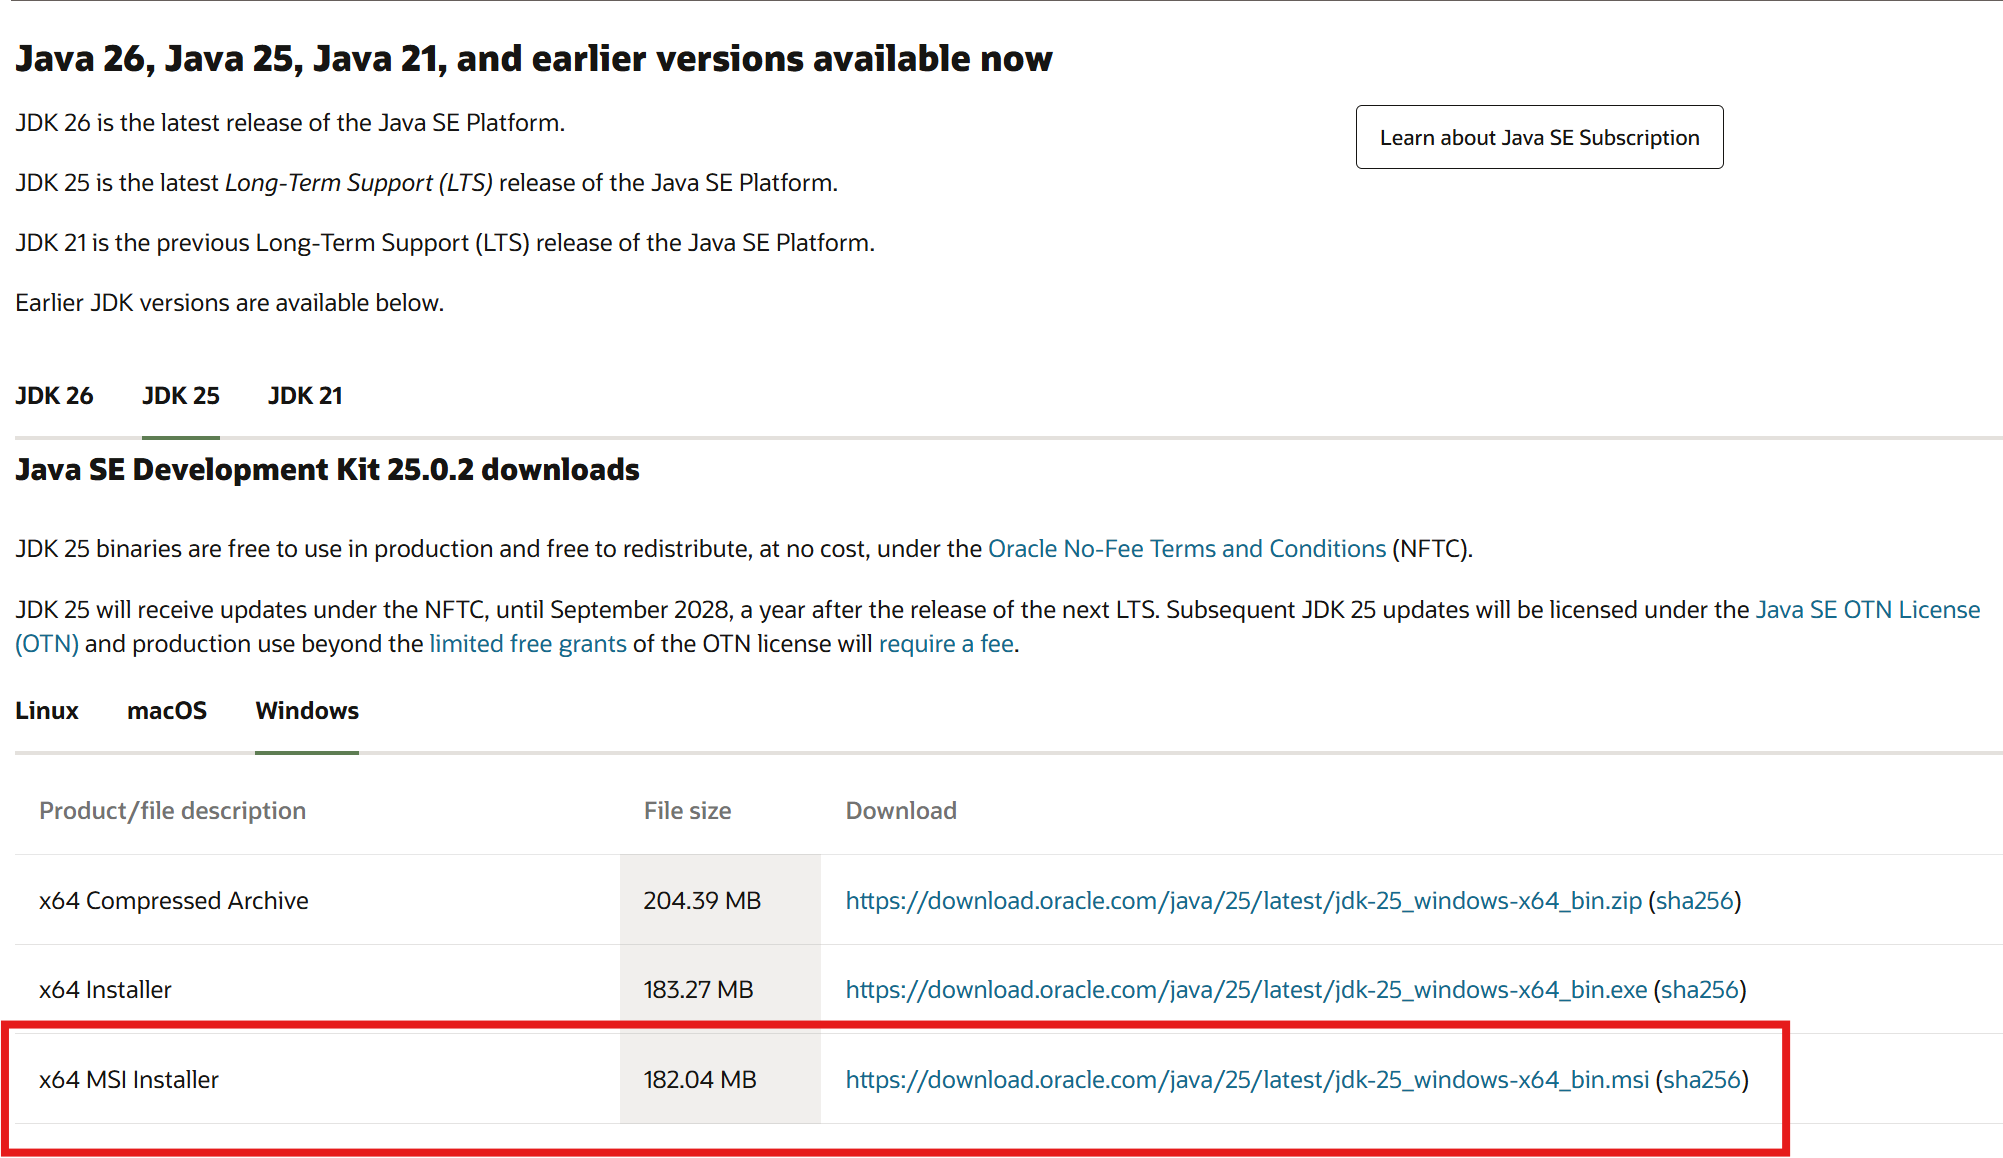
\includegraphics[width=0.75\linewidth]{image2.png}
\end{center}
\bigskip

\begin{enumerate}[resume]
\item Након тога, покренути преузету датотеку и довршити њену инсталацију.
\item По успешној инсталацији требало би да је креиран под-директоријум за одговарајућу инсталацију у оквиру директоријума „C://Program Files/Java“, на пример:
\end{enumerate}
\bigskip
\begin{center}
  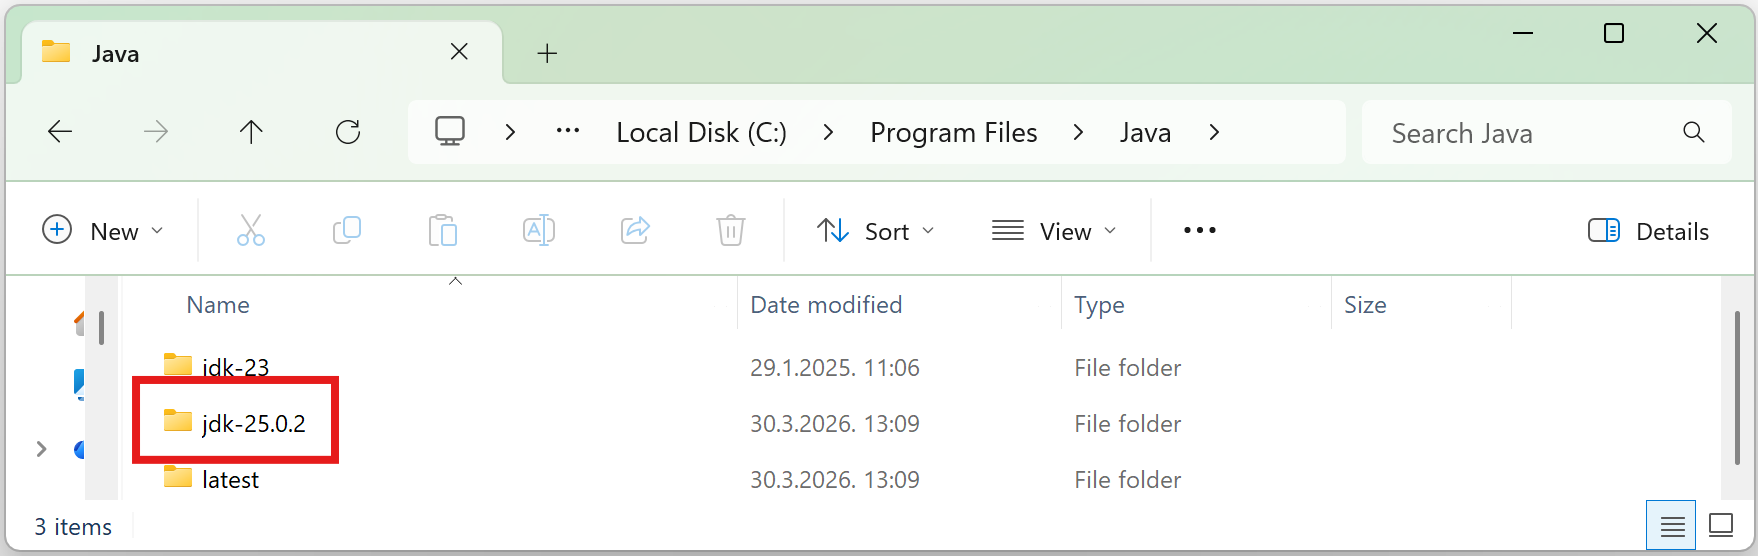
\includegraphics[width=0.75\linewidth]{image3.png}
\end{center}
\bigskip

На слици се види да је могуће имати истовремено више инсталираних JDK. Која од њих ће се користити приликом развоја програма зависи од подешавања развојног окружења.

\begin{enumerate}[resume]
\item Исправност инсталације може се проверити отварањем командне линије (Command Prompt или PowerShell) и покретањем команде:
\end{enumerate}
\begin{center}\texttt{java -version}\end{center}

Уколико је инсталација успешна, требало би да се прикаже верзија инсталиране Јаве.

\bigskip
\begin{center}
  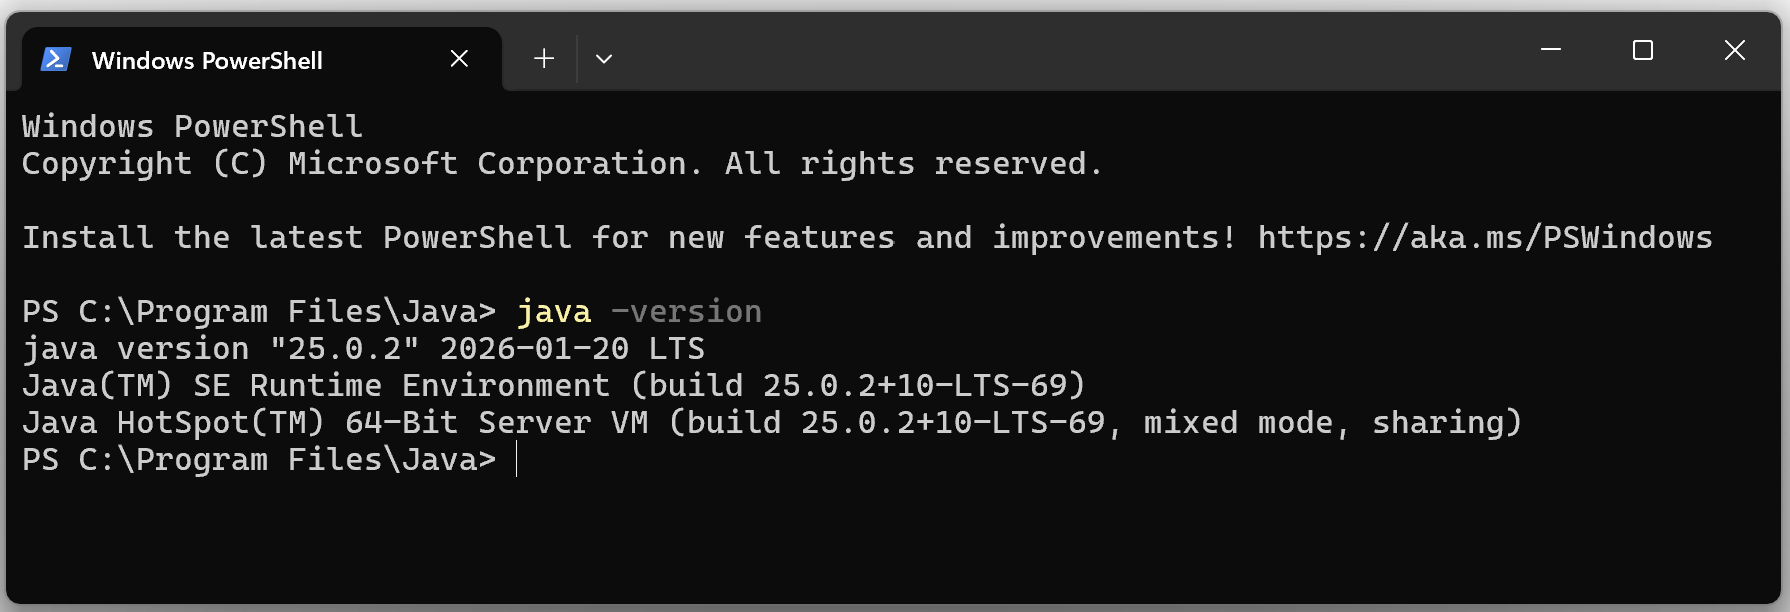
\includegraphics[width=0.75\linewidth]{image4.png}
\section{Инсталација развојног окружења IntelliJ}

\end{center}
\bigskip

Напомена: Од верзије 2025.3, IntelliJ IDEA више нема одвојено Community издање. Постоји само једно издање IntelliJ IDEA, при чему су све функционалности које је раније имало Community издање и даље бесплатне, како за комерцијалну, тако и за некомерцијалну употребу. Додатно, неке напредне функционалности (Spring, Jakarta EE, подршка за базе података, SQL) су такође постале бесплатне у основном облику.

\begin{enumerate}
\item Посетити сајт компаније JetBrains на следећој веб локацији: https://www.jetbrains.com/idea/download/
\item Преузети IntelliJ IDEA. За потребе овог курса, довољно је користити бесплатне функционалности које су укључене у основну верзију.
\end{enumerate}
\bigskip
\begin{center}
  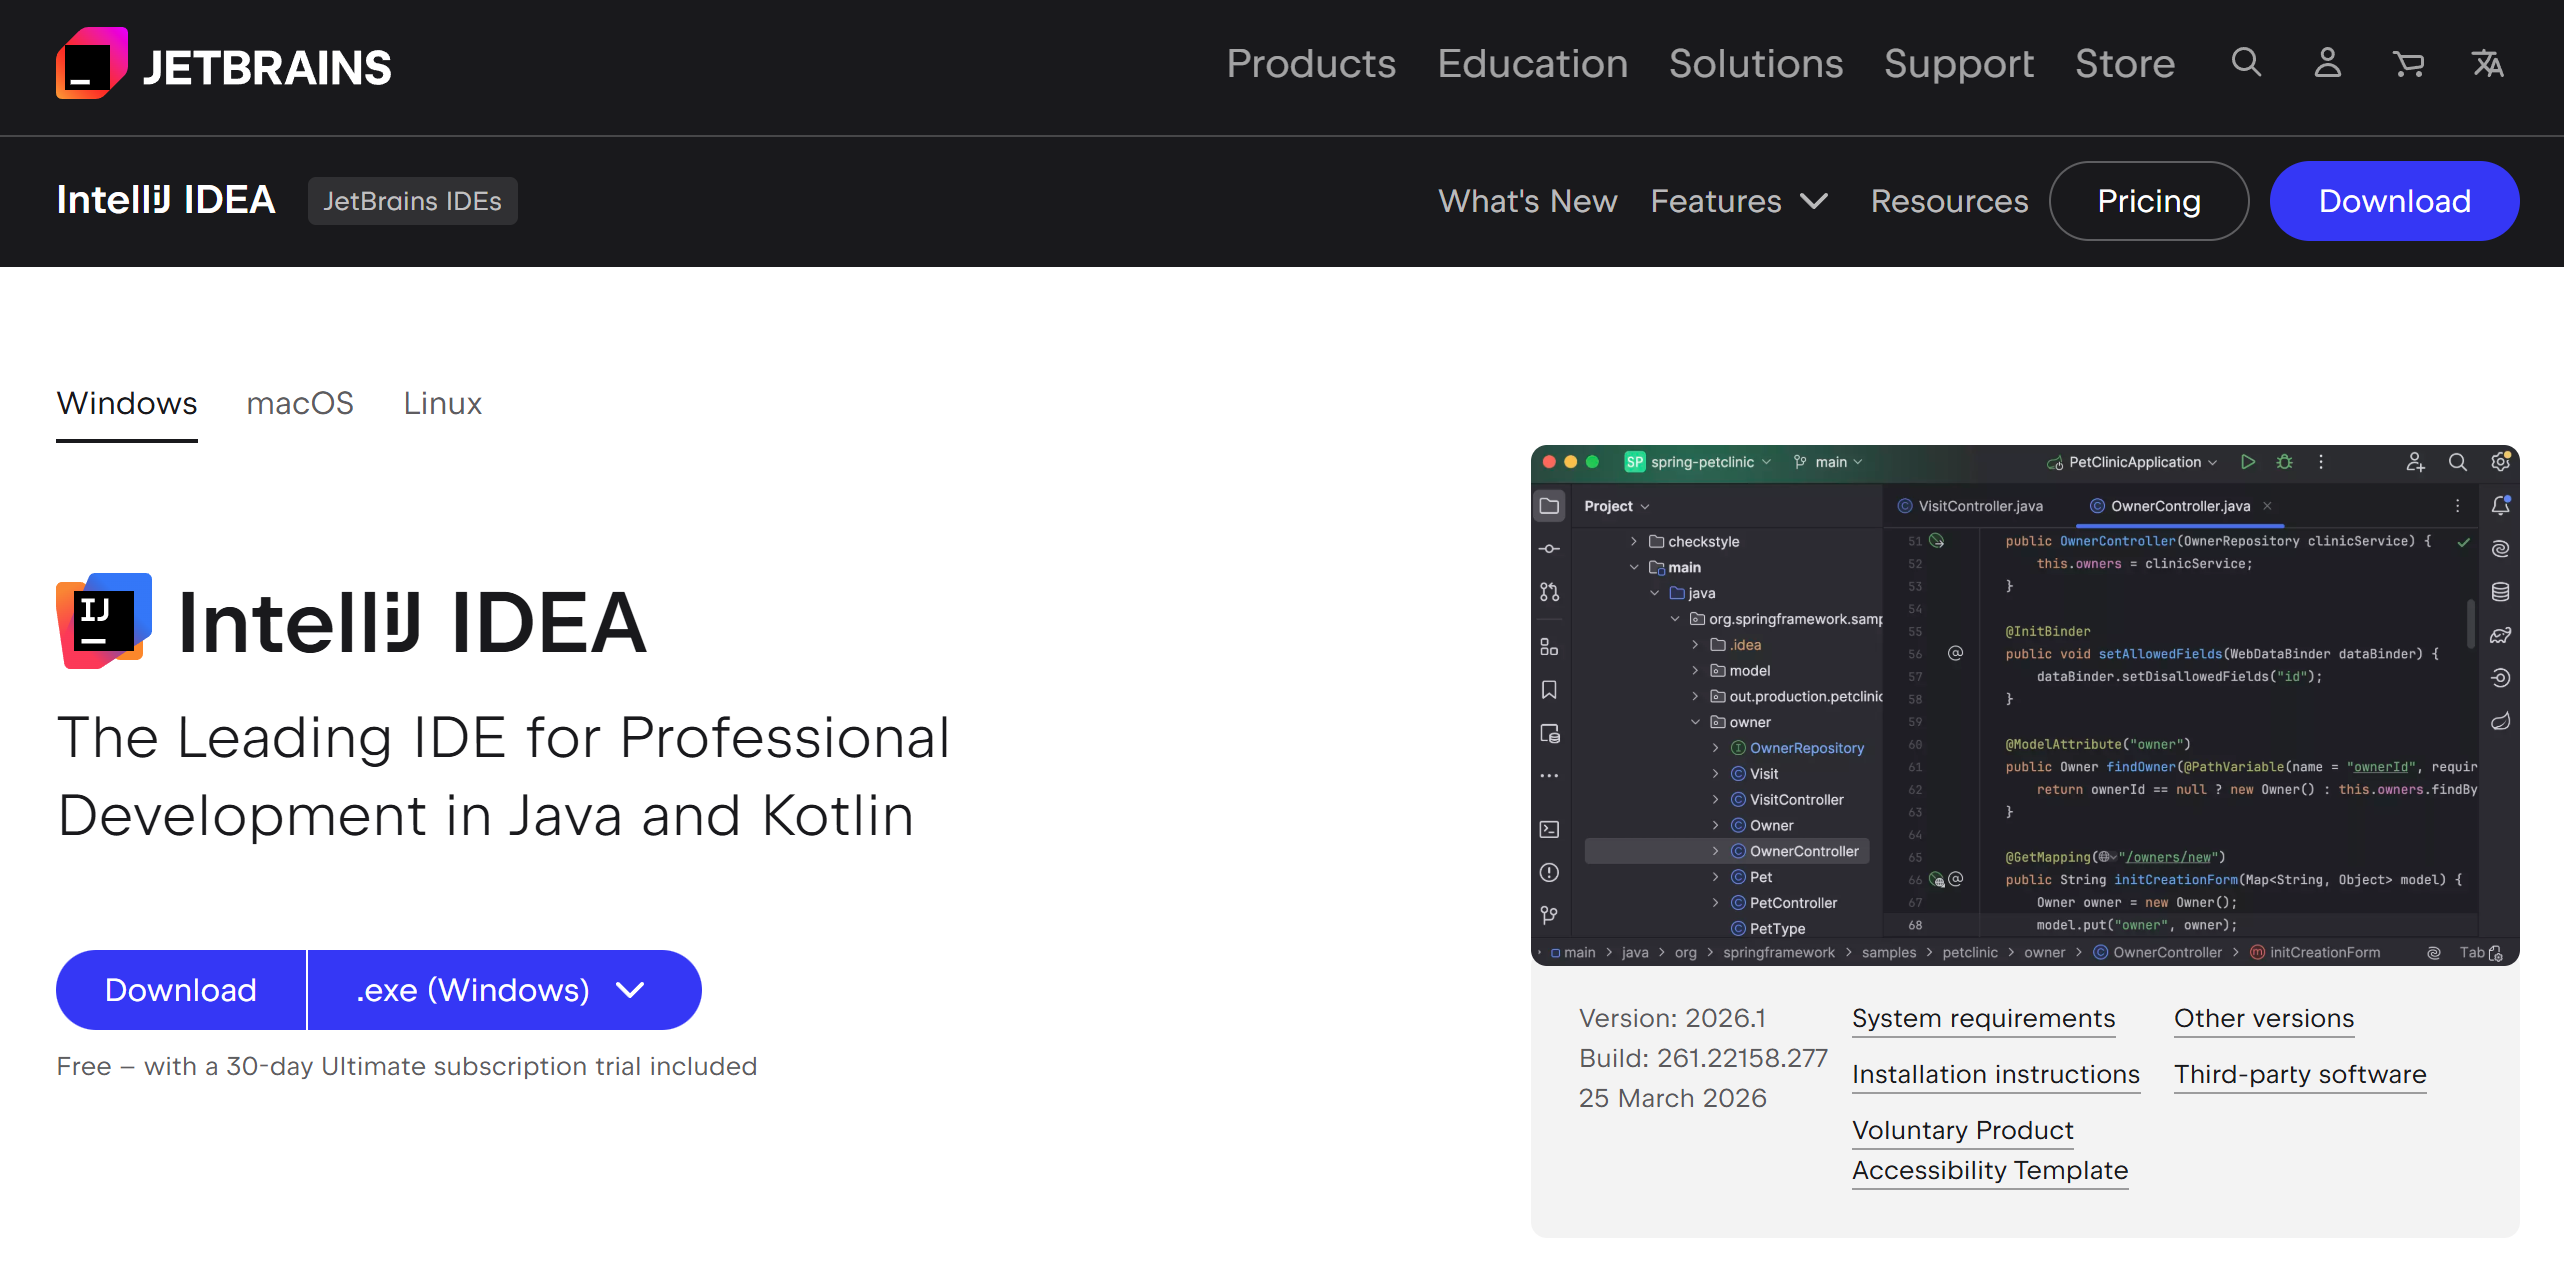
\includegraphics[width=0.75\linewidth]{image5.png}
\end{center}
\bigskip

\begin{enumerate}[resume]
\item Након преузимања покренути инсталациону датотеку и проћи кроз процес инсталације (не би требало да буде нејасних питања).
\item По завршетку инсталације могуће је одмах покренути развојно окружење, а могуће је и накнадно путем иконице на радној површини и слично.
\item Приликом покретања појавиће се питање о прихватању услова коришћења (User Agreement) које треба потврдити.
\item Почетни екран након покретања изгледа овако:
\end{enumerate}
\bigskip
\begin{center}
  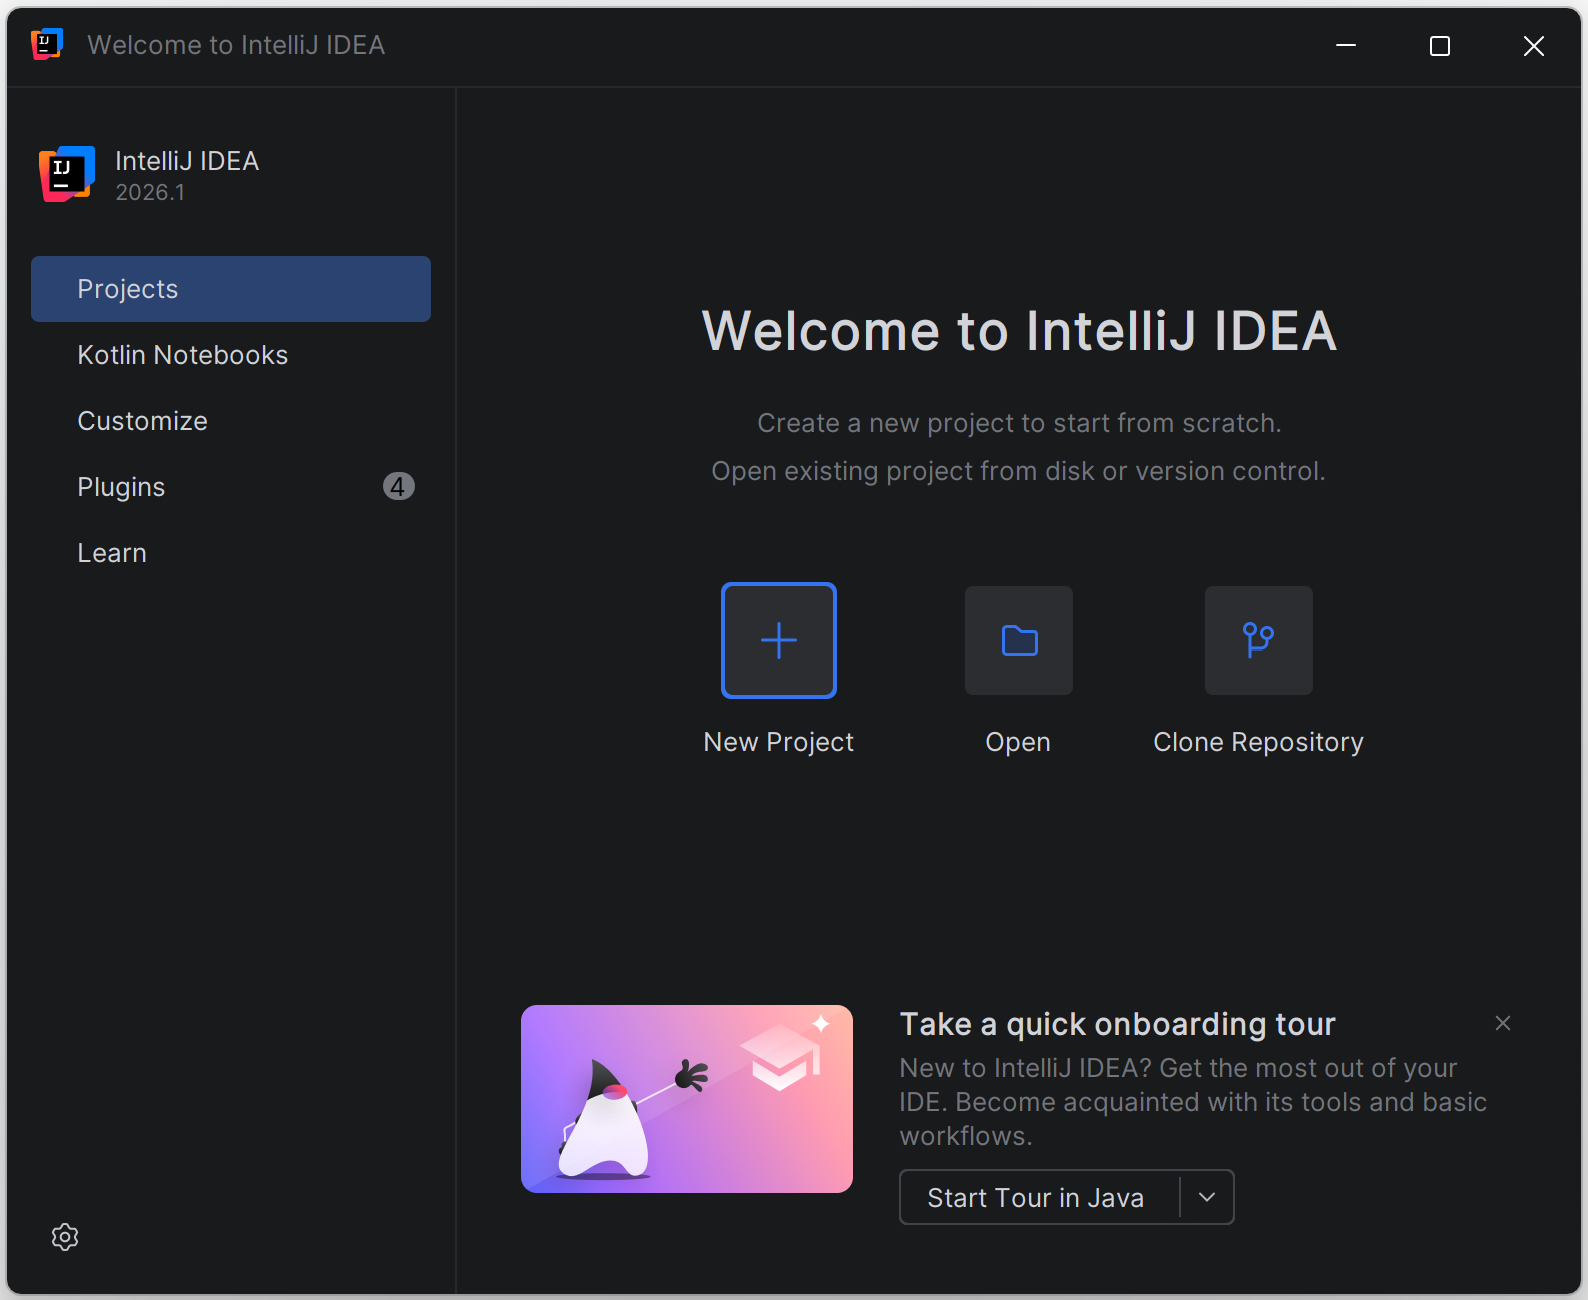
\includegraphics[width=0.75\linewidth]{image6.png}
\end{center}
\bigskip

\begin{enumerate}[resume]
\item Кликнути на опцију „New Project“. Након тога ће се појавити следећи дијалог:
\end{enumerate}
\bigskip
\begin{center}
  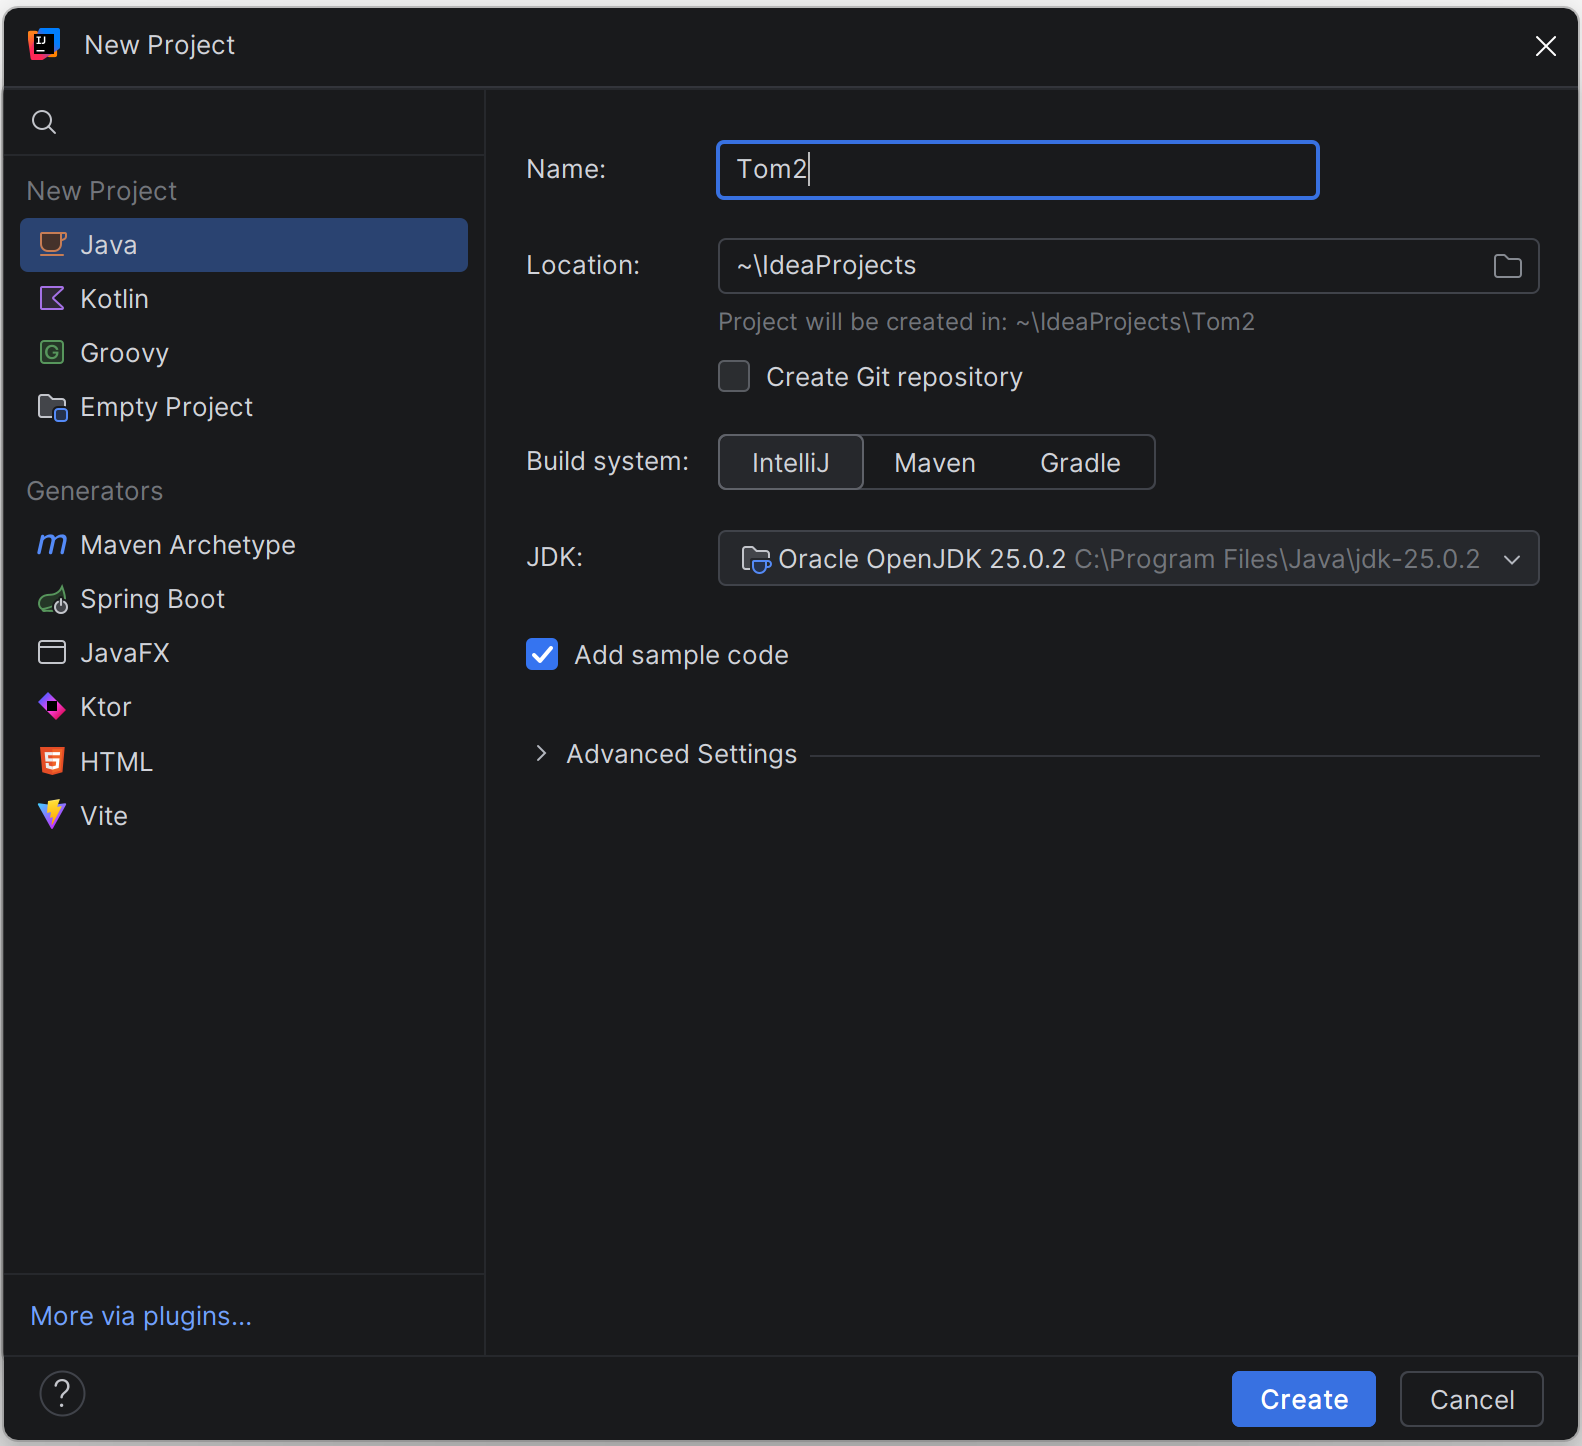
\includegraphics[width=0.75\linewidth]{image7.png}
\end{center}
\bigskip

\begin{enumerate}[resume]
\item Унети назив пројекта и проверити да ли је JDK адекватно препознат од IntelliJ окружења. Потом кликнути на дугме „Create“.
\item Тиме је завршена инсталација развојног окружења и покренут је пројекат, што би требало да изгледа, оквирно, овако:
\end{enumerate}

\bigskip
\begin{center}
  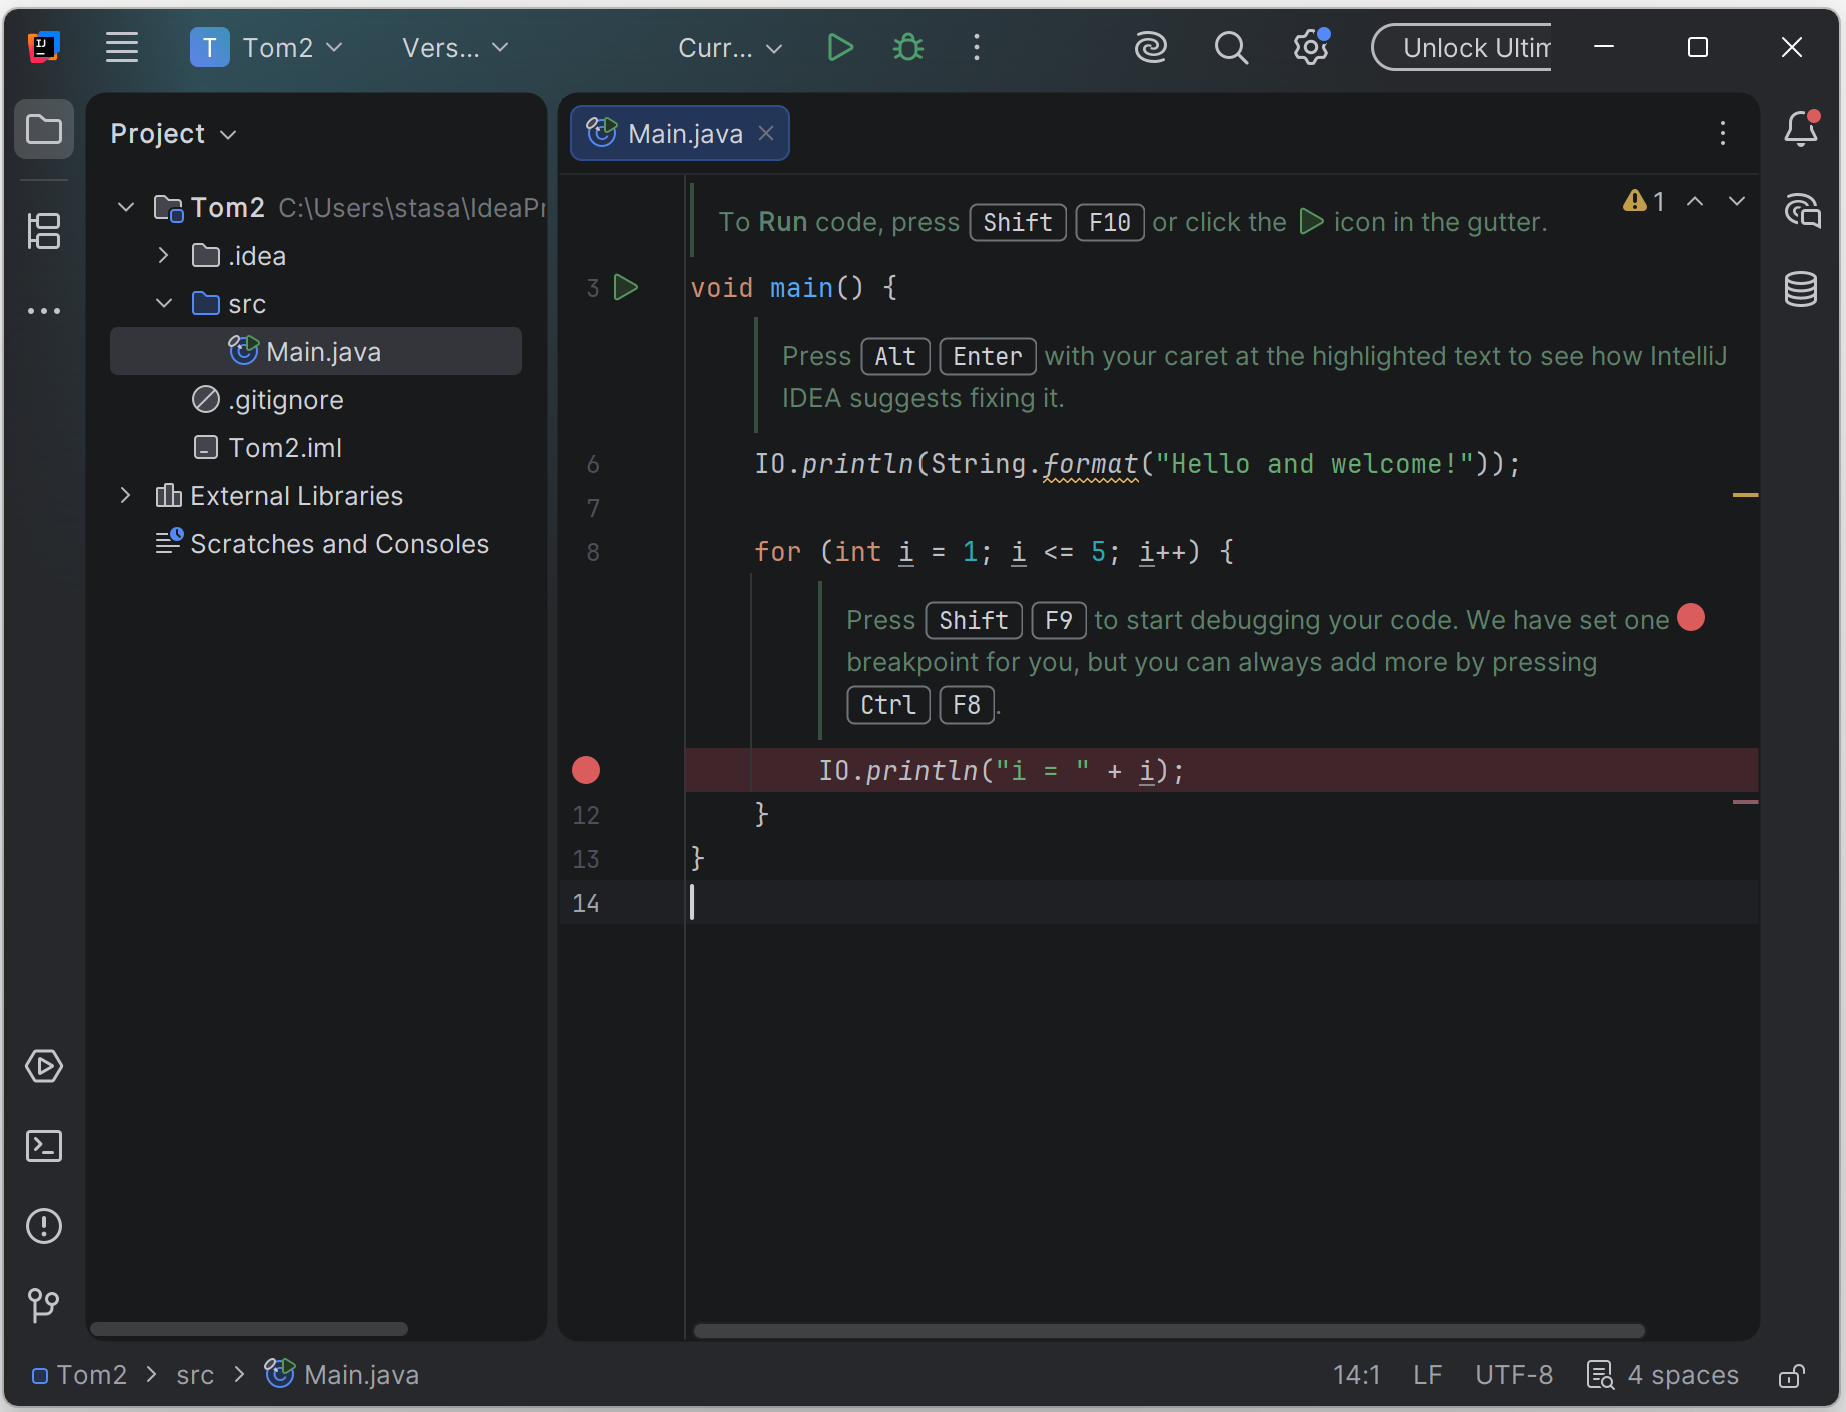
\includegraphics[width=0.75\linewidth]{image8.png}
\section{Инсталација развојног окружења Eclipse}

\end{center}
\bigskip

\begin{enumerate}
\item Посетити сајт Eclipse организације за преузимање програма, конкретно адресу: https://www.eclipse.org/downloads/
\item Преузети актуелну верзију Eclipse окружења кликом на дугме „Download x86\_64“.
\end{enumerate}
\bigskip
\begin{center}
  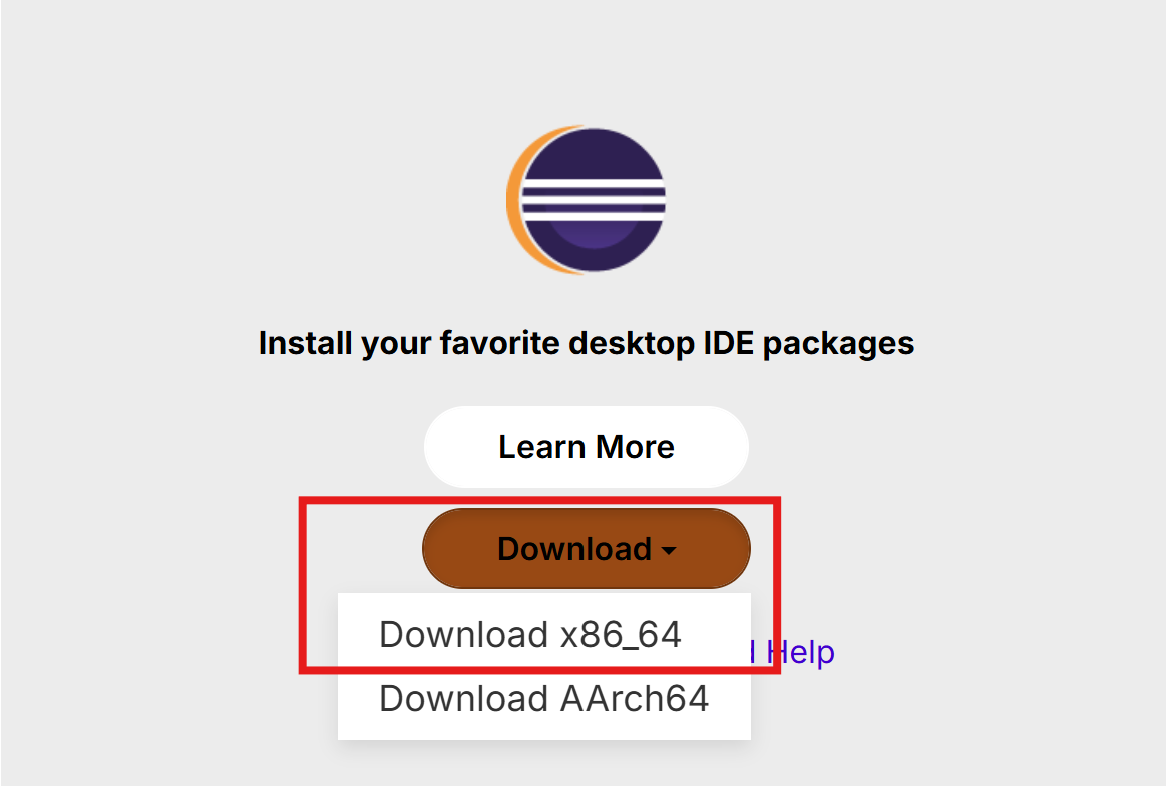
\includegraphics[width=0.75\linewidth]{image9.png}
\end{center}
\bigskip


\begin{enumerate}[resume]
\item Након тога, покренути преузету датотеку и започети њену инсталацију.
\item У оквиру првог инсталационог прозора одабрати опцију „Eclipse IDE for Java Developers“:
\end{enumerate}
\bigskip
\begin{center}
  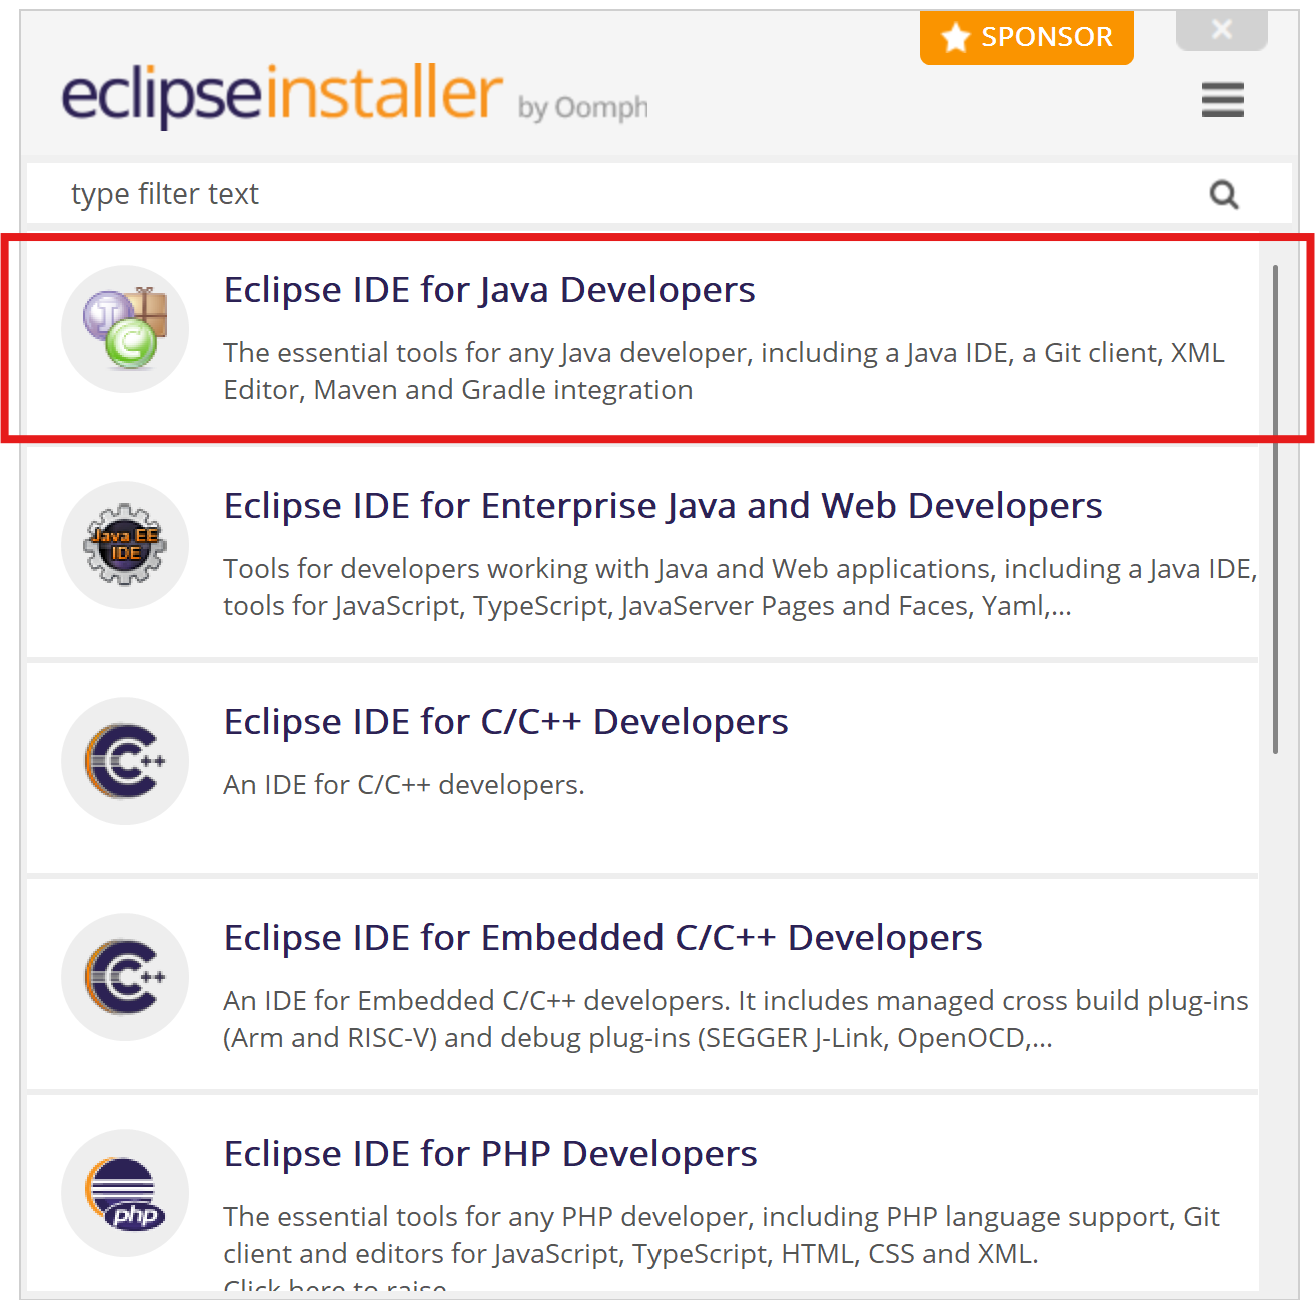
\includegraphics[width=0.75\linewidth]{image10.png}
\end{center}
\bigskip

\begin{enumerate}[resume]
\item Следећи инсталациони прозор ће укључивати неколико питања. Најважније је питање где се налази претходно инсталирана Јава.
\end{enumerate}
\bigskip
\begin{center}
  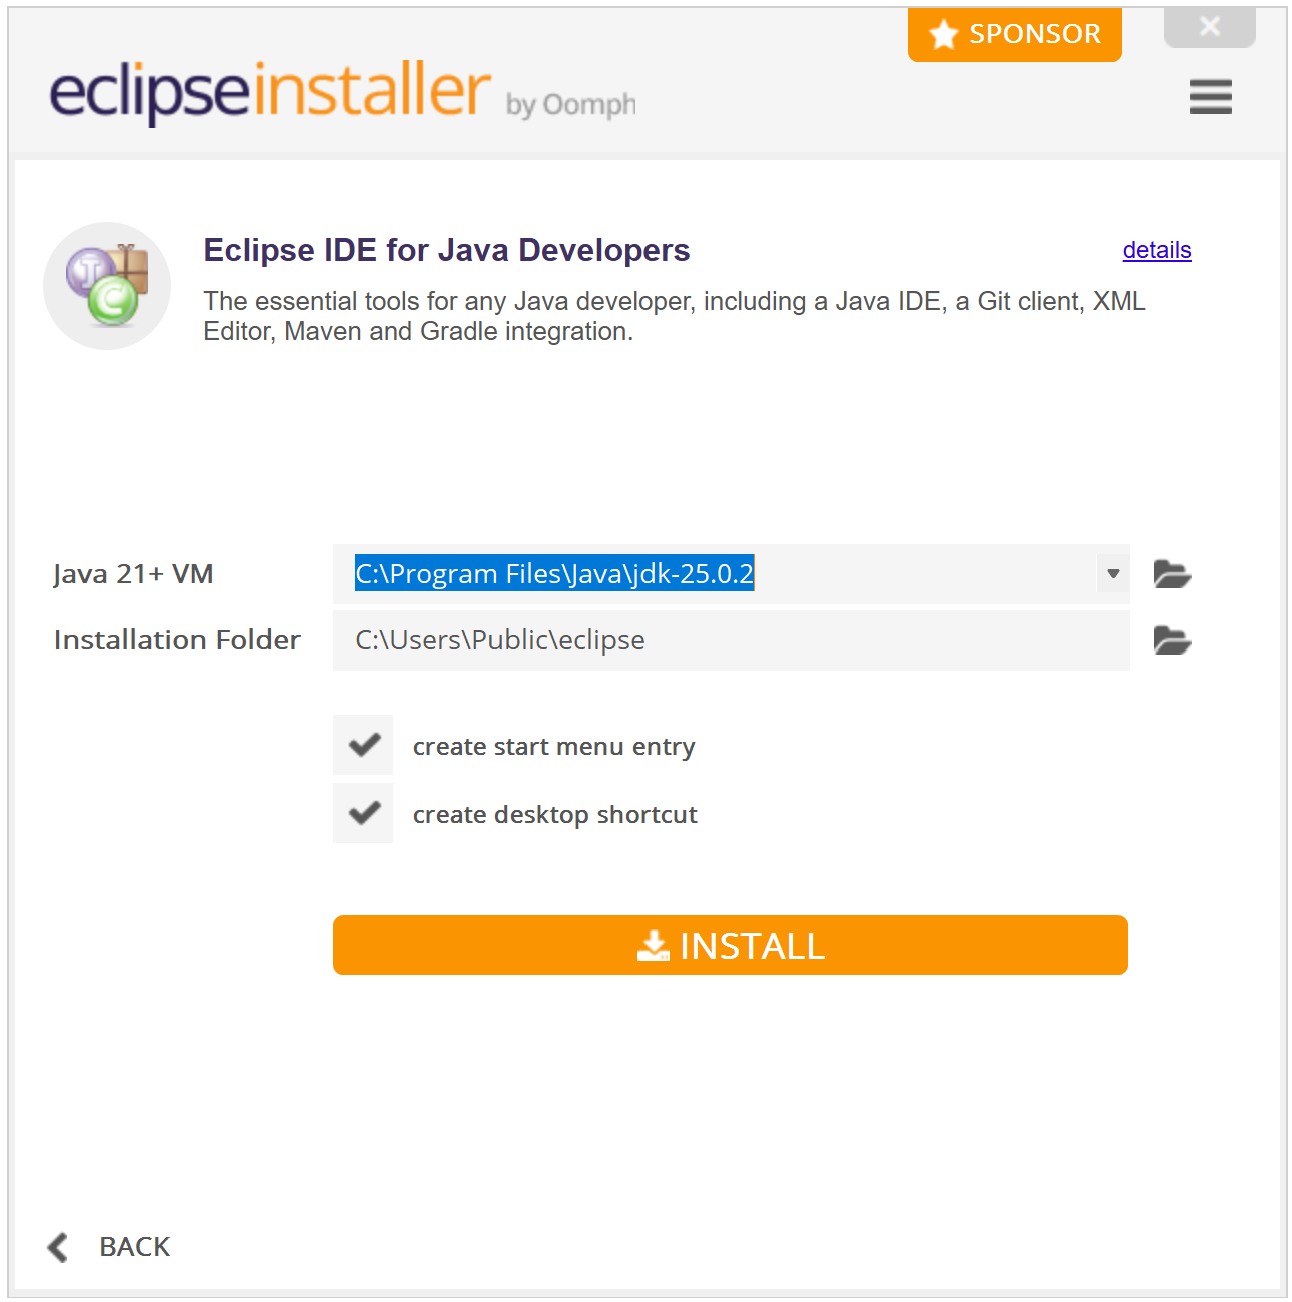
\includegraphics[width=0.75\linewidth]{image11.png}
\end{center}
\bigskip

\begin{enumerate}[resume]
\item По успешној инсталацији могуће је покренути Eclipse развојно окружење кликом на дугме „LAUNCH“ или алтернативно кликом на иконицу на радној површини.
\item Приликом покретања Eclipse, биће постављено питање где корисник жели да позиционира директоријум са кодовима (енг. \textit{workspace}). Није погрешно прихватити предложену локацију.
\end{enumerate}
\bigskip
\begin{center}
  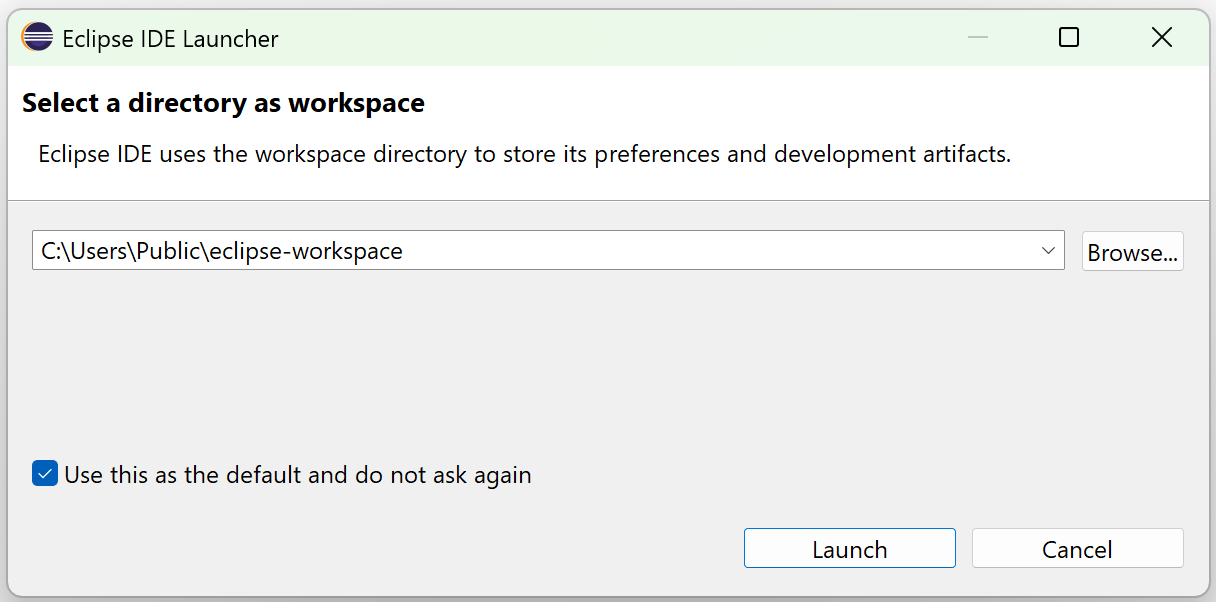
\includegraphics[width=0.75\linewidth]{image12.png}
\end{center}
\bigskip

\begin{enumerate}[resume]
\item Искључити прозор добродошлице (енг. \textit{welcome}).
\item Сада опцијом „File→New→Java Project“ и задавањем имена пројекта креирати први пројекат.
\item Следећи прозор може поставити питање у вези употребе система модула, уколико се не планира њихово коришћење, може се одабрати опција „Don’t Create“.
\item Тиме је завршена инсталација развојног окружења и покренут је пројекат, што би требало да изгледа, оквирно, овако:
\end{enumerate}
\bigskip
\begin{center}
  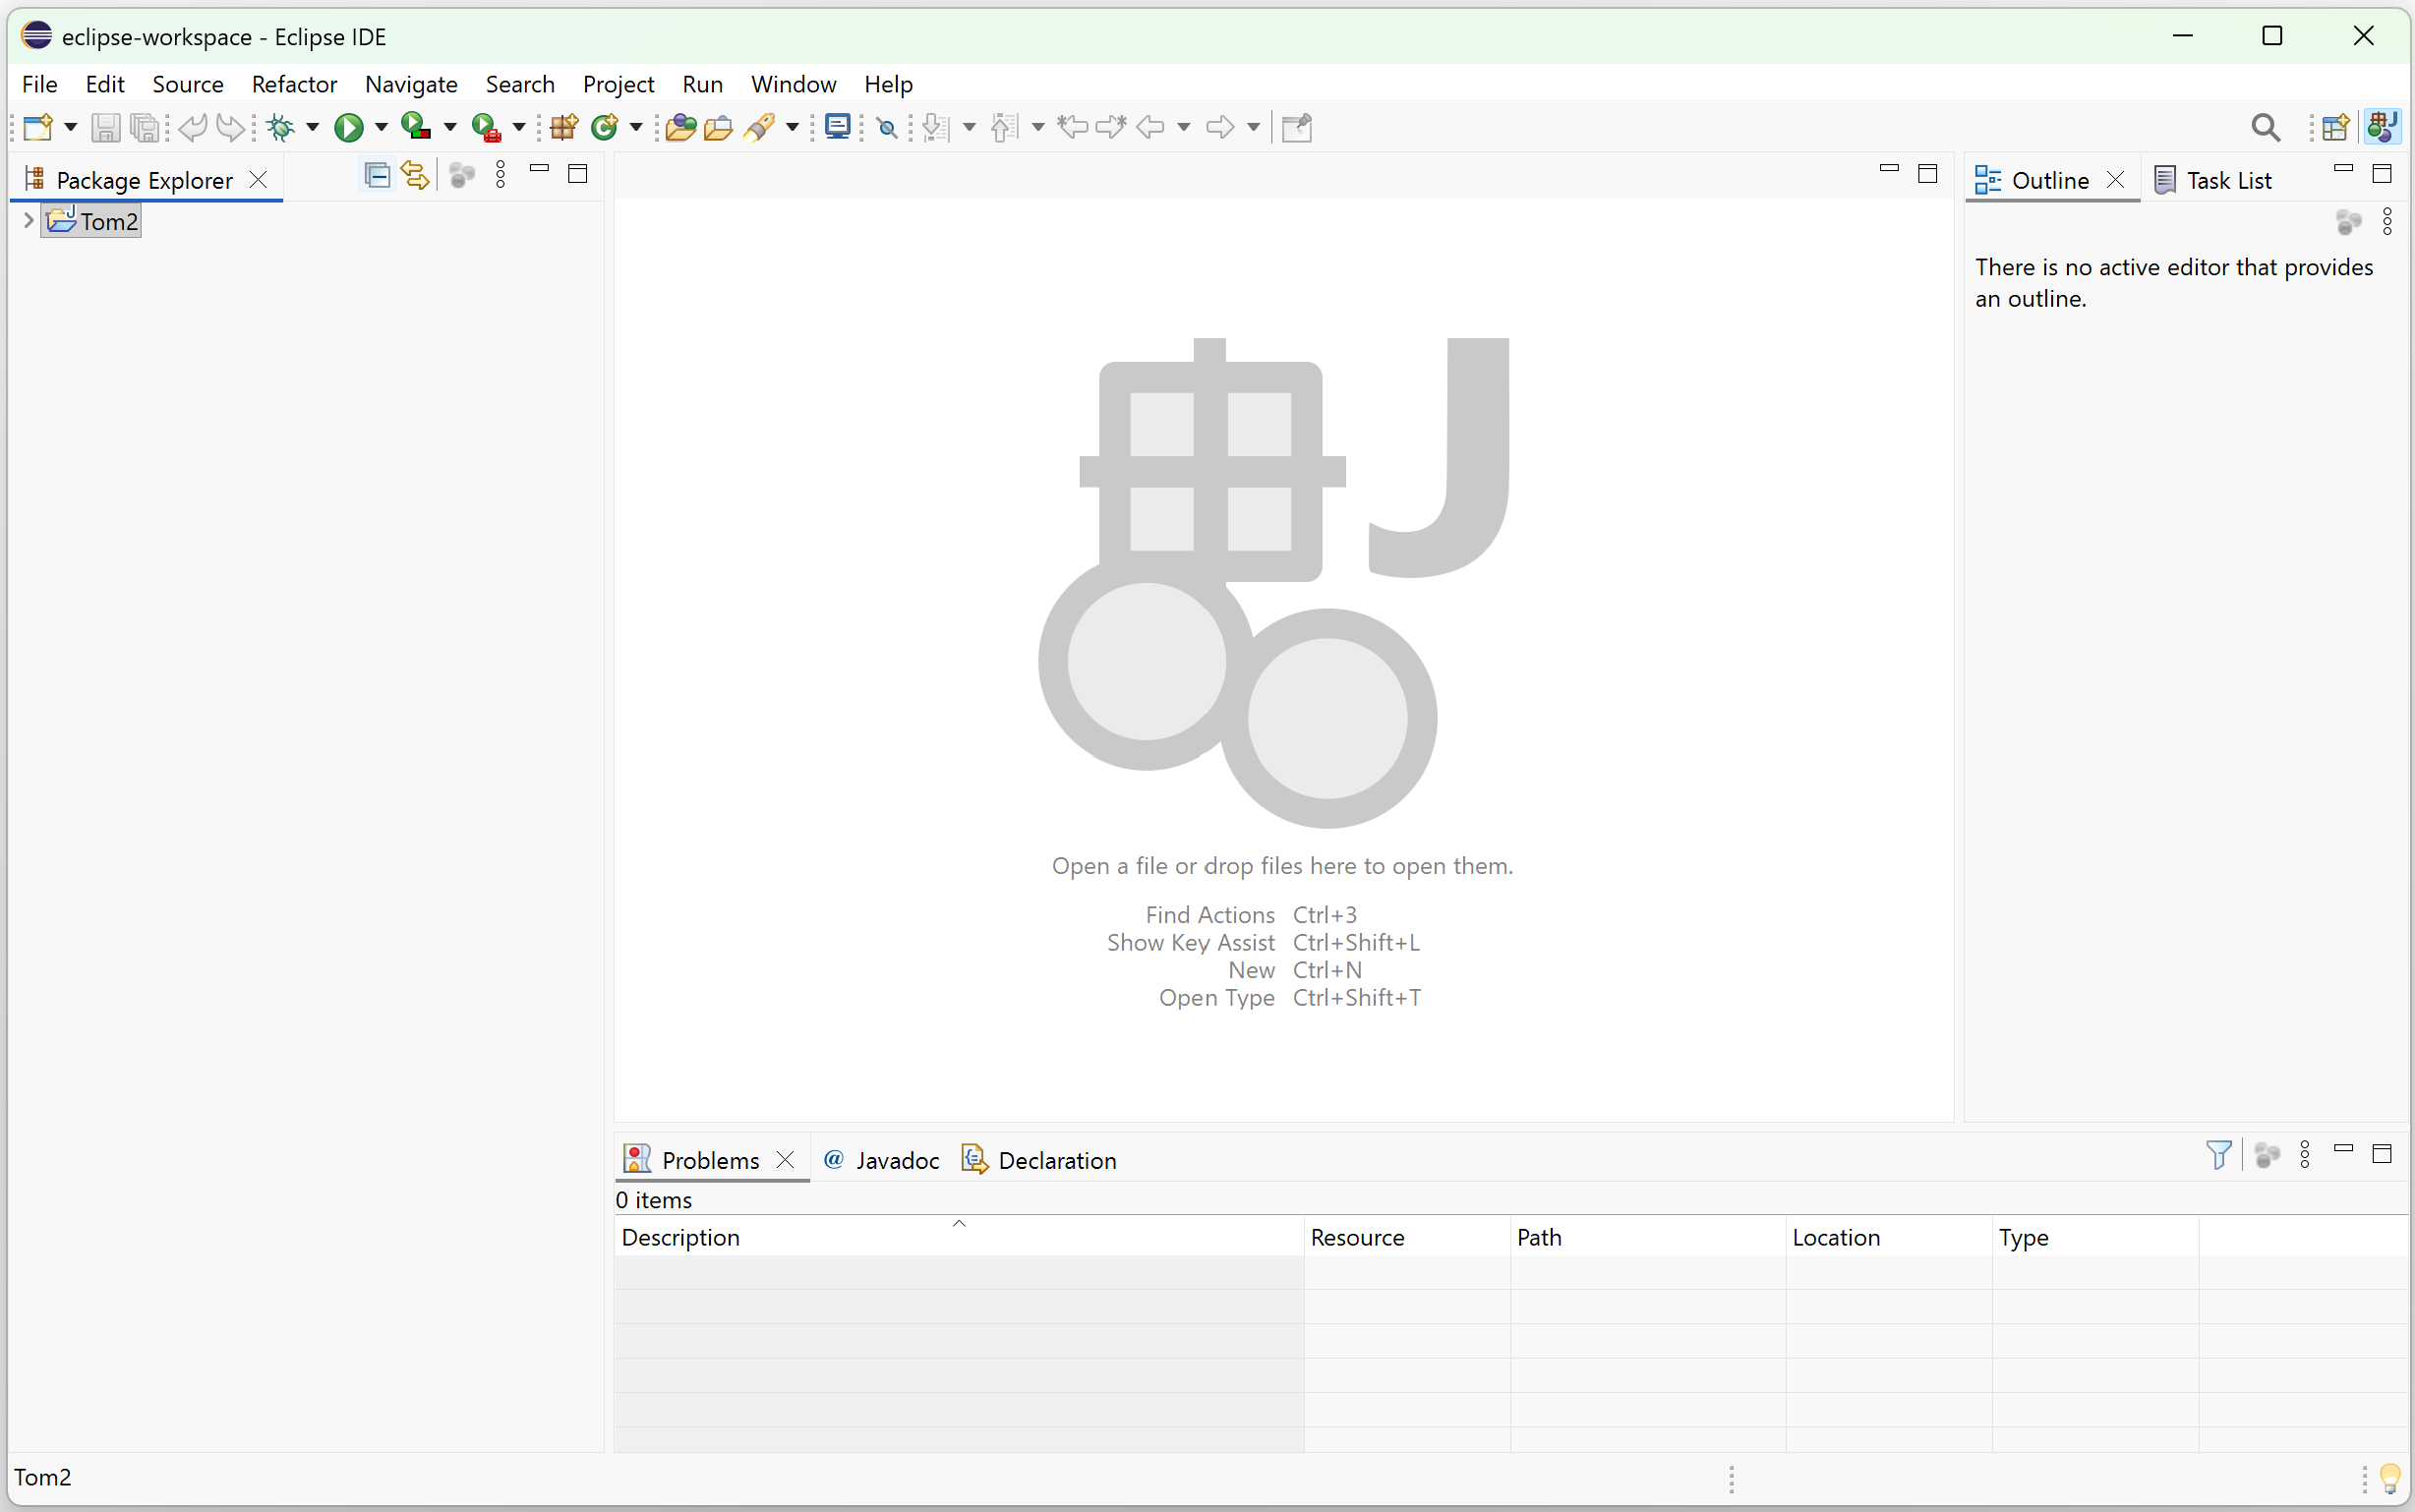
\includegraphics[width=0.75\linewidth]{image13.png}
\end{center}
\bigskip



\setlength{\parindent}{15pt}
\setlength{\parskip}{0pt}
\cleardoublepage
\thispagestyle{plain}
\phantomsection
\addcontentsline{toc}{chapter}{Додатак Б -- Упутство за употребу GitHub репозиторијума и подешавање ћирилице}
\markboth{Додатак Б}{Додатак Б}
\vspace*{50pt}
{\raggedright\huge\bfseries Додатак Б\par}
\vskip 20pt
{\raggedright\Huge\bfseries Упутство за употребу GitHub репозиторијума и подешавање ћирилице\par}
\vskip 12pt
{\color{black!50}\hrule height 0.4pt}
\vskip 30pt
\pagestyle{plain}
\setcounter{section}{0}
\renewcommand{\thesection}{Б.\arabic{section}}
\renewcommand{\thesubsection}{Б.\arabic{section}.\arabic{subsection}}

Сви примери коришћени у књизи налазе се на GitHub репозиторијуму:

https://github.com/matf-oop-java/tom-2.

Следи упутство за преузимање (клонирање) овог репозиторијума и његову интеграцију са претходно наведеним развојним окружењима IntelliJ и Eclipse.

\section{Структура репозиторијума}

Репозиторијум садржи следеће датотеке и директоријуме:

\begin{enumerate}
\item src/ – изворни код свих примера из књиге, организован у пакете по главама.
\item resources/ – ресурсне датотеке (XML, properties, persistence.xml) потребне за извршавање примера.
\item build.gradle – Gradle конфигурација која аутоматски преузима све потребне библиотеке са интернета.
\item gradlew/gradlew.bat – скрипте за покретање Gradle-а без претходне инсталације (Gradle wrapper).
\end{enumerate}
\section{Преузимање репозиторијума}

Кодови и пратећи подаци се могу преузети на два начина: у виду .zip архиве или клонирањем помоћу Git алата.

\textbf{Начин 1: Преузимање .zip архиве}

\begin{enumerate}
\item Посетити веб сајт: https://github.com/matf-oop-java/tom-2
\item Кликнути на зелено дугме „Code“ и одабрати опцију „Download ZIP“.
\item Након преузимања, архиву распаковати на погодној локацији.
\end{enumerate}
\textbf{Начин 2: Клонирање помоћу Git-а}

Уколико је Git инсталиран, репозиторијум се може клонирати из командне линије:

\begin{center}\texttt{git clone https://github.com/matf-oop-java/tom-2.git}\end{center}

Алтернативно, може се користити графички клијент GitHub Desktop, који омогућава клонирање кликом на дугме „Open with GitHub Desktop“ на веб страници репозиторијума.

\section{Учитавање материјала у IntelliJ пројекат}

\begin{enumerate}
\item Покренути IntelliJ IDEA и изабрати „File → Open“.
\item Пронаћи директоријум преузетог репозиторијума и кликнути „Open“.
\item IntelliJ ће препознати датотеку build.gradle и понудити да увезе пројекат као Gradle пројекат. Кликнути „OK“ односно „Trust Project“.
\item Сачекати да IntelliJ заврши увоз и индексирање (трака напретка при дну екрана). Током овог процеса Gradle аутоматски преузима све потребне библиотеке са интернета.
\item Проверити JDK: отворити „File → Project Structure“ и у одељку Project проверити да је SDK подешен на JDK 25 и Language level на 25.
\item Подесити кодирање: отворити „File → Settings → Editor → File Encodings“ и поставити Global Encoding, Project Encoding и Default encoding for properties files на UTF-8.
\item Подесити делегирање покретања: отворити „File → Settings → Build, Execution, Deployment → Build Tools → Gradle" и променити „Build and run using" на Gradle и „Run tests using" на Gradle. Ово је обавезно да би сви примери (укључујући JavaFX) исправно радили.
\item Кликнути Apply, затим OK. Пројекат је спреман за рад.
\end{enumerate}
Напомена: Библиотеке се аутоматски преузимају преко Gradle-а и не морају се ручно додавати. За покретање JavaFX примера (глава 5) такође није потребна додатна конфигурација. Gradle JavaFX додатак аутоматски подешава потребне модуле.

\section{Учитавање материјала у Eclipse пројекат}

\begin{enumerate}
\item Покренути Eclipse развојно окружење.
\item Изабрати опцију „File → Import... → Gradle → Existing Gradle Project“.
\item Кликнути на дугме „Browse...“ и пронаћи директоријум преузетог репозиторијума. Кликнути „Finish“.
\item Eclipse ће аутоматски покренути Gradle и преузети све потребне библиотеке са интернета. За ово је потребна интернет конекција.
\item Подесити JDK: кликнути десним тастером на пројекат → Properties → Java Build Path → картица Libraries → подесити JRE System Library на JDK 25.
\item Подесити кодирање: отићи на „Window → Preferences → General → Workspace“ и поставити „Text file encoding“ на UTF-8. Ово је неопходно за исправан приказ ћириличног писма.
\item Након тога би требало да су сви примери функционални, да нема грешака и да се ћирилично писмо уредно приказује у Јава текстуалном едитору.
\end{enumerate}


\chapter*{Литература}
\addcontentsline{toc}{chapter}{Литература}
\markboth{Литература}{Литература}
\pagestyle{empty}
\thispagestyle{empty}
\setlength{\parindent}{0pt}
\setlength{\parskip}{4pt}


Arnold K, Gosling J, Holmes D: Programski jezik Java, CET, Beograd, 2001.

Arnold K, Gosling J: The Java Programming Language, Addison-Wesley, 1996.

Bauer C, King G, Gregory G: Java Persistence with Hibernate, 2nd Ed, Manning, 2015.

Bloch J: Effective Java, 3rd Ed, Addison-Wesley, 2018.

Čabarkapa M: Računarstvo i informatika – udžbenik sa zbirkom zadataka za 4. razred gimnazije prirodno-matematičkog i opšteg smera, Krug, Beograd, 2008.

Eckel B: Thinking in Java, 4th Ed, Prentice Hall, 2006.

Gamma E, Helm R, Johnson R, Vlissides J: Design Patterns: Elements of Reusable Object-Oriented Software, Addison-Wesley, 1994.

Goetz B, Peierls T, Bloch J, Bowbeer J, Holmes D, Lea D: Java Concurrency in Practice, Addison-Wesley, 2006.

Horstmann C: Core Java, Volume I – Fundamentals, 12th Ed, Prentice Hall, 2022.

Horstmann C: Core Java, Volume II – Advanced Features, 12th Ed, Prentice Hall, 2022.

Horton I: Java 2 – JDK 1.5, CET, Beograd, 2006.

Lemay L, Cadenhead R: Java 1.2, Kompjuter biblioteka, Čačak, 2001.

Mak R: Java for the Real World, Manning, 2025.

Schildt H: Java – The Complete Reference, 13th Ed, McGraw-Hill, 2024.

Tošić D: Računarstvo i informatika za III razred gimnazije, Zavod za udžbenike, Beograd, 2011.

Tudose C: JUnit in Action, 3rd Ed, Manning, 2020.

Urma R, Fusco M, Mycroft A: Modern Java in Action, 2nd Ed, Manning, 2019.

Walls C: Spring in Action, 6th Ed, Manning, 2022.


Baeldung – Java Tutorials: https://www.baeldung.com/

Jakarta EE Documentation: https://jakarta.ee/specifications/

Java SE Documentation: https://docs.oracle.com/en/java/javase/

Java Tutorials: https://docs.oracle.com/javase/tutorial/

JUnit 5 User Guide:  https://junit.org/junit5/docs/current/user-guide/

Oracle Java: https://www.oracle.com/java/


\end{document}
